\documentclass[letterpaper, 10pt, openright]{memoir}

%0ther
\renewcommand{\and}{\\\vskip 1em}
\def\headline#1{\hbox to \hsize{\hrulefill\quad\lower.3em\hbox{#1}\quad\hrulefill}}
\newcommand{\doendnotes}{%
	\markright{Notes}
	\theendnotes
	\setcounter{endnote}{0}
}
\newcommand{\doubleline}{%
	\hrule height 3\normalrulethickness
	\vskip 0.25em
	\hrule height \normalrulethickness
}

%Table of Contents
\makeatletter
\def\cftsectionpresnum #1\@cftasnum{}
\makeatother
\setlength\cftchapternumwidth{3em}
\cftpagenumbersoff{chapter}
\renewcommand{\contentsname}{\huge{Table} \Large{of} \huge{Contents}}

%Chapter style
\makechapterstyle{custom} {%
	\renewcommand{\thechapter}{\Roman{chapter}}
	\renewcommand{\chapterheadstart}{}
	\renewcommand{\printchaptername}{}
	\renewcommand{\chapternamenum}{}
	\renewcommand{\printchapternum}{\headline{\huge Chapter \thechapter}}
	\renewcommand{\afterchapternum}{}
	\renewcommand{\printchaptertitle}[1]{%
		\raggedright\huge\scshape\MakeLowercase{##1}}
	\renewcommand{\afterchaptertitle}{%
		\vskip\onelineskip \hrule\vskip\onelineskip}
}
\chapterstyle{custom}

%Section
\renewcommand{\thesection}{\Roman{section}}
\setsecheadstyle{\raggedright\scshape\large}
\setbeforesecskip{-\onelineskip}
\setaftersecskip{\onelineskip}
\setsecnumformat{}
\renewcommand{\sectionmark}[1]{\markboth{Chapter \thechapter.}{Part \thesection.}}

%subsection
\setsubsecheadstyle{\sethangfrom{\noindent ##1}\raggedright\itshape}
\setbeforesubsecskip{-\onelineskip}
\setaftersubsecskip{\onelineskip}

%EndNotes
\makepagenote
\renewcommand{\idtextinnotes}[1]{\footnotesize#1)\space}
\renewcommand{\prenoteinnotes}{\par\noindent\hangindent 2em}
\renewcommand{\prenotetext}{\begingroup\footnotesize}
\renewcommand{\postnotetext}{\endgroup}
\renewcommand{\notedivision}{%
	\headline{\huge\notesname}\vskip\onelineskip
	\markboth{Chapter \thechapter.}{\notesname}
	\thispagestyle{simple}
}
\renewcommand{\pagenotesubhead}[3]{}

\begin{document}
\frontmatter
\pretitle{\begin{center}\bfseries}
\title{%
	\small{THE}\\\vskip 1em
	\Huge{HISTORY}\\\vskip 1em
	\small{OF THE}\\\vskip 1em
	\Large{DECLINE AND FALL}\\\vskip 1em
	\small{OF THE}\\\vskip 1em
	\Huge{ROMAN EMPIRE}
}
\posttitle{\end{center}\vskip 1em}
\preauthor{\begin{center}\large\bfseries}
\author{%
	Edward Gibbon, \textit{Esq.}
	\and  With notes by the Rev. H. H. Milman
	\and Vol. 1}
\postauthor{\end{center}}
\predate{\begin{center}}
\date{\bfseries\normalsize 1782 (Written), 1845 (Revised)}
\postdate{%
	\end{center}
	\vskip 1em
	\doubleline
}

\maketitle


\tableofcontents*
\begin{flushleft}
\fontsize{35}{35}\sffamily
\textbf{Man, His Origin and Destiny}
\Large{by Joseph Fielding Smith}
\end{flushleft}

\section{FOREWORD}
\thispagestyle{empty}

Conflicting attitudes expressed concerning science and religion have confused many people.
Especially has this been true in the class room where hypotheses have been set forth
erroneously as facts and where deductions made from those theories have been regarded as
established truth.

Many of the followers of Darwin, for instance, carried his views to the extreme of
materialistic atheism, declaring not only that creation occurred without the aid of any
Intelligent Creator, but that as a matter of fact, no such Being even exists.
Both science and religion have suffered as a result. The greatest damage, however, has been
among students who have lost their faith in God through accepting these man-made theories
as facts.

But time changes things. Whereas for years atheistic deductions were made from scientific
research, now true scientists, armed with what they term "the new knowledge," are revising
their "hasty first conclusions" as Sir James Jeans expressed it, and have discovered "evidence
of a designing or controlling power that has something in common with our individual
minds."

The present day attitude of top scientists was expressed recently by Dr. Joseph W. Barker,
president and chairman of the Research Corporation of America, and formerly dean of the
engineering school at Columbia University, in an address at Ripon University. He explained
there that scientists of the nineteenth century were misled by certain of their observations,
and as a result came to conclusions which were definitely atheistic.

"But now," said Dr. Barker, "even the most pragmatic materialist, in the face of present day
scientific knowledge, is led to the inevitable conclusion that the heavens declare the glory of
God and the firmament showeth his handiwork."

Dr. Barker's concluding remarks to the students were: "As the children of Israel foreswore
the worship of the golden calf and returned to the faith of Jehovah, so have we foresworn the
crass mechanistic materialism and returned to that faith in God of which the Psalmist of old
sang. The Earth is the Lord's and all that therein is."

Knowing the great need to provide Latter-day Saint students of science with material which
would help them to preserve their faith and coordinate in their minds the pure truth of both
science and revelation, some of us have hoped for a book which could make the facts readily
available to them.

Many have recognized in President Joseph Fielding Smith of the Council of the Twelve the
profound student of scripture which he is, but not so many were acquainted with the fact that
he also is a deep student of science, widely read in various phases of the subject.

Recognizing his possession of this superb knowledge of both science and religion, some of
us urged him to write a book on the creation of the world and the origin of man, setting forth
both the up-to-date views of science, and the facts provided through revelation.

The present volume is the result. It is a most remarkable presentation of material from both
sources under discussion. It will fill a great need in the Church, and will be particularly
invaluable to students who have become confused by the misapplication of information
derived from scientific experimentation.

It will be an outstanding addition to a list of this author's books which already have stabilized
the faith of countless thousands the world around.

\vspace{\onelineskip}
-MARK E. PETERSEN.

\newpage
\section{AN INTRODUCTION}

\begin{flushleft}
BY DR. MELVIN A. COOK
\end{flushleft}

Theory plays an important role in all arts and sciences (1) by providing a means for the
unification and classification of available knowledge, and (2) by suggesting and prescribing
the design of experimental studies that will broaden the scope of knowledge. Failure to
accomplish either of these objectives necessitates modifications in the theory or substitution
of an alternate one. For this reason the basic concepts are continually undergoing change in a
healthy and forward-moving science. We are living in a world of great endeavor and
achievement in which the scientific or objective application of theory, whether true or simply
the best that can be devised to represent as faithfully as possible all known facts, has an
important place. Unfortunately, owing to the strong desire of scientists to display their
brilliance and ingenuity, there is a tendency for theory to become the objective instead of a
means to the end. Theory then not only loses its real value, but actually becomes a stumbling
block to progress. Its inventor and disciples become so engrossed in the theory that they lose
sight of its fundamental purpose, the quest for truth. This condition was shockingly
illustrated in my presence at a meeting of scientists when one of great renown met a factual
objection with the statement, "I am more concerned with the elegance of the theory than the
truth of it."

One need not look far into science to discover it consists too generally of a maze of facts and
theory so closely interwoven that even the most learned and honorable scientist (to say
nothing of the intellectually dishonest one or the novice) may have difficulty in
distinguishing readily between truth and theory. While this weakness of science is serious
enough in fields which are not closely related to the primary purposes of mortality, in the
fields more closely related, the difficulties of discerning fact and theory may well prove
disastrous. This is particularly true as regards the development of spirituality in those who
place science foremost.

The principles of the Gospel of Jesus Christ provide faithful members of the Church with
wonderful and inspiring principles of truth directly applicable in distinguishing between
fundamental truth and error in all fields of arts and science. This application requires a clear
recognition of the pre-eminence of the gospel and its "eternal scientists" of which the author
of this book stands high among the great ones in mortality. The paramount key to this
important application of "eternal science" is that every principle of the baser sciences must
square with the revealed truths.

Few fields of science come into such direct conflict with the revealed scriptures as the
palaeo-sciences—historical geology, palaeoethnology, paleontology, and palaeogeography.
The factual or experimental components of these sciences have contributed much to our
knowledge and culture and their scientists are indispensable in practical applications dealing
with the structural and dynamic features of the earth's crust, the discovery of valuable
minerals and the evaluation of natural resources, and description and classification of plants
and animals. With the author of this book, I believe that much of the theoretical structure of
these sciences is incorrect because it is not only in disagreement with the scriptures but is in
direct opposition to them. Moreover, I believe that when these sciences are denuded of their
theoretical superstructure, they are not found to conflict with the revealed truths of thescriptures.
For those who have the patience to await the great event, when the final chapters
of theory in these and other sciences are written, I am confident that they also will square
with the pre-eminent science of our Savior. The great challenge thus confronts the scientist
with faith in divine revelation to attempt each in his own field to write his theories to include
not only the facts of direct experimental observation but also those generally more significant
ones revealed by the Omnipotent Scientist, the Creator of the world and Savior of mankind.

As one frequently confronted with questions from perplexed students of the sciences, I am
deeply grateful for this documental and scientifically accurate volume to which one may turn
for answers to technical questions as well as for inspiration to continue steadfast in the
gospel. This study reveals its author to be one well versed in the scientific method and a
strong supporter of true science and those scientists who apply theory and observation
objectively in the search for truth and toward creative contributions to civilization. If he
seems impatient toward those whose objective is elegance in the manipulation of theory
rather than the discovery of truth, it is because of his deep love for mankind and a passion to
see him on the way to eternal life.

\vspace{\onelineskip}
MELVIN A. COOK

\vspace{\onelineskip}
Professor of Metallurgy

\vspace{\onelineskip}
University of Utah

\newpage
\section{PREFACE}
The following pages are the result of many months of reflection and conviction that
something should be written to strengthen the faith of some weak members of the Church,
and our students in the public schools and colleges, who are constantly exposed to the
theories of organic evolution and the higher criticism, so-called.

These hypotheses are not confined to the schools, for they find their way into the press and
current magazines expressed with a finality as though they had been definitely proved. They
are but guesses. They can never be more than guesses, for they lie beyond the possibility of
proof. Moreover, being in conflict with the revelations of the Lord to his servants the
prophets, and the teachings of our Redeemer, they are ever destructive of faith.

It has been my wish for several years that something might be done to counteract these false
teachings, so destructive of faith in God. I have mentioned this many times to my associates
and it is with their constant urging that I have undertaken this work.

To Elders Mark E. Petersen, Marion G. Romney of the Council of the Twelve; Elders Milton
R. Hunter and Bruce R. McConkie of the First Council of Seventy, I am deeply indebted for
the encouragement and help which they have given. Equally am I indebted to Dr. Melvin A.
Cook and Elder A. Wm. Lund, assistant Church Historian, for their assistance and their
valuable suggestions. Nor must I forget the aid of my secretary, Mrs. Rubie McKinlay
Egbert, and my wife, Jessie Evans Smith, for the typing and reading of the proof, and my
son, Joseph Fielding Smith Jr., who set the type and offered many helpful suggestions.

\vspace{\onelineskip}
—JOSEPH FIELDING SMITH.

\newpage
\section{ACKNOWLEDGMENTS}
Sincere appreciation and thanks are given to the following publishers for the privilege
granted to use quotations from the copyright works here listed which have been of great
assistance in the publication of this work.

The Victoria Institute or Philosophical Society of Great Britain, for numerous quotations
from several volumes of the \textit{Journal of Transactions}, including the entire lecture of Dr.
Albert Fleischmann, professor of Zoology and Comparative Anatomy in the University of
Erlangen, Germany, Volume 65, for the year 1933.

Augsburg Publishing House, Minneapolis: \textit{After Its Kind} and \textit{The Deluge Story in Stone}, by
Byron C. Nelson.

Pacific Press Publishing Association, Mountain View, California: \textit{The New Geology}, by
Professor George McCready Price.

The Devin-Adair Company, New York: \textit{God—Or Gorilla}, by Alfred Watterson McCann.

Funk \& Wagnalls Company, New York and London: \textit{The New Archaeological Discoveries},
Dr. Camden M. Cobern.

William Heinemann Ltd., London: \textit{The Accuracy of the Bible}, Dr. A. S. Yahuda.

Fleming H. Revell Company, London and Edinburgh: \textit{New Bible Evidences}, Sir Charles
Marston.

The following works, in addition to those mentioned above, will be of great benefit to any
who are confused by the hypothesis of organic evolution:

\textit{The Mammoth and the Flood; The Glacial Nightmare and the Flood}, (two volumes); \textit{Ice or
Water}, (two volumes), by Sir Henry Howorth.

\textit{The Phantom of Organic Evolution; The Geological Hoax}, by Professor George McCready
Price.

\textit{The Origin of Mankind; Evolution or Creation}, Sir Ambrose Fleming.

\newpage
\section{INTRODUCTION}

FOR a long time I have wished that someone more capable than I would write a defense of
the fundamental principles of the Gospel for the benefit of our youth who are confronted in
their studies in high schools and universities with the modern theories of so-called science
and philosophy which are in conflict with the revealed doctrines of the Church. I realize that
many books and articles have been published in defense of the faith, but not one that deals
with these pernicious doctrines which have become so universally accepted even in what we
are pleased to call our Christian nation. There cannot be any conflict between truth revealed
from heaven and truth revealed through the research of man; for truth is a unit and never is
found in conflict with itself. Unfortunately we live in an age when many theories which have
not been proved are accepted as truth. These theories have been changed from time to time
and are still subject to great modification; yet they persist, and their advocates present them
as if they have been definitely demonstrated. We find them deeply embedded in most
textbooks in geology, astronomy, psychology, sociology, biology, anthropology, and even in
the histories which are used in our schools.

Our children are taught in their homes, in our Auxiliary organizations and in our Priesthood
quorums, to believe in the restoration of the Gospel of Jesus Christ. They are taught that the
Father and the Son appeared and gave instruction to the Prophet Joseph Smith in answer to
his prayer when he sought for light and truth to guide him in and through a confused
religious world. They have been taught that the Son of God advised him what to do and later
other heavenly messengers came and revealed to him the Book of Mormon, instructed him
and conferred upon him the Holy Priesthood and under the direction of these messengers sent
from the presence of the Lord, the Church of Jesus Christ of Latter-day Saints was organized.
They have been taught that man is the offspring of God and that through the \textit{fall} of Adam
death came into the world and passed upon every creature, through Adam's transgression.
They have been taught that this transgression required an infinite atonement making it
necessary for our Heavenly Father to send into this world his Only Begotten Son Jesus Christ
to be a sacrifice to cleanse the world from the penalty of death and to give unto all creatures
the resurrection and immortal life, thus gaining the mastery over death. Moreover, they have
been taught that through this atonement all men may be redeemed from their individual sins
on conditions of true repentance and come back into the presence of God, from whence they
came. 1

In the home parents are commanded by revelation to teach their children these principles of
the Gospel and the necessity of baptism for the remission of sins in the following words:

And again, inasmuch as parents have children in Zion, or in any of her stakes which are
organized, that teach them not to understand the doctrine of repentance, faith in Christ the
Son of the living God, and of baptism and the gift of the Holy Ghost by the laying on of the
hands, when eight years old, the sin be upon the heads of the parents.

For this shall be a law unto the inhabitants of Zion, or in any of her stakes which are
organized.

And their children shall be baptized for the remission of their sins when eight years old, and
receive the laying on of the hands.

And they shall also teach their children to pray, and to walk uprightly before the Lord.

And the inhabitants of Zion shall also observe the Sabbath day to keep it holy. 2

In this manner they are instructed in the home. Then they go to school and find these glorious
principles ridiculed and denied by the doctrines of men founded on foolish theories which
deny that man is the offspring of God and that when we pray to him as our Father, our words
are meaningless and that man is the offspring of some worm or \textit{amoeba} that in some
unknown way multiplied to fill the earth with all its plants and animal life. It is true that not
all teachers believe and teach these foolish doctrines; but these theories do dominate the
secular education of our youth. They are constantly published in our newspapers, in
magazines and other periodicals, and those who believe in God and his divine revelations
frequently sit supinely by without raising any voice of protest. Under these adverse
conditions is there any wonder that the student becomes confused? He does not know
whether to believe what his parents and the Church have taught him, or to believe what the
teacher says and what is written in the textbook he is given to study. Naturally students have
confidence in their teachers and as that confidence increases, there comes a lack of
confidence in the doctrines of the Church and the parental instruction. These are critical years
and every effort should be made in the Sunday School, Mutual Improvement and all the
Auxiliary organizations and Priesthood quorums, to strengthen the faith of these young
people. Bishops and other presiding officers should see to it that only men and women who
are converted and full of faith are appointed to teach. Too frequently, I regret to say,
unwittingly presiding officers in wards and quorums choose teachers that have scholastic
training without discovering whether or not they are converted and in full faith in the
doctrines of the Church. When this happens and a teacher is appointed who is filled with
modernistic doctrines conflicting with what the Lord has revealed, and these theories he
presents before the class, confusion is the result and we find confusion from within. Under
such conditions, with enemies in our ranks, the influence of both Church and home is further
weakened and our youth more seriously impressed with these false theories.

According to our constitutional government denominational religion cannot be taught in our
public schools because our citizenry is composed of so many different faiths, and in justice to
the religious freedom of all no one faith can be singled out with special privileges. This law
has been universally respected by the various churches. In the scholastic world, however, no
man's faith is respected. From one end of the land to the other it is assumed by most teachers
with scholastic degrees, that these degrees place those who bear them in a superior class with
academic freedom to teach what they will and to criticise and condemn, by virtue of this
freedom, any doctrine or theory destructive of the faith of religious people. This idea that the
teacher belongs to a superior class and his learning grants him immunity from showing
respect for religious doctrines is a fallacy not sustained by justice nor constitutional law.
Most of the textbooks written today boldly and impudently contradict the doctrines in the
Bible and its history. Instead thereof, the students are confronted with unproved, and in many
cases, unprovable theories. In truth, no number of scholastic degrees convey the right on the
part of teachers to attack religion in the public schools. This custom is assumed, but because
the protests made against it are impotent the work of destruction of faith goes on. We are
taught that eternal life is the greatest gift of God. This truth requires, or should require, no
argument. God lives. He has decreed that all those who obey his will and are true to his
commandments having to do with salvation and eternal life, shall receive eternal life. Theyare to dwell in his presence and be endowed with the fullness of his kingdom. They will
become his sons and his daughters, and joint heirs with Jesus Christ. 3

That man who leads his fellows away from the path to eternal life, commits the greatest of all
crimes! I cannot see how, for this offense against man and God, there can be any forgiveness.
If a man murders a human being in cold blood, he will be damned. He is denied a place in the
celestial kingdom, yet, he has deprived a fellow of a few years of mortal existence who in
course of time would die, for the mortal death is decreed for all; but he who leads a fellow
being away from eternal life, deprives that soul of the greatest gift that our Eternal Father can
bestow.

These theories taught in our schools should be taught \textit{only as theories} for they can be nothing
more. Unfortunately as previously said, they are presented by many instructors as though
they were well established facts, with a positive assurance that belongs only to established
truth. Between belief in God and the fact that he has directed and does direct his servants by
revelation, vision, and personal visitation, and the theories based on organic evolution, there
is a gulf that can never be bridged. These theories are man-made deductions but the
testimony of the prophets are actual facts, attested by sufficient witnesses, according to the
decree of the Almighty, and thus it becomes incumbent upon every soul unto whom these
testimonies come to carefully weigh them in the spirit of humility and prayer by which the
knowledge of the truth may be received, and then accepted. The Savior gave us a formula by
which divine truth may be known. Said he:

My doctrine is not mine, but his that sent me.

If any man will do his will, he shall know of the doctrine, whether it be of God, or whether I
speak of myself.

He that speaketh of himself seeketh his own glory: but he that seeketh his glory that sent him,
the same is true, and no unrighteousness is in him. 4

This is a true saying. Every man who will do the will of the Father as taught by Jesus Christ
will know the truth; but men harden their hearts and refuse to heed his sayings. I know that
our Eternal Father has spoken and revealed his truth to righteous men, and that his truth is
eternal. In these last days the Almighty has opened the heavens and given commandments to
men:

Proving to the world that the holy scriptures are true, and that God does inspire men and call
them to his holy work in this age and generation, as well as in generations of old;

Thereby showing that he is the same God yesterday, today, and forever. Amen.

Therefore, having so great witnesses, by them shall the world be judged, even as many as
shall hereafter come to a knowledge of his work.

Those who receive it in faith, and work righteousness, shall receive a crown of eternal life;

But those who harden their hearts in unbelief, and reject it, it shall turn to their own
condemnation—

For the Lord God has spoken it; and we, the elders of the church, have heard and bear
witness to the words of the glorious Majesty on high, to whom be glory forever and ever.
Amen.

By these things we know that there is a God in heaven, who is infinite and eternal, from
everlasting to everlasting the same unchangeable God, the framer of heaven and earth, and all
things that are in them;

And that he created man, male and female, after his own image and in his own likeness,
created he them;

And gave unto them commandments that they should love and serve him, the only living and
true God, and that he should be the only being whom they should worship.

But by transgression of these holy laws man became sensual and devilish, and became fallen
man. 5

The words of Jacob, brother of Nephi: "Remember, to be carnally-minded is death, and to be
spiritually-minded is life eternal." 6 Which is the same truth stated by our Lord to
Nicodemus:

For God sent not his Son into the world to condemn the world; but that the world through
him might be saved.

He that believeth on him is not condemned: but he that believeth not is condemned already,
because he hath not believed in the name of the only begotten Son of God.

And this is the condemnation, that light is come into the world, and men loved darkness
rather than light, because their deeds were evil.

For everyone that doeth evil hateth the light, neither cometh to the light, lest his deeds should
be reproved.

But he that doeth truth cometh to the light, that his deeds may be made manifest, that they are
wrought in God. 7

It is a very strange thing, but verily true, that almost any false doctrine, philosophy or
hypothesis, will be readily received. Charlatans and false religious leaders seemingly have
little trouble to gain a following and become popular, but the truth has had to fight its way
through the most severe opposition. It is now (1954), nearly 134 years since the Prophet
Joseph Smith had a visitation from the Father and the Son. The pronouncement of this
visitation brought ridicule, persecution, lying reports that have persisted to this day. Nearly
every missionary who has declared the message of the restored Gospel, has had to face bitter
opposition and enemies of the truth have gnashed their teeth in bitter denunciation of them.
But, with a little thought every intelligent man could testify that false faiths and doctrines that
have come into circulation within the past 134 years have existed without serious opposition.
The same is true of philosophies and scientific theories. The only sure way to know the truth
and have the gift of discernment and be able to distinguish between truth and error is by
following the admonition of our Lord Jesus Christ, and then we will know the truth whichwill make us free from error. Members of the Church have been baptized and confirmed and
they have the right to the companionship of the Holy Ghost. This gift is bestowed upon them,
but only those who are contrite in spirit, obedient in the keeping of divine commandments,
who are faithful and true, will have this great gift of discernment. If they comply with the
laws of the kingdom of God and earnestly, faithfully, seek to know the truth, they shall find it
and will not be deceived. The great trouble with so many members of the Church is that they
do not live in strict accordance with divine law, therefore they have not freed themselves
from darkness, and they are unable to distinguish the truths from heaven from the theories
and doctrines of men. The word of the Lord will never fail the honest humble person who
will do the will of the Father, he will be given an abiding knowledge that no theory or false
doctrine can destroy. This is the promise of our Lord whose promises do not fail.

President Joseph F. Smith once said:

The Church holds to the definite authority of divine revelation which must be the standard;
and that, so-called "science" has changed from age to age in its deductions, and as divine
revelation is truth, and must abide forever, views as to the lesser should conform to the
positive statements of the greater; and, further, that in institutions founded by the Church for
the teaching of theology, as well as other branches of education, its instructors must be in
harmony in their teachings with its principles of doctrine. . .

A good motto for young people to adopt, who are determined to delve into philosophic
theories is to search all things, but be careful to hold only to that which is true. The truth
persists, but the theories of philosophers change and are overthrown. What men use today as
a scaffolding for scientific purposes from which to reach out into the unknown for truth, may
be torn down tomorrow, having served its purpose; but faith is an eternal principle through
which the humble believer may secure everlasting solace. It is the only way to find God. 8

At the October General Conference, (1952) I made the following remarks: 9

So far as the philosophy and wisdom of the world are concerned, they mean nothing unless
they conform to the revealed word of God. Any doctrine, whether it comes in the name of
religion, science, philosophy, or whatever it may be, if it is in conflict with the revealed word
of the Lord, will fail. It may appear plausible. It may be put before you in language that
appeals and which you may not be able to answer. It may appear to be established by
evidence that you cannot controvert, but all you need to do is to abide your time. Time will
level all things. You will find that every doctrine, every principle, no matter how universally
believed, if it is not in accord with the divine word of the Lord to his servants, will perish.
Nor is it necessary for us to try to stretch the word of the Lord, in a vain attempt to make it
conform to these theories and teachings. The word of the Lord shall not pass away
unfulfilled, but these false doctrines and theories will all fail. Truth and only truth, will
remain when all else has perished. The Lord has said, "And truth is knowledge of things as
they are, and as they were, and as they are to come." 10

Frequently some young student comes to me greatly disturbed because some statement made
by a teacher has expressed doubt of or has discredited, some principle of the Gospel or some
fact recorded in the Bible. Most of these young people are at a receptive age. They have been
taught to believe the scriptures are of divine origin, that our Eternal Father has spoken and
does speak to man and that the books of the Bible are of divine inspiration. Then to have ateacher ridicule some scriptural incident, or doctrinal teaching, is to them very disturbing.
Having some confidence in their teachers they find themselves torn by a mental conflict. Are
their parents deceived? Is the teacher right? They look upon the teacher as a person of
reliability and integrity. This feeling is augmented by the confirmation given in the textbook
to what the teacher has said. These conflicts are most serious indeed and the student begins to
accept the theories and to reject the teachings of the Church and his parents. If they continue
in school with this conflict to contend with, the conviction is strengthened that the text and
the confirmation by the teacher cannot be wrong.

In fairness, let me say that there are many teachers who have faith and who are able to guide
their students correctly through the rapids of doubt and unbelief, but these instructors are,
today, numbered among the minority, and the odds are against the student who is taking a
high school or college course. I know of no history published today dealing with ancient
peoples that does not start out with a false conception in relation to the origin of man, the age
of the earth, and the historical development of the human race. Under these conditions it
takes a strong will and a secure faith to weather the storms while passing through these
adolescent and early years of manhood and not be influenced by these unstable and unproved
doctrines of men. It is well for our young people to have the experience of a mission where
they can be grounded in the truth before they finish college courses; however, because of the
wickedness of the world at this time, it is impossible for this to be accomplished, for our
youth are taken into military camps and to other military duties where all the finer things of
life are forgotten and where they are left face to face with the most insidious and
unwholesome trials and temptations. In these activities they are furnished tobacco and other
harmful things and where virtue too frequently is laughed at with contempt.

The Lord has revealed that in our day there are many spirits abroad that lie in wait to deceive.
Therefore members of the Church should be "doing all things with prayer and thanksgiving,"
that they may not "be seduced by evil spirits, or doctrines of devils, or the commandments of
men; for some are of men, and others of devils. Wherefore, beware lest ye are deceived." 11

Only a short time before this writing a young girl came to me in some excitement because
her professor in the class had ridiculed the story of Jonah saying that such an incident was
impossible and a legendary story that had found its way into the Bible and that it could not
have happened. She said, "I have always believed that this story was true; what am I to
believe?" I answered, "Do not let what your professor said worry you. You believe in Jesus
Christ do you not?" "I do most certainly." "Then," I said, "our Savior believed it and gave
this story as a sign to the corrupt Jews that he would be three days and three nights in the
earth and then would come forth again." 12 This seemed to satisfy her and with a better spirit
she departed.

On another occasion a young man who had filled a mission came in the office agitated over
some teachings that had been given in his class dealing with some of the fundamental
principles of the Gospel and the following conversation followed:

"You filled a mission did you not?"

"Yes."

"Did you receive a testimony while on the mission that what you were teaching is true?"

"Yes."

"Have you changed your mind; do you believe now that what you taught in the mission field
is not true?"

"No! I still believe it is true."

"Then why are you greatly concerned by the teachings of your professor?"

"Well, you see, I will have to take an examination in his class and what can I say? If I do not
answer as he teaches us, I will get a poor mark."

"Answer his questions according to the text, if you have to; but say it is what is given in the
text. You do not have to say that you believe it. Do not forsake your prayers while you are
studying, or your study of the scriptures, or your activities in the Church, and all will be well
with you."

A few years ago the parents of a young man who was studying scientific courses came to me
in great alarm. Their son was doubting some of the doctrines of the Church. He declared that
they could not be true for they were in conflict with the teachings given in his classes. They
wished me to have a talk with their son. This I did and we went into the matters at some
length. I tried to convince him that there were other textbooks and other scientists which do
not hold to the views he was being taught. That what he was being taught was merely a
theory and not a proved fact. Just what effect my conversation had upon him I do not know.
Others talked to him. One day he came to the office and said he was going on a mission, and
thanked me and others for what had been done for him. He filled an honorable mission and
came home fully convinced with a testimony of the Gospel.

One day I spoke before a congregation of Church members and in the course of my remarks
mentioned the story of Joshua commanding the sun and moon to stand still. I said I did not
know just how this happened, but I believed it happened; and I quoted the words of Mormon
in the twelfth chapter of Helaman: "Yea, and if he say unto the earth—Move—it is moved.
Yea, if he say unto the earth—Thou shalt go back, that it lengthen out the day for many
hours—it is done. And thus, according to his word the earth goeth back, and it appeareth unto
man that the sun standeth still; yea, and behold, this is so; for surely it is the earth that
moveth and not the sun." I said that this presented a plausible reason how that miracle in the
days of Joshua may have been done. This was published and it brought into my office a
teacher of science with whom I had gone to school in earlier days. He took me to task for my
remarks and said: "Why, do you not know that if the earth slowed up for part of a day that it
would create such a terrific wind that everything on the face of the earth would be swept
off?" I looked at him and with a smile said: "My goodness! Is it not too bad that the Lord
would not know this?" The conversation ended. Then I thought of the scripture where it is
written that before the great day of the coming of the Lord the earth would "reel to and fro as
a drunkard," 13 and what then, would be the nature of the wind.

On another occasion a young man that I had known in the mission field came to see me. In
the mission as a boy he was very active. He had wonderful parents, two brothers and a sister,
all of whom were very active. His mother was a noble woman, faithful and true. I had not
seen this boy for several years. He was now a young man. He came to me seeking a favor. Inthe course of our conversation he said he was not active in the Church; in fact could no
longer accept the teachings of the Church, and then followed this conversation:

"You mean to say that you have lost your faith in the Church? Does your mother know how
you feel?"

"I have not told her. You see, I have learned a great deal since I have been to school. I don't
believe anything that I cannot see or feel."

"Do you see that high mountain through the window?"

"Yes."

"Do you see anything between us and the mountain top?"

"No."

"Do you know that there are hundreds of thousands of tons of air between us and that
mountain peak? That there is a pressure of some 12 or more pounds of air to every square
inch?"

"I don't know; it may be so."

"Can you see or feel that immense weight of air?"

"No."

"Then your philosophy is all wrong. There are thousands of things that you and I cannot see,
feel, smell, taste or hear."

"Do you know that there are many tons of water suspended in the air between us and the
mountain top?"

"I don't know."

"Well there are. You neither see this water, feel it, taste it or smell it, but it is there
nevertheless. I think you better forsake your false philosophy."

The poor fellow thought that he had gained wisdom. He had heard the doctrines of the
Church criticized and had been taught fragments of some modern philosophy. He wanted a
demonstration, a tangible evidence for everything, like the Pharisees of old, and perhaps for
the same reason. The fact remains, and is acknowledged by all experienced scientists that
there are thousands of things around about us and everywhere in the universe that cannot be
explained by any of the ordinary senses. We know they are true, but they remain unknown,
their secrets have not been discovered. For instance, scientists do not know what light is.
They have theories, but all they know is confined to theory. The rate that light travels is
measured, that it travels with terrific speed is established. Professors Erich Hausmann and
Edgar P. Slack have written, "Light is radiant energy which is capable of affecting the eye to
produce vision. Its exact nature, as in the case of gravitation and electricity, is not fullyunderstood, but much has been learned about the way it is produced and propagated." 14
Here is an admission by two noted scientists that we do not understand light, neither do we
fully understand gravitation or electricity. Dr. Charles E. Dill has said: "It seems a strange
paradox to say that physicists are in greater darkness concerning the true nature of light than
they are in regard to almost any other topic." 15

Dr. Oswald Blackwood says: "A question often arises over whether or not light exists in the
depths of space where no eye is present to observe it. To this question there are two correct
and yet contradictory answers, their correctness depending on whether the question is
answered by a psychologist or a physicist. Some psychologists define light as a sensation;
hence they would say that no light exists where there is no eye to perceive it. The physicist,
on the other hand, defines it as the cause of that sensation, and he is more interested in the
behavior of light as an objective phenomenon than in its subjective perception." 16

A scientist is able to understand the structure of a brain and the nervous system but who is
able to tell whence comes a thought? What makes the heart beat? Why will two rose bushes
only two feet apart, drawing nourishment from the same soil bear roses one deep red and the
other pure white? Where and how comes the delicate coloring of the pansy or violet out of
the same soil? Why are snow crystals always formed in six-pointed stars or sides, never in
five or seven? One scientist has said that, "Water and sugar and the complex minerals which
make the granite rocks all follow laws which are utterly unchangeable, but which are, as far
as we can see, without any special reason: it is as profitable to speculate why the chlorophyll
of vegetation is green and why the blood of animals is red. . . . Science knows why snow is
white, and why it is beneficent; but it cannot explain the law of six." A black hen will lay a
white egg and another hen either white or black will lay a brown egg. The eggs of some birds
are blue, some are brown, some are white and some are speckled. William J. Bryan once
said: why can "a black cow eat green grass and then give white milk with yellow butter in
it?" Who can explain why these things are so?

There is no saying of greater truth than that of Paul in writing to the saints at Corinth:

But as it is written, Eye hath not seen, nor ear heard, neither have entered into the heart of
man, the things which God hath prepared for them that love him.

But God hath revealed them unto us by his Spirit: for the Spirit searcheth all things, yea, the
deep things of God.

For what man knoweth the things of a man, save the spirit of man which is in him? even so
the things of God knoweth no man, but the Spirit of God.

Now we have received, not the spirit of the world, but the spirit which is of God; that we
might know the things that are freely given to us of God.

Which things also we speak, not in the words which man's wisdom teacheth, but which the
Holy Ghost teacheth; comparing spiritual things with spiritual.

But the natural man receiveth not the things of the Spirit of God: for they are foolishness
unto him: neither can he know them, because they are spiritually discerned.But he that is spiritual judgeth all things, yet he himself is judged by no man.
For who hath known the mind of the Lord, that he may instruct him? But we have the mind
of Christ." (1 Cor. 2:9-16.)

Zophar, the Naamathite, said to Job, "Canst thou by searching find out God? Canst thou find
out the Almighty unto perfection?" 17 The answer is, without the Spirit of the Lord, No! The
scientific mind which dwells constantly on the physical and temporal things of the universe,
endeavoring to fathom all of the laws of nature, but who ignores the spiritual guidance which
he could have if he sought in faith for it, will never find out God. He will invariably find and
follow false gods, worshiping the substance and ignoring the Maker. This will be
demonstrated as we proceed with this treatise. We have been promised by the Lord that all
those who do the will of the Father shall know of the doctrine and all who would continue in
his word should know the truth, and the truth would make them free. 18 Moreover he gave to
his disciples the gift of the Holy Ghost that they might be taught and directed in all truth and
so great did he consider the guiding power of this Holy Spirit, that he declared though all
other sins and blasphemy may be forgiven men, yet the man who commits blasphemy against
the Holy Ghost "it shall not be forgiven him, neither in this world, neither in the world to
come." 19

It is unfortunate that so many scientists know nothing of spiritual things and such expressions
as these of our Lord, are meaningless to them. All they have is, as Paul puts it, knowledge
limited to "the spirit of man."

There are spiritual influences that are just as deep and meaningful as anything that is tangible
to the natural senses; yet they cannot be described or explained. They come through the still
small voice of the Spirit. They are penetrating but cannot be described any more than the
feelings of love, sympathy, friendship, can be defined and fathomed. One thing that a
member of the Church may know is most assuredly that God lives, that Jesus is in very deed
the Only Begotten Son of God; the Redeemer of the world and the Savior of all those who
obey him and keep his commandments. Moroni has promised that every soul who will
sincerely, in faith and humility, read the Book of Mormon shall know by the power of the
Holy Ghost that it is true. "And by the power of the Holy Ghost ye may know the truth of all
things." 20 Members of the Church by the many thousands can sincerely, truthfully, testify
that this promise has literally been fulfilled and that these words are true. They know the
truth as thoroughly as they know that there is sunshine and rain upon the earth, that the wind
at times blows, that we are subject to cold and heat and have many other sensations common
to other men. These manifestations are just as true and more enduring than are the
manifestations that come through the ordinary senses of man. They cannot, however, be
explained to the understanding of the unbelieving person who has no experiences with which
there can be made a comparison. It is just as impossible to make the hardened materialist
understand the spiritual manifestations as it is to make a man born blind understand the color
of blue, or red, or yellow, for he has no experience by which a comparison can be made. Yet
it is just as foolish for the materialist to deny the spiritual manifestations that come to a
humble member of the Church with a contrite spirit and broken heart, as it would be for the
person born blind to deny that there are such colors as red, blue or yellow, that those who see
can visualize, because he has never seen them and does not know what they are like.

By scientific investigation no man can demonstrate and prove the resurrection of the dead.
How can a body that is burned to ashes be restored, or one that has turned to dust in the
grave? This, nevertheless is the great promise made by our Lord, Jesus Christ, that all who
have lived, who are now living and who will yet live in mortal life upon the earth, shall come
forth from the dead receiving immortality or eternal life. 21 This promise in part has been
fulfilled, for the righteous dead who lived from the days of Adam to the time of the ministry
of Jesus Christ, came forth from the dead after his resurrection. 22 Every true Latter-day
Saint knows that Peter, James, Moroni and other former apostles and prophets, came in their
immortal resurrected bodies to Joseph Smith and Oliver Cowdery and others.

Since the advent of wireless telegraphy, the radio and television, it has been impressed upon
the minds of all that there are innumerable waves passing over the face of the earth in all
directions. We cannot see them, we cannot feel them, yet we know they exist. Some of these
waves scientists have been able to intercept, or at least with them make contact. Previously
these waves were unknown to all except a few. We know that a dog and other animals can
understand sounds that reach their ears that human ears cannot hear. The scientist and
astronomer, Camille Flammarion has given us these stimulating thoughts:

Auguste Comte and Littre' have apparently striven to trace out for science its definite, its
"positive" way. They tell us we are only to admit what we can see, or can touch, or what we
have heard; we are to receive nothing except on the clear evidence of our own senses, and are
not to endeavor to know what is unknowable. For half a century these have been the rules
which have regulated science in the world.

But see now. In analyzing the testimony of our senses we find that they can deceive us
absolutely. We see the sun, the moon, the stars revolving, as it seems to us, round us. That is
all false. We feel that the earth is motionless. That is false too. We see the sun rise above the
horizon. It is beneath us. We touch what we think is a solid body. There is no such thing. We
hear harmonious sounds; but the air has only brought us silently undulations that are silent
themselves. . . .

Nor is this all. Furthermore our five poor senses are insufficient. They only enable us to feel
a very small number of the movements which make up the life of the universe. To give an
idea of this here, I will repeat what I wrote in \textit{Lumen}, a third of a century ago. "Between the
last acoustic sensation perceived by our ears, and due to 36,850 vibrations per second, to the
first optical sensation perceived by our eye, which is due to 400,000,000,000,000 vibrations
in the same space of time, we perceive nothing. There is an enormous interval with which no
one of our senses brings us into relation. If we had other chords to our lyre, ten, one hundred,
or a thousand, the harmony of nature would be transmitted to us more complete than it is
now, by making these chords all feel the influence of vibrations. On one hand our senses
deceive us, on the other their testimony is very incomplete. Thus we have no cause to be
vainglorious, or to set up our so-called positive philosophy as a principle. 23

That there are influences and contacts that may be made that are far beyond the powers of
mortal man, unaided by the Spirit of the Lord, every member of the Church may know. The
whispering of the Still Small Voice, the impressions that come from the guidance of the Holy
Ghost are felt, but they can only be received by the person with a pure heart, a contrite spirit,
for there must be these in order to complete the contact, just as we have to comply withcertain definite laws to become attuned to the message of the radio, or of television.
Members of the Church should so live as to be worthy of these manifestations.

Suppose an airplane travels at the rate of 300 miles per hour from Quito in Ecuador to Belem
in Brazil, not far from the equator. Each hour the airplane goes better than 1300 miles.
Suppose it takes the return journey at the same rate of speed, then it covers about 700 miles
going eastward while making the 300 miles westward. Should it travel at the same rate of
speed from Quito to Panama, it would make the 300 miles northward according to schedule,
but at the same time would be going east at the rate of 1000 miles per hour. Who ever stops
to think of this? To all appearances it is not true.

If members of the Church will obey divine commandments they may be in perfect accord
with the Spirit of the Lord, then they will not be deceived and that Spirit will enlighten their
minds and quicken their spirits and they will not be deceived in relation to the great
principles of truth which prevail in and govern the Kingdom of God.

\newpage
REFERENCES—INTRODUCTION

Footnotes

1. Pearl of Great Price, Moses 5:6-16. 2 Nephi 9:19-38.

2. D. \& C. 68:25-29.

3. Romans 8:14-17. Rev. 21:7. D. \& C. 14:7. 76:53-59.

4. John 7:16-17.

5. D. \& C. 20:11-20.

6. 2 Nephi 9:39.

7. John 3:19-21.

8. \textit{Improvement Era}, Vol. 4:548-551.

9. \textit{Conference Pamphlet}, Oct. 1952, \textit{Era}, Dec. 1952.

10. D. \& C. 93:24.

11. \textit{Ibid.}, 46:7-8.

12. Matthew 12:30-40.

13. Isaiah 29:20. D. \& C. 45:48. 49:23.

14. Hausmann and Slack, \textit{Modern Physics}, p. 583.

15. \textit{Ibid.}, p. 321.

16. Blackwood, Dr. Oswald, \textit{General Physics}, p. 307.

17. Job 11:7.

18. John 7:17. 8:32.

19. Matthew 12:31-32.

20. Moroni 10:4-5.

21. John 5:25-29. 11:25. Alma 11:41-45.

22. Mathew 27:52-53. 3 Nephi 23:9-13.

23. Flammarion, Camille, \textit{The Unknown}, pp. 11-12.


\printpagenotes*

\mainmatter
\chapter{The Extent Of The Empire In The Age Of The Antonines.}
\section{Part \thesection.}
\begin{center}
\textbf{\large Introduction.}
\end{center}

\textit{The Extent And Military Force Of The Empire In The Age Of The Antonines.}
\vspace{\onelineskip}

In the second century of the Christian Æra, the empire of Rome
comprehended the fairest part of the earth, and the most
civilized portion of mankind. The frontiers of that extensive
monarchy were guarded by ancient renown and disciplined valor.
The gentle but powerful influence of laws and manners had
gradually cemented the union of the provinces. Their peaceful
inhabitants enjoyed and abused the advantages of wealth and
luxury. The image of a free constitution was preserved with
decent reverence: the Roman senate appeared to possess the
sovereign authority, and devolved on the emperors all the
executive powers of government. During a happy period of more
than fourscore years, the public administration was conducted by
the virtue and abilities of Nerva, Trajan, Hadrian, and the two
Antonines. It is the design of this, and of the two succeeding
chapters, to describe the prosperous condition of their empire;
and afterwards, from the death of Marcus Antoninus, to deduce the
most important circumstances of its decline and fall; a
revolution which will ever be remembered, and is still felt by
the nations of the earth.

The principal conquests of the Romans were achieved under the
republic; and the emperors, for the most part, were satisfied
with preserving those dominions which had been acquired by the
policy of the senate, the active emulations of the consuls, and
the martial enthusiasm of the people. The seven first centuries
were filled with a rapid succession of triumphs; but it was
reserved for Augustus to relinquish the ambitious design of
subduing the whole earth, and to introduce a spirit of moderation
into the public councils. Inclined to peace by his temper and
situation, it was easy for him to discover that Rome, in her
present exalted situation, had much less to hope than to fear
from the chance of arms; and that, in the prosecution of remote
wars, the undertaking became every day more difficult, the event
more doubtful, and the possession more precarious, and less
beneficial. The experience of Augustus added weight to these
salutary reflections, and effectually convinced him that, by the
prudent vigor of his counsels, it would be easy to secure every
concession which the safety or the dignity of Rome might require
from the most formidable barbarians. Instead of exposing his
person and his legions to the arrows of the Parthians, he
obtained, by an honorable treaty, the restitution of the
standards and prisoners which had been taken in the defeat of
Crassus.\textsuperscript{1}

\pagenote[1]{Dion Cassius, (l. liv. p. 736,) with the annotations
of Reimar, who has collected all that Roman vanity has left upon
the subject. The marble of Ancyra, on which Augustus recorded his
own exploits, asserted that \textit{he compelled} the Parthians to
restore the ensigns of Crassus.}

His generals, in the early part of his reign, attempted the
reduction of Ethiopia and Arabia Felix. They marched near a
thousand miles to the south of the tropic; but the heat of the
climate soon repelled the invaders, and protected the un-warlike
natives of those sequestered regions.\textsuperscript{2c} The northern countries
of Europe scarcely deserved the expense and labor of conquest.
The forests and morasses of Germany were filled with a hardy race
of barbarians, who despised life when it was separated from
freedom; and though, on the first attack, they seemed to yield to
the weight of the Roman power, they soon, by a signal act of
despair, regained their independence, and reminded Augustus of
the vicissitude of fortune.\textsuperscript{3a} On the death of that emperor, his
testament was publicly read in the senate. He bequeathed, as a
valuable legacy to his successors, the advice of confining the
empire within those limits which nature seemed to have placed as
its permanent bulwarks and boundaries: on the west, the Atlantic
Ocean; the Rhine and Danube on the north; the Euphrates on the
east; and towards the south, the sandy deserts of Arabia and
Africa.\textsuperscript{4a}

\pagenote[2c]{Strabo, (l. xvi. p. 780,) Pliny the elder, (Hist.
Natur. l. vi. c. 32, 35, [28, 29,]) and Dion Cassius, (l. liii.
p. 723, and l. liv. p. 734,) have left us very curious details
concerning these wars. The Romans made themselves masters of
Mariaba, or Merab, a city of Arabia Felix, well known to the
Orientals. (See Abulfeda and the Nubian geography, p. 52) They
were arrived within three days’ journey of the spice country, the
rich object of their invasion.\\
Note: It is this city of Merab that the Arabs say was the
residence of Belkis, queen of Saba, who desired to see Solomon. A
dam, by which the waters collected in its neighborhood were kept
back, having been swept away, the sudden inundation destroyed
this city, of which, nevertheless, vestiges remain. It bordered
on a country called Adramout, where a particular aromatic plant
grows: it is for this reason that we real in the history of the
Roman expedition, that they were arrived within three days’
journey of the spice country.—G. Compare \textit{Malte-Brun, Geogr}.
Eng. trans. vol. ii. p. 215. The period of this flood has been
copiously discussed by Reiske, (\textit{Program. de vetustâ Epochâ
Arabum, rupturâ cataractæ Merabensis}.) Add. Johannsen, \textit{Hist.
Yemanæ}, p. 282. Bonn, 1828; and see Gibbon, note 16. to Chap.
L.—M.\\
Note: Two, according to Strabo. The detailed account of Strabo
makes the invaders fail before Marsuabæ this cannot be the same
place as Mariaba. Ukert observes, that Ælius Gallus would not
have failed for want of water before Mariaba. (See M. Guizot’s
note above.) “Either, therefore, they were different places, or
Strabo is mistaken.” (Ukert, \textit{Geographie der Griechen und Römer},
vol. i. p. 181.) Strabo, indeed, mentions Mariaba distinct from
Marsuabæ. Gibbon has followed Pliny in reckoning Mariaba among
the conquests of Gallus. There can be little doubt that he is
wrong, as Gallus did not approach the capital of Sabæa. Compare
the note of the Oxford editor of Strabo.—M.}

\pagenote[3a]{By the slaughter of Varus and his three legions.
See the first book of the Annals of Tacitus. Sueton. in August.
c. 23, and Velleius Paterculus, l. ii. c. 117, \&c. Augustus did
not receive the melancholy news with all the temper and firmness
that might have been expected from his character.}

\pagenote[4a]{Tacit. Annal. l. ii. Dion Cassius, l. lvi. p. 833,
and the speech of Augustus himself, in Julian’s Cæsars. It
receives great light from the learned notes of his French
translator, M. Spanheim.}

Happily for the repose of mankind, the moderate system
recommended by the wisdom of Augustus, was adopted by the fears
and vices of his immediate successors. Engaged in the pursuit of
pleasure, or in the exercise of tyranny, the first Cæsars seldom
showed themselves to the armies, or to the provinces; nor were
they disposed to suffer, that those triumphs which \textit{their}
indolence neglected, should be usurped by the conduct and valor
of their lieutenants. The military fame of a subject was
considered as an insolent invasion of the Imperial prerogative;
and it became the duty, as well as interest, of every Roman
general, to guard the frontiers intrusted to his care, without
aspiring to conquests which might have proved no less fatal to
himself than to the vanquished barbarians.\textsuperscript{5}

\pagenote[5]{Germanicus, Suetonius Paulinus, and Agricola were
checked and recalled in the course of their victories. Corbulo
was put to death. Military merit, as it is admirably expressed by
Tacitus, was, in the strictest sense of the word, \textit{imperatoria
virtus}.}

The only accession which the Roman empire received, during the
first century of the Christian Æra, was the province of Britain.
In this single instance, the successors of Cæsar and Augustus
were persuaded to follow the example of the former, rather than
the precept of the latter. The proximity of its situation to the
coast of Gaul seemed to invite their arms; the pleasing though
doubtful intelligence of a pearl fishery attracted their avarice;\textsuperscript{6}
and as Britain was viewed in the light of a distinct and
insulated world, the conquest scarcely formed any exception to
the general system of continental measures. After a war of about
forty years, undertaken by the most stupid,\textsuperscript{7} maintained by the
most dissolute, and terminated by the most timid of all the
emperors, the far greater part of the island submitted to the
Roman yoke.\textsuperscript{8} The various tribes of Britain possessed valor
without conduct, and the love of freedom without the spirit of
union. They took up arms with savage fierceness; they laid them
down, or turned them against each other, with wild inconsistency;
and while they fought singly, they were successively subdued.
Neither the fortitude of Caractacus, nor the despair of Boadicea,
nor the fanaticism of the Druids, could avert the slavery of
their country, or resist the steady progress of the Imperial
generals, who maintained the national glory, when the throne was
disgraced by the weakest, or the most vicious of mankind. At the
very time when Domitian, confined to his palace, felt the terrors
which he inspired, his legions, under the command of the virtuous
Agricola, defeated the collected force of the Caledonians, at the
foot of the Grampian Hills; and his fleets, venturing to explore
an unknown and dangerous navigation, displayed the Roman arms
round every part of the island. The conquest of Britain was
considered as already achieved; and it was the design of Agricola
to complete and insure his success, by the easy reduction of
Ireland, for which, in his opinion, one legion and a few
auxiliaries were sufficient.\textsuperscript{9} The western isle might be improved
into a valuable possession, and the Britons would wear their
chains with the less reluctance, if the prospect and example of
freedom were on every side removed from before their eyes.

\pagenote[6]{Cæsar himself conceals that ignoble motive; but it
is mentioned by Suetonius, c. 47. The British pearls proved,
however, of little value, on account of their dark and livid
color. Tacitus observes, with reason, (in Agricola, c. 12,) that
it was an inherent defect. “Ego facilius crediderim, naturam
margaritis deesse quam nobis avaritiam.”}

\pagenote[7]{Claudius, Nero, and Domitian. A hope is expressed by
Pomponius Mela, l. iii. c. 6, (he wrote under Claudius,) that, by
the success of the Roman arms, the island and its savage
inhabitants would soon be better known. It is amusing enough to
peruse such passages in the midst of London.}

\pagenote[8]{See the admirable abridgment given by Tacitus, in
the life of Agricola, and copiously, though perhaps not
completely, illustrated by our own antiquarians, Camden and
Horsley.}

\pagenote[9]{The Irish writers, jealous of their national honor,
are extremely provoked on this occasion, both with Tacitus and
with Agricola.}

But the superior merit of Agricola soon occasioned his removal
from the government of Britain; and forever disappointed this
rational, though extensive scheme of conquest. Before his
departure, the prudent general had provided for security as well
as for dominion. He had observed, that the island is almost
divided into two unequal parts by the opposite gulfs, or, as they
are now called, the Friths of Scotland. Across the narrow
interval of about forty miles, he had drawn a line of military
stations, which was afterwards fortified, in the reign of
Antoninus Pius, by a turf rampart, erected on foundations of
stone.\textsuperscript{10} This wall of Antoninus, at a small distance beyond the
modern cities of Edinburgh and Glasgow, was fixed as the limit of
the Roman province. The native Caledonians preserved, in the
northern extremity of the island, their wild independence, for
which they were not less indebted to their poverty than to their
valor. Their incursions were frequently repelled and chastised;
but their country was never subdued.\textsuperscript{11} The masters of the
fairest and most wealthy climates of the globe turned with
contempt from gloomy hills, assailed by the winter tempest, from
lakes concealed in a blue mist, and from cold and lonely heaths,
over which the deer of the forest were chased by a troop of naked
barbarians.\textsuperscript{12}

\pagenote[10]{See Horsley’s Britannia Romana, l. i. c. 10. Note:
Agricola fortified the line from Dumbarton to Edinburgh,
consequently within Scotland. The emperor Hadrian, during his
residence in Britain, about the year 121, caused a rampart of
earth to be raised between Newcastle and Carlisle. Antoninus
Pius, having gained new victories over the Caledonians, by the
ability of his general, Lollius, Urbicus, caused a new rampart of
earth to be constructed between Edinburgh and Dumbarton. Lastly,
Septimius Severus caused a wall of stone to be built parallel to
the rampart of Hadrian, and on the same locality. See John
Warburton’s Vallum Romanum, or the History and Antiquities of the
Roman Wall. London, 1754, 4to.—W. See likewise a good note on the
Roman wall in Lingard’s History of England, vol. i. p. 40, 4to
edit—M.}

\pagenote[11]{The poet Buchanan celebrates with elegance and
spirit (see his Sylvæ, v.) the unviolated independence of his
native country. But, if the single testimony of Richard of
Cirencester was sufficient to create a Roman province of
Vespasiana to the north of the wall, that independence would be
reduced within very narrow limits.}

\pagenote[12]{See Appian (in Proœm.) and the uniform imagery of
Ossian’s Poems, which, according to every hypothesis, were
composed by a native Caledonian.}

Such was the state of the Roman frontiers, and such the maxims of
Imperial policy, from the death of Augustus to the accession of
Trajan. That virtuous and active prince had received the
education of a soldier, and possessed the talents of a general.\textsuperscript{13}
The peaceful system of his predecessors was interrupted by
scenes of war and conquest; and the legions, after a long
interval, beheld a military emperor at their head. The first
exploits of Trajan were against the Dacians, the most warlike of
men, who dwelt beyond the Danube, and who, during the reign of
Domitian, had insulted, with impunity, the Majesty of Rome.\textsuperscript{14} To
the strength and fierceness of barbarians they added a contempt
for life, which was derived from a warm persuasion of the
immortality and transmigration of the soul.\textsuperscript{15} Decebalus, the
Dacian king, approved himself a rival not unworthy of Trajan; nor
did he despair of his own and the public fortune, till, by the
confession of his enemies, he had exhausted every resource both
of valor and policy.\textsuperscript{16} This memorable war, with a very short
suspension of hostilities, lasted five years; and as the emperor
could exert, without control, the whole force of the state, it
was terminated by an absolute submission of the barbarians.\textsuperscript{17}
The new province of Dacia, which formed a second exception to the
precept of Augustus, was about thirteen hundred miles in
circumference. Its natural boundaries were the Niester, the Teyss
or Tibiscus, the Lower Danube, and the Euxine Sea. The vestiges
of a military road may still be traced from the banks of the
Danube to the neighborhood of Bender, a place famous in modern
history, and the actual frontier of the Turkish and Russian
empires.\textsuperscript{18}

\pagenote[13]{See Pliny’s Panegyric, which seems founded on
facts.}

\pagenote[14]{Dion Cassius, l. lxvii.}

\pagenote[15]{Herodotus, l. iv. c. 94. Julian in the Cæsars, with
Spanheims observations.}

\pagenote[16]{Plin. Epist. viii. 9.}

\pagenote[17]{Dion Cassius, l. lxviii. p. 1123, 1131. Julian in
Cæsaribus Eutropius, viii. 2, 6. Aurelius Victor in Epitome.}

\pagenote[18]{See a Memoir of M. d’Anville, on the Province of
Dacia, in the Academie des Inscriptions, tom. xxviii. p.
444—468.}

Trajan was ambitious of fame; and as long as mankind shall
continue to bestow more liberal applause on their destroyers than
on their benefactors, the thirst of military glory will ever be
the vice of the most exalted characters. The praises of
Alexander, transmitted by a succession of poets and historians,
had kindled a dangerous emulation in the mind of Trajan. Like
him, the Roman emperor undertook an expedition against the
nations of the East; but he lamented with a sigh, that his
advanced age scarcely left him any hopes of equalling the renown
of the son of Philip.\textsuperscript{19} Yet the success of Trajan, however
transient, was rapid and specious. The degenerate Parthians,
broken by intestine discord, fled before his arms. He descended
the River Tigris in triumph, from the mountains of Armenia to the
Persian Gulf. He enjoyed the honor of being the first, as he was
the last, of the Roman generals, who ever navigated that remote
sea. His fleets ravaged the coast of Arabia; and Trajan vainly
flattered himself that he was approaching towards the confines of
India.\textsuperscript{20} Every day the astonished senate received the
intelligence of new names and new nations, that acknowledged his
sway. They were informed that the kings of Bosphorus, Colchos,
Iberia, Albania, Osrhoene, and even the Parthian monarch himself,
had accepted their diadems from the hands of the emperor; that
the independent tribes of the Median and Carduchian hills had
implored his protection; and that the rich countries of Armenia,
Mesopotamia, and Assyria, were reduced into the state of
provinces.\textsuperscript{21} But the death of Trajan soon clouded the splendid
prospect; and it was justly to be dreaded, that so many distant
nations would throw off the unaccustomed yoke, when they were no
longer restrained by the powerful hand which had imposed it.

\pagenote[19]{Trajan’s sentiments are represented in a very just
and lively manner in the Cæsars of Julian.}

\pagenote[20]{Eutropius and Sextus Rufus have endeavored to
perpetuate the illusion. See a very sensible dissertation of M.
Freret in the Académie des Inscriptions, tom. xxi. p. 55.}

\pagenote[21]{Dion Cassius, l. lxviii.; and the Abbreviators.}

\section{Part \thesection.}

It was an ancient tradition, that when the Capitol was founded by
one of the Roman kings, the god Terminus (who presided over
boundaries, and was represented, according to the fashion of that
age, by a large stone) alone, among all the inferior deities,
refused to yield his place to Jupiter himself. A favorable
inference was drawn from his obstinacy, which was interpreted by
the augurs as a sure presage that the boundaries of the Roman
power would never recede.\textsuperscript{22} During many ages, the prediction, as
it is usual, contributed to its own accomplishment. But though
Terminus had resisted the Majesty of Jupiter, he submitted to the
authority of the emperor Hadrian.\textsuperscript{23} The resignation of all the
eastern conquests of Trajan was the first measure of his reign.
He restored to the Parthians the election of an independent
sovereign; withdrew the Roman garrisons from the provinces of
Armenia, Mesopotamia, and Assyria; and, in compliance with the
precept of Augustus, once more established the Euphrates as the
frontier of the empire.\textsuperscript{24} Censure, which arraigns the public
actions and the private motives of princes, has ascribed to envy,
a conduct which might be attributed to the prudence and
moderation of Hadrian. The various character of that emperor,
capable, by turns, of the meanest and the most generous
sentiments, may afford some color to the suspicion. It was,
however, scarcely in his power to place the superiority of his
predecessor in a more conspicuous light, than by thus confessing
himself unequal to the task of defending the conquests of Trajan.

\pagenote[22]{Ovid. Fast. l. ii. ver. 667. See Livy, and
Dionysius of Halicarnassus, under the reign of Tarquin.}

\pagenote[23]{St. Augustin is highly delighted with the proof of
the weakness of Terminus, and the vanity of the Augurs. See De
Civitate Dei, iv. 29. * Note: The turn of Gibbon’s sentence is
Augustin’s: “Plus Hadrianum regem hominum, quam regem Deorum
timuisse videatur.”—M}

\pagenote[24]{See the Augustan History, p. 5, Jerome’s Chronicle,
and all the Epitomizers. It is somewhat surprising, that this
memorable event should be omitted by Dion, or rather by
Xiphilin.}

The martial and ambitious spirit of Trajan formed a very singular
contrast with the moderation of his successor. The restless
activity of Hadrian was not less remarkable when compared with
the gentle repose of Antoninus Pius. The life of the former was
almost a perpetual journey; and as he possessed the various
talents of the soldier, the statesman, and the scholar, he
gratified his curiosity in the discharge of his duty.

Careless of the difference of seasons and of climates, he marched
on foot, and bare-headed, over the snows of Caledonia, and the
sultry plains of the Upper Egypt; nor was there a province of the
empire which, in the course of his reign, was not honored with
the presence of the monarch.\textsuperscript{25} But the tranquil life of
Antoninus Pius was spent in the bosom of Italy, and, during the
twenty-three years that he directed the public administration,
the longest journeys of that amiable prince extended no farther
than from his palace in Rome to the retirement of his Lanuvian
villa.\textsuperscript{26}

\pagenote[25]{Dion, l. lxix. p. 1158. Hist. August. p. 5, 8. If
all our historians were lost, medals, inscriptions, and other
monuments, would be sufficient to record the onecolumonecolumnf Hadrian.
Note: The journeys of Hadrian are traced in a note on Solvet’s
translation of Hegewisch, Essai sur l’Epoque de Histoire Romaine
la plus heureuse pour Genre Humain Paris, 1834, p. 123.—M.}

\pagenote[26]{See the Augustan History and the Epitomes.}

Notwithstanding this difference in their personal conduct, the
general system of Augustus was equally adopted and uniformly
pursued by Hadrian and by the two Antonines. They persisted in
the design of maintaining the dignity of the empire, without
attempting to enlarge its limits. By every honorable expedient
they invited the friendship of the barbarians; and endeavored to
convince mankind that the Roman power, raised above the
temptation of conquest, was actuated only by the love of order
and justice. During a long period of forty-three years, their
virtuous labors were crowned with success; and if we except a few
slight hostilities, that served to exercise the legions of the
frontier, the reigns of Hadrian and Antoninus Pius offer the fair
prospect of universal peace.\textsuperscript{27} The Roman name was revered among
the most remote nations of the earth. The fiercest barbarians
frequently submitted their differences to the arbitration of the
emperor; and we are informed by a contemporary historian that he
had seen ambassadors who were refused the honor which they came
to solicit of being admitted into the rank of subjects.\textsuperscript{28}

\pagenote[27]{We must, however, remember, that in the time of
Hadrian, a rebellion of the Jews raged with religious fury,
though only in a single province. Pausanias (l. viii. c. 43)
mentions two necessary and successful wars, conducted by the
generals of Pius: 1st. Against the wandering Moors, who were
driven into the solitudes of Atlas. 2d. Against the Brigantes of
Britain, who had invaded the Roman province. Both these wars
(with several other hostilities) are mentioned in the Augustan
History, p. 19.}

\pagenote[28]{Appian of Alexandria, in the preface to his History
of the Roman Wars.}

The terror of the Roman arms added weight and dignity to the
moderation of the emperors. They preserved peace by a constant
preparation for war; and while justice regulated their conduct,
they announced to the nations on their confines, that they were
as little disposed to endure, as to offer an injury. The military
strength, which it had been sufficient for Hadrian and the elder
Antoninus to display, was exerted against the Parthians and the
Germans by the emperor Marcus. The hostilities of the barbarians
provoked the resentment of that philosophic monarch, and, in the
prosecution of a just defence, Marcus and his generals obtained
many signal victories, both on the Euphrates and on the Danube.\textsuperscript{29}
The military establishment of the Roman empire, which thus
assured either its tranquillity or success, will now become the
proper and important object of our attention.

\pagenote[29]{Dion, l. lxxi. Hist. August. in Marco. The Parthian
victories gave birth to a crowd of contemptible historians, whose
memory has been rescued from oblivion and exposed to ridicule, in
a very lively piece of criticism of Lucian.}

In the purer ages of the commonwealth, the use of arms was
reserved for those ranks of citizens who had a country to love, a
property to defend, and some share in enacting those laws, which
it was their interest as well as duty to maintain. But in
proportion as the public freedom was lost in extent of conquest,
war was gradually improved into an art, and degraded into a
trade.\textsuperscript{30} The legions themselves, even at the time when they were
recruited in the most distant provinces, were supposed to consist
of Roman citizens. That distinction was generally considered,
either as a legal qualification or as a proper recompense for the
soldier; but a more serious regard was paid to the essential
merit of age, strength, and military stature.\textsuperscript{31} In all levies, a
just preference was given to the climates of the North over those
of the South: the race of men born to the exercise of arms was
sought for in the country rather than in cities; and it was very
reasonably presumed, that the hardy occupations of smiths,
carpenters, and huntsmen, would supply more vigor and resolution
than the sedentary trades which are employed in the service of
luxury.\textsuperscript{32} After every qualification of property had been laid
aside, the armies of the Roman emperors were still commanded, for
the most part, by officers of liberal birth and education; but
the common soldiers, like the mercenary troops of modern Europe,
were drawn from the meanest, and very frequently from the most
profligate, of mankind.

\pagenote[30]{The poorest rank of soldiers possessed above forty
pounds sterling, (Dionys. Halicarn. iv. 17,) a very high
qualification at a time when money was so scarce, that an ounce
of silver was equivalent to seventy pounds weight of brass. The
populace, excluded by the ancient constitution, were
indiscriminately admitted by Marius. See Sallust. de Bell.
Jugurth. c. 91. * Note: On the uncertainty of all these
estimates, and the difficulty of fixing the relative value of
brass and silver, compare Niebuhr, vol. i. p. 473, \&c. Eng.
trans. p. 452. According to Niebuhr, the relative disproportion
in value, between the two metals, arose, in a great degree from
the abundance of brass or copper.—M. Compare also Dureau ‘de la
Malle Economie Politique des Romains especially L. l. c. ix.—M.
1845.}

\pagenote[31]{Cæsar formed his legion Alauda of Gauls and
strangers; but it was during the license of civil war; and after
the victory, he gave them the freedom of the city for their
reward.}

\pagenote[32]{See Vegetius, de Re Militari, l. i. c. 2—7.}

That public virtue, which among the ancients was denominated
patriotism, is derived from a strong sense of our own interest in
the preservation and prosperity of the free government of which
we are members. Such a sentiment, which had rendered the legions
of the republic almost invincible, could make but a very feeble
impression on the mercenary servants of a despotic prince; and it
became necessary to supply that defect by other motives, of a
different, but not less forcible nature—honor and religion. The
peasant, or mechanic, imbibed the useful prejudice that he was
advanced to the more dignified profession of arms, in which his
rank and reputation would depend on his own valor; and that,
although the prowess of a private soldier must often escape the
notice of fame, his own behavior might sometimes confer glory or
disgrace on the company, the legion, or even the army, to whose
honors he was associated. On his first entrance into the service,
an oath was administered to him with every circumstance of
solemnity. He promised never to desert his standard, to submit
his own will to the commands of his leaders, and to sacrifice his
life for the safety of the emperor and the empire.\textsuperscript{33} The
attachment of the Roman troops to their standards was inspired by
the united influence of religion and of honor. The golden eagle,
which glittered in the front of the legion, was the object of
their fondest devotion; nor was it esteemed less impious than it
was ignominious, to abandon that sacred ensign in the hour of
danger.\textsuperscript{34} These motives, which derived their strength from the
imagination, were enforced by fears and hopes of a more
substantial kind. Regular pay, occasional donatives, and a stated
recompense, after the appointed time of service, alleviated the
hardships of the military life,\textsuperscript{35} whilst, on the other hand, it
was impossible for cowardice or disobedience to escape the
severest punishment. The centurions were authorized to chastise
with blows, the generals had a right to punish with death; and it
was an inflexible maxim of Roman discipline, that a good soldier
should dread his officers far more than the enemy. From such
laudable arts did the valor of the Imperial troops receive a
degree of firmness and docility unattainable by the impetuous and
irregular passions of barbarians.

\pagenote[33]{The oath of service and fidelity to the emperor was
annually renewed by the troops on the first of January.}

\pagenote[34]{Tacitus calls the Roman eagles, Bellorum Deos. They
were placed in a chapel in the camp, and with the other deities
received the religious worship of the troops. * Note: See also
Dio. Cass. xl. c. 18. —M.}

\pagenote[35]{See Gronovius de Pecunia vetere, l. iii. p. 120,
\&c. The emperor Domitian raised the annual stipend of the
legionaries to twelve pieces of gold, which, in his time, was
equivalent to about ten of our guineas. This pay, somewhat higher
than our own, had been, and was afterwards, gradually increased,
according to the progress of wealth and military government.
After twenty years’ service, the veteran received three thousand
denarii, (about one hundred pounds sterling,) or a proportionable
allowance of land. The pay and advantages of the guards were, in
general, about double those of the legions.}

And yet so sensible were the Romans of the imperfection of valor
without skill and practice, that, in their language, the name of
an army was borrowed from the word which signified exercise.\textsuperscript{36}
Military exercises were the important and unremitted object of
their discipline. The recruits and young soldiers were constantly
trained, both in the morning and in the evening, nor was age or
knowledge allowed to excuse the veterans from the daily
repetition of what they had completely learnt. Large sheds were
erected in the winter-quarters of the troops, that their useful
labors might not receive any interruption from the most
tempestuous weather; and it was carefully observed, that the arms
destined to this imitation of war, should be of double the weight
which was required in real action.\textsuperscript{37} It is not the purpose of
this work to enter into any minute description of the Roman
exercises. We shall only remark, that they comprehended whatever
could add strength to the body, activity to the limbs, or grace
to the motions. The soldiers were diligently instructed to march,
to run, to leap, to swim, to carry heavy burdens, to handle every
species of arms that was used either for offence or for defence,
either in distant engagement or in a closer onset; to form a
variety of evolutions; and to move to the sound of flutes in the
Pyrrhic or martial dance.\textsuperscript{38} In the midst of peace, the Roman
troops familiarized themselves with the practice of war; and it
is prettily remarked by an ancient historian who had fought
against them, that the effusion of blood was the only
circumstance which distinguished a field of battle from a field
of exercise.\textsuperscript{39} It was the policy of the ablest generals, and
even of the emperors themselves, to encourage these military
studies by their presence and example; and we are informed that
Hadrian, as well as Trajan, frequently condescended to instruct
the unexperienced soldiers, to reward the diligent, and sometimes
to dispute with them the prize of superior strength or dexterity.\textsuperscript{40}
Under the reigns of those princes, the science of tactics was
cultivated with success; and as long as the empire retained any
vigor, their military instructions were respected as the most
perfect model of Roman discipline.

\pagenote[36]{\textit{Exercitus ab exercitando}, Varro de Lingua Latina,
l. iv. Cicero in Tusculan. l. ii. 37. 15. There is room for a
very interesting work, which should lay open the connection
between the languages and manners of nations. * Note I am not
aware of the existence, at present, of such a work; but the
profound observations of the late William von Humboldt, in the
introduction to his posthumously published Essay on the Language
of the Island of Java, (uber die Kawi-sprache, Berlin, 1836,) may
cause regret that this task was not completed by that
accomplished and universal scholar.—M.}

\pagenote[37]{Vegatius, l. ii. and the rest of his first book.}

\pagenote[38]{The Pyrrhic dance is extremely well illustrated by
M. le Beau, in the Academie des Inscriptions, tom. xxxv. p. 262,
\&c. That learned academician, in a series of memoirs, has
collected all the passages of the ancients that relate to the
Roman legion.}

\pagenote[39]{Joseph. de Bell. Judaico, l. iii. c. 5. We are
indebted to this Jew for some very curious details of Roman
discipline.}

\pagenote[40]{Plin. Panegyr. c. 13. Life of Hadrian, in the
Augustan History.}

Nine centuries of war had gradually introduced into the service
many alterations and improvements. The legions, as they are
described by Polybius,\textsuperscript{41} in the time of the Punic wars, differed
very materially from those which achieved the victories of Cæsar,
or defended the monarchy of Hadrian and the Antonines. The
constitution of the Imperial legion may be described in a few
words.\textsuperscript{42} The heavy-armed infantry, which composed its principal
strength,\textsuperscript{43} was divided into ten cohorts, and fifty-five
companies, under the orders of a correspondent number of tribunes
and centurions. The first cohort, which always claimed the post
of honor and the custody of the eagle, was formed of eleven
hundred and five soldiers, the most approved for valor and
fidelity. The remaining nine cohorts consisted each of five
hundred and fifty-five; and the whole body of legionary infantry
amounted to six thousand one hundred men. Their arms were
uniform, and admirably adapted to the nature of their service: an
open helmet, with a lofty crest; a breastplate, or coat of mail;
greaves on their legs, and an ample buckler on their left arm.
The buckler was of an oblong and concave figure, four feet in
length, and two and a half in breadth, framed of a light wood,
covered with a bull’s hide, and strongly guarded with plates of
brass. Besides a lighter spear, the legionary soldier grasped in
his right hand the formidable \textit{pilum}, a ponderous javelin, whose
utmost length was about six feet, and which was terminated by a
massy triangular point of steel of eighteen inches.\textsuperscript{44} This
instrument was indeed much inferior to our modern fire-arms;
since it was exhausted by a single discharge, at the distance of
only ten or twelve paces. Yet when it was launched by a firm and
skilful hand, there was not any cavalry that durst venture within
its reach, nor any shield or corselet that could sustain the
impetuosity of its weight. As soon as the Roman had darted his
\textit{pilum}, he drew his sword, and rushed forwards to close with the
enemy. His sword was a short well-tempered Spanish blade, that
carried a double edge, and was alike suited to the purpose of
striking or of pushing; but the soldier was always instructed to
prefer the latter use of his weapon, as his own body remained
less exposed, whilst he inflicted a more dangerous wound on his
adversary.\textsuperscript{45} The legion was usually drawn up eight deep; and the
regular distance of three feet was left between the files as well
as ranks.\textsuperscript{46} A body of troops, habituated to preserve this open
order, in a long front and a rapid charge, found themselves
prepared to execute every disposition which the circumstances of
war, or the skill of their leader, might suggest. The soldier
possessed a free space for his arms and motions, and sufficient
intervals were allowed, through which seasonable reinforcements
might be introduced to the relief of the exhausted combatants.\textsuperscript{47}
The tactics of the Greeks and Macedonians were formed on very
different principles. The strength of the phalanx depended on
sixteen ranks of long pikes, wedged together in the closest
array.\textsuperscript{48} But it was soon discovered by reflection, as well as by
the event, that the strength of the phalanx was unable to contend
with the activity of the legion.\textsuperscript{49}

\pagenote[41]{See an admirable digression on the Roman
discipline, in the sixth book of his History.}

\pagenote[42]{Vegetius de Re Militari, l. ii. c. 4, \&c.
Considerable part of his very perplexed abridgment was taken from
the regulations of Trajan and Hadrian; and the legion, as he
describes it, cannot suit any other age of the Roman empire.}

\pagenote[43]{Vegetius de Re Militari, l. ii. c. 1. In the purer
age of Cæsar and Cicero, the word miles was almost confined to
the infantry. Under the lower empire, and the times of chivalry,
it was appropriated almost as exclusively to the men at arms, who
fought on horseback.}

\pagenote[44]{In the time of Polybius and Dionysius of
Halicarnassus, (l. v. c. 45,) the steel point of the pilum seems
to have been much longer. In the time of Vegetius, it was reduced
to a foot, or even nine inches. I have chosen a medium.}

\pagenote[45]{For the legionary arms, see Lipsius de Militia
Romana, l. iii. c. 2—7.}

\pagenote[46]{See the beautiful comparison of Virgil, Georgic ii.
v. 279.}

\pagenote[47]{M. Guichard, Memoires Militaires, tom. i. c. 4, and
Nouveaux Memoires, tom. i. p. 293—311, has treated the subject
like a scholar and an officer.}

\pagenote[48]{See Arrian’s Tactics. With the true partiality of a
Greek, Arrian rather chose to describe the phalanx, of which he
had read, than the legions which he had commanded.}

\pagenote[49]{Polyb. l. xvii. (xviii. 9.)}

The cavalry, without which the force of the legion would have
remained imperfect, was divided into ten troops or squadrons; the
first, as the companion of the first cohort, consisted of a
hundred and thirty-two men; whilst each of the other nine
amounted only to sixty-six. The entire establishment formed a
regiment, if we may use the modern expression, of seven hundred
and twenty-six horse, naturally connected with its respective
legion, but occasionally separated to act in the line, and to
compose a part of the wings of the army. \textsuperscript{50} The cavalry of the
emperors was no longer composed, like that of the ancient
republic, of the noblest youths of Rome and Italy, who, by
performing their military service on horseback, prepared
themselves for the offices of senator and consul; and solicited,
by deeds of valor, the future suffrages of their countrymen.\textsuperscript{51}
Since the alteration of manners and government, the most wealthy
of the equestrian order were engaged in the administration of
justice, and of the revenue;\textsuperscript{52} and whenever they embraced the
profession of arms, they were immediately intrusted with a troop
of horse, or a cohort of foot.\textsuperscript{53} Trajan and Hadrian formed their
cavalry from the same provinces, and the same class of their
subjects, which recruited the ranks of the legion. The horses
were bred, for the most part, in Spain or Cappadocia. The Roman
troopers despised the complete armor with which the cavalry of
the East was encumbered. \textit{Their} more useful arms consisted in a
helmet, an oblong shield, light boots, and a coat of mail. A
javelin, and a long broad sword, were their principal weapons of
offence. The use of lances and of iron maces they seem to have
borrowed from the barbarians.\textsuperscript{54}

\pagenote[50]{Veget. de Re Militari, l. ii. c. 6. His positive
testimony, which might be supported by circumstantial evidence,
ought surely to silence those critics who refuse the Imperial
legion its proper body of cavalry. Note: See also Joseph. B. J.
iii. vi. 2.—M.}

\pagenote[51]{See Livy almost throughout, particularly xlii. 61.}

\pagenote[52]{Plin. Hist. Natur. xxxiii. 2. The true sense of
that very curious passage was first discovered and illustrated by
M. de Beaufort, Republique Romaine, l. ii. c. 2.}

\pagenote[53]{As in the instance of Horace and Agricola. This
appears to have been a defect in the Roman discipline; which
Hadrian endeavored to remedy by ascertaining the legal age of a
tribune. * Note: These details are not altogether accurate.
Although, in the latter days of the republic, and under the first
emperors, the young Roman nobles obtained the command of a
squadron or a cohort with greater facility than in the former
times, they never obtained it without passing through a tolerably
long military service. Usually they served first in the prætorian
cohort, which was intrusted with the guard of the general: they
were received into the companionship (contubernium) of some
superior officer, and were there formed for duty. Thus Julius
Cæsar, though sprung from a great family, served first as
contubernalis under the prætor, M. Thermus, and later under
Servilius the Isaurian. (Suet. Jul. 2, 5. Plut. in Par. p. 516.
Ed. Froben.) The example of Horace, which Gibbon adduces to prove
that young knights were made tribunes immediately on entering the
service, proves nothing. In the first place, Horace was not a
knight; he was the son of a freedman of Venusia, in Apulia, who
exercised the humble office of coactor exauctionum, (collector of
payments at auctions.) (Sat. i. vi. 45, or 86.) Moreover, when
the poet was made tribune, Brutus, whose army was nearly entirely
composed of Orientals, gave this title to all the Romans of
consideration who joined him. The emperors were still less
difficult in their choice; the number of tribunes was augmented;
the title and honors were conferred on persons whom they wished
to attack to the court. Augustus conferred on the sons of
senators, sometimes the tribunate, sometimes the command of a
squadron. Claudius gave to the knights who entered into the
service, first the command of a cohort of auxiliaries, later that
of a squadron, and at length, for the first time, the tribunate.
(Suet in Claud. with the notes of Ernesti.) The abuses that arose
caused by the edict of Hadrian, which fixed the age at which that
honor could be attained. (Spart. in Had. \&c.) This edict was
subsequently obeyed; for the emperor Valerian, in a letter
addressed to Mulvius Gallinnus, prætorian præfect, excuses
himself for having violated it in favor of the young Probus
afterwards emperor, on whom he had conferred the tribunate at an
earlier age on account of his rare talents. (Vopisc. in Prob.
iv.)—W. and G. Agricola, though already invested with the title
of tribune, was contubernalis in Britain with Suetonius Paulinus.
Tac. Agr. v.—M.}

\pagenote[54]{See Arrian’s Tactics.}

The safety and honor of the empire was principally intrusted to
the legions, but the policy of Rome condescended to adopt every
useful instrument of war. Considerable levies were regularly made
among the provincials, who had not yet deserved the honorable
distinction of Romans. Many dependent princes and communities,
dispersed round the frontiers, were permitted, for a while, to
hold their freedom and security by the tenure of military
service.\textsuperscript{55} Even select troops of hostile barbarians were
frequently compelled or persuaded to consume their dangerous
valor in remote climates, and for the benefit of the state.\textsuperscript{56}
All these were included under the general name of auxiliaries;
and howsoever they might vary according to the difference of
times and circumstances, their numbers were seldom much inferior
to those of the legions themselves.\textsuperscript{57} Among the auxiliaries, the
bravest and most faithful bands were placed under the command of
præfects and centurions, and severely trained in the arts of
Roman discipline; but the far greater part retained those arms,
to which the nature of their country, or their early habits of
life, more peculiarly adapted them. By this institution, each
legion, to whom a certain proportion of auxiliaries was allotted,
contained within itself every species of lighter troops, and of
missile weapons; and was capable of encountering every nation,
with the advantages of its respective arms and discipline.\textsuperscript{58} Nor
was the legion destitute of what, in modern language, would be
styled a train of artillery. It consisted in ten military engines
of the largest, and fifty-five of a smaller size; but all of
which, either in an oblique or horizontal manner, discharged
stones and darts with irresistible violence.\textsuperscript{59}

\pagenote[55]{Such, in particular, was the state of the
Batavians. Tacit. Germania, c. 29.}

\pagenote[56]{Marcus Antoninus obliged the vanquished Quadi and
Marcomanni to supply him with a large body of troops, which he
immediately sent into Britain. Dion Cassius, l. lxxi. (c. 16.)}

\pagenote[57]{Tacit. Annal. iv. 5. Those who fix a regular
proportion of as many foot, and twice as many horse, confound the
auxiliaries of the emperors with the Italian allies of the
republic.}

\pagenote[58]{Vegetius, ii. 2. Arrian, in his order of march and
battle against the Alani.}

\pagenote[59]{The subject of the ancient machines is treated with
great knowledge and ingenuity by the Chevalier Folard, (Polybe,
tom. ii. p. 233-290.) He prefers them in many respects to our
modern cannon and mortars. We may observe, that the use of them
in the field gradually became more prevalent, in proportion as
personal valor and military skill declined with the Roman empire.
When men were no longer found, their place was supplied by
machines. See Vegetius, ii. 25. Arrian.}

\section{Part \thesection.}

The camp of a Roman legion presented the appearance of a
fortified city.\textsuperscript{60} As soon as the space was marked out, the
pioneers carefully levelled the ground, and removed every
impediment that might interrupt its perfect regularity. Its form
was an exact quadrangle; and we may calculate, that a square of
about seven hundred yards was sufficient for the encampment of
twenty thousand Romans; though a similar number of our own troops
would expose to the enemy a front of more than treble that
extent. In the midst of the camp, the prætorium, or general’s
quarters, rose above the others; the cavalry, the infantry, and
the auxiliaries occupied their respective stations; the streets
were broad and perfectly straight, and a vacant space of two
hundred feet was left on all sides between the tents and the
rampart. The rampart itself was usually twelve feet high, armed
with a line of strong and intricate palisades, and defended by a
ditch of twelve feet in depth as well as in breadth. This
important labor was performed by the hands of the legionaries
themselves; to whom the use of the spade and the pickaxe was no
less familiar than that of the sword or \textit{pilum}. Active valor may
often be the present of nature; but such patient diligence can be
the fruit only of habit and discipline.\textsuperscript{61}

\pagenote[60]{Vegetius finishes his second book, and the
description of the legion, with the following emphatic
words:—“Universa quæ in quoque belli genere necessaria esse
creduntur, secum legio debet ubique portare, ut in quovis loco
fixerit castra, armatam faciat civitatem.”}

\pagenote[61]{For the Roman Castrametation, see Polybius, l. vi.
with Lipsius de Militia Romana, Joseph. de Bell. Jud. l. iii. c.
5. Vegetius, i. 21—25, iii. 9, and Memoires de Guichard, tom. i.
c. 1.}

Whenever the trumpet gave the signal of departure, the camp was
almost instantly broke up, and the troops fell into their ranks
without delay or confusion. Besides their arms, which the
legionaries scarcely considered as an encumbrance, they were
laden with their kitchen furniture, the instruments of
fortification, and the provision of many days.\textsuperscript{62} Under this
weight, which would oppress the delicacy of a modern soldier,
they were trained by a regular step to advance, in about six
hours, near twenty miles.\textsuperscript{63} On the appearance of an enemy, they
threw aside their baggage, and by easy and rapid evolutions
converted the column of march into an order of battle.\textsuperscript{64} The
slingers and archers skirmished in the front; the auxiliaries
formed the first line, and were seconded or sustained by the
strength of the legions; the cavalry covered the flanks, and the
military engines were placed in the rear.

\pagenote[62]{Cicero in Tusculan. ii. 37, [15.]—Joseph. de Bell.
Jud. l. iii. 5, Frontinus, iv. 1.}

\pagenote[63]{Vegetius, i. 9. See Memoires de l’Academie des
Inscriptions, tom. xxv. p. 187.}

\pagenote[64]{See those evolutions admirably well explained by M.
Guichard Nouveaux Memoires, tom. i. p. 141—234.}

Such were the arts of war, by which the Roman emperors defended
their extensive conquests, and preserved a military spirit, at a
time when every other virtue was oppressed by luxury and
despotism. If, in the consideration of their armies, we pass from
their discipline to their numbers, we shall not find it easy to
define them with any tolerable accuracy. We may compute, however,
that the legion, which was itself a body of six thousand eight
hundred and thirty-one Romans, might, with its attendant
auxiliaries, amount to about twelve thousand five hundred men.
The peace establishment of Hadrian and his successors was
composed of no less than thirty of these formidable brigades; and
most probably formed a standing force of three hundred and
seventy-five thousand men. Instead of being confined within the
walls of fortified cities, which the Romans considered as the
refuge of weakness or pusillanimity, the legions were encamped on
the banks of the great rivers, and along the frontiers of the
barbarians. As their stations, for the most part, remained fixed
and permanent, we may venture to describe the distribution of the
troops. Three legions were sufficient for Britain. The principal
strength lay upon the Rhine and Danube, and consisted of sixteen
legions, in the following proportions: two in the Lower, and
three in the Upper Germany; one in Rhætia, one in Noricum, four
in Pannonia, three in Mæsia, and two in Dacia. The defence of the
Euphrates was intrusted to eight legions, six of whom were
planted in Syria, and the other two in Cappadocia. With regard to
Egypt, Africa, and Spain, as they were far removed from any
important scene of war, a single legion maintained the domestic
tranquillity of each of those great provinces. Even Italy was not
left destitute of a military force. Above twenty thousand chosen
soldiers, distinguished by the titles of City Cohorts and
Prætorian Guards, watched over the safety of the monarch and the
capital. As the authors of almost every revolution that
distracted the empire, the Prætorians will, very soon, and very
loudly, demand our attention; but, in their arms and
institutions, we cannot find any circumstance which discriminated
them from the legions, unless it were a more splendid appearance,
and a less rigid discipline.\textsuperscript{65}

\pagenote[65]{Tacitus (Annal. iv. 5) has given us a state of the
legions under Tiberius; and Dion Cassius (l. lv. p. 794) under
Alexander Severus. I have endeavored to fix on the proper medium
between these two periods. See likewise Lipsius de Magnitudine
Romana, l. i. c. 4, 5.}

The navy maintained by the emperors might seem inadequate to
their greatness; but it was fully sufficient for every useful
purpose of government. The ambition of the Romans was confined to
the land; nor was that warlike people ever actuated by the
enterprising spirit which had prompted the navigators of Tyre, of
Carthage, and even of Marseilles, to enlarge the bounds of the
world, and to explore the most remote coasts of the ocean. To the
Romans the ocean remained an object of terror rather than of
curiosity;\textsuperscript{66} the whole extent of the Mediterranean, after the
destruction of Carthage, and the extirpation of the pirates, was
included within their provinces. The policy of the emperors was
directed only to preserve the peaceful dominion of that sea, and
to protect the commerce of their subjects. With these moderate
views, Augustus stationed two permanent fleets in the most
convenient ports of Italy, the one at Ravenna, on the Adriatic,
the other at Misenum, in the Bay of Naples. Experience seems at
length to have convinced the ancients, that as soon as their
galleys exceeded two, or at the most three ranks of oars, they
were suited rather for vain pomp than for real service. Augustus
himself, in the victory of Actium, had seen the superiority of
his own light frigates (they were called Liburnians) over the
lofty but unwieldy castles of his rival.\textsuperscript{67} Of these Liburnians
he composed the two fleets of Ravenna and Misenum, destined to
command, the one the eastern, the other the western division of
the Mediterranean; and to each of the squadrons he attached a
body of several thousand marines. Besides these two ports, which
may be considered as the principal seats of the Roman navy, a
very considerable force was stationed at Frejus, on the coast of
Provence, and the Euxine was guarded by forty ships, and three
thousand soldiers. To all these we add the fleet which preserved
the communication between Gaul and Britain, and a great number of
vessels constantly maintained on the Rhine and Danube, to harass
the country, or to intercept the passage of the barbarians.\textsuperscript{68} If
we review this general state of the Imperial forces; of the
cavalry as well as infantry; of the legions, the auxiliaries, the
guards, and the navy; the most liberal computation will not allow
us to fix the entire establishment by sea and by land at more
than four hundred and fifty thousand men: a military power,
which, however formidable it may seem, was equalled by a monarch
of the last century, whose kingdom was confined within a single
province of the Roman empire.\textsuperscript{69}

\pagenote[66]{The Romans tried to disguise, by the pretence of
religious awe their ignorance and terror. See Tacit. Germania, c.
34.}

\pagenote[67]{Plutarch, in Marc. Anton. [c. 67.] And yet, if we
may credit Orosius, these monstrous castles were no more than ten
feet above the water, vi. 19.}

\pagenote[68]{See Lipsius, de Magnitud. Rom. l. i. c. 5. The
sixteen last chapters of Vegetius relate to naval affairs.}

\pagenote[69]{Voltaire, Siecle de Louis XIV. c. 29. It must,
however, be remembered, that France still feels that
extraordinary effort.}

We have attempted to explain the spirit which moderated, and the
strength which supported, the power of Hadrian and the Antonines.
We shall now endeavor, with clearness and precision, to describe
the provinces once united under their sway, but, at present,
divided into so many independent and hostile states. Spain, the
western extremity of the empire, of Europe, and of the ancient
world, has, in every age, invariably preserved the same natural
limits; the Pyrenæan Mountains, the Mediterranean, and the
Atlantic Ocean. That great peninsula, at present so unequally
divided between two sovereigns, was distributed by Augustus into
three provinces, Lusitania, Bætica, and Tarraconensis. The
kingdom of Portugal now fills the place of the warlike country of
the Lusitanians; and the loss sustained by the former on the side
of the East, is compensated by an accession of territory towards
the North. The confines of Grenada and Andalusia correspond with
those of ancient Bætica. The remainder of Spain, Gallicia, and
the Asturias, Biscay, and Navarre, Leon, and the two Castiles,
Murcia, Valencia, Catalonia, and Arragon, all contributed to form
the third and most considerable of the Roman governments, which,
from the name of its capital, was styled the province of
Tarragona.\textsuperscript{70} Of the native barbarians, the Celtiberians were the
most powerful, as the Cantabrians and Asturians proved the most
obstinate. Confident in the strength of their mountains, they
were the last who submitted to the arms of Rome, and the first
who threw off the yoke of the Arabs.

\pagenote[70]{See Strabo, l. ii. It is natural enough to suppose,
that Arragon is derived from Tarraconensis, and several moderns
who have written in Latin use those words as synonymous. It is,
however, certain, that the Arragon, a little stream which falls
from the Pyrenees into the Ebro, first gave its name to a
country, and gradually to a kingdom. See d’Anville, Geographie du
Moyen Age, p. 181.}

Ancient Gaul, as it contained the whole country between the
Pyrenees, the Alps, the Rhine, and the Ocean, was of greater
extent than modern France. To the dominions of that powerful
monarchy, with its recent acquisitions of Alsace and Lorraine, we
must add the duchy of Savoy, the cantons of Switzerland, the four
electorates of the Rhine, and the territories of Liege,
Luxemburgh, Hainault, Flanders, and Brabant. When Augustus gave
laws to the conquests of his father, he introduced a division of
Gaul, equally adapted to the progress of the legions, to the
course of the rivers, and to the principal national distinctions,
which had comprehended above a hundred independent states.\textsuperscript{71} The
sea-coast of the Mediterranean, Languedoc, Provence, and
Dauphiné, received their provincial appellation from the colony
of Narbonne. The government of Aquitaine was extended from the
Pyrenees to the Loire. The country between the Loire and the
Seine was styled the Celtic Gaul, and soon borrowed a new
denomination from the celebrated colony of Lugdunum, or Lyons.
The Belgic lay beyond the Seine, and in more ancient times had
been bounded only by the Rhine; but a little before the age of
Cæsar, the Germans, abusing their superiority of valor, had
occupied a considerable portion of the Belgic territory. The
Roman conquerors very eagerly embraced so flattering a
circumstance, and the Gallic frontier of the Rhine, from Basil to
Leyden, received the pompous names of the Upper and the Lower
Germany.\textsuperscript{72} Such, under the reign of the Antonines, were the six
provinces of Gaul; the Narbonnese, Aquitaine, the Celtic, or
Lyonnese, the Belgic, and the two Germanies.

\pagenote[71]{One hundred and fifteen \textit{cities} appear in the
Notitia of Gaul; and it is well known that this appellation was
applied not only to the capital town, but to the whole territory
of each state. But Plutarch and Appian increase the number of
tribes to three or four hundred.}

\pagenote[72]{D’Anville. Notice de l’Ancienne Gaule.}

We have already had occasion to mention the conquest of Britain,
and to fix the boundary of the Roman Province in this island. It
comprehended all England, Wales, and the Lowlands of Scotland, as
far as the Friths of Dumbarton and Edinburgh. Before Britain lost
her freedom, the country was irregularly divided between thirty
tribes of barbarians, of whom the most considerable were the
Belgæ in the West, the Brigantes in the North, the Silures in
South Wales, and the Iceni in Norfolk and Suffolk.\textsuperscript{73} As far as
we can either trace or credit the resemblance of manners and
language, Spain, Gaul, and Britain were peopled by the same hardy
race of savages. Before they yielded to the Roman arms, they
often disputed the field, and often renewed the contest. After
their submission, they constituted the western division of the
European provinces, which extended from the columns of Hercules
to the wall of Antoninus, and from the mouth of the Tagus to the
sources of the Rhine and Danube.

\pagenote[73]{Whittaker’s History of Manchester, vol. i. c. 3.}
Before the Roman conquest, the country which is now called
Lombardy, was not considered as a part of Italy. It had been
occupied by a powerful colony of Gauls, who, settling themselves
along the banks of the Po, from Piedmont to Romagna, carried
their arms and diffused their name from the Alps to the Apennine.

The Ligurians dwelt on the rocky coast which now forms the
republic of Genoa. Venice was yet unborn; but the territories of
that state, which lie to the east of the Adige, were inhabited by
the Venetians.\textsuperscript{74} The middle part of the peninsula, that now
composes the duchy of Tuscany and the ecclesiastical state, was
the ancient seat of the Etruscans and Umbrians; to the former of
whom Italy was indebted for the first rudiments of civilized
life.\textsuperscript{75} The Tyber rolled at the foot of the seven hills of Rome,
and the country of the Sabines, the Latins, and the Volsci, from
that river to the frontiers of Naples, was the theatre of her
infant victories. On that celebrated ground the first consuls
deserved triumphs, their successors adorned villas, and \textit{their}
posterity have erected convents.\textsuperscript{76} Capua and Campania possessed
the immediate territory of Naples; the rest of the kingdom was
inhabited by many warlike nations, the Marsi, the Samnites, the
Apulians, and the Lucanians; and the sea-coasts had been covered
by the flourishing colonies of the Greeks. We may remark, that
when Augustus divided Italy into eleven regions, the little
province of Istria was annexed to that seat of Roman sovereignty.\textsuperscript{77}

\pagenote[74]{The Italian Veneti, though often confounded with
the Gauls, were more probably of Illyrian origin. See M. Freret,
Mémoires de l’Académie des Inscriptions, tom. xviii. * Note: Or
Liburnian, according to Niebuhr. Vol. i. p. 172.—M.}

\pagenote[75]{See Maffei Verona illustrata, l. i. * Note: Add
Niebuhr, vol. i., and Otfried Müller, \textit{die Etrusker}, which
contains much that is known, and much that is conjectured, about
this remarkable people. Also Micali, Storia degli antichi popoli
Italiani. Florence, 1832—M.}

\pagenote[76]{The first contrast was observed by the ancients.
See Florus, i. 11. The second must strike every modern
traveller.}

\pagenote[77]{Pliny (Hist. Natur. l. iii.) follows the division
of Italy by Augustus.}

The European provinces of Rome were protected by the course of
the Rhine and the Danube. The latter of those mighty streams,
which rises at the distance of only thirty miles from the former,
flows above thirteen hundred miles, for the most part to the
south-east, collects the tribute of sixty navigable rivers, and
is, at length, through six mouths, received into the Euxine,
which appears scarcely equal to such an accession of waters.\textsuperscript{78}
The provinces of the Danube soon acquired the general appellation
of Illyricum, or the Illyrian frontier,\textsuperscript{79} and were esteemed the
most warlike of the empire; but they deserve to be more
particularly considered under the names of Rhætia, Noricum,
Pannonia, Dalmatia, Dacia, Mæsia, Thrace, Macedonia, and Greece.

\pagenote[78]{Tournefort, Voyages en Grece et Asie Mineure,
lettre xviii.}

\pagenote[79]{The name of Illyricum originally belonged to the
sea-coast of the Adriatic, and was gradually extended by the
Romans from the Alps to the Euxine Sea. See Severini Pannonia, l.
i. c. 3.}

The province of Rhætia, which soon extinguished the name of the
Vindelicians, extended from the summit of the Alps to the banks
of the Danube; from its source, as far as its conflux with the
Inn. The greatest part of the flat country is subject to the
elector of Bavaria; the city of Augsburg is protected by the
constitution of the German empire; the Grisons are safe in their
mountains, and the country of Tirol is ranked among the numerous
provinces of the house of Austria.

The wide extent of territory which is included between the Inn,
the Danube, and the Save,—Austria, Styria, Carinthia, Carniola,
the Lower Hungary, and Sclavonia,—was known to the ancients under
the names of Noricum and Pannonia. In their original state of
independence, their fierce inhabitants were intimately connected.
Under the Roman government they were frequently united, and they
still remain the patrimony of a single family. They now contain
the residence of a German prince, who styles himself Emperor of
the Romans, and form the centre, as well as strength, of the
Austrian power. It may not be improper to observe, that if we
except Bohemia, Moravia, the northern skirts of Austria, and a
part of Hungary between the Teyss and the Danube, all the other
dominions of the House of Austria were comprised within the
limits of the Roman Empire.

Dalmatia, to which the name of Illyricum more properly belonged,
was a long, but narrow tract, between the Save and the Adriatic.
The best part of the sea-coast, which still retains its ancient
appellation, is a province of the Venetian state, and the seat of
the little republic of Ragusa. The inland parts have assumed the
Sclavonian names of Croatia and Bosnia; the former obeys an
Austrian governor, the latter a Turkish pacha; but the whole
country is still infested by tribes of barbarians, whose savage
independence irregularly marks the doubtful limit of the
Christian and Mahometan power.\textsuperscript{80}

\pagenote[80]{A Venetian traveller, the Abbate Fortis, has lately
given us some account of those very obscure countries. But the
geography and antiquities of the western Illyricum can be
expected only from the munificence of the emperor, its
sovereign.}

After the Danube had received the waters of the Teyss and the
Save, it acquired, at least among the Greeks, the name of Ister.\textsuperscript{81}
It formerly divided Mæsia and Dacia, the latter of which, as
we have already seen, was a conquest of Trajan, and the only
province beyond the river. If we inquire into the present state
of those countries, we shall find that, on the left hand of the
Danube, Temeswar and Transylvania have been annexed, after many
revolutions, to the crown of Hungary; whilst the principalities
of Moldavia and Wallachia acknowledge the supremacy of the
Ottoman Porte. On the right hand of the Danube, Mæsia, which,
during the middle ages, was broken into the barbarian kingdoms of
Servia and Bulgaria, is again united in Turkish slavery.

\pagenote[81]{The Save rises near the confines of \textit{Istria}, and
was considered by the more early Greeks as the principal stream
of the Danube.}

The appellation of Roumelia, which is still bestowed by the Turks
on the extensive countries of Thrace, Macedonia, and Greece,
preserves the memory of their ancient state under the Roman
empire. In the time of the Antonines, the martial regions of
Thrace, from the mountains of Hæmus and Rhodope, to the Bosphorus
and the Hellespont, had assumed the form of a province.
Notwithstanding the change of masters and of religion, the new
city of Rome, founded by Constantine on the banks of the
Bosphorus, has ever since remained the capital of a great
monarchy. The kingdom of Macedonia, which, under the reign of
Alexander, gave laws to Asia, derived more solid advantages from
the policy of the two Philips; and with its dependencies of
Epirus and Thessaly, extended from the Ægean to the Ionian Sea.
When we reflect on the fame of Thebes and Argos, of Sparta and
Athens, we can scarcely persuade ourselves, that so many immortal
republics of ancient Greece were lost in a single province of the
Roman empire, which, from the superior influence of the Achæan
league, was usually denominated the province of Achaia.

Such was the state of Europe under the Roman emperors. The
provinces of Asia, without excepting the transient conquests of
Trajan, are all comprehended within the limits of the Turkish
power. But, instead of following the arbitrary divisions of
despotism and ignorance, it will be safer for us, as well as more
agreeable, to observe the indelible characters of nature. The
name of Asia Minor is attributed with some propriety to the
peninsula, which, confined betwixt the Euxine and the
Mediterranean, advances from the Euphrates towards Europe. The
most extensive and flourishing district, westward of Mount Taurus
and the River Halys, was dignified by the Romans with the
exclusive title of Asia. The jurisdiction of that province
extended over the ancient monarchies of Troy, Lydia, and Phrygia,
the maritime countries of the Pamphylians, Lycians, and Carians,
and the Grecian colonies of Ionia, which equalled in arts, though
not in arms, the glory of their parent. The kingdoms of Bithynia
and Pontus possessed the northern side of the peninsula from
Constantinople to Trebizond. On the opposite side, the province
of Cilicia was terminated by the mountains of Syria: the inland
country, separated from the Roman Asia by the River Halys, and
from Armenia by the Euphrates, had once formed the independent
kingdom of Cappadocia. In this place we may observe, that the
northern shores of the Euxine, beyond Trebizond in Asia, and
beyond the Danube in Europe, acknowledged the sovereignty of the
emperors, and received at their hands either tributary princes or
Roman garrisons. Budzak, Crim Tartary, Circassia, and Mingrelia,
are the modern appellations of those savage countries.\textsuperscript{82}

\pagenote[82]{See the Periplus of Arrian. He examined the coasts
of the Euxine, when he was governor of Cappadocia.}

Under the successors of Alexander, Syria was the seat of the
Seleucidæ, who reigned over Upper Asia, till the successful
revolt of the Parthians confined their dominions between the
Euphrates and the Mediterranean. When Syria became subject to the
Romans, it formed the eastern frontier of their empire: nor did
that province, in its utmost latitude, know any other bounds than
the mountains of Cappadocia to the north, and towards the south,
the confines of Egypt, and the Red Sea. Phœnicia and Palestine
were sometimes annexed to, and sometimes separated from, the
jurisdiction of Syria. The former of these was a narrow and rocky
coast; the latter was a territory scarcely superior to Wales,
either in fertility or extent.\textsuperscript{821} Yet Phœnicia and Palestine
will forever live in the memory of mankind; since America, as
well as Europe, has received letters from the one, and religion
from the other.\textsuperscript{83} A sandy desert, alike destitute of wood and
water, skirts along the doubtful confine of Syria, from the
Euphrates to the Red Sea. The wandering life of the Arabs was
inseparably connected with their independence; and wherever, on
some spots less barren than the rest, they ventured to for many
settled habitations, they soon became subjects to the Roman
empire.\textsuperscript{84}

\pagenote[821]{This comparison is exaggerated, with the
intention, no doubt, of attacking the authority of the Bible,
which boasts of the fertility of Palestine. Gibbon’s only
authorities were that of Strabo (l. xvi. 1104) and the present
state of the country. But Strabo only speaks of the neighborhood
of Jerusalem, which he calls barren and arid to the extent of
sixty stadia round the city: in other parts he gives a favorable
testimony to the fertility of many parts of Palestine: thus he
says, “Near Jericho there is a grove of palms, and a country of a
hundred stadia, full of springs, and well peopled.” Moreover,
Strabo had never seen Palestine; he spoke only after reports,
which may be as inaccurate as those according to which he has
composed that description of Germany, in which Gluverius has
detected so many errors. (Gluv. Germ. iii. 1.) Finally, his
testimony is contradicted and refuted by that of other ancient
authors, and by medals. Tacitus says, in speaking of Palestine,
“The inhabitants are healthy and robust; the rains moderate; the
soil fertile.” (Hist. v. 6.) Ammianus Macellinus says also, “The
last of the Syrias is Palestine, a country of considerable
extent, abounding in clean and well-cultivated land, and
containing some fine cities, none of which yields to the other;
but, as it were, being on a parallel, are rivals.”—xiv. 8. See
also the historian Josephus, Hist. vi. 1. Procopius of Cæserea,
who lived in the sixth century, says that Chosroes, king of
Persia, had a great desire to make himself master of Palestine,
\textit{on account of its} extraordinary fertility, its opulence, and
the great number of its inhabitants. The Saracens thought the
same, and were afraid that Omar. when he went to Jerusalem,
charmed with the fertility of the soil and the purity of the air,
would never return to Medina. (Ockley, Hist. of Sarac. i. 232.)
The importance attached by the Romans to the conquest of
Palestine, and the obstacles they encountered, prove also the
richness and population of the country. Vespasian and Titus
caused medals to be struck with trophies, in which Palestine is
represented by a female under a palm-tree, to signify the
richness of he country, with this legend: \textit{Judæa capta}. Other
medals also indicate this fertility; for instance, that of Herod
holding a bunch of grapes, and that of the young Agrippa
displaying fruit. As to the present state of he country, one
perceives that it is not fair to draw any inference against its
ancient fertility: the disasters through which it has passed, the
government to which it is subject, the disposition of the
inhabitants, explain sufficiently the wild and uncultivated
appearance of the land, where, nevertheless, fertile and
cultivated districts are still found, according to the testimony
of travellers; among others, of Shaw, Maundrel, La Rocque, \&c.—G.
The Abbé Guénée, in his \textit{Lettres de quelques Juifs à Mons. de
Voltaire}, has exhausted the subject of the fertility of
Palestine; for Voltaire had likewise indulged in sarcasm on this
subject. Gibbon was assailed on this point, not, indeed, by Mr.
Davis, who, he slyly insinuates, was prevented by his patriotism
as a Welshman from resenting the comparison with Wales, but by
other writers. In his Vindication, he first established the
correctness of his measurement of Palestine, which he estimates
as 7600 square English miles, while Wales is about 7011. As to
fertility, he proceeds in the following dexterously composed and
splendid passage: “The emperor Frederick II., the enemy and the
victim of the clergy, is accused of saying, after his return from
his crusade, that the God of the Jews would have despised his
promised land, if he had once seen the fruitful realms of Sicily
and Naples.” (See Giannone, Istor. Civ. del R. di Napoli, ii.
245.) This raillery, which malice has, perhaps, falsely imputed
to Frederick, is inconsistent with truth and piety; yet it must
be confessed that the soil of Palestine does not contain that
inexhaustible, and, as it were, spontaneous principle of
fertility, which, under the most unfavorable circumstances, has
covered with rich harvests the banks of the Nile, the fields of
Sicily, or the plains of Poland. The Jordan is the only navigable
river of Palestine: a considerable part of the narrow space is
occupied, or rather lost, in the \textit{Dead Sea} whose horrid aspect
inspires every sensation of disgust, and countenances every tale
of horror. The districts which border on Arabia partake of the
sandy quality of the adjacent desert. The face of the country,
except the sea-coast, and the valley of the Jordan, is covered
with mountains, which appear, for the most part, as naked and
barren rocks; and in the neighborhood of Jerusalem, there is a
real scarcity of the two elements of earth and water. (See
Maundrel’s Travels, p. 65, and Reland’s Palestin. i. 238, 395.)
These disadvantages, which now operate in their fullest extent,
were formerly corrected by the labors of a numerous people, and
the active protection of a wise government. The hills were
clothed with rich beds of artificial mould, the rain was
collected in vast cisterns, a supply of fresh water was conveyed
by pipes and aqueducts to the dry lands. The breed of cattle was
encouraged in those parts which were not adapted for tillage, and
almost every spot was compelled to yield some production for the
use of the inhabitants.\\
Pater ispe colendi Haud facilem esse viam voluit, primusque par
artem Movit agros; curis acuens mortalia corda, Nec torpere gravi
passus sua Regna veterno. Gibbon, Misc. Works, iv. 540.\\
But Gibbon has here eluded the question about the land “flowing
with milk and honey.” He is describing Judæa only, without
comprehending Galilee, or the rich pastures beyond the Jordan,
even now proverbial for their flocks and herds. (See Burckhardt’s
Travels, and Hist of Jews, i. 178.) The following is believed to
be a fair statement: “The extraordinary fertility of the whole
country must be taken into the account. No part was waste; very
little was occupied by unprofitable wood; the more fertile hills
were cultivated in artificial terraces, others were hung with
orchards of fruit trees the more rocky and barren districts were
covered with vineyards.” Even in the present day, the wars and
misgovernment of ages have not exhausted the natural richness of
the soil. “Galilee,” says Malte Brun, “would be a paradise were
it inhabited by an industrious people under an enlightened
government. No land could be less dependent on foreign
importation; it bore within itself every thing that could be
necessary for the subsistence and comfort of a simple
agricultural people. The climate was healthy, the seasons
regular; the former rains, which fell about October, after the
vintage, prepared the ground for the seed; that latter, which
prevailed during March and the beginning of April, made it grow
rapidly. Directly the rains ceased, the grain ripened with still
greater rapidity, and was gathered in before the end of May. The
summer months were dry and very hot, but the nights cool and
refreshed by copious dews. In September, the vintage was
gathered. Grain of all kinds, wheat, barley, millet, zea, and
other sorts, grew in abundance; the wheat commonly yielded thirty
for one. Besides the vine and the olive, the almond, the date,
figs of many kinds, the orange, the pomegranate, and many other
fruit trees, flourished in the greatest luxuriance. Great
quantity of honey was collected. The balm-tree, which produced
the opobalsamum, a great object of trade, was probably introduced
from Arabia, in the time of Solomon. It flourished about Jericho
and in Gilead.”—Milman’s Hist. of Jews. i. 177.—M.}

\pagenote[83]{The progress of religion is well known. The use of
letter was introduced among the savages of Europe about fifteen
hundred years before Christ; and the Europeans carried them to
America about fifteen centuries after the Christian Æra. But in a
period of three thousand years, the Phœnician alphabet received
considerable alterations, as it passed through the hands of the
Greeks and Romans.}

\pagenote[84]{Dion Cassius, lib. lxviii. p. 1131.}

The geographers of antiquity have frequently hesitated to what
portion of the globe they should ascribe Egypt.\textsuperscript{85} By its
situation that celebrated kingdom is included within the immense
peninsula of Africa; but it is accessible only on the side of
Asia, whose revolutions, in almost every period of history, Egypt
has humbly obeyed. A Roman præfect was seated on the splendid
throne of the Ptolemies; and the iron sceptre of the Mamelukes is
now in the hands of a Turkish pacha. The Nile flows down the
country, above five hundred miles from the tropic of Cancer to
the Mediterranean, and marks on either side the extent of
fertility by the measure of its inundations. Cyrene, situate
towards the west, and along the sea-coast, was first a Greek
colony, afterwards a province of Egypt, and is now lost in the
desert of Barca.\textsuperscript{851}

\pagenote[85]{Ptolemy and Strabo, with the modern geographers,
fix the Isthmus of Suez as the boundary of Asia and Africa.
Dionysius, Mela, Pliny, Sallust, Hirtius, and Solinus, have
preferred for that purpose the western branch of the Nile, or
even the great Catabathmus, or descent, which last would assign
to Asia, not only Egypt, but part of Libya.}

\pagenote[851]{The French editor has a long and unnecessary note
on the History of Cyrene. For the present state of that coast and
country, the volume of Captain Beechey is full of interesting
details. Egypt, now an independent and improving kingdom,
appears, under the enterprising rule of Mahommed Ali, likely to
revenge its former oppression upon the decrepit power of the
Turkish empire.—M. —This note was written in 1838. The future
destiny of Egypt is an important problem, only to be solved by
time. This observation will also apply to the new French colony
in Algiers.—M. 1845.}

From Cyrene to the ocean, the coast of Africa extends above
fifteen hundred miles; yet so closely is it pressed between the
Mediterranean and the Sahara, or sandy desert, that its breadth
seldom exceeds fourscore or a hundred miles. The eastern division
was considered by the Romans as the more peculiar and proper
province of Africa. Till the arrival of the Phœnician colonies,
that fertile country was inhabited by the Libyans, the most
savage of mankind. Under the immediate jurisdiction of Carthage,
it became the centre of commerce and empire; but the republic of
Carthage is now degenerated into the feeble and disorderly states
of Tripoli and Tunis. The military government of Algiers
oppresses the wide extent of Numidia, as it was once united under
Massinissa and Jugurtha; but in the time of Augustus, the limits
of Numidia were contracted; and, at least, two thirds of the
country acquiesced in the name of Mauritania, with the epithet of
Cæsariensis. The genuine Mauritania, or country of the Moors,
which, from the ancient city of Tingi, or Tangier, was
distinguished by the appellation of Tingitana, is represented by
the modern kingdom of Fez. Salle, on the Ocean, so infamous at
present for its piratical depredations, was noticed by the
Romans, as the extreme object of their power, and almost of their
geography. A city of their foundation may still be discovered
near Mequinez, the residence of the barbarian whom we condescend
to style the Emperor of Morocco; but it does not appear, that his
more southern dominions, Morocco itself, and Segelmessa, were
ever comprehended within the Roman province. The western parts of
Africa are intersected by the branches of Mount Atlas, a name so
idly celebrated by the fancy of poets;\textsuperscript{86} but which is now
diffused over the immense ocean that rolls between the ancient
and the new continent.\textsuperscript{87}

\pagenote[86]{The long range, moderate height, and gentle
declivity of Mount Atlas, (see Shaw’s Travels, p. 5,) are very
unlike a solitary mountain which rears its head into the clouds,
and seems to support the heavens. The peak of Teneriff, on the
contrary, rises a league and a half above the surface of the sea;
and, as it was frequently visited by the Phœnicians, might engage
the notice of the Greek poets. See Buffon, Histoire Naturelle,
tom. i. p. 312. Histoire des Voyages, tom. ii.}

\pagenote[87]{M. de Voltaire, tom. xiv. p. 297, unsupported by
either fact or probability, has generously bestowed the Canary
Islands on the Roman empire.}

Having now finished the circuit of the Roman empire, we may
observe, that Africa is divided from Spain by a narrow strait of
about twelve miles, through which the Atlantic flows into the
Mediterranean. The columns of Hercules, so famous among the
ancients, were two mountains which seemed to have been torn
asunder by some convulsion of the elements; and at the foot of
the European mountain, the fortress of Gibraltar is now seated.
The whole extent of the Mediterranean Sea, its coasts and its
islands, were comprised within the Roman dominion. Of the larger
islands, the two Baleares, which derive their name of Majorca and
Minorca from their respective size, are subject at present, the
former to Spain, the latter to Great Britain.\textsuperscript{871} It is easier to
deplore the fate, than to describe the actual condition, of
Corsica.\textsuperscript{872} Two Italian sovereigns assume a regal title from
Sardinia and Sicily. Crete, or Candia, with Cyprus, and most of
the smaller islands of Greece and Asia, have been subdued by the
Turkish arms, whilst the little rock of Malta defies their power,
and has emerged, under the government of its military Order, into
fame and opulence.\textsuperscript{873}

\pagenote[871]{Minorca was lost to Great Britain in 1782. Ann.
Register for that year.—M.}

\pagenote[872]{The gallant struggles of the Corsicans for their
independence, under Paoli, were brought to a close in the year
1769. This volume was published in 1776. See Botta, Storia
d’Italia, vol. xiv.—M.}

\pagenote[873]{Malta, it need scarcely be said, is now in the
possession of the English. We have not, however, thought it
necessary to notice every change in the political state of the
world, since the time of Gibbon.—M}

This long enumeration of provinces, whose broken fragments have
formed so many powerful kingdoms, might almost induce us to
forgive the vanity or ignorance of the ancients. Dazzled with the
extensive sway, the irresistible strength, and the real or
affected moderation of the emperors, they permitted themselves to
despise, and sometimes to forget, the outlying countries which
had been left in the enjoyment of a barbarous independence; and
they gradually usurped the license of confounding the Roman
monarchy with the globe of the earth.\textsuperscript{88} But the temper, as well
as knowledge, of a modern historian, require a more sober and
accurate language. He may impress a juster image of the greatness
of Rome, by observing that the empire was above two thousand
miles in breadth, from the wall of Antoninus and the northern
limits of Dacia, to Mount Atlas and the tropic of Cancer; that it
extended in length more than three thousand miles from the
Western Ocean to the Euphrates; that it was situated in the
finest part of the Temperate Zone, between the twenty-fourth and
fifty-sixth degrees of northern latitude; and that it was
supposed to contain above sixteen hundred thousand square miles,
for the most part of fertile and well-cultivated land.\textsuperscript{89}

\pagenote[88]{Bergier, Hist. des Grands Chemins, l. iii. c. 1, 2,
3, 4, a very useful collection.}

\pagenote[89]{See Templeman’s Survey of the Globe; but I distrust
both the Doctor’s learning and his maps.}


\printpagenotes*
\chapter{Father and Son}

We will leave Danglars struggling with the demon of hatred, and
endeavoring to insinuate in the ear of the shipowner some evil
suspicions against his comrade, and follow Dantès, who, after having
traversed La Canebière, took the Rue de Noailles, and entering a small
house, on the left of the Allées de Meilhan, rapidly ascended four
flights of a dark staircase, holding the baluster with one hand, while
with the other he repressed the beatings of his heart, and paused
before a half-open door, from which he could see the whole of a small
room.

This room was occupied by Dantès’ father. The news of the arrival of
the \textit{Pharaon} had not yet reached the old man, who, mounted on a chair,
was amusing himself by training with trembling hand the nasturtiums and
sprays of clematis that clambered over the trellis at his window.
Suddenly, he felt an arm thrown around his body, and a well-known voice
behind him exclaimed, “Father—dear father!”

The old man uttered a cry, and turned round; then, seeing his son, he
fell into his arms, pale and trembling.

“What ails you, my dearest father? Are you ill?” inquired the young
man, much alarmed.

“No, no, my dear Edmond—my boy—my son!—no; but I did not expect you;
and joy, the surprise of seeing you so suddenly—Ah, I feel as if I were
going to die.”

“Come, come, cheer up, my dear father! ’Tis I—really I! They say joy
never hurts, and so I came to you without any warning. Come now, do
smile, instead of looking at me so solemnly. Here I am back again, and
we are going to be happy.”

“Yes, yes, my boy, so we will—so we will,” replied the old man; “but
how shall we be happy? Shall you never leave me again? Come, tell me
all the good fortune that has befallen you.”

“God forgive me,” said the young man, “for rejoicing at happiness
derived from the misery of others, but, Heaven knows, I did not seek
this good fortune; it has happened, and I really cannot pretend to
lament it. The good Captain Leclere is dead, father, and it is probable
that, with the aid of M. Morrel, I shall have his place. Do you
understand, father? Only imagine me a captain at twenty, with a hundred
louis pay, and a share in the profits! Is this not more than a poor
sailor like me could have hoped for?”

“Yes, my dear boy,” replied the old man, “it is very fortunate.”

“Well, then, with the first money I touch, I mean you to have a small
house, with a garden in which to plant clematis, nasturtiums, and
honeysuckle. But what ails you, father? Are you not well?”

“’Tis nothing, nothing; it will soon pass away”—and as he said so the
old man’s strength failed him, and he fell backwards.

“Come, come,” said the young man, “a glass of wine, father, will revive
you. Where do you keep your wine?”

“No, no; thanks. You need not look for it; I do not want it,” said the
old man.

“Yes, yes, father, tell me where it is,” and he opened two or three
cupboards.

“It is no use,” said the old man, “there is no wine.”

“What, no wine?” said Dantès, turning pale, and looking alternately at
the hollow cheeks of the old man and the empty cupboards. “What, no
wine? Have you wanted money, father?”

“I want nothing now that I have you,” said the old man.

“Yet,” stammered Dantès, wiping the perspiration from his brow,—“yet I
gave you two hundred francs when I left, three months ago.”

“Yes, yes, Edmond, that is true, but you forgot at that time a little
debt to our neighbor, Caderousse. He reminded me of it, telling me if I
did not pay for you, he would be paid by M. Morrel; and so, you see,
lest he might do you an injury——”

“Well?”

“Why, I paid him.”

“But,” cried Dantès, “it was a hundred and forty francs I owed
Caderousse.”

“Yes,” stammered the old man.

“And you paid him out of the two hundred francs I left you?”

The old man nodded.

“So that you have lived for three months on sixty francs,” muttered
Edmond.

“You know how little I require,” said the old man.

“Heaven pardon me,” cried Edmond, falling on his knees before his
father.

“What are you doing?”

“You have wounded me to the heart.”

“Never mind it, for I see you once more,” said the old man; “and now
it’s all over—everything is all right again.”

\begin{figure}[h]
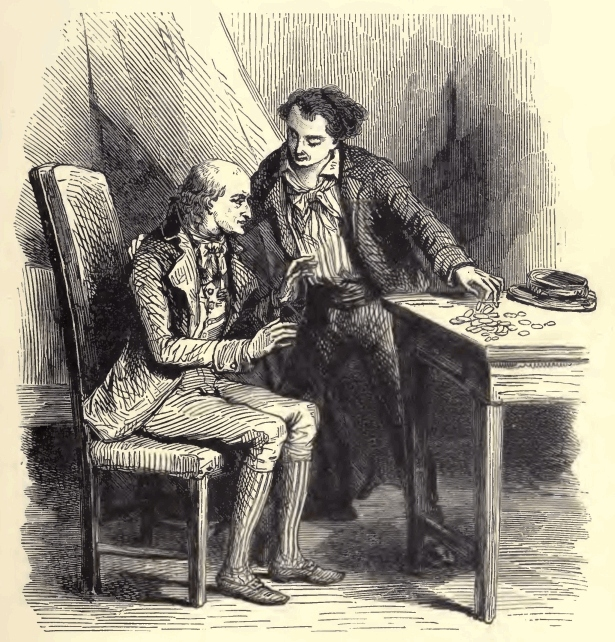
\includegraphics[width=\textwidth]{0035m.jpg}
\end{figure}

“Yes, here I am,” said the young man, “with a promising future and a
little money. Here, father, here!” he said, “take this—take it, and
send for something immediately.” And he emptied his pockets on the
table, the contents consisting of a dozen gold pieces, five or six
five-franc pieces, and some smaller coin. The countenance of old Dantès
brightened.

“Whom does this belong to?” he inquired.

“To me, to you, to us! Take it; buy some provisions; be happy, and
tomorrow we shall have more.”

“Gently, gently,” said the old man, with a smile; “and by your leave I
will use your purse moderately, for they would say, if they saw me buy
too many things at a time, that I had been obliged to await your
return, in order to be able to purchase them.”

“Do as you please; but, first of all, pray have a servant, father. I
will not have you left alone so long. I have some smuggled coffee and
most capital tobacco, in a small chest in the hold, which you shall
have tomorrow. But, hush, here comes somebody.”

“’Tis Caderousse, who has heard of your arrival, and no doubt comes to
congratulate you on your fortunate return.”

“Ah, lips that say one thing, while the heart thinks another,” murmured
Edmond. “But, never mind, he is a neighbor who has done us a service on
a time, so he’s welcome.”

As Edmond paused, the black and bearded head of Caderousse appeared at
the door. He was a man of twenty-five or six, and held a piece of
cloth, which, being a tailor, he was about to make into a coat-lining.

“What, is it you, Edmond, back again?” said he, with a broad
Marseillaise accent, and a grin that displayed his ivory-white teeth.

“Yes, as you see, neighbor Caderousse; and ready to be agreeable to you
in any and every way,” replied Dantès, but ill-concealing his coldness
under this cloak of civility.

“Thanks—thanks; but, fortunately, I do not want for anything; and it
chances that at times there are others who have need of me.” Dantès
made a gesture. “I do not allude to you, my boy. No!—no! I lent you
money, and you returned it; that’s like good neighbors, and we are
quits.”

“We are never quits with those who oblige us,” was Dantès’ reply; “for
when we do not owe them money, we owe them gratitude.”

“What’s the use of mentioning that? What is done is done. Let us talk
of your happy return, my boy. I had gone on the quay to match a piece
of mulberry cloth, when I met friend Danglars. ‘You at
Marseilles?’—‘Yes,’ says he.

“‘I thought you were at Smyrna.’—‘I was; but am now back again.’

“‘And where is the dear boy, our little Edmond?’

“‘Why, with his father, no doubt,’ replied Danglars. And so I came,”
added Caderousse, “as fast as I could to have the pleasure of shaking
hands with a friend.”

\begin{figure}[h]
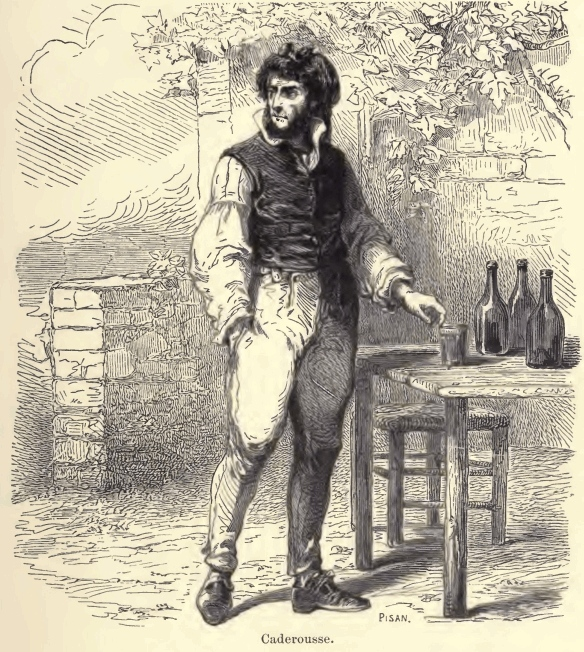
\includegraphics[width=\textwidth]{0037m.jpg}
\end{figure}

“Worthy Caderousse!” said the old man, “he is so much attached to us.”

“Yes, to be sure I am. I love and esteem you, because honest folks are
so rare. But it seems you have come back rich, my boy,” continued the
tailor, looking askance at the handful of gold and silver which Dantès
had thrown on the table.

The young man remarked the greedy glance which shone in the dark eyes
of his neighbor. “Eh,” he said, negligently, “this money is not mine. I
was expressing to my father my fears that he had wanted many things in
my absence, and to convince me he emptied his purse on the table. Come,
father” added Dantès, “put this money back in your box—unless neighbor
Caderousse wants anything, and in that case it is at his service.”

“No, my boy, no,” said Caderousse. “I am not in any want, thank God, my
living is suited to my means. Keep your money—keep it, I say;—one never
has too much;—but, at the same time, my boy, I am as much obliged by
your offer as if I took advantage of it.”

“It was offered with good will,” said Dantès.

“No doubt, my boy; no doubt. Well, you stand well with M. Morrel I
hear,—you insinuating dog, you!”

“M. Morrel has always been exceedingly kind to me,” replied Dantès.

“Then you were wrong to refuse to dine with him.”

“What, did you refuse to dine with him?” said old Dantès; “and did he
invite you to dine?”

“Yes, my dear father,” replied Edmond, smiling at his father’s
astonishment at the excessive honor paid to his son.

“And why did you refuse, my son?” inquired the old man.

“That I might the sooner see you again, my dear father,” replied the
young man. “I was most anxious to see you.”

“But it must have vexed M. Morrel, good, worthy man,” said Caderousse.
“And when you are looking forward to be captain, it was wrong to annoy
the owner.”

“But I explained to him the cause of my refusal,” replied Dantès, “and
I hope he fully understood it.”

“Yes, but to be captain one must do a little flattery to one’s
patrons.”

“I hope to be captain without that,” said Dantès.

“So much the better—so much the better! Nothing will give greater
pleasure to all your old friends; and I know one down there behind the
Saint Nicolas citadel who will not be sorry to hear it.”

“Mercédès?” said the old man.

“Yes, my dear father, and with your permission, now I have seen you,
and know you are well and have all you require, I will ask your consent
to go and pay a visit to the Catalans.”

“Go, my dear boy,” said old Dantès; “and Heaven bless you in your wife,
as it has blessed me in my son!”

“His wife!” said Caderousse; “why, how fast you go on, father Dantès;
she is not his wife yet, as it seems to me.”

“No, but according to all probability she soon will be,” replied
Edmond.

“Yes—yes,” said Caderousse; “but you were right to return as soon as
possible, my boy.”

“And why?”

“Because Mercédès is a very fine girl, and fine girls never lack
followers; she particularly has them by dozens.”

“Really?” answered Edmond, with a smile which had in it traces of
slight uneasiness.

\begin{figure}[h]
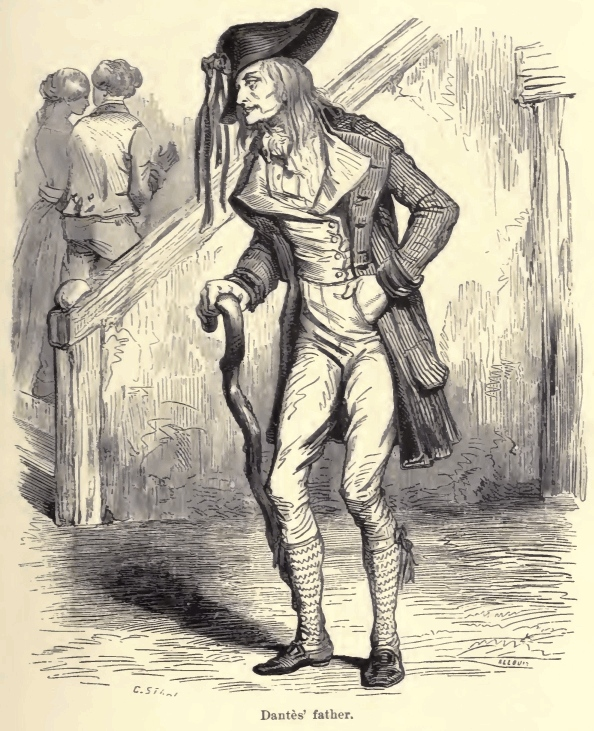
\includegraphics[width=\textwidth]{0039m.jpg}
\end{figure}

“Ah, yes,” continued Caderousse, “and capital offers, too; but you
know, you will be captain, and who could refuse you then?”

“Meaning to say,” replied Dantès, with a smile which but ill-concealed
his trouble, “that if I were not a captain——”

“Eh—eh!” said Caderousse, shaking his head.

“Come, come,” said the sailor, “I have a better opinion than you of
women in general, and of Mercédès in particular; and I am certain that,
captain or not, she will remain ever faithful to me.”

“So much the better—so much the better,” said Caderousse. “When one is
going to be married, there is nothing like implicit confidence; but
never mind that, my boy,—go and announce your arrival, and let her know
all your hopes and prospects.”

“I will go directly,” was Edmond’s reply; and, embracing his father,
and nodding to Caderousse, he left the apartment.

Caderousse lingered for a moment, then taking leave of old Dantès, he
went downstairs to rejoin Danglars, who awaited him at the corner of
the Rue Senac.

“Well,” said Danglars, “did you see him?”

“I have just left him,” answered Caderousse.

“Did he allude to his hope of being captain?”

“He spoke of it as a thing already decided.”

“Indeed!” said Danglars, “he is in too much hurry, it appears to me.”

“Why, it seems M. Morrel has promised him the thing.”

“So that he is quite elated about it?”

“Why, yes, he is actually insolent over the matter—has already offered
me his patronage, as if he were a grand personage, and proffered me a
loan of money, as though he were a banker.”

“Which you refused?”

“Most assuredly; although I might easily have accepted it, for it was I
who put into his hands the first silver he ever earned; but now M.
Dantès has no longer any occasion for assistance—he is about to become
a captain.”

“Pooh!” said Danglars, “he is not one yet.”

“\textit{Ma foi!} it will be as well if he is not,” answered Caderousse; “for
if he should be, there will be really no speaking to him.”

“If we choose,” replied Danglars, “he will remain what he is; and
perhaps become even less than he is.”

“What do you mean?”

“Nothing—I was speaking to myself. And is he still in love with the
Catalane?”

“Over head and ears; but, unless I am much mistaken, there will be a
storm in that quarter.”

\begin{figure}[h]
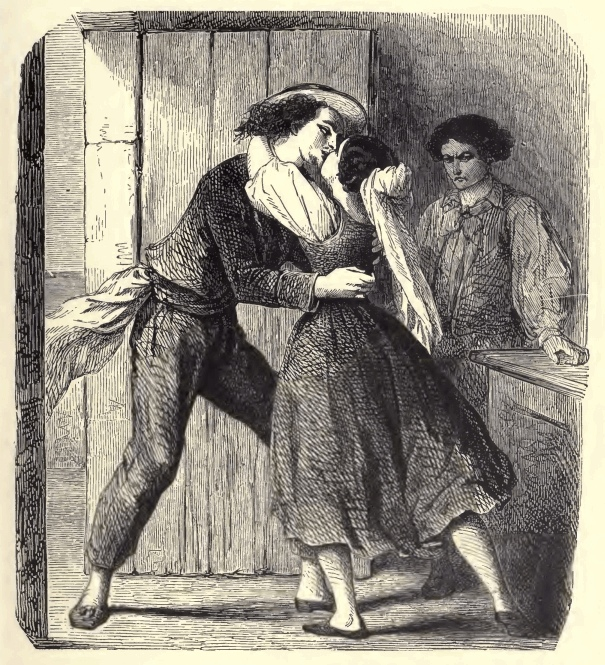
\includegraphics[width=\textwidth]{0041m.jpg}
\end{figure}

“Explain yourself.”

“Why should I?”

“It is more important than you think, perhaps. You do not like Dantès?”

“I never like upstarts.”

“Then tell me all you know about the Catalane.”

“I know nothing for certain; only I have seen things which induce me to
believe, as I told you, that the future captain will find some
annoyance in the vicinity of the Vieilles Infirmeries.”

“What have you seen?—come, tell me!”

“Well, every time I have seen Mercédès come into the city she has been
accompanied by a tall, strapping, black-eyed Catalan, with a red
complexion, brown skin, and fierce air, whom she calls cousin.”

“Really; and you think this cousin pays her attentions?”

“I only suppose so. What else can a strapping chap of twenty-one mean
with a fine wench of seventeen?”

“And you say that Dantès has gone to the Catalans?”

“He went before I came down.”

“Let us go the same way; we will stop at La Réserve, and we can drink a
glass of La Malgue, whilst we wait for news.”

“Come along,” said Caderousse; “but you pay the score.”

“Of course,” replied Danglars; and going quickly to the designated
place, they called for a bottle of wine, and two glasses.

Père Pamphile had seen Dantès pass not ten minutes before; and assured
that he was at the Catalans, they sat down under the budding foliage of
the planes and sycamores, in the branches of which the birds were
singing their welcome to one of the first days of spring.

\printpagenotes*
\chapter{The Catalans}

Beyond a bare, weather-worn wall, about a hundred paces from the spot
where the two friends sat looking and listening as they drank their
wine, was the village of the Catalans. Long ago this mysterious colony
quitted Spain, and settled on the tongue of land on which it is to this
day. Whence it came no one knew, and it spoke an unknown tongue. One of
its chiefs, who understood Provençal, begged the commune of Marseilles
to give them this bare and barren promontory, where, like the sailors
of old, they had run their boats ashore. The request was granted; and
three months afterwards, around the twelve or fifteen small vessels
which had brought these gypsies of the sea, a small village sprang up.
This village, constructed in a singular and picturesque manner, half
Moorish, half Spanish, still remains, and is inhabited by descendants
of the first comers, who speak the language of their fathers. For three
or four centuries they have remained upon this small promontory, on
which they had settled like a flight of seabirds, without mixing with
the Marseillaise population, intermarrying, and preserving their
original customs and the costume of their mother-country as they have
preserved its language.

Our readers will follow us along the only street of this little
village, and enter with us one of the houses, which is sunburned to the
beautiful dead-leaf color peculiar to the buildings of the country, and
within coated with whitewash, like a Spanish posada. A young and
beautiful girl, with hair as black as jet, her eyes as velvety as the
gazelle’s, was leaning with her back against the wainscot, rubbing in
her slender delicately moulded fingers a bunch of heath blossoms, the
flowers of which she was picking off and strewing on the floor; her
arms, bare to the elbow, brown, and modelled after those of the
Arlesian Venus, moved with a kind of restless impatience, and she
tapped the earth with her arched and supple foot, so as to display the
pure and full shape of her well-turned leg, in its red cotton, gray and
blue clocked, stocking. At three paces from her, seated in a chair
which he balanced on two legs, leaning his elbow on an old worm-eaten
table, was a tall young man of twenty, or two-and-twenty, who was
looking at her with an air in which vexation and uneasiness were
mingled. He questioned her with his eyes, but the firm and steady gaze
of the young girl controlled his look.

“You see, Mercédès,” said the young man, “here is Easter come round
again; tell me, is this the moment for a wedding?”

“I have answered you a hundred times, Fernand, and really you must be
very stupid to ask me again.”

“Well, repeat it,—repeat it, I beg of you, that I may at last believe
it! Tell me for the hundredth time that you refuse my love, which had
your mother’s sanction. Make me understand once for all that you are
trifling with my happiness, that my life or death are nothing to you.
Ah, to have dreamed for ten years of being your husband, Mercédès, and
to lose that hope, which was the only stay of my existence!”

“At least it was not I who ever encouraged you in that hope, Fernand,”
replied Mercédès; “you cannot reproach me with the slightest coquetry.
I have always said to you, ‘I love you as a brother; but do not ask
from me more than sisterly affection, for my heart is another’s.’ Is
not this true, Fernand?”

“Yes, that is very true, Mercédès,” replied the young man, “Yes, you
have been cruelly frank with me; but do you forget that it is among the
Catalans a sacred law to intermarry?”

\begin{figure}[ht]
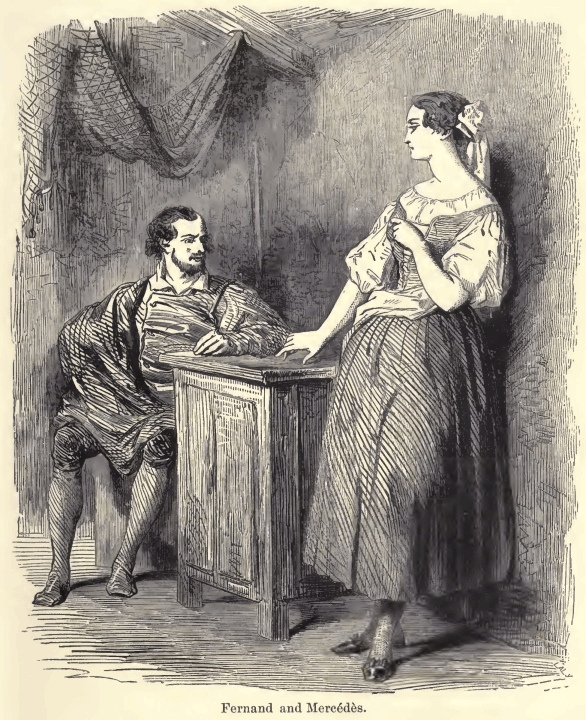
\includegraphics[width=\textwidth]{0045m.jpg}
\end{figure}

“You mistake, Fernand; it is not a law, but merely a custom, and, I
pray of you, do not cite this custom in your favor. You are included in
the conscription, Fernand, and are only at liberty on sufferance,
liable at any moment to be called upon to take up arms. Once a soldier,
what would you do with me, a poor orphan, forlorn, without fortune,
with nothing but a half-ruined hut and a few ragged nets, the miserable
inheritance left by my father to my mother, and by my mother to me? She
has been dead a year, and you know, Fernand, I have subsisted almost
entirely on public charity. Sometimes you pretend I am useful to you,
and that is an excuse to share with me the produce of your fishing, and
I accept it, Fernand, because you are the son of my father’s brother,
because we were brought up together, and still more because it would
give you so much pain if I refuse. But I feel very deeply that this
fish which I go and sell, and with the produce of which I buy the flax
I spin,—I feel very keenly, Fernand, that this is charity.”

“And if it were, Mercédès, poor and lone as you are, you suit me as
well as the daughter of the first shipowner or the richest banker of
Marseilles! What do such as we desire but a good wife and careful
housekeeper, and where can I look for these better than in you?”

“Fernand,” answered Mercédès, shaking her head, “a woman becomes a bad
manager, and who shall say she will remain an honest woman, when she
loves another man better than her husband? Rest content with my
friendship, for I say once more that is all I can promise, and I will
promise no more than I can bestow.”

“I understand,” replied Fernand, “you can endure your own wretchedness
patiently, but you are afraid to share mine. Well, Mercédès, beloved by
you, I would tempt fortune; you would bring me good luck, and I should
become rich. I could extend my occupation as a fisherman, might get a
place as clerk in a warehouse, and become in time a dealer myself.”

“You could do no such thing, Fernand; you are a soldier, and if you
remain at the Catalans it is because there is no war; so remain a
fisherman, and contented with my friendship, as I cannot give you
more.”

“Well, I will do better, Mercédès. I will be a sailor; instead of the
costume of our fathers, which you despise, I will wear a varnished hat,
a striped shirt, and a blue jacket, with an anchor on the buttons.
Would not that dress please you?”

“What do you mean?” asked Mercédès, with an angry glance,—“what do you
mean? I do not understand you?”

“I mean, Mercédès, that you are thus harsh and cruel with me, because
you are expecting someone who is thus attired; but perhaps he whom you
await is inconstant, or if he is not, the sea is so to him.”

“Fernand,” cried Mercédès, “I believed you were good-hearted, and I was
mistaken! Fernand, you are wicked to call to your aid jealousy and the
anger of God! Yes, I will not deny it, I do await, and I do love him of
whom you speak; and, if he does not return, instead of accusing him of
the inconstancy which you insinuate, I will tell you that he died
loving me and me only.” The young girl made a gesture of rage. “I
understand you, Fernand; you would be revenged on him because I do not
love you; you would cross your Catalan knife with his dirk. What end
would that answer? To lose you my friendship if he were conquered, and
see that friendship changed into hate if you were victor. Believe me,
to seek a quarrel with a man is a bad method of pleasing the woman who
loves that man. No, Fernand, you will not thus give way to evil
thoughts. Unable to have me for your wife, you will content yourself
with having me for your friend and sister; and besides,” she added, her
eyes troubled and moistened with tears, “wait, wait, Fernand; you said
just now that the sea was treacherous, and he has been gone four
months, and during these four months there have been some terrible
storms.”

Fernand made no reply, nor did he attempt to check the tears which
flowed down the cheeks of Mercédès, although for each of these tears he
would have shed his heart’s blood; but these tears flowed for another.
He arose, paced a while up and down the hut, and then, suddenly
stopping before Mercédès, with his eyes glowing and his hands
clenched,—“Say, Mercédès,” he said, “once for all, is this your final
determination?”

“I love Edmond Dantès,” the young girl calmly replied, “and none but
Edmond shall ever be my husband.”

“And you will always love him?”

“As long as I live.”

Fernand let fall his head like a defeated man, heaved a sigh that was
like a groan, and then suddenly looking her full in the face, with
clenched teeth and expanded nostrils, said,—“But if he is dead——”

“If he is dead, I shall die too.”

“If he has forgotten you——”

“Mercédès!” called a joyous voice from without,—“Mercédès!”

“Ah,” exclaimed the young girl, blushing with delight, and fairly
leaping in excess of love, “you see he has not forgotten me, for here
he is!” And rushing towards the door, she opened it, saying, “Here,
Edmond, here I am!”

Fernand, pale and trembling, drew back, like a traveller at the sight
of a serpent, and fell into a chair beside him. Edmond and Mercédès
were clasped in each other’s arms. The burning Marseilles sun, which
shot into the room through the open door, covered them with a flood of
light. At first they saw nothing around them. Their intense happiness
isolated them from all the rest of the world, and they only spoke in
broken words, which are the tokens of a joy so extreme that they seem
rather the expression of sorrow. Suddenly Edmond saw the gloomy, pale,
and threatening countenance of Fernand, as it was defined in the
shadow. By a movement for which he could scarcely account to himself,
the young Catalan placed his hand on the knife at his belt.

“Ah, your pardon,” said Dantès, frowning in his turn; “I did not
perceive that there were three of us.” Then, turning to Mercédès, he
inquired, “Who is this gentleman?”

“One who will be your best friend, Dantès, for he is my friend, my
cousin, my brother; it is Fernand—the man whom, after you, Edmond, I
love the best in the world. Do you not remember him?”

“Yes!” said Dantès, and without relinquishing Mercédès’ hand clasped in
one of his own, he extended the other to the Catalan with a cordial
air. But Fernand, instead of responding to this amiable gesture,
remained mute and trembling. Edmond then cast his eyes scrutinizingly
at the agitated and embarrassed Mercédès, and then again on the gloomy
and menacing Fernand. This look told him all, and his anger waxed hot.

“I did not know, when I came with such haste to you, that I was to meet
an enemy here.”

“An enemy!” cried Mercédès, with an angry look at her cousin. “An enemy
in my house, do you say, Edmond! If I believed that, I would place my
arm under yours and go with you to Marseilles, leaving the house to
return to it no more.”

Fernand’s eye darted lightning. “And should any misfortune occur to
you, dear Edmond,” she continued with the same calmness which proved to
Fernand that the young girl had read the very innermost depths of his
sinister thought, “if misfortune should occur to you, I would ascend
the highest point of the Cape de Morgiou and cast myself headlong from
it.”

Fernand became deadly pale. “But you are deceived, Edmond,” she
continued. “You have no enemy here—there is no one but Fernand, my
brother, who will grasp your hand as a devoted friend.”

And at these words the young girl fixed her imperious look on the
Catalan, who, as if fascinated by it, came slowly towards Edmond, and
offered him his hand. His hatred, like a powerless though furious wave,
was broken against the strong ascendancy which Mercédès exercised over
him. Scarcely, however, had he touched Edmond’s hand when he felt he
had done all he could do, and rushed hastily out of the house.

“Oh,” he exclaimed, running furiously and tearing his hair—“Oh, who
will deliver me from this man? Wretched—wretched that I am!”

“Hallo, Catalan! Hallo, Fernand! where are you running to?” exclaimed a
voice.

The young man stopped suddenly, looked around him, and perceived
Caderousse sitting at table with Danglars, under an arbor.

“Well”, said Caderousse, “why don’t you come? Are you really in such a
hurry that you have no time to pass the time of day with your friends?”

“Particularly when they have still a full bottle before them,” added
Danglars. Fernand looked at them both with a stupefied air, but did not
say a word.

“He seems besotted,” said Danglars, pushing Caderousse with his knee.
“Are we mistaken, and is Dantès triumphant in spite of all we have
believed?”

“Why, we must inquire into that,” was Caderousse’s reply; and turning
towards the young man, said, “Well, Catalan, can’t you make up your
mind?”

Fernand wiped away the perspiration steaming from his brow, and slowly
entered the arbor, whose shade seemed to restore somewhat of calmness
to his senses, and whose coolness somewhat of refreshment to his
exhausted body.

“Good-day,” said he. “You called me, didn’t you?” And he fell, rather
than sat down, on one of the seats which surrounded the table.

“I called you because you were running like a madman, and I was afraid
you would throw yourself into the sea,” said Caderousse, laughing.
“Why, when a man has friends, they are not only to offer him a glass of
wine, but, moreover, to prevent his swallowing three or four pints of
water unnecessarily!”

Fernand gave a groan, which resembled a sob, and dropped his head into
his hands, his elbows leaning on the table.

“Well, Fernand, I must say,” said Caderousse, beginning the
conversation, with that brutality of the common people in which
curiosity destroys all diplomacy, “you look uncommonly like a rejected
lover;” and he burst into a hoarse laugh.

“Bah!” said Danglars, “a lad of his make was not born to be unhappy in
love. You are laughing at him, Caderousse.”

“No,” he replied, “only hark how he sighs! Come, come, Fernand,” said
Caderousse, “hold up your head, and answer us. It’s not polite not to
reply to friends who ask news of your health.”

“My health is well enough,” said Fernand, clenching his hands without
raising his head.

“Ah, you see, Danglars,” said Caderousse, winking at his friend, “this
is how it is; Fernand, whom you see here, is a good and brave Catalan,
one of the best fishermen in Marseilles, and he is in love with a very
fine girl, named Mercédès; but it appears, unfortunately, that the fine
girl is in love with the mate of the \textit{Pharaon}; and as the \textit{Pharaon}
arrived today—why, you understand!”

“No; I do not understand,” said Danglars.

“Poor Fernand has been dismissed,” continued Caderousse.

“Well, and what then?” said Fernand, lifting up his head, and looking
at Caderousse like a man who looks for someone on whom to vent his
anger; “Mercédès is not accountable to any person, is she? Is she not
free to love whomsoever she will?”

“Oh, if you take it in that sense,” said Caderousse, “it is another
thing. But I thought you were a Catalan, and they told me the Catalans
were not men to allow themselves to be supplanted by a rival. It was
even told me that Fernand, especially, was terrible in his vengeance.”

Fernand smiled piteously. “A lover is never terrible,” he said.

“Poor fellow!” remarked Danglars, affecting to pity the young man from
the bottom of his heart. “Why, you see, he did not expect to see Dantès
return so suddenly—he thought he was dead, perhaps; or perchance
faithless! These things always come on us more severely when they come
suddenly.”

“Ah, \textit{ma foi}, under any circumstances!” said Caderousse, who drank as
he spoke, and on whom the fumes of the wine began to take
effect,—“under any circumstances Fernand is not the only person put out
by the fortunate arrival of Dantès; is he, Danglars?”

“No, you are right—and I should say that would bring him ill-luck.”

“Well, never mind,” answered Caderousse, pouring out a glass of wine
for Fernand, and filling his own for the eighth or ninth time, while
Danglars had merely sipped his. “Never mind—in the meantime he marries
Mercédès—the lovely Mercédès—at least he returns to do that.”

During this time Danglars fixed his piercing glance on the young man,
on whose heart Caderousse’s words fell like molten lead.

“And when is the wedding to be?” he asked.

“Oh, it is not yet fixed!” murmured Fernand.

“No, but it will be,” said Caderousse, “as surely as Dantès will be
captain of the \textit{Pharaon}—eh, Danglars?”

Danglars shuddered at this unexpected attack, and turned to Caderousse,
whose countenance he scrutinized, to try and detect whether the blow
was premeditated; but he read nothing but envy in a countenance already
rendered brutal and stupid by drunkenness.

“Well,” said he, filling the glasses, “let us drink to Captain Edmond
Dantès, husband of the beautiful Catalane!”

Caderousse raised his glass to his mouth with unsteady hand, and
swallowed the contents at a gulp. Fernand dashed his on the ground.

“Eh, eh, eh!” stammered Caderousse. “What do I see down there by the
wall, in the direction of the Catalans? Look, Fernand, your eyes are
better than mine. I believe I see double. You know wine is a deceiver;
but I should say it was two lovers walking side by side, and hand in
hand. Heaven forgive me, they do not know that we can see them, and
they are actually embracing!”

Danglars did not lose one pang that Fernand endured.

“Do you know them, Fernand?” he said.

“Yes,” was the reply, in a low voice. “It is Edmond and Mercédès!”

“Ah, see there, now!” said Caderousse; “and I did not recognize them!
Hallo, Dantès! hello, lovely damsel! Come this way, and let us know
when the wedding is to be, for Fernand here is so obstinate he will not
tell us.”

“Hold your tongue, will you?” said Danglars, pretending to restrain
Caderousse, who, with the tenacity of drunkards, leaned out of the
arbor. “Try to stand upright, and let the lovers make love without
interruption. See, look at Fernand, and follow his example; he is
well-behaved!”

\begin{figure}[h]
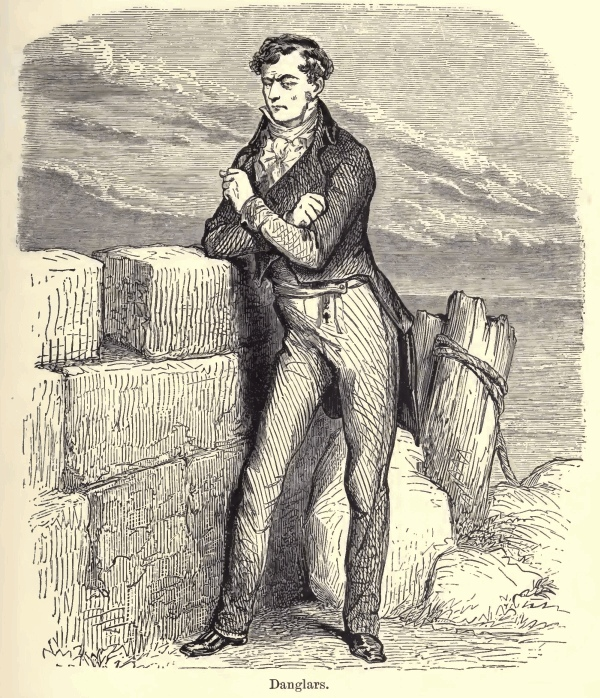
\includegraphics[width=\textwidth]{0051m.jpg}
\end{figure}

Fernand, probably excited beyond bearing, pricked by Danglars, as the
bull is by the bandilleros, was about to rush out; for he had risen
from his seat, and seemed to be collecting himself to dash headlong
upon his rival, when Mercédès, smiling and graceful, lifted up her
lovely head, and looked at them with her clear and bright eyes. At this
Fernand recollected her threat of dying if Edmond died, and dropped
again heavily on his seat. Danglars looked at the two men, one after
the other, the one brutalized by liquor, the other overwhelmed with
love.

“I shall get nothing from these fools,” he muttered; “and I am very
much afraid of being here between a drunkard and a coward. Here’s an
envious fellow making himself boozy on wine when he ought to be nursing
his wrath, and here is a fool who sees the woman he loves stolen from
under his nose and takes on like a big baby. Yet this Catalan has eyes
that glisten like those of the vengeful Spaniards, Sicilians, and
Calabrians, and the other has fists big enough to crush an ox at one
blow. Unquestionably, Edmond’s star is in the ascendant, and he will
marry the splendid girl—he will be captain, too, and laugh at us all,
unless”—a sinister smile passed over Danglars’ lips—“unless I take a
hand in the affair,” he added.

“Hallo!” continued Caderousse, half-rising, and with his fist on the
table, “hallo, Edmond! do you not see your friends, or are you too
proud to speak to them?”

“No, my dear fellow!” replied Dantès, “I am not proud, but I am happy,
and happiness blinds, I think, more than pride.”

“Ah, very well, that’s an explanation!” said Caderousse. “How do you
do, Madame Dantès?”

Mercédès courtesied gravely, and said—“That is not my name, and in my
country it bodes ill fortune, they say, to call a young girl by the
name of her betrothed before he becomes her husband. So call me
Mercédès, if you please.”

“We must excuse our worthy neighbor, Caderousse,” said Dantès, “he is
so easily mistaken.”

“So, then, the wedding is to take place immediately, M. Dantès,” said
Danglars, bowing to the young couple.

“As soon as possible, M. Danglars; today all preliminaries will be
arranged at my father’s, and tomorrow, or next day at latest, the
wedding festival here at La Réserve. My friends will be there, I hope;
that is to say, you are invited, M. Danglars, and you, Caderousse.”

“And Fernand,” said Caderousse with a chuckle; “Fernand, too, is
invited!”

“My wife’s brother is my brother,” said Edmond; “and we, Mercédès and
I, should be very sorry if he were absent at such a time.”

Fernand opened his mouth to reply, but his voice died on his lips, and
he could not utter a word.

“Today the preliminaries, tomorrow or next day the ceremony! You are in
a hurry, captain!”

“Danglars,” said Edmond, smiling, “I will say to you as Mercédès said
just now to Caderousse, ‘Do not give me a title which does not belong
to me’; that may bring me bad luck.”

“Your pardon,” replied Danglars, “I merely said you seemed in a hurry,
and we have lots of time; the \textit{Pharaon} cannot be under weigh again in
less than three months.”

“We are always in a hurry to be happy, M. Danglars; for when we have
suffered a long time, we have great difficulty in believing in good
fortune. But it is not selfishness alone that makes me thus in haste; I
must go to Paris.”

“Ah, really?—to Paris! and will it be the first time you have ever been
there, Dantès?”

“Yes.”

“Have you business there?”

“Not of my own; the last commission of poor Captain Leclere; you know
to what I allude, Danglars—it is sacred. Besides, I shall only take the
time to go and return.”

“Yes, yes, I understand,” said Danglars, and then in a low tone, he
added, “To Paris, no doubt to deliver the letter which the grand
marshal gave him. Ah, this letter gives me an idea—a capital idea! Ah;
Dantès, my friend, you are not yet registered number one on board the
good ship \textit{Pharaon};” then turning towards Edmond, who was walking
away, “A pleasant journey,” he cried.

“Thank you,” said Edmond with a friendly nod, and the two lovers
continued on their way, as calm and joyous as if they were the very
elect of heaven.

\printpagenotes*
\chapter{Conspiracy}

Danglars followed Edmond and Mercédès with his eyes until the two
lovers disappeared behind one of the angles of Fort Saint Nicolas;
then, turning round, he perceived Fernand, who had fallen, pale and
trembling, into his chair, while Caderousse stammered out the words of
a drinking-song.

“Well, my dear sir,” said Danglars to Fernand, “here is a marriage
which does not appear to make everybody happy.”

“It drives me to despair,” said Fernand.

“Do you, then, love Mercédès?”

“I adore her!”

“For long?”

“As long as I have known her—always.”

“And you sit there, tearing your hair, instead of seeking to remedy
your condition; I did not think that was the way of your people.”

“What would you have me do?” said Fernand.

“How do I know? Is it my affair? I am not in love with Mademoiselle
Mercédès; but for you—in the words of the gospel, seek, and you shall
find.”

“I have found already.”

“What?”

“I would stab the man, but the woman told me that if any misfortune
happened to her betrothed, she would kill herself.”

“Pooh! Women say those things, but never do them.”

“You do not know Mercédès; what she threatens she will do.”

“Idiot!” muttered Danglars; “whether she kill herself or not, what
matter, provided Dantès is not captain?”

“Before Mercédès should die,” replied Fernand, with the accents of
unshaken resolution, “I would die myself!”

“That’s what I call love!” said Caderousse with a voice more tipsy than
ever. “That’s love, or I don’t know what love is.”

“Come,” said Danglars, “you appear to me a good sort of fellow, and
hang me, I should like to help you, but——”

“Yes,” said Caderousse, “but how?”

“My dear fellow,” replied Danglars, “you are three parts drunk; finish
the bottle, and you will be completely so. Drink then, and do not
meddle with what we are discussing, for that requires all one’s wit and
cool judgment.”

“I—drunk!” said Caderousse; “well that’s a good one! I could drink four
more such bottles; they are no bigger than cologne flasks. Père
Pamphile, more wine!”

And Caderousse rattled his glass upon the table.

“You were saying, sir——” said Fernand, awaiting with great anxiety the
end of this interrupted remark.

“What was I saying? I forget. This drunken Caderousse has made me lose
the thread of my sentence.”

“Drunk, if you like; so much the worse for those who fear wine, for it
is because they have bad thoughts which they are afraid the liquor will
extract from their hearts;” and Caderousse began to sing the two last
lines of a song very popular at the time:

\hspace{1cm}{\small ‘Tous les méchants sont buveurs d’eau;

\hspace{1cm}C’est bien prouvé par le déluge.’}\footnote[1]{“The wicked
are great drinkers of water; As the flood proved once for all.” }

“You said, sir, you would like to help me, but——”

“Yes; but I added, to help you it would be sufficient that Dantès did
not marry her you love; and the marriage may easily be thwarted,
methinks, and yet Dantès need not die.”

“Death alone can separate them,” remarked Fernand.

“You talk like a noodle, my friend,” said Caderousse; “and here is
Danglars, who is a wide-awake, clever, deep fellow, who will prove to
you that you are wrong. Prove it, Danglars. I have answered for you.
Say there is no need why Dantès should die; it would, indeed, be a pity
he should. Dantès is a good fellow; I like Dantès. Dantès, your
health.”

Fernand rose impatiently. “Let him run on,” said Danglars, restraining
the young man; “drunk as he is, he is not much out in what he says.
Absence severs as well as death, and if the walls of a prison were
between Edmond and Mercédès they would be as effectually separated as
if he lay under a tombstone.”

\begin{figure}[ht]
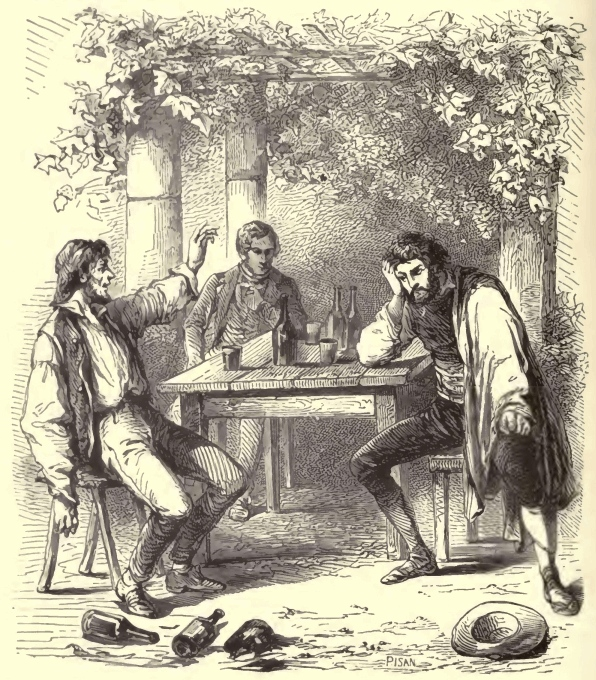
\includegraphics[width=\textwidth]{0056m.jpg}
\end{figure}

“Yes; but one gets out of prison,” said Caderousse, who, with what
sense was left him, listened eagerly to the conversation, “and when one
gets out and one’s name is Edmond Dantès, one seeks revenge——”

“What matters that?” muttered Fernand.

“And why, I should like to know,” persisted Caderousse, “should they
put Dantès in prison? he has neither robbed, nor killed, nor murdered.”

“Hold your tongue!” said Danglars.

“I won’t hold my tongue!” replied Caderousse; “I say I want to know why
they should put Dantès in prison; I like Dantès; Dantès, your health!”
and he swallowed another glass of wine.

\begin{figure}[ht]
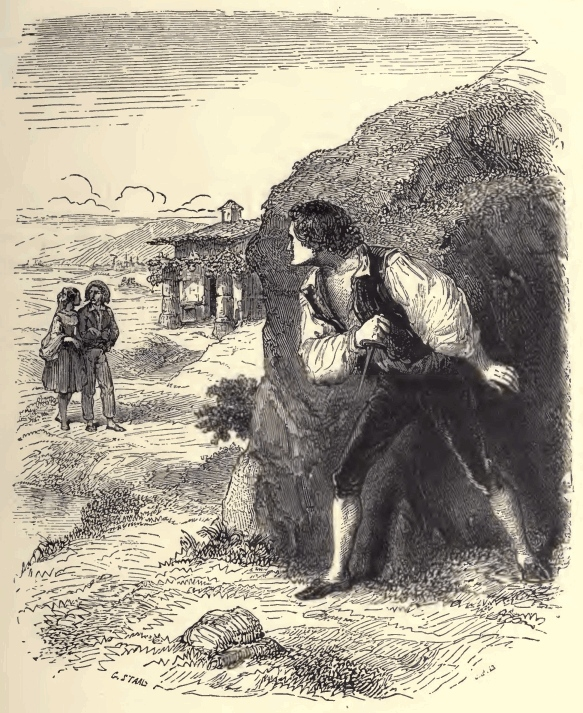
\includegraphics[width=\textwidth]{0057m.jpg}
\end{figure}

Danglars saw in the muddled look of the tailor the progress of his
intoxication, and turning towards Fernand, said, “Well, you understand
there is no need to kill him.”

“Certainly not, if, as you said just now, you have the means of having
Dantès arrested. Have you that means?”

“It is to be found for the searching. But why should I meddle in the
matter? it is no affair of mine.”

“I know not why you meddle,” said Fernand, seizing his arm; “but this I
know, you have some motive of personal hatred against Dantès, for he
who himself hates is never mistaken in the sentiments of others.”

“I! motives of hatred against Dantès? None, on my word! I saw you were
unhappy, and your unhappiness interested me; that’s all; but since you
believe I act for my own account, adieu, my dear friend, get out of the
affair as best you may;” and Danglars rose as if he meant to depart.

“No, no,” said Fernand, restraining him, “stay! It is of very little
consequence to me at the end of the matter whether you have any angry
feeling or not against Dantès. I hate him! I confess it openly. Do you
find the means, I will execute it, provided it is not to kill the man,
for Mercédès has declared she will kill herself if Dantès is killed.”

Caderousse, who had let his head drop on the table, now raised it, and
looking at Fernand with his dull and fishy eyes, he said, “Kill Dantès!
who talks of killing Dantès? I won’t have him killed—I won’t! He’s my
friend, and this morning offered to share his money with me, as I
shared mine with him. I won’t have Dantès killed—I won’t!”

“And who has said a word about killing him, muddlehead?” replied
Danglars. “We were merely joking; drink to his health,” he added,
filling Caderousse’s glass, “and do not interfere with us.”

“Yes, yes, Dantès’ good health!” said Caderousse, emptying his glass,
“here’s to his health! his health—hurrah!”

“But the means—the means?” said Fernand.

“Have you not hit upon any?” asked Danglars.

“No!—you undertook to do so.”

“True,” replied Danglars; “the French have the superiority over the
Spaniards, that the Spaniards ruminate, while the French invent.”

“Do you invent, then,” said Fernand impatiently.

“Waiter,” said Danglars, “pen, ink, and paper.”

“Pen, ink, and paper,” muttered Fernand.

“Yes; I am a supercargo; pen, ink, and paper are my tools, and without
my tools I am fit for nothing.”

“Pen, ink, and paper, then,” called Fernand loudly.

“There’s what you want on that table,” said the waiter.

“Bring them here.” The waiter did as he was desired.

\begin{figure}[h]
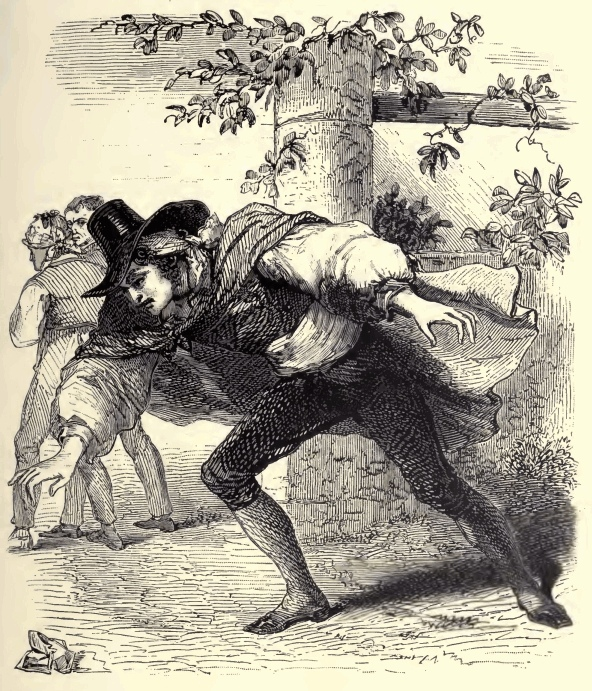
\includegraphics[width=\textwidth]{0059m.jpg}
\end{figure}

“When one thinks,” said Caderousse, letting his hand drop on the paper,
“there is here wherewithal to kill a man more sure than if we waited at
the corner of a wood to assassinate him! I have always had more dread
of a pen, a bottle of ink, and a sheet of paper, than of a sword or
pistol.”

“The fellow is not so drunk as he appears to be,” said Danglars. “Give
him some more wine, Fernand.” Fernand filled Caderousse’s glass, who,
like the confirmed toper he was, lifted his hand from the paper and
seized the glass.

The Catalan watched him until Caderousse, almost overcome by this fresh
assault on his senses, rested, or rather dropped, his glass upon the
table.

“Well!” resumed the Catalan, as he saw the final glimmer of
Caderousse’s reason vanishing before the last glass of wine.

“Well, then, I should say, for instance,” resumed Danglars, “that if
after a voyage such as Dantès has just made, in which he touched at the
Island of Elba, someone were to denounce him to the king’s procureur as
a Bonapartist agent——”

“I will denounce him!” exclaimed the young man hastily.

“Yes, but they will make you then sign your declaration, and confront
you with him you have denounced; I will supply you with the means of
supporting your accusation, for I know the fact well. But Dantès cannot
remain forever in prison, and one day or other he will leave it, and
the day when he comes out, woe betide him who was the cause of his
incarceration!”

“Oh, I should wish nothing better than that he would come and seek a
quarrel with me.”

“Yes, and Mercédès! Mercédès, who will detest you if you have only the
misfortune to scratch the skin of her dearly beloved Edmond!”

“True!” said Fernand.

“No, no,” continued Danglars; “if we resolve on such a step, it would
be much better to take, as I now do, this pen, dip it into this ink,
and write with the left hand (that the writing may not be recognized)
the denunciation we propose.” And Danglars, uniting practice with
theory, wrote with his left hand, and in a writing reversed from his
usual style, and totally unlike it, the following lines, which he
handed to Fernand, and which Fernand read in an undertone:

“The honorable, the king’s attorney, is informed by a friend of the
throne and religion, that one Edmond Dantès, mate of the ship
\textit{Pharaon}, arrived this morning from Smyrna, after having touched at
Naples and Porto-Ferrajo, has been intrusted by Murat with a letter for
the usurper, and by the usurper with a letter for the Bonapartist
committee in Paris. Proof of this crime will be found on arresting him,
for the letter will be found upon him, or at his father’s, or in his
cabin on board the \textit{Pharaon}.”

“Very good,” resumed Danglars; “now your revenge looks like common
sense, for in no way can it revert to yourself, and the matter will
thus work its own way; there is nothing to do now but fold the letter
as I am doing, and write upon it, ‘To the king’s attorney,’ and that’s
all settled.” And Danglars wrote the address as he spoke.

“Yes, and that’s all settled!” exclaimed Caderousse, who, by a last
effort of intellect, had followed the reading of the letter, and
instinctively comprehended all the misery which such a denunciation
must entail. “Yes, and that’s all settled; only it will be an infamous
shame;” and he stretched out his hand to reach the letter.

“Yes,” said Danglars, taking it from beyond his reach; “and as what I
say and do is merely in jest, and I, amongst the first and foremost,
should be sorry if anything happened to Dantès—the worthy Dantès—look
here!” And taking the letter, he squeezed it up in his hands and threw
it into a corner of the arbor.

“All right!” said Caderousse. “Dantès is my friend, and I won’t have
him ill-used.”

“And who thinks of using him ill? Certainly neither I nor Fernand,”
said Danglars, rising and looking at the young man, who still remained
seated, but whose eye was fixed on the denunciatory sheet of paper
flung into the corner.

“In this case,” replied Caderousse, “let’s have some more wine. I wish
to drink to the health of Edmond and the lovely Mercédès.”

“You have had too much already, drunkard,” said Danglars; “and if you
continue, you will be compelled to sleep here, because unable to stand
on your legs.”

“I?” said Caderousse, rising with all the offended dignity of a drunken
man, “I can’t keep on my legs? Why, I’ll wager I can go up into the
belfry of the Accoules, and without staggering, too!”

“Done!” said Danglars, “I’ll take your bet; but tomorrow—today it is
time to return. Give me your arm, and let us go.”

“Very well, let us go,” said Caderousse; “but I don’t want your arm at
all. Come, Fernand, won’t you return to Marseilles with us?”

“No,” said Fernand; “I shall return to the Catalans.”

“You’re wrong. Come with us to Marseilles—come along.”

“I will not.”

“What do you mean? you will not? Well, just as you like, my prince;
there’s liberty for all the world. Come along, Danglars, and let the
young gentleman return to the Catalans if he chooses.”

Danglars took advantage of Caderousse’s temper at the moment, to take
him off towards Marseilles by the Porte Saint-Victor, staggering as he
went.

When they had advanced about twenty yards, Danglars looked back and saw
Fernand stoop, pick up the crumpled paper, and putting it into his
pocket then rush out of the arbor towards Pillon.

“Well,” said Caderousse, “why, what a lie he told! He said he was going
to the Catalans, and he is going to the city. Hallo, Fernand! You are
coming, my boy!”

“Oh, you don’t see straight,” said Danglars; “he’s gone right by the
road to the Vieilles Infirmeries.”

“Well,” said Caderousse, “I should have sworn that he turned to the
right—how treacherous wine is!”

“Come, come,” said Danglars to himself, “now the thing is at work and
it will effect its purpose unassisted.”

\printpagenotes*
\chapter{The Marriage Feast}

The morning’s sun rose clear and resplendent, touching the foamy waves
into a network of ruby-tinted light.

The feast had been made ready on the second floor at La Réserve, with
whose arbor the reader is already familiar. The apartment destined for
the purpose was spacious and lighted by a number of windows, over each
of which was written in golden letters for some inexplicable reason the
name of one of the principal cities of France; beneath these windows a
wooden balcony extended the entire length of the house. And although
the entertainment was fixed for twelve o’clock, an hour previous to
that time the balcony was filled with impatient and expectant guests,
consisting of the favored part of the crew of the \textit{Pharaon}, and other
personal friends of the bridegroom, the whole of whom had arrayed
themselves in their choicest costumes, in order to do greater honor to
the occasion.

Various rumors were afloat to the effect that the owners of the
\textit{Pharaon} had promised to attend the nuptial feast; but all seemed
unanimous in doubting that an act of such rare and exceeding
condescension could possibly be intended.

Danglars, however, who now made his appearance, accompanied by
Caderousse, effectually confirmed the report, stating that he had
recently conversed with M. Morrel, who had himself assured him of his
intention to dine at La Réserve.

In fact, a moment later M. Morrel appeared and was saluted with an
enthusiastic burst of applause from the crew of the \textit{Pharaon}, who
hailed the visit of the shipowner as a sure indication that the man
whose wedding feast he thus delighted to honor would ere long be first
in command of the ship; and as Dantès was universally beloved on board
his vessel, the sailors put no restraint on their tumultuous joy at
finding that the opinion and choice of their superiors so exactly
coincided with their own.

With the entrance of M. Morrel, Danglars and Caderousse were despatched
in search of the bridegroom to convey to him the intelligence of the
arrival of the important personage whose coming had created such a
lively sensation, and to beseech him to make haste.

Danglars and Caderousse set off upon their errand at full speed; but
ere they had gone many steps they perceived a group advancing towards
them, composed of the betrothed pair, a party of young girls in
attendance on the bride, by whose side walked Dantès’ father; the whole
brought up by Fernand, whose lips wore their usual sinister smile.

Neither Mercédès nor Edmond observed the strange expression of his
countenance; they were so happy that they were conscious only of the
sunshine and the presence of each other.

Having acquitted themselves of their errand, and exchanged a hearty
shake of the hand with Edmond, Danglars and Caderousse took their
places beside Fernand and old Dantès,—the latter of whom attracted
universal notice.

The old man was attired in a suit of glistening watered silk, trimmed
with steel buttons, beautifully cut and polished. His thin but wiry
legs were arrayed in a pair of richly embroidered clocked stockings,
evidently of English manufacture, while from his three-cornered hat
depended a long streaming knot of white and blue ribbons. Thus he came
along, supporting himself on a curiously carved stick, his aged
countenance lit up with happiness, looking for all the world like one
of the aged dandies of 1796, parading the newly opened gardens of the
Luxembourg and Tuileries.

Beside him glided Caderousse, whose desire to partake of the good
things provided for the wedding party had induced him to become
reconciled to the Dantès, father and son, although there still lingered
in his mind a faint and unperfect recollection of the events of the
preceding night; just as the brain retains on waking in the morning the
dim and misty outline of a dream.

\begin{figure}[ht]
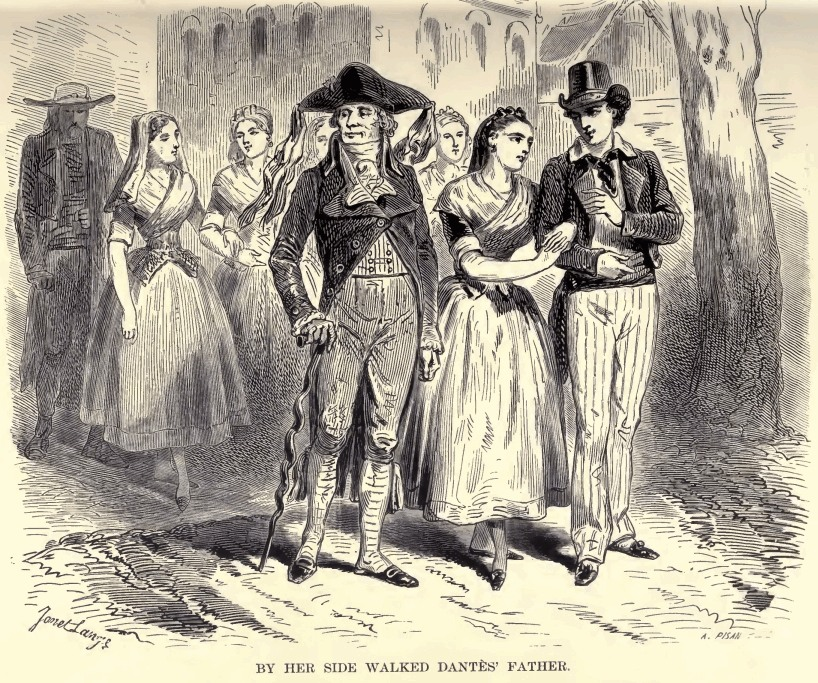
\includegraphics[width=\textwidth]{0065m.jpg}
\end{figure}

As Danglars approached the disappointed lover, he cast on him a look of
deep meaning, while Fernand, as he slowly paced behind the happy pair,
who seemed, in their own unmixed content, to have entirely forgotten
that such a being as himself existed, was pale and abstracted;
occasionally, however, a deep flush would overspread his countenance,
and a nervous contraction distort his features, while, with an agitated
and restless gaze, he would glance in the direction of Marseilles, like
one who either anticipated or foresaw some great and important event.

Dantès himself was simply, but becomingly, clad in the dress peculiar
to the merchant service—a costume somewhat between a military and a
civil garb; and with his fine countenance, radiant with joy and
happiness, a more perfect specimen of manly beauty could scarcely be
imagined.

Lovely as the Greek girls of Cyprus or Chios, Mercédès boasted the same
bright flashing eyes of jet, and ripe, round, coral lips. She moved
with the light, free step of an Arlesienne or an Andalusian. One more
practiced in the arts of great cities would have hid her blushes
beneath a veil, or, at least, have cast down her thickly fringed
lashes, so as to have concealed the liquid lustre of her animated eyes;
but, on the contrary, the delighted girl looked around her with a smile
that seemed to say: “If you are my friends, rejoice with me, for I am
very happy.”

As soon as the bridal party came in sight of La Réserve, M. Morrel
descended and came forth to meet it, followed by the soldiers and
sailors there assembled, to whom he had repeated the promise already
given, that Dantès should be the successor to the late Captain Leclere.
Edmond, at the approach of his patron, respectfully placed the arm of
his affianced bride within that of M. Morrel, who, forthwith conducting
her up the flight of wooden steps leading to the chamber in which the
feast was prepared, was gayly followed by the guests, beneath whose
heavy tread the slight structure creaked and groaned for the space of
several minutes.

“Father,” said Mercédès, stopping when she had reached the centre of
the table, “sit, I pray you, on my right hand; on my left I will place
him who has ever been as a brother to me,” pointing with a soft and
gentle smile to Fernand; but her words and look seemed to inflict the
direst torture on him, for his lips became ghastly pale, and even
beneath the dark hue of his complexion the blood might be seen
retreating as though some sudden pang drove it back to the heart.

During this time, Dantès, at the opposite side of the table, had been
occupied in similarly placing his most honored guests. M. Morrel was
seated at his right hand, Danglars at his left; while, at a sign from
Edmond, the rest of the company ranged themselves as they found it most
agreeable.

Then they began to pass around the dusky, piquant, Arlesian sausages,
and lobsters in their dazzling red cuirasses, prawns of large size and
brilliant color, the echinus with its prickly outside and dainty morsel
within, the clovis, esteemed by the epicures of the South as more than
rivalling the exquisite flavor of the oyster, North. All the
delicacies, in fact, that are cast up by the wash of waters on the
sandy beach, and styled by the grateful fishermen “fruits of the sea.”

“A pretty silence truly!” said the old father of the bridegroom, as he
carried to his lips a glass of wine of the hue and brightness of the
topaz, and which had just been placed before Mercédès herself. “Now,
would anybody think that this room contained a happy, merry party, who
desire nothing better than to laugh and dance the hours away?”

“Ah,” sighed Caderousse, “a man cannot always feel happy because he is
about to be married.”

“The truth is,” replied Dantès, “that I am too happy for noisy mirth;
if that is what you meant by your observation, my worthy friend, you
are right; joy takes a strange effect at times, it seems to oppress us
almost the same as sorrow.”

Danglars looked towards Fernand, whose excitable nature received and
betrayed each fresh impression.

“Why, what ails you?” asked he of Edmond. “Do you fear any approaching
evil? I should say that you were the happiest man alive at this
instant.”

“And that is the very thing that alarms me,” returned Dantès. “Man does
not appear to me to be intended to enjoy felicity so unmixed; happiness
is like the enchanted palaces we read of in our childhood, where
fierce, fiery dragons defend the entrance and approach; and monsters of
all shapes and kinds, requiring to be overcome ere victory is ours. I
own that I am lost in wonder to find myself promoted to an honor of
which I feel myself unworthy—that of being the husband of Mercédès.”

“Nay, nay!” cried Caderousse, smiling, “you have not attained that
honor yet. Mercédès is not yet your wife. Just assume the tone and
manner of a husband, and see how she will remind you that your hour is
not yet come!”

The bride blushed, while Fernand, restless and uneasy, seemed to start
at every fresh sound, and from time to time wiped away the large drops
of perspiration that gathered on his brow.

“Well, never mind that, neighbor Caderousse; it is not worthwhile to
contradict me for such a trifle as that. ’Tis true that Mercédès is not
actually my wife; but,” added he, drawing out his watch, “in an hour
and a half she will be.”

A general exclamation of surprise ran round the table, with the
exception of the elder Dantès, whose laugh displayed the still perfect
beauty of his large white teeth. Mercédès looked pleased and gratified,
while Fernand grasped the handle of his knife with a convulsive clutch.

“In an hour?” inquired Danglars, turning pale. “How is that, my
friend?”

“Why, thus it is,” replied Dantès. “Thanks to the influence of M.
Morrel, to whom, next to my father, I owe every blessing I enjoy, every
difficulty has been removed. We have purchased permission to waive the
usual delay; and at half-past two o’clock the Mayor of Marseilles will
be waiting for us at the city hall. Now, as a quarter-past one has
already struck, I do not consider I have asserted too much in saying,
that, in another hour and thirty minutes Mercédès will have become
Madame Dantès.”

\begin{figure}[ht]
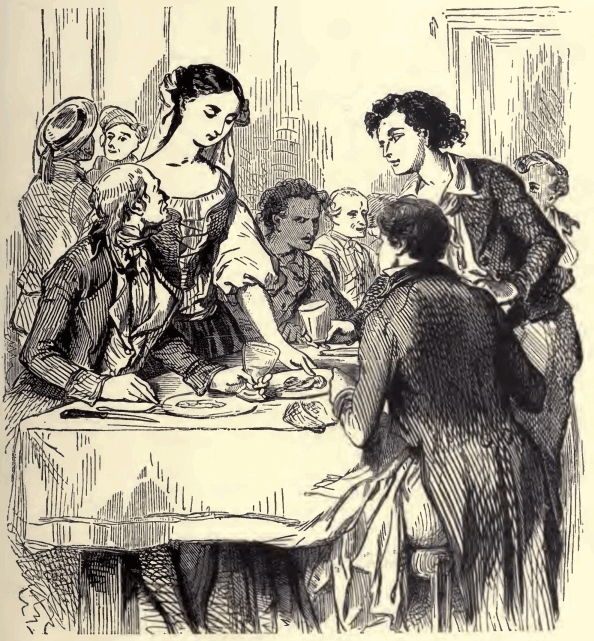
\includegraphics[width=\textwidth]{0069m.jpg}
\end{figure}

Fernand closed his eyes, a burning sensation passed across his brow,
and he was compelled to support himself by the table to prevent his
falling from his chair; but in spite of all his efforts, he could not
refrain from uttering a deep groan, which, however, was lost amid the
noisy felicitations of the company.

“Upon my word,” cried the old man, “you make short work of this kind of
affair. Arrived here only yesterday morning, and married today at three
o’clock! Commend me to a sailor for going the quick way to work!”

“But,” asked Danglars, in a timid tone, “how did you manage about the
other formalities—the contract—the settlement?”

“The contract,” answered Dantès, laughingly, “it didn’t take long to
fix that. Mercédès has no fortune; I have none to settle on her. So,
you see, our papers were quickly written out, and certainly do not come
very expensive.” This joke elicited a fresh burst of applause.

“So that what we presumed to be merely the betrothal feast turns out to
be the actual wedding dinner!” said Danglars.

“No, no,” answered Dantès; “don’t imagine I am going to put you off in
that shabby manner. Tomorrow morning I start for Paris; four days to
go, and the same to return, with one day to discharge the commission
entrusted to me, is all the time I shall be absent. I shall be back
here by the first of March, and on the second I give my real marriage
feast.”

This prospect of fresh festivity redoubled the hilarity of the guests
to such a degree, that the elder Dantès, who, at the commencement of
the repast, had commented upon the silence that prevailed, now found it
difficult, amid the general din of voices, to obtain a moment’s
tranquillity in which to drink to the health and prosperity of the
bride and bridegroom.

Dantès, perceiving the affectionate eagerness of his father, responded
by a look of grateful pleasure; while Mercédès glanced at the clock and
made an expressive gesture to Edmond.

Around the table reigned that noisy hilarity which usually prevails at
such a time among people sufficiently free from the demands of social
position not to feel the trammels of etiquette. Such as at the
commencement of the repast had not been able to seat themselves
according to their inclination rose unceremoniously, and sought out
more agreeable companions. Everybody talked at once, without waiting
for a reply and each one seemed to be contented with expressing his or
her own thoughts.

Fernand’s paleness appeared to have communicated itself to Danglars. As
for Fernand himself, he seemed to be enduring the tortures of the
damned; unable to rest, he was among the first to quit the table, and,
as though seeking to avoid the hilarious mirth that rose in such
deafening sounds, he continued, in utter silence, to pace the farther
end of the salon.

Caderousse approached him just as Danglars, whom Fernand seemed most
anxious to avoid, had joined him in a corner of the room.

“Upon my word,” said Caderousse, from whose mind the friendly treatment
of Dantès, united with the effect of the excellent wine he had partaken
of, had effaced every feeling of envy or jealousy at Dantès’ good
fortune,—“upon my word, Dantès is a downright good fellow, and when I
see him sitting there beside his pretty wife that is so soon to be. I
cannot help thinking it would have been a great pity to have served him
that trick you were planning yesterday.”

“Oh, there was no harm meant,” answered Danglars; “at first I certainly
did feel somewhat uneasy as to what Fernand might be tempted to do; but
when I saw how completely he had mastered his feelings, even so far as
to become one of his rival’s attendants, I knew there was no further
cause for apprehension.” Caderousse looked full at Fernand—he was
ghastly pale.

“Certainly,” continued Danglars, “the sacrifice was no trifling one,
when the beauty of the bride is concerned. Upon my soul, that future
captain of mine is a lucky dog! Gad! I only wish he would let me take
his place.”

“Shall we not set forth?” asked the sweet, silvery voice of Mercédès;
“two o’clock has just struck, and you know we are expected in a quarter
of an hour.”

\begin{figure}[ht]
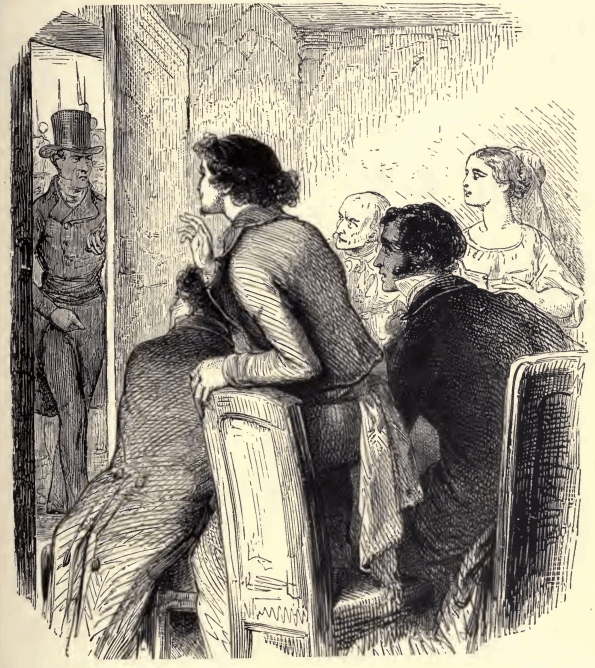
\includegraphics[width=\textwidth]{0071m.jpg}
\end{figure}

“To be sure!—to be sure!” cried Dantès, eagerly quitting the table;
“let us go directly!”

His words were re-echoed by the whole party, with vociferous cheers.

At this moment Danglars, who had been incessantly observing every
change in Fernand’s look and manner, saw him stagger and fall back,
with an almost convulsive spasm, against a seat placed near one of the
open windows. At the same instant his ear caught a sort of indistinct
sound on the stairs, followed by the measured tread of soldiery, with
the clanking of swords and military accoutrements; then came a hum and
buzz as of many voices, so as to deaden even the noisy mirth of the
bridal party, among whom a vague feeling of curiosity and apprehension
quelled every disposition to talk, and almost instantaneously the most
deathlike stillness prevailed.

The sounds drew nearer. Three blows were struck upon the panel of the
door. The company looked at each other in consternation.

“I demand admittance,” said a loud voice outside the room, “in the name
of the law!” As no attempt was made to prevent it, the door was opened,
and a magistrate, wearing his official scarf, presented himself,
followed by four soldiers and a corporal. Uneasiness now yielded to the
most extreme dread on the part of those present.

“May I venture to inquire the reason of this unexpected visit?” said M.
Morrel, addressing the magistrate, whom he evidently knew; “there is
doubtless some mistake easily explained.”

“If it be so,” replied the magistrate, “rely upon every reparation
being made; meanwhile, I am the bearer of an order of arrest, and
although I most reluctantly perform the task assigned me, it must,
nevertheless, be fulfilled. Who among the persons here assembled
answers to the name of Edmond Dantès?”

Every eye was turned towards the young man who, spite of the agitation
he could not but feel, advanced with dignity, and said, in a firm
voice:

“I am he; what is your pleasure with me?”

“Edmond Dantès,” replied the magistrate, “I arrest you in the name of
the law!”

“Me!” repeated Edmond, slightly changing color, “and wherefore, I
pray?”

“I cannot inform you, but you will be duly acquainted with the reasons
that have rendered such a step necessary at the preliminary
examination.”

M. Morrel felt that further resistance or remonstrance was useless. He
saw before him an officer delegated to enforce the law, and perfectly
well knew that it would be as unavailing to seek pity from a magistrate
decked with his official scarf, as to address a petition to some cold
marble effigy. Old Dantès, however, sprang forward. There are
situations which the heart of a father or a mother cannot be made to
understand. He prayed and supplicated in terms so moving, that even the
officer was touched, and, although firm in his duty, he kindly said,
“My worthy friend, let me beg of you to calm your apprehensions. Your
son has probably neglected some prescribed form or attention in
registering his cargo, and it is more than probable he will be set at
liberty directly he has given the information required, whether
touching the health of his crew, or the value of his freight.”

“What is the meaning of all this?” inquired Caderousse, frowningly, of
Danglars, who had assumed an air of utter surprise.

\begin{figure}[h]
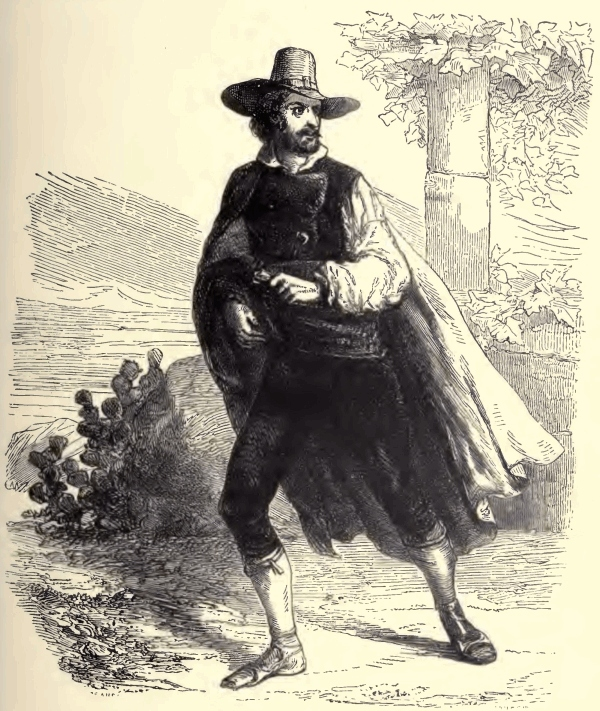
\includegraphics[width=\textwidth]{0073m.jpg}
\end{figure}

“How can I tell you?” replied he; “I am, like yourself, utterly
bewildered at all that is going on, and cannot in the least make out
what it is about.” Caderousse then looked around for Fernand, but he
had disappeared.

The scene of the previous night now came back to his mind with
startling clearness. The painful catastrophe he had just witnessed
appeared effectually to have rent away the veil which the intoxication
of the evening before had raised between himself and his memory.

“So, so,” said he, in a hoarse and choking voice, to Danglars, “this,
then, I suppose, is a part of the trick you were concerting yesterday?
All I can say is, that if it be so, ’tis an ill turn, and well deserves
to bring double evil on those who have projected it.”

“Nonsense,” returned Danglars, “I tell you again I have nothing
whatever to do with it; besides, you know very well that I tore the
paper to pieces.”

“No, you did not!” answered Caderousse, “you merely threw it by—I saw
it lying in a corner.”

“Hold your tongue, you fool!—what should you know about it?—why, you
were drunk!”

“Where is Fernand?” inquired Caderousse.

“How do I know?” replied Danglars; “gone, as every prudent man ought to
be, to look after his own affairs, most likely. Never mind where he is,
let you and I go and see what is to be done for our poor friends.”

During this conversation, Dantès, after having exchanged a cheerful
shake of the hand with all his sympathizing friends, had surrendered
himself to the officer sent to arrest him, merely saying, “Make
yourselves quite easy, my good fellows, there is some little mistake to
clear up, that’s all, depend upon it; and very likely I may not have to
go so far as the prison to effect that.”

\begin{figure}[ht]
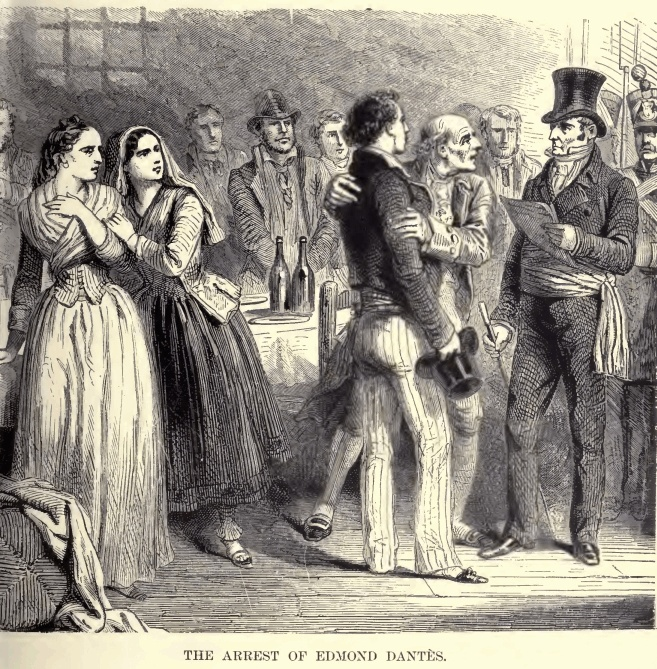
\includegraphics[width=\textwidth]{0075m.jpg}
\end{figure}

“Oh, to be sure!” responded Danglars, who had now approached the group,
“nothing more than a mistake, I feel quite certain.”

Dantès descended the staircase, preceded by the magistrate, and
followed by the soldiers. A carriage awaited him at the door; he got
in, followed by two soldiers and the magistrate, and the vehicle drove
off towards Marseilles.

“Adieu, adieu, dearest Edmond!” cried Mercédès, stretching out her arms
to him from the balcony.

The prisoner heard the cry, which sounded like the sob of a broken
heart, and leaning from the coach he called out, “Good-bye, Mercédès—we
shall soon meet again!” Then the vehicle disappeared round one of the
turnings of Fort Saint Nicholas.

“Wait for me here, all of you!” cried M. Morrel; “I will take the first
conveyance I find, and hurry to Marseilles, whence I will bring you
word how all is going on.”

“That’s right!” exclaimed a multitude of voices, “go, and return as
quickly as you can!”

This second departure was followed by a long and fearful state of
terrified silence on the part of those who were left behind. The old
father and Mercédès remained for some time apart, each absorbed in
grief; but at length the two poor victims of the same blow raised their
eyes, and with a simultaneous burst of feeling rushed into each other’s
arms.

Meanwhile Fernand made his appearance, poured out for himself a glass
of water with a trembling hand; then hastily swallowing it, went to sit
down at the first vacant place, and this was, by mere chance, placed
next to the seat on which poor Mercédès had fallen half fainting, when
released from the warm and affectionate embrace of old Dantès.
Instinctively Fernand drew back his chair.

“He is the cause of all this misery—I am quite sure of it,” whispered
Caderousse, who had never taken his eyes off Fernand, to Danglars.

“I don’t think so,” answered the other; “he’s too stupid to imagine
such a scheme. I only hope the mischief will fall upon the head of
whoever wrought it.”

“You don’t mention those who aided and abetted the deed,” said
Caderousse.

“Surely,” answered Danglars, “one cannot be held responsible for every
chance arrow shot into the air.”

“You can, indeed, when the arrow lights point downward on somebody’s
head.”

Meantime the subject of the arrest was being canvassed in every
different form.

“What think you, Danglars,” said one of the party, turning towards him,
“of this event?”

“Why,” replied he, “I think it just possible Dantès may have been
detected with some trifling article on board ship considered here as
contraband.”

“But how could he have done so without your knowledge, Danglars, since
you are the ship’s supercargo?”

“Why, as for that, I could only know what I was told respecting the
merchandise with which the vessel was laden. I know she was loaded with
cotton, and that she took in her freight at Alexandria from Pastret’s
warehouse, and at Smyrna from Pascal’s; that is all I was obliged to
know, and I beg I may not be asked for any further particulars.”

“Now I recollect,” said the afflicted old father; “my poor boy told me
yesterday he had got a small case of coffee, and another of tobacco for
me!”

“There, you see,” exclaimed Danglars. “Now the mischief is out; depend
upon it the custom-house people went rummaging about the ship in our
absence, and discovered poor Dantès’ hidden treasures.”

Mercédès, however, paid no heed to this explanation of her lover’s
arrest. Her grief, which she had hitherto tried to restrain, now burst
out in a violent fit of hysterical sobbing.

“Come, come,” said the old man, “be comforted, my poor child; there is
still hope!”

“Hope!” repeated Danglars.

“Hope!” faintly murmured Fernand, but the word seemed to die away on
his pale agitated lips, and a convulsive spasm passed over his
countenance.

“Good news! good news!” shouted forth one of the party stationed in the
balcony on the lookout. “Here comes M. Morrel back. No doubt, now, we
shall hear that our friend is released!”

Mercédès and the old man rushed to meet the shipowner and greeted him
at the door. He was very pale.

“What news?” exclaimed a general burst of voices.

“Alas, my friends,” replied M. Morrel, with a mournful shake of his
head, “the thing has assumed a more serious aspect than I expected.”

“Oh, indeed—indeed, sir, he is innocent!” sobbed forth Mercédès.

“That I believe!” answered M. Morrel; “but still he is charged——”

“With what?” inquired the elder Dantès.

“With being an agent of the Bonapartist faction!” Many of our readers
may be able to recollect how formidable such an accusation became in
the period at which our story is dated.

A despairing cry escaped the pale lips of Mercédès; the old man sank
into a chair.

“Ah, Danglars!” whispered Caderousse, “you have deceived me—the trick
you spoke of last night has been played; but I cannot suffer a poor old
man or an innocent girl to die of grief through your fault. I am
determined to tell them all about it.”

“Be silent, you simpleton!” cried Danglars, grasping him by the arm,
“or I will not answer even for your own safety. Who can tell whether
Dantès be innocent or guilty? The vessel did touch at Elba, where he
quitted it, and passed a whole day in the island. Now, should any
letters or other documents of a compromising character be found upon
him, will it not be taken for granted that all who uphold him are his
accomplices?”

With the rapid instinct of selfishness, Caderousse readily perceived
the solidity of this mode of reasoning; he gazed, doubtfully,
wistfully, on Danglars, and then caution supplanted generosity.

“Suppose we wait a while, and see what comes of it,” said he, casting a
bewildered look on his companion.

“To be sure!” answered Danglars. “Let us wait, by all means. If he be
innocent, of course he will be set at liberty; if guilty, why, it is no
use involving ourselves in a conspiracy.”

“Let us go, then. I cannot stay here any longer.”

“With all my heart!” replied Danglars, pleased to find the other so
tractable. “Let us take ourselves out of the way, and leave things for
the present to take their course.”

After their departure, Fernand, who had now again become the friend and
protector of Mercédès, led the girl to her home, while some friends of
Dantès conducted his father, nearly lifeless, to the Allées de Meilhan.

The rumor of Edmond’s arrest as a Bonapartist agent was not slow in
circulating throughout the city.

“Could you ever have credited such a thing, my dear Danglars?” asked M.
Morrel, as, on his return to the port for the purpose of gleaning fresh
tidings of Dantès, from M. de Villefort, the assistant procureur, he
overtook his supercargo and Caderousse. “Could you have believed such a
thing possible?”

“Why, you know I told you,” replied Danglars, “that I considered the
circumstance of his having anchored at the Island of Elba as a very
suspicious circumstance.”

“And did you mention these suspicions to any person beside myself?”

\begin{figure}[ht]
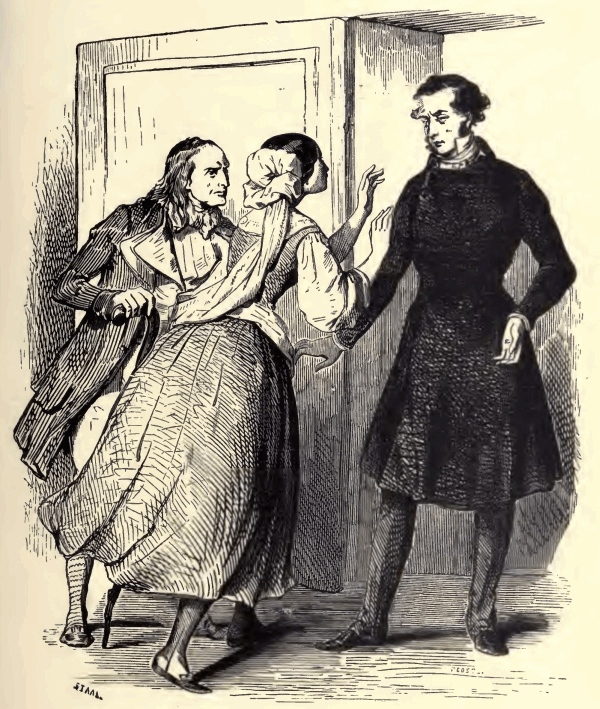
\includegraphics[width=\textwidth]{0079m.jpg}
\end{figure}

“Certainly not!” returned Danglars. Then added in a low whisper, “You
understand that, on account of your uncle, M. Policar Morrel, who
served under the \textit{other} government, and who does not altogether
conceal what he thinks on the subject, you are strongly suspected of
regretting the abdication of Napoleon. I should have feared to injure
both Edmond and yourself, had I divulged my own apprehensions to a
soul. I am too well aware that though a subordinate, like myself, is
bound to acquaint the shipowner with everything that occurs, there are
many things he ought most carefully to conceal from all else.”

“’Tis well, Danglars—’tis well!” replied M. Morrel. “You are a worthy
fellow; and I had already thought of your interests in the event of
poor Edmond having become captain of the \textit{Pharaon}.”

“Is it possible you were so kind?”

“Yes, indeed; I had previously inquired of Dantès what was his opinion
of you, and if he should have any reluctance to continue you in your
post, for somehow I have perceived a sort of coolness between you.”

“And what was his reply?”

“That he certainly did think he had given you offence in an affair
which he merely referred to without entering into particulars, but that
whoever possessed the good opinion and confidence of the ship’s owners
would have his preference also.”

“The hypocrite!” murmured Danglars.

“Poor Dantès!” said Caderousse. “No one can deny his being a
noble-hearted young fellow.”

“But meanwhile,” continued M. Morrel, “here is the \textit{Pharaon} without a
captain.”

“Oh,” replied Danglars, “since we cannot leave this port for the next
three months, let us hope that ere the expiration of that period Dantès
will be set at liberty.”

“No doubt; but in the meantime?”

“I am entirely at your service, M. Morrel,” answered Danglars. “You
know that I am as capable of managing a ship as the most experienced
captain in the service; and it will be so far advantageous to you to
accept my services, that upon Edmond’s release from prison no further
change will be requisite on board the \textit{Pharaon} than for Dantès and
myself each to resume our respective posts.”

“Thanks, Danglars—that will smooth over all difficulties. I fully
authorize you at once to assume the command of the \textit{Pharaon}, and look
carefully to the unloading of her freight. Private misfortunes must
never be allowed to interfere with business.”

“Be easy on that score, M. Morrel; but do you think we shall be
permitted to see our poor Edmond?”

“I will let you know that directly I have seen M. de Villefort, whom I
shall endeavor to interest in Edmond’s favor. I am aware he is a
furious royalist; but, in spite of that, and of his being king’s
attorney, he is a man like ourselves, and I fancy not a bad sort of
one.”

“Perhaps not,” replied Danglars; “but I hear that he is ambitious, and
that’s rather against him.”

“Well, well,” returned M. Morrel, “we shall see. But now hasten on
board, I will join you there ere long.”

So saying, the worthy shipowner quitted the two allies, and proceeded
in the direction of the Palais de Justice.

\begin{figure}[h]
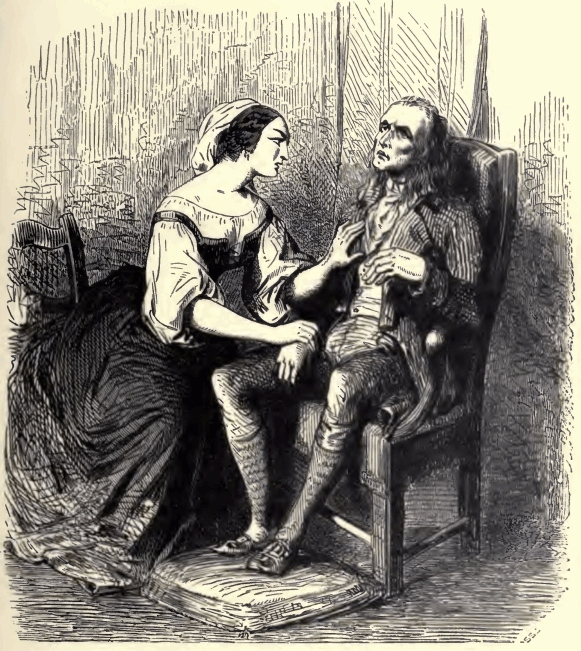
\includegraphics[width=\textwidth]{0081m.jpg}
\end{figure}

“You see,” said Danglars, addressing Caderousse, “the turn things have
taken. Do you still feel any desire to stand up in his defence?”

“Not the slightest, but yet it seems to me a shocking thing that a mere
joke should lead to such consequences.”

“But who perpetrated that joke, let me ask? neither you nor myself, but
Fernand; you knew very well that I threw the paper into a corner of the
room—indeed, I fancied I had destroyed it.”

“Oh, no,” replied Caderousse, “that I can answer for, you did not. I
only wish I could see it now as plainly as I saw it lying all crushed
and crumpled in a corner of the arbor.”

“Well, then, if you did, depend upon it, Fernand picked it up, and
either copied it or caused it to be copied; perhaps, even, he did not
take the trouble of recopying it. And now I think of it, by Heavens, he
may have sent the letter itself! Fortunately, for me, the handwriting
was disguised.”

“Then you were aware of Dantès being engaged in a conspiracy?”

“Not I. As I before said, I thought the whole thing was a joke, nothing
more. It seems, however, that I have unconsciously stumbled upon the
truth.”

“Still,” argued Caderousse, “I would give a great deal if nothing of
the kind had happened; or, at least, that I had had no hand in it. You
will see, Danglars, that it will turn out an unlucky job for both of
us.”

“Nonsense! If any harm come of it, it should fall on the guilty person;
and that, you know, is Fernand. How can we be implicated in any way?
All we have got to do is, to keep our own counsel, and remain perfectly
quiet, not breathing a word to any living soul; and you will see that
the storm will pass away without in the least affecting us.”

“Amen!” responded Caderousse, waving his hand in token of adieu to
Danglars, and bending his steps towards the Allées de Meilhan, moving
his head to and fro, and muttering as he went, after the manner of one
whose mind was overcharged with one absorbing idea.

“So far, then,” said Danglars, mentally, “all has gone as I would have
it. I am, temporarily, commander of the \textit{Pharaon}, with the certainty
of being permanently so, if that fool of a Caderousse can be persuaded
to hold his tongue. My only fear is the chance of Dantès being
released. But, there, he is in the hands of Justice; and,” added he
with a smile, “she will take her own.” So saying, he leaped into a
boat, desiring to be rowed on board the \textit{Pharaon}, where M. Morrel had
agreed to meet him.

\printpagenotes*
\chapter{The Deputy Procureur du Roi}

In one of the aristocratic mansions built by Puget in the Rue du Grand
Cours opposite the Medusa fountain, a second marriage feast was being
celebrated, almost at the same hour with the nuptial repast given by
Dantès. In this case, however, although the occasion of the
entertainment was similar, the company was strikingly dissimilar.
Instead of a rude mixture of sailors, soldiers, and those belonging to
the humblest grade of life, the present assembly was composed of the
very flower of Marseilles society,—magistrates who had resigned their
office during the usurper’s reign; officers who had deserted from the
imperial army and joined forces with Condé; and younger members of
families, brought up to hate and execrate the man whom five years of
exile would convert into a martyr, and fifteen of restoration elevate
to the rank of a god.

The guests were still at table, and the heated and energetic
conversation that prevailed betrayed the violent and vindictive
passions that then agitated each dweller of the South, where unhappily,
for five centuries religious strife had long given increased bitterness
to the violence of party feeling.

The emperor, now king of the petty Island of Elba, after having held
sovereign sway over one-half of the world, counting as his subjects a
small population of five or six thousand souls,—after having been
accustomed to hear the “\textit{Vive Napoléons}” of a hundred and twenty
millions of human beings, uttered in ten different languages,—was
looked upon here as a ruined man, separated forever from any fresh
connection with France or claim to her throne.

The magistrates freely discussed their political views; the military
part of the company talked unreservedly of Moscow and Leipsic, while
the women commented on the divorce of Josephine. It was not over the
downfall of the man, but over the defeat of the Napoleonic idea, that
they rejoiced, and in this they foresaw for themselves the bright and
cheering prospect of a revivified political existence.

An old man, decorated with the cross of Saint Louis, now rose and
proposed the health of King Louis XVIII. It was the Marquis de
Saint-Méran. This toast, recalling at once the patient exile of
Hartwell and the peace-loving King of France, excited universal
enthusiasm; glasses were elevated in the air \textit{à l’Anglaise}, and the
ladies, snatching their bouquets from their fair bosoms, strewed the
table with their floral treasures. In a word, an almost poetical fervor
prevailed.

“Ah,” said the Marquise de Saint-Méran, a woman with a stern,
forbidding eye, though still noble and distinguished in appearance,
despite her fifty years—“ah, these revolutionists, who have driven us
from those very possessions they afterwards purchased for a mere trifle
during the Reign of Terror, would be compelled to own, were they here,
that all true devotion was on our side, since we were content to follow
the fortunes of a falling monarch, while they, on the contrary, made
their fortune by worshipping the rising sun; yes, yes, they could not
help admitting that the king, for whom we sacrificed rank, wealth, and
station was truly our ‘Louis the well-beloved,’ while their wretched
usurper has been, and ever will be, to them their evil genius, their
‘Napoleon the accursed.’ Am I not right, Villefort?”

“I beg your pardon, madame. I really must pray you to excuse me, but—in
truth—I was not attending to the conversation.”

“Marquise, marquise!” interposed the old nobleman who had proposed the
toast, “let the young people alone; let me tell you, on one’s wedding
day there are more agreeable subjects of conversation than dry
politics.”

“Never mind, dearest mother,” said a young and lovely girl, with a
profusion of light brown hair, and eyes that seemed to float in liquid
crystal, “’tis all my fault for seizing upon M. de Villefort, so as to
prevent his listening to what you said. But there—now take him—he is
your own for as long as you like. M. Villefort, I beg to remind you my
mother speaks to you.”

“If the marquise will deign to repeat the words I but imperfectly
caught, I shall be delighted to answer,” said M. de Villefort.

“Never mind, Renée,” replied the marquise, with a look of tenderness
that seemed out of keeping with her harsh dry features; but, however
all other feelings may be withered in a woman’s nature, there is always
one bright smiling spot in the desert of her heart, and that is the
shrine of maternal love. “I forgive you. What I was saying, Villefort,
was, that the Bonapartists had not our sincerity, enthusiasm, or
devotion.”

“They had, however, what supplied the place of those fine qualities,”
replied the young man, “and that was fanaticism. Napoleon is the
Mahomet of the West, and is worshipped by his commonplace but ambitious
followers, not only as a leader and lawgiver, but also as the
personification of equality.”

“He!” cried the marquise: “Napoleon the type of equality! For mercy’s
sake, then, what would you call Robespierre? Come, come, do not strip
the latter of his just rights to bestow them on the Corsican, who, to
my mind, has usurped quite enough.”

\begin{figure}[h]
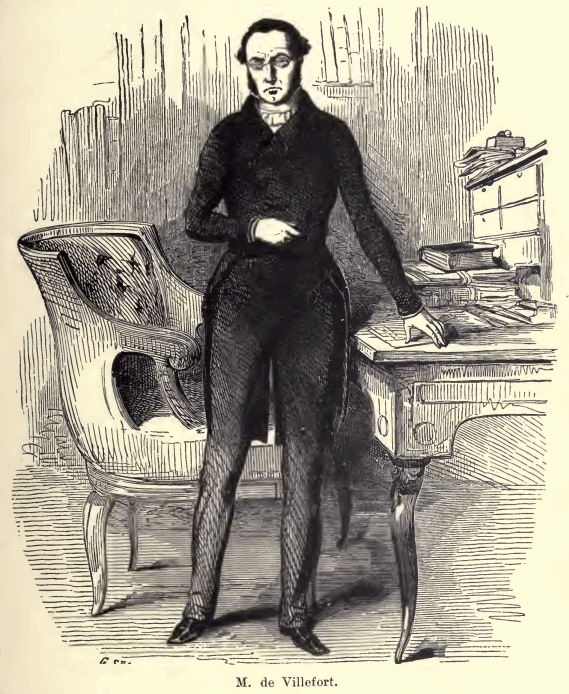
\includegraphics[width=\textwidth]{0085m.jpg}
\end{figure}

“Nay, madame; I would place each of these heroes on his right
pedestal—that of Robespierre on his scaffold in the Place Louis Quinze;
that of Napoleon on the column of the Place Vendôme. The only
difference consists in the opposite character of the equality advocated
by these two men; one is the equality that elevates, the other is the
equality that degrades; one brings a king within reach of the
guillotine, the other elevates the people to a level with the throne.
Observe,” said Villefort, smiling, “I do not mean to deny that both
these men were revolutionary scoundrels, and that the 9th Thermidor and
the 4th of April, in the year 1814, were lucky days for France, worthy
of being gratefully remembered by every friend to monarchy and civil
order; and that explains how it comes to pass that, fallen, as I trust
he is forever, Napoleon has still retained a train of parasitical
satellites. Still, marquise, it has been so with other
usurpers—Cromwell, for instance, who was not half so bad as Napoleon,
had his partisans and advocates.”

“Do you know, Villefort, that you are talking in a most dreadfully
revolutionary strain? But I excuse it, it is impossible to expect the
son of a Girondin to be free from a small spice of the old leaven.” A
deep crimson suffused the countenance of Villefort.

“’Tis true, madame,” answered he, “that my father was a Girondin, but
he was not among the number of those who voted for the king’s death; he
was an equal sufferer with yourself during the Reign of Terror, and had
well-nigh lost his head on the same scaffold on which your father
perished.”

“True,” replied the marquise, without wincing in the slightest degree
at the tragic remembrance thus called up; “but bear in mind, if you
please, that our respective parents underwent persecution and
proscription from diametrically opposite principles; in proof of which
I may remark, that while my family remained among the staunchest
adherents of the exiled princes, your father lost no time in joining
the new government; and that while the Citizen Noirtier was a Girondin,
the Count Noirtier became a senator.”

“Dear mother,” interposed Renée, “you know very well it was agreed that
all these disagreeable reminiscences should forever be laid aside.”

“Suffer me, also, madame,” replied Villefort, “to add my earnest
request to Mademoiselle de Saint-Méran’s, that you will kindly allow
the veil of oblivion to cover and conceal the past. What avails
recrimination over matters wholly past recall? For my own part, I have
laid aside even the name of my father, and altogether disown his
political principles. He was—nay, probably may still be—a Bonapartist,
and is called Noirtier; I, on the contrary, am a staunch royalist, and
style myself de Villefort. Let what may remain of revolutionary sap
exhaust itself and die away with the old trunk, and condescend only to
regard the young shoot which has started up at a distance from the
parent tree, without having the power, any more than the wish, to
separate entirely from the stock from which it sprung.”

“Bravo, Villefort!” cried the marquis; “excellently well said! Come,
now, I have hopes of obtaining what I have been for years endeavoring
to persuade the marquise to promise; namely, a perfect amnesty and
forgetfulness of the past.”

“With all my heart,” replied the marquise; “let the past be forever
forgotten. I promise you it affords \textit{me} as little pleasure to revive
it as it does you. All I ask is, that Villefort will be firm and
inflexible for the future in his political principles. Remember, also,
Villefort, that we have pledged ourselves to his majesty for your
fealty and strict loyalty, and that at our recommendation the king
consented to forget the past, as I do” (and here she extended to him
her hand)—“as I now do at your entreaty. But bear in mind, that should
there fall in your way anyone guilty of conspiring against the
government, you will be so much the more bound to visit the offence
with rigorous punishment, as it is known you belong to a suspected
family.”

“Alas, madame,” returned Villefort, “my profession, as well as the
times in which we live, compels me to be severe. I have already
successfully conducted several public prosecutions, and brought the
offenders to merited punishment. But we have not done with the thing
yet.”

\begin{figure}[h]
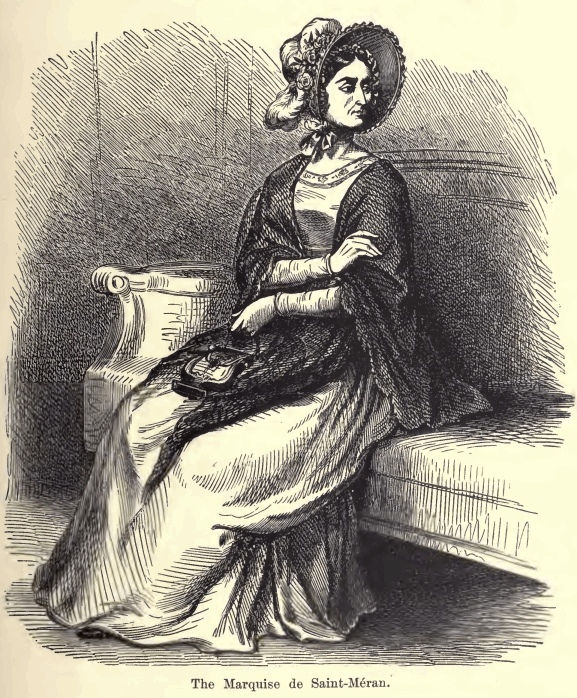
\includegraphics[width=\textwidth]{0087m.jpg}
\end{figure}

“Do you, indeed, think so?” inquired the marquise.

“I am, at least, fearful of it. Napoleon, in the Island of Elba, is too
near France, and his proximity keeps up the hopes of his partisans.
Marseilles is filled with half-pay officers, who are daily, under one
frivolous pretext or other, getting up quarrels with the royalists;
from hence arise continual and fatal duels among the higher classes of
persons, and assassinations in the lower.”

“You have heard, perhaps,” said the Comte de Salvieux, one of M. de
Saint-Méran’s oldest friends, and chamberlain to the Comte d’Artois,
“that the Holy Alliance purpose removing him from thence?”

“Yes; they were talking about it when we left Paris,” said M. de
Saint-Méran; “and where is it decided to transfer him?”

“To Saint Helena.”

“For heaven’s sake, where is that?” asked the marquise.

“An island situated on the other side of the equator, at least two
thousand leagues from here,” replied the count.

“So much the better. As Villefort observes, it is a great act of folly
to have left such a man between Corsica, where he was born, and Naples,
of which his brother-in-law is king, and face to face with Italy, the
sovereignty of which he coveted for his son.”

“Unfortunately,” said Villefort, “there are the treaties of 1814, and
we cannot molest Napoleon without breaking those compacts.”

“Oh, well, we shall find some way out of it,” responded M. de Salvieux.
“There wasn’t any trouble over treaties when it was a question of
shooting the poor Duc d’Enghien.”

“Well,” said the marquise, “it seems probable that, by the aid of the
Holy Alliance, we shall be rid of Napoleon; and we must trust to the
vigilance of M. de Villefort to purify Marseilles of his partisans. The
king is either a king or no king; if he be acknowledged as sovereign of
France, he should be upheld in peace and tranquillity; and this can
best be effected by employing the most inflexible agents to put down
every attempt at conspiracy—’tis the best and surest means of
preventing mischief.”

“Unfortunately, madame,” answered Villefort, “the strong arm of the law
is not called upon to interfere until the evil has taken place.”

“Then all he has got to do is to endeavor to repair it.”

“Nay, madame, the law is frequently powerless to effect this; all it
can do is to avenge the wrong done.”

“Oh, M. de Villefort,” cried a beautiful young creature, daughter to
the Comte de Salvieux, and the cherished friend of Mademoiselle de
Saint-Méran, “do try and get up some famous trial while we are at
Marseilles. I never was in a law-court; I am told it is so very
amusing!”

“Amusing, certainly,” replied the young man, “inasmuch as, instead of
shedding tears as at the fictitious tale of woe produced at a theatre,
you behold in a law-court a case of real and genuine distress—a drama
of life. The prisoner whom you there see pale, agitated, and alarmed,
instead of—as is the case when a curtain falls on a tragedy—going home
to sup peacefully with his family, and then retiring to rest, that he
may recommence his mimic woes on the morrow,—is removed from your sight
merely to be reconducted to his prison and delivered up to the
executioner. I leave you to judge how far your nerves are calculated to
bear you through such a scene. Of this, however, be assured, that
should any favorable opportunity present itself, I will not fail to
offer you the choice of being present.”

“For shame, M. de Villefort!” said Renée, becoming quite pale; “don’t
you see how you are frightening us?—and yet you laugh.”

“What would you have? ’Tis like a duel. I have already recorded
sentence of death, five or six times, against the movers of political
conspiracies, and who can say how many daggers may be ready sharpened,
and only waiting a favorable opportunity to be buried in my heart?”

“Gracious heavens, M. de Villefort,” said Renée, becoming more and more
terrified; “you surely are not in earnest.”

“Indeed I am,” replied the young magistrate with a smile; “and in the
interesting trial that young lady is anxious to witness, the case would
only be still more aggravated. Suppose, for instance, the prisoner, as
is more than probable, to have served under Napoleon—well, can you
expect for an instant, that one accustomed, at the word of his
commander, to rush fearlessly on the very bayonets of his foe, will
scruple more to drive a stiletto into the heart of one he knows to be
his personal enemy, than to slaughter his fellow-creatures, merely
because bidden to do so by one he is bound to obey? Besides, one
requires the excitement of being hateful in the eyes of the accused, in
order to lash one’s self into a state of sufficient vehemence and
power. I would not choose to see the man against whom I pleaded smile,
as though in mockery of my words. No; my pride is to see the accused
pale, agitated, and as though beaten out of all composure by the fire
of my eloquence.” Renée uttered a smothered exclamation.

“Bravo!” cried one of the guests; “that is what I call talking to some
purpose.”

“Just the person we require at a time like the present,” said a second.

“What a splendid business that last case of yours was, my dear
Villefort!” remarked a third; “I mean the trial of the man for
murdering his father. Upon my word, you killed him ere the executioner
had laid his hand upon him.”

“Oh, as for parricides, and such dreadful people as that,” interposed
Renée, “it matters very little what is done to them; but as regards
poor unfortunate creatures whose only crime consists in having mixed
themselves up in political intrigues——”

“Why, that is the very worst offence they could possibly commit; for,
don’t you see, Renée, the king is the father of his people, and he who
shall plot or contrive aught against the life and safety of the parent
of thirty-two millions of souls, is a parricide upon a fearfully great
scale?”

“I don’t know anything about that,” replied Renée; “but, M. de
Villefort, you have promised me—have you not?—always to show mercy to
those I plead for.”

“Make yourself quite easy on that point,” answered Villefort, with one
of his sweetest smiles; “you and I will always consult upon our
verdicts.”

“My love,” said the marquise, “attend to your doves, your lap-dogs, and
embroidery, but do not meddle with what you do not understand. Nowadays
the military profession is in abeyance and the magisterial robe is the
badge of honor. There is a wise Latin proverb that is very much in
point.”

“\textit{Cedant arma togæ},” said Villefort with a bow.

“I cannot speak Latin,” responded the marquise.

“Well,” said Renée, “I cannot help regretting you had not chosen some
other profession than your own—a physician, for instance. Do you know I
always felt a shudder at the idea of even a \textit{destroying} angel?”

“Dear, good Renée,” whispered Villefort, as he gazed with unutterable
tenderness on the lovely speaker.

“Let us hope, my child,” cried the marquis, “that M. de Villefort may
prove the moral and political physician of this province; if so, he
will have achieved a noble work.”

“And one which will go far to efface the recollection of his father’s
conduct,” added the incorrigible marquise.

“Madame,” replied Villefort, with a mournful smile, “I have already had
the honor to observe that my father has—at least, I hope so—abjured his
past errors, and that he is, at the present moment, a firm and zealous
friend to religion and order—a better royalist, possibly, than his son;
for he has to atone for past dereliction, while I have no other impulse
than warm, decided preference and conviction.” Having made this
well-turned speech, Villefort looked carefully around to mark the
effect of his oratory, much as he would have done had he been
addressing the bench in open court.

“Do you know, my dear Villefort,” cried the Comte de Salvieux, “that is
exactly what I myself said the other day at the Tuileries, when
questioned by his majesty’s principal chamberlain touching the
singularity of an alliance between the son of a Girondin and the
daughter of an officer of the Duc de Condé; and I assure you he seemed
fully to comprehend that this mode of reconciling political differences
was based upon sound and excellent principles. Then the king, who,
without our suspecting it, had overheard our conversation, interrupted
us by saying, ‘Villefort’—observe that the king did not pronounce the
word Noirtier, but, on the contrary, placed considerable emphasis on
that of Villefort—‘Villefort,’ said his majesty, ‘is a young man of
great judgment and discretion, who will be sure to make a figure in his
profession; I like him much, and it gave me great pleasure to hear that
he was about to become the son-in-law of the Marquis and Marquise de
Saint-Méran. I should myself have recommended the match, had not the
noble marquis anticipated my wishes by requesting my consent to it.’”

“Is it possible the king could have condescended so far as to express
himself so favorably of me?” asked the enraptured Villefort.

“I give you his very words; and if the marquis chooses to be candid, he
will confess that they perfectly agree with what his majesty said to
him, when he went six months ago to consult him upon the subject of
your espousing his daughter.”

\begin{figure}[h]
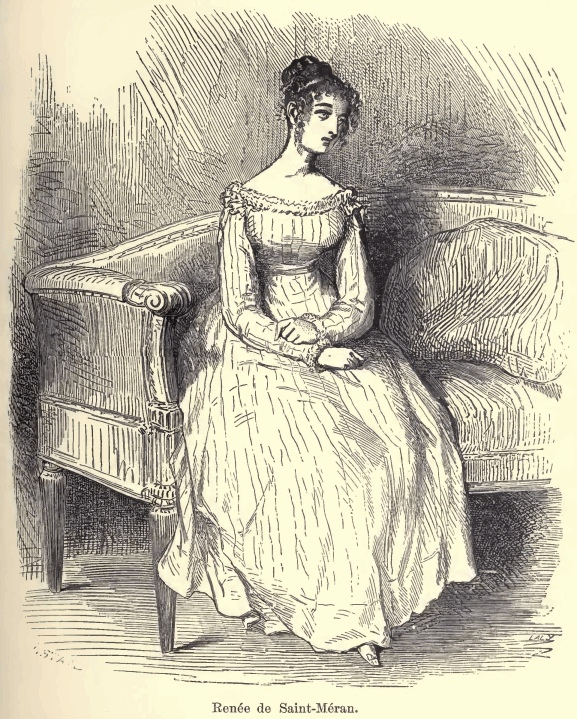
\includegraphics[width=\textwidth]{0091m.jpg}
\end{figure}

“That is true,” answered the marquis.

“How much do I owe this gracious prince! What is there I would not do
to evince my earnest gratitude!”

“That is right,” cried the marquise. “I love to see you thus. Now,
then, were a conspirator to fall into your hands, he would be most
welcome.”

“For my part, dear mother,” interposed Renée, “I trust your wishes will
not prosper, and that Providence will only permit petty offenders, poor
debtors, and miserable cheats to fall into M. de Villefort’s
hands,—then I shall be contented.”

“Just the same as though you prayed that a physician might only be
called upon to prescribe for headaches, measles, and the stings of
wasps, or any other slight affection of the epidermis. If you wish to
see me the king’s attorney, you must desire for me some of those
violent and dangerous diseases from the cure of which so much honor
redounds to the physician.”

At this moment, and as though the utterance of Villefort’s wish had
sufficed to effect its accomplishment, a servant entered the room, and
whispered a few words in his ear. Villefort immediately rose from table
and quitted the room upon the plea of urgent business; he soon,
however, returned, his whole face beaming with delight. Renée regarded
him with fond affection; and certainly his handsome features, lit up as
they then were with more than usual fire and animation, seemed formed
to excite the innocent admiration with which she gazed on her graceful
and intelligent lover.

“You were wishing just now,” said Villefort, addressing her, “that I
were a doctor instead of a lawyer. Well, I at least resemble the
disciples of Esculapius in one thing [people spoke in this style in
1815], that of not being able to call a day my own, not even that of my
betrothal.”

“And wherefore were you called away just now?” asked Mademoiselle de
Saint-Méran, with an air of deep interest.

“For a very serious matter, which bids fair to make work for the
executioner.”

“How dreadful!” exclaimed Renée, turning pale.

“Is it possible?” burst simultaneously from all who were near enough to
the magistrate to hear his words.

“Why, if my information prove correct, a sort of Bonapartist conspiracy
has just been discovered.”

“Can I believe my ears?” cried the marquise.

“I will read you the letter containing the accusation, at least,” said
Villefort:

“‘The king’s attorney is informed by a friend to the throne and the
religious institutions of his country, that one named Edmond Dantès,
mate of the ship \textit{Pharaon}, this day arrived from Smyrna, after having
touched at Naples and Porto-Ferrajo, has been the bearer of a letter
from Murat to the usurper, and again taken charge of another letter
from the usurper to the Bonapartist club in Paris. Ample corroboration
of this statement may be obtained by arresting the above-mentioned
Edmond Dantès, who either carries the letter for Paris about with him,
or has it at his father’s abode. Should it not be found in the
possession of father or son, then it will assuredly be discovered in
the cabin belonging to the said Dantès on board the \textit{Pharaon}.’”

“But,” said Renée, “this letter, which, after all, is but an anonymous
scrawl, is not even addressed to you, but to the king’s attorney.”

\begin{figure}[h]
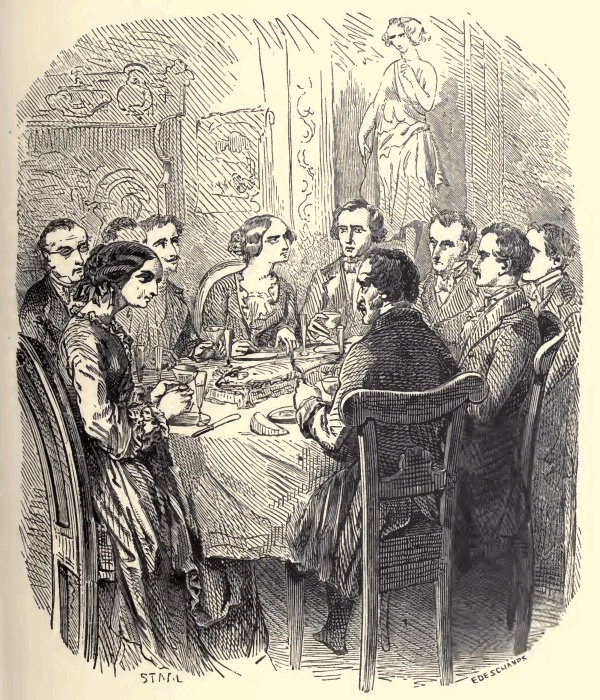
\includegraphics[width=\textwidth]{0093m.jpg}
\end{figure}

“True; but that gentleman being absent, his secretary, by his orders,
opened his letters; thinking this one of importance, he sent for me,
but not finding me, took upon himself to give the necessary orders for
arresting the accused party.”

“Then the guilty person is absolutely in custody?” said the marquise.

“Nay, dear mother, say the accused person. You know we cannot yet
pronounce him guilty.”

“He is in safe custody,” answered Villefort; “and rely upon it, if the
letter is found, he will not be likely to be trusted abroad again,
unless he goes forth under the especial protection of the headsman.”

“And where is the unfortunate being?” asked Renée.

“He is at my house.”

“Come, come, my friend,” interrupted the marquise, “do not neglect your
duty to linger with us. You are the king’s servant, and must go
wherever that service calls you.”

“Oh, Villefort!” cried Renée, clasping her hands, and looking towards
her lover with piteous earnestness, “be merciful on this the day of our
betrothal.”

The young man passed round to the side of the table where the fair
pleader sat, and leaning over her chair said tenderly:

“To give you pleasure, my sweet Renée, I promise to show all the lenity
in my power; but if the charges brought against this Bonapartist hero
prove correct, why, then, you really must give me leave to order his
head to be cut off.”

Renée shuddered at the word \textit{cut}, for the growth in question had a
head.

“Never mind that foolish girl, Villefort,” said the marquise. “She will
soon get over these things.” So saying, Madame de Saint-Méran extended
her dry bony hand to Villefort, who, while imprinting a son-in-law’s
respectful salute on it, looked at Renée, as much as to say, “I must
try and fancy ’tis your dear hand I kiss, as it should have been.”

“These are mournful auspices to accompany a betrothal,” sighed poor
Renée.

“Upon my word, child!” exclaimed the angry marquise, “your folly
exceeds all bounds. I should be glad to know what connection there can
possibly be between your sickly sentimentality and the affairs of the
state!”

“Oh, mother!” murmured Renée.

“Nay, madame, I pray you pardon this little traitor. I promise you that
to make up for her want of loyalty, I will be most inflexibly severe;”
then casting an expressive glance at his betrothed, which seemed to
say, “Fear not, for your dear sake my justice shall be tempered with
mercy,” and receiving a sweet and approving smile in return, Villefort
departed with paradise in his heart.

\printpagenotes*
\chapter{The Examination}

No sooner had Villefort left the salon, than he assumed the grave air
of a man who holds the balance of life and death in his hands. Now, in
spite of the nobility of his countenance, the command of which, like a
finished actor, he had carefully studied before the glass, it was by no
means easy for him to assume an air of judicial severity. Except the
recollection of the line of politics his father had adopted, and which
might interfere, unless he acted with the greatest prudence, with his
own career, Gérard de Villefort was as happy as a man could be. Already
rich, he held a high official situation, though only twenty-seven. He
was about to marry a young and charming woman, whom he loved, not
passionately, but reasonably, as became a deputy attorney of the king;
and besides her personal attractions, which were very great,
Mademoiselle de Saint-Méran’s family possessed considerable political
influence, which they would, of course, exert in his favor. The dowry
of his wife amounted to fifty thousand crowns, and he had, besides, the
prospect of seeing her fortune increased to half a million at her
father’s death. These considerations naturally gave Villefort a feeling
of such complete felicity that his mind was fairly dazzled in its
contemplation.

At the door he met the commissary of police, who was waiting for him.
The sight of this officer recalled Villefort from the third heaven to
earth; he composed his face, as we have before described, and said, “I
have read the letter, sir, and you have acted rightly in arresting this
man; now inform me what you have discovered concerning him and the
conspiracy.”

“We know nothing as yet of the conspiracy, monsieur; all the papers
found have been sealed up and placed on your desk. The prisoner himself
is named Edmond Dantès, mate on board the three-master the \textit{Pharaon},
trading in cotton with Alexandria and Smyrna, and belonging to Morrel \&
Son, of Marseilles.”

“Before he entered the merchant service, had he ever served in the
marines?”

“Oh, no, monsieur, he is very young.”

“How old?”

“Nineteen or twenty at the most.”

At this moment, and as Villefort had arrived at the corner of the Rue
des Conseils, a man, who seemed to have been waiting for him,
approached; it was M. Morrel.

“Ah, M. de Villefort,” cried he, “I am delighted to see you. Some of
your people have committed the strangest mistake—they have just
arrested Edmond Dantès, mate of my vessel.”

“I know it, monsieur,” replied Villefort, “and I am now going to
examine him.”

“Oh,” said Morrel, carried away by his friendship, “you do not know
him, and I do. He is the most estimable, the most trustworthy creature
in the world, and I will venture to say, there is not a better seaman
in all the merchant service. Oh, M. de Villefort, I beseech your
indulgence for him.”

Villefort, as we have seen, belonged to the aristocratic party at
Marseilles, Morrel to the plebeian; the first was a royalist, the other
suspected of Bonapartism. Villefort looked disdainfully at Morrel, and
replied coldly:

“You are aware, monsieur, that a man may be estimable and trustworthy
in private life, and the best seaman in the merchant service, and yet
be, politically speaking, a great criminal. Is it not true?”

The magistrate laid emphasis on these words, as if he wished to apply
them to the owner himself, while his eyes seemed to plunge into the
heart of one who, interceding for another, had himself need of
indulgence. Morrel reddened, for his own conscience was not quite clear
on politics; besides, what Dantès had told him of his interview with
the grand-marshal, and what the emperor had said to him, embarrassed
him. He replied, however, in a tone of deep interest:

“I entreat you, M. de Villefort, be, as you always are, kind and
equitable, and give him back to us soon.” This \textit{give us} sounded
revolutionary in the deputy’s ears.

“Ah, ah,” murmured he, “is Dantès then a member of some Carbonari
society, that his protector thus employs the collective form? He was,
if I recollect, arrested in a tavern, in company with a great many
others.” Then he added, “Monsieur, you may rest assured I shall perform
my duty impartially, and that if he be innocent you shall not have
appealed to me in vain; should he, however, be guilty, in this present
epoch, impunity would furnish a dangerous example, and I must do my
duty.”

\begin{figure}[ht]
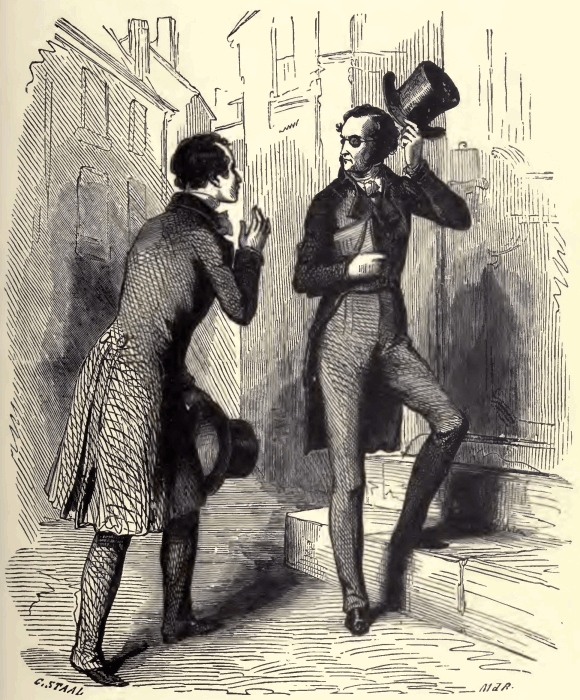
\includegraphics[width=\textwidth]{0097m.jpg}
\end{figure}

As he had now arrived at the door of his own house, which adjoined the
Palais de Justice, he entered, after having, coldly saluted the
shipowner, who stood, as if petrified, on the spot where Villefort had
left him. The antechamber was full of police agents and gendarmes, in
the midst of whom, carefully watched, but calm and smiling, stood the
prisoner. Villefort traversed the antechamber, cast a side glance at
Dantès, and taking a packet which a gendarme offered him, disappeared,
saying, “Bring in the prisoner.”

Rapid as had been Villefort’s glance, it had served to give him an idea
of the man he was about to interrogate. He had recognized intelligence
in the high forehead, courage in the dark eye and bent brow, and
frankness in the thick lips that showed a set of pearly teeth.
Villefort’s first impression was favorable; but he had been so often
warned to mistrust first impulses, that he applied the maxim to the
impression, forgetting the difference between the two words. He
stifled, therefore, the feelings of compassion that were rising,
composed his features, and sat down, grim and sombre, at his desk. An
instant after Dantès entered. He was pale, but calm and collected, and
saluting his judge with easy politeness, looked round for a seat, as if
he had been in M. Morrel’s salon. It was then that he encountered for
the first time Villefort’s look,—that look peculiar to the magistrate,
who, while seeming to read the thoughts of others, betrays nothing of
his own.

“Who and what are you?” demanded Villefort, turning over a pile of
papers, containing information relative to the prisoner, that a police
agent had given to him on his entry, and that, already, in an hour’s
time, had swelled to voluminous proportions, thanks to the corrupt
espionage of which “the accused” is always made the victim.

“My name is Edmond Dantès,” replied the young man calmly; “I am mate of
the \textit{Pharaon}, belonging to Messrs. Morrel \& Son.”

“Your age?” continued Villefort.

“Nineteen,” returned Dantès.

“What were you doing at the moment you were arrested?”

“I was at the festival of my marriage, monsieur,” said the young man,
his voice slightly tremulous, so great was the contrast between that
happy moment and the painful ceremony he was now undergoing; so great
was the contrast between the sombre aspect of M. de Villefort and the
radiant face of Mercédès.

“You were at the festival of your marriage?” said the deputy,
shuddering in spite of himself.

“Yes, monsieur; I am on the point of marrying a young girl I have been
attached to for three years.” Villefort, impassive as he was, was
struck with this coincidence; and the tremulous voice of Dantès,
surprised in the midst of his happiness, struck a sympathetic chord in
his own bosom—he also was on the point of being married, and he was
summoned from his own happiness to destroy that of another. “This
philosophic reflection,” thought he, “will make a great sensation at M.
de Saint-Méran’s;” and he arranged mentally, while Dantès awaited
further questions, the antithesis by which orators often create a
reputation for eloquence. When this speech was arranged, Villefort
turned to Dantès.

\begin{figure}[ht]
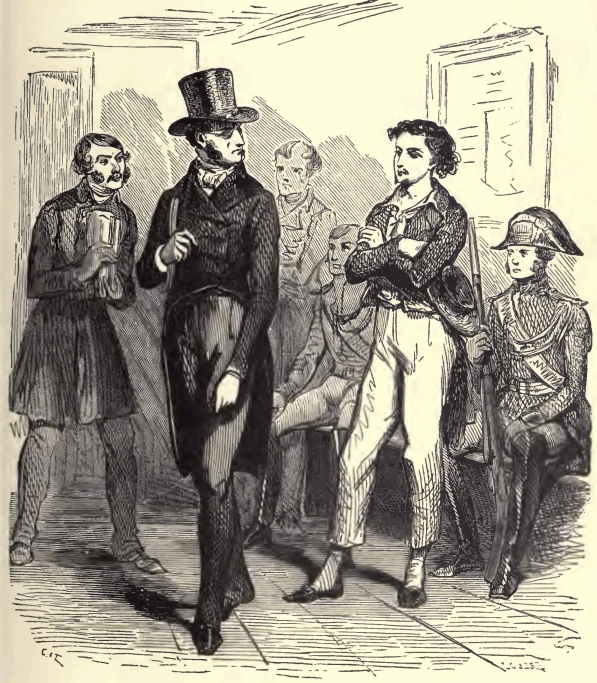
\includegraphics[width=\textwidth]{0099m.jpg}
\end{figure}

“Go on, sir,” said he.

“What would you have me say?”

“Give all the information in your power.”

“Tell me on which point you desire information, and I will tell all I
know; only,” added he, with a smile, “I warn you I know very little.”

“Have you served under the usurper?”

“I was about to be mustered into the Royal Marines when he fell.”

“It is reported your political opinions are extreme,” said Villefort,
who had never heard anything of the kind, but was not sorry to make
this inquiry, as if it were an accusation.

“My political opinions!” replied Dantès. “Alas, sir, I never had any
opinions. I am hardly nineteen; I know nothing; I have no part to play.
If I obtain the situation I desire, I shall owe it to M. Morrel. Thus
all my opinions—I will not say public, but private—are confined to
these three sentiments,—I love my father, I respect M. Morrel, and I
adore Mercédès. This, sir, is all I can tell you, and you see how
uninteresting it is.” As Dantès spoke, Villefort gazed at his ingenuous
and open countenance, and recollected the words of Renée, who, without
knowing who the culprit was, had besought his indulgence for him. With
the deputy’s knowledge of crime and criminals, every word the young man
uttered convinced him more and more of his innocence. This lad, for he
was scarcely a man,—simple, natural, eloquent with that eloquence of
the heart never found when sought for; full of affection for everybody,
because he was happy, and because happiness renders even the wicked
good—extended his affection even to his judge, spite of Villefort’s
severe look and stern accent. Dantès seemed full of kindness.

\textit{“Pardieu!”} said Villefort, “he is a noble fellow. I hope I shall gain
Renée’s favor easily by obeying the first command she ever imposed on
me. I shall have at least a pressure of the hand in public, and a sweet
kiss in private.” Full of this idea, Villefort’s face became so joyous,
that when he turned to Dantès, the latter, who had watched the change
on his physiognomy, was smiling also.

“Sir,” said Villefort, “have you any enemies, at least, that you know.”

“I have enemies?” replied Dantès; “my position is not sufficiently
elevated for that. As for my disposition, that is, perhaps, somewhat
too hasty; but I have striven to repress it. I have had ten or twelve
sailors under me, and if you question them, they will tell you that
they love and respect me, not as a father, for I am too young, but as
an elder brother.”

“But you may have excited jealousy. You are about to become captain at
nineteen—an elevated post; you are about to marry a pretty girl, who
loves you; and these two pieces of good fortune may have excited the
envy of someone.”

“You are right; you know men better than I do, and what you say may
possibly be the case, I confess; but if such persons are among my
acquaintances I prefer not to know it, because then I should be forced
to hate them.”

“You are wrong; you should always strive to see clearly around you. You
seem a worthy young man; I will depart from the strict line of my duty
to aid you in discovering the author of this accusation. Here is the
paper; do you know the writing?” As he spoke, Villefort drew the letter
from his pocket, and presented it to Dantès. Dantès read it. A cloud
passed over his brow as he said:

“No, monsieur, I do not know the writing, and yet it is tolerably
plain. Whoever did it writes well. I am very fortunate,” added he,
looking gratefully at Villefort, “to be examined by such a man as you;
for this envious person is a real enemy.” And by the rapid glance that
the young man’s eyes shot forth, Villefort saw how much energy lay hid
beneath this mildness.

“Now,” said the deputy, “answer me frankly, not as a prisoner to a
judge, but as one man to another who takes an interest in him, what
truth is there in the accusation contained in this anonymous letter?”
And Villefort threw disdainfully on his desk the letter Dantès had just
given back to him.

“None at all. I will tell you the real facts. I swear by my honor as a
sailor, by my love for Mercédès, by the life of my father——”

“Speak, monsieur,” said Villefort. Then, internally, “If Renée could
see me, I hope she would be satisfied, and would no longer call me a
decapitator.”

“Well, when we quitted Naples, Captain Leclere was attacked with a
brain fever. As we had no doctor on board, and he was so anxious to
arrive at Elba, that he would not touch at any other port, his disorder
rose to such a height, that at the end of the third day, feeling he was
dying, he called me to him. ‘My dear Dantès,’ said he, ‘swear to
perform what I am going to tell you, for it is a matter of the deepest
importance.’

“‘I swear, captain,’ replied I.

“‘Well, as after my death the command devolves on you as mate, assume
the command, and bear up for the Island of Elba, disembark at
Porto-Ferrajo, ask for the grand-marshal, give him this letter—perhaps
they will give you another letter, and charge you with a commission.
You will accomplish what I was to have done, and derive all the honor
and profit from it.’

“‘I will do it, captain; but perhaps I shall not be admitted to the
grand-marshal’s presence as easily as you expect?’

“‘Here is a ring that will obtain audience of him, and remove every
difficulty,’ said the captain. At these words he gave me a ring. It was
time—two hours after he was delirious; the next day he died.”

“And what did you do then?”

“What I ought to have done, and what everyone would have done in my
place. Everywhere the last requests of a dying man are sacred; but with
a sailor the last requests of his superior are commands. I sailed for
the Island of Elba, where I arrived the next day; I ordered everybody
to remain on board, and went on shore alone. As I had expected, I found
some difficulty in obtaining access to the grand-marshal; but I sent
the ring I had received from the captain to him, and was instantly
admitted. He questioned me concerning Captain Leclere’s death; and, as
the latter had told me, gave me a letter to carry on to a person in
Paris. I undertook it because it was what my captain had bade me do. I
landed here, regulated the affairs of the vessel, and hastened to visit
my affianced bride, whom I found more lovely than ever. Thanks to M.
Morrel, all the forms were got over; in a word I was, as I told you, at
my marriage feast; and I should have been married in an hour, and
tomorrow I intended to start for Paris, had I not been arrested on this
charge which you as well as I now see to be unjust.”

“Ah,” said Villefort, “this seems to me the truth. If you have been
culpable, it was imprudence, and this imprudence was in obedience to
the orders of your captain. Give up this letter you have brought from
Elba, and pass your word you will appear should you be required, and go
and rejoin your friends.

“I am free, then, sir?” cried Dantès joyfully.

“Yes; but first give me this letter.”

“You have it already, for it was taken from me with some others which I
see in that packet.”

“Stop a moment,” said the deputy, as Dantès took his hat and gloves.
“To whom is it addressed?”

\textit{“To Monsieur Noirtier, Rue Coq-Héron, Paris.”} Had a thunderbolt
fallen into the room, Villefort could not have been more stupefied. He
sank into his seat, and hastily turning over the packet, drew forth the
fatal letter, at which he glanced with an expression of terror.

“M. Noirtier, Rue Coq-Héron, No. 13,” murmured he, growing still paler.

“Yes,” said Dantès; “do you know him?”

“No,” replied Villefort; “a faithful servant of the king does not know
conspirators.”

\begin{figure}[ht]
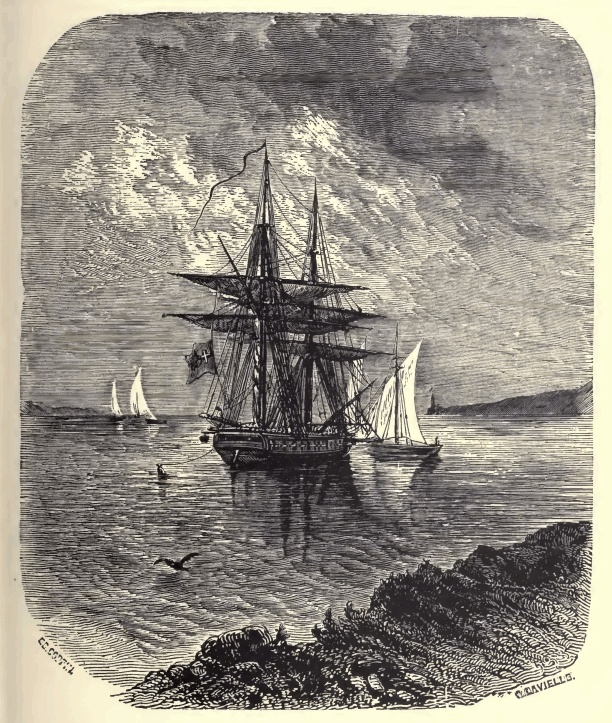
\includegraphics[width=\textwidth]{0103m.jpg}
\end{figure}

“It is a conspiracy, then?” asked Dantès, who after believing himself
free, now began to feel a tenfold alarm. “I have, however, already told
you, sir, I was entirely ignorant of the contents of the letter.”

“Yes; but you knew the name of the person to whom it was addressed,”
said Villefort.

“I was forced to read the address to know to whom to give it.”

“Have you shown this letter to anyone?” asked Villefort, becoming still
more pale.

“To no one, on my honor.”

“Everybody is ignorant that you are the bearer of a letter from the
Island of Elba, and addressed to M. Noirtier?”

“Everybody, except the person who gave it to me.”

“And that was too much, far too much,” murmured Villefort. Villefort’s
brow darkened more and more, his white lips and clenched teeth filled
Dantès with apprehension. After reading the letter, Villefort covered
his face with his hands.

“Oh,” said Dantès timidly, “what is the matter?” Villefort made no
answer, but raised his head at the expiration of a few seconds, and
again perused the letter.

“And you say that you are ignorant of the contents of this letter?”

“I give you my word of honor, sir,” said Dantès; “but what is the
matter? You are ill—shall I ring for assistance?—shall I call?”

“No,” said Villefort, rising hastily; “stay where you are. It is for me
to give orders here, and not you.”

“Monsieur,” replied Dantès proudly, “it was only to summon assistance
for you.”

“I want none; it was a temporary indisposition. Attend to yourself;
answer me.” Dantès waited, expecting a question, but in vain. Villefort
fell back on his chair, passed his hand over his brow, moist with
perspiration, and, for the third time, read the letter.

“Oh, if he knows the contents of this!” murmured he, “and that Noirtier
is the father of Villefort, I am lost!” And he fixed his eyes upon
Edmond as if he would have penetrated his thoughts.

“Oh, it is impossible to doubt it,” cried he, suddenly.

“In heaven’s name!” cried the unhappy young man, “if you doubt me,
question me; I will answer you.” Villefort made a violent effort, and
in a tone he strove to render firm:

“Sir,” said he, “I am no longer able, as I had hoped, to restore you
immediately to liberty; before doing so, I must consult the trial
justice; what my own feeling is you already know.”

“Oh, monsieur,” cried Dantès, “you have been rather a friend than a
judge.”

\begin{figure}[ht]
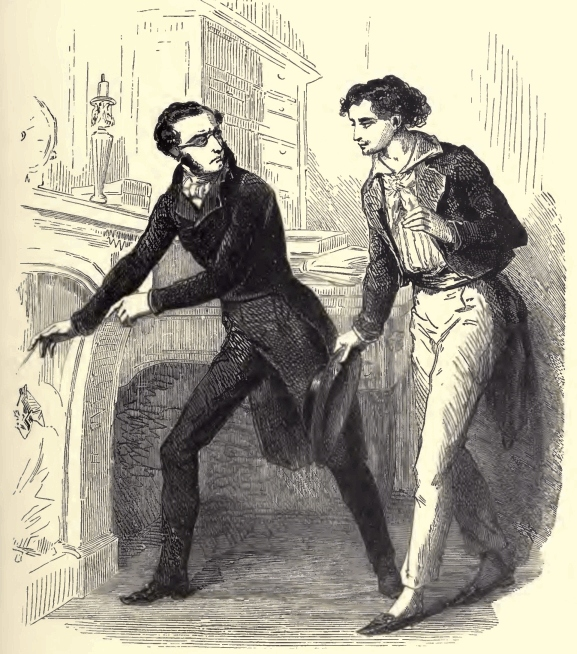
\includegraphics[width=\textwidth]{0105m.jpg}
\end{figure}

“Well, I must detain you some time longer, but I will strive to make it
as short as possible. The principal charge against you is this letter,
and you see——” Villefort approached the fire, cast it in, and waited
until it was entirely consumed.

“You see, I destroy it?”

“Oh,” exclaimed Dantès, “you are goodness itself.”

“Listen,” continued Villefort; “you can now have confidence in me after
what I have done.”

“Oh, command, and I will obey.”

“Listen; this is not a command, but advice I give you.”

“Speak, and I will follow your advice.”

“I shall detain you until this evening in the Palais de Justice. Should
anyone else interrogate you, say to him what you have said to me, but
do not breathe a word of this letter.”

“I promise.” It was Villefort who seemed to entreat, and the prisoner
who reassured him.

“You see,” continued he, glancing toward the grate, where fragments of
burnt paper fluttered in the flames, “the letter is destroyed; you and
I alone know of its existence; should you, therefore, be questioned,
deny all knowledge of it—deny it boldly, and you are saved.”

“Be satisfied; I will deny it.”

“It was the only letter you had?”

“It was.”

“Swear it.”

“I swear it.”

Villefort rang. A police agent entered. Villefort whispered some words
in his ear, to which the officer replied by a motion of his head.

“Follow him,” said Villefort to Dantès. Dantès saluted Villefort and
retired. Hardly had the door closed when Villefort threw himself
half-fainting into a chair.

“Alas, alas,” murmured he, “if the procureur himself had been at
Marseilles I should have been ruined. This accursed letter would have
destroyed all my hopes. Oh, my father, must your past career always
interfere with my successes?” Suddenly a light passed over his face, a
smile played round his set mouth, and his haggard eyes were fixed in
thought.

“This will do,” said he, “and from this letter, which might have ruined
me, I will make my fortune. Now to the work I have in hand.” And after
having assured himself that the prisoner was gone, the deputy procureur
hastened to the house of his betrothed.

\begin{figure}[ht]
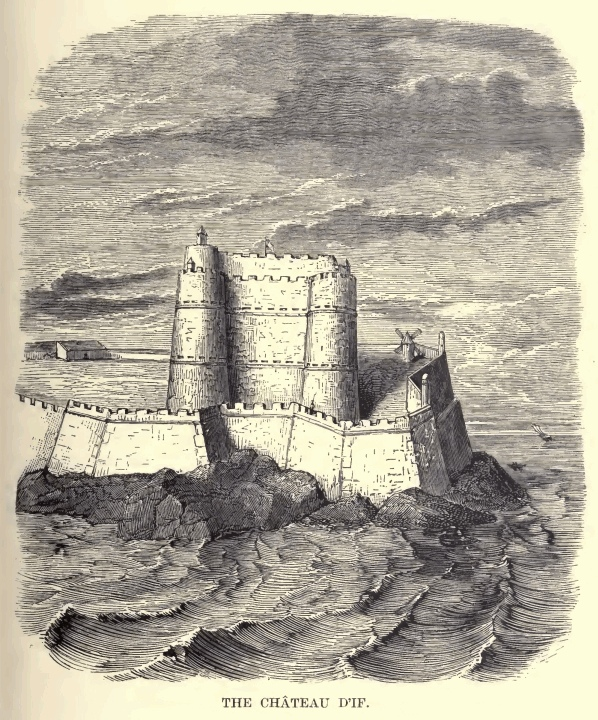
\includegraphics[width=\textwidth]{0107m.jpg}
\end{figure}

\printpagenotes*
\chapter{The Château d’If}

The commissary of police, as he traversed the antechamber, made a sign
to two gendarmes, who placed themselves one on Dantès’ right and the
other on his left. A door that communicated with the Palais de Justice
was opened, and they went through a long range of gloomy corridors,
whose appearance might have made even the boldest shudder. The Palais
de Justice communicated with the prison,—a sombre edifice, that from
its grated windows looks on the clock-tower of the Accoules. After
numberless windings, Dantès saw a door with an iron wicket. The
commissary took up an iron mallet and knocked thrice, every blow
seeming to Dantès as if struck on his heart. The door opened, the two
gendarmes gently pushed him forward, and the door closed with a loud
sound behind him. The air he inhaled was no longer pure, but thick and
mephitic,—he was in prison.

He was conducted to a tolerably neat chamber, but grated and barred,
and its appearance, therefore, did not greatly alarm him; besides, the
words of Villefort, who seemed to interest himself so much, resounded
still in his ears like a promise of freedom. It was four o’clock when
Dantès was placed in this chamber. It was, as we have said, the 1st of
March, and the prisoner was soon buried in darkness. The obscurity
augmented the acuteness of his hearing; at the slightest sound he rose
and hastened to the door, convinced they were about to liberate him,
but the sound died away, and Dantès sank again into his seat. At last,
about ten o’clock, and just as Dantès began to despair, steps were
heard in the corridor, a key turned in the lock, the bolts creaked, the
massy oaken door flew open, and a flood of light from two torches
pervaded the apartment.

By the torchlight Dantès saw the glittering sabres and carbines of four
gendarmes. He had advanced at first, but stopped at the sight of this
display of force.

“Are you come to fetch me?” asked he.

“Yes,” replied a gendarme.

“By the orders of the deputy procureur?”

“I believe so.” The conviction that they came from M. de Villefort
relieved all Dantès’ apprehensions; he advanced calmly, and placed
himself in the centre of the escort. A carriage waited at the door, the
coachman was on the box, and a police officer sat beside him.

“Is this carriage for me?” said Dantès.

“It is for you,” replied a gendarme.

Dantès was about to speak; but feeling himself urged forward, and
having neither the power nor the intention to resist, he mounted the
steps, and was in an instant seated inside between two gendarmes; the
two others took their places opposite, and the carriage rolled heavily
over the stones.

The prisoner glanced at the windows—they were grated; he had changed
his prison for another that was conveying him he knew not whither.
Through the grating, however, Dantès saw they were passing through the
Rue Caisserie, and by the Rue Saint-Laurent and the Rue Taramis, to the
quay. Soon he saw the lights of La Consigne.

The carriage stopped, the officer descended, approached the guardhouse,
a dozen soldiers came out and formed themselves in order; Dantès saw
the reflection of their muskets by the light of the lamps on the quay.

“Can all this force be summoned on my account?” thought he.

The officer opened the door, which was locked, and, without speaking a
word, answered Dantès’ question; for he saw between the ranks of the
soldiers a passage formed from the carriage to the port. The two
gendarmes who were opposite to him descended first, then he was ordered
to alight and the gendarmes on each side of him followed his example.
They advanced towards a boat, which a custom-house officer held by a
chain, near the quay.

The soldiers looked at Dantès with an air of stupid curiosity. In an
instant he was placed in the stern-sheets of the boat, between the
gendarmes, while the officer stationed himself at the bow; a shove sent
the boat adrift, and four sturdy oarsmen impelled it rapidly towards
the Pilon. At a shout from the boat, the chain that closes the mouth of
the port was lowered and in a second they were, as Dantès knew, in the
Frioul and outside the inner harbor.

The prisoner’s first feeling was of joy at again breathing the pure
air—for air is freedom; but he soon sighed, for he passed before La
Réserve, where he had that morning been so happy, and now through the
open windows came the laughter and revelry of a ball. Dantès folded his
hands, raised his eyes to heaven, and prayed fervently.

\begin{figure}[ht]
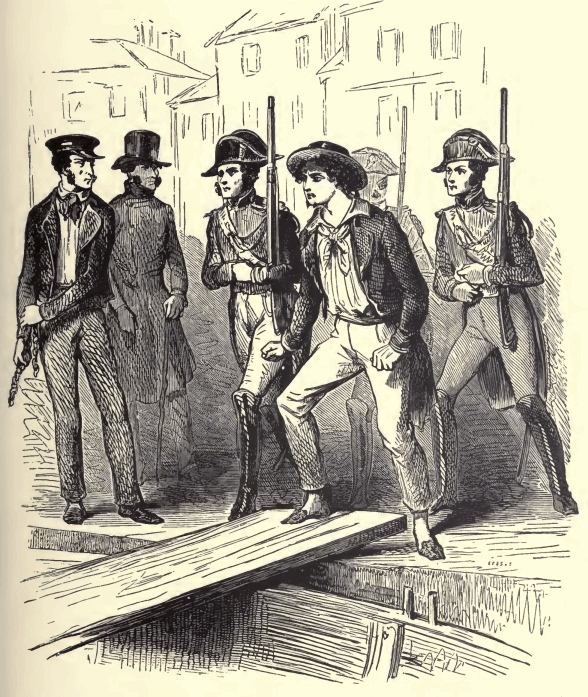
\includegraphics[width=\textwidth]{0111m.jpg}
\end{figure}

The boat continued her voyage. They had passed the Tête de Mort, were
now off the Anse du Pharo, and about to double the battery. This
manœuvre was incomprehensible to Dantès.

“Whither are you taking me?” asked he.

“You will soon know.”

“But still——”

“We are forbidden to give you any explanation.” Dantès, trained in
discipline, knew that nothing would be more absurd than to question
subordinates, who were forbidden to reply; and so he remained silent.

The most vague and wild thoughts passed through his mind. The boat they
were in could not make a long voyage; there was no vessel at anchor
outside the harbor; he thought, perhaps, they were going to leave him
on some distant point. He was not bound, nor had they made any attempt
to handcuff him; this seemed a good augury. Besides, had not the
deputy, who had been so kind to him, told him that provided he did not
pronounce the dreaded name of Noirtier, he had nothing to apprehend?
Had not Villefort in his presence destroyed the fatal letter, the only
proof against him?

He waited silently, striving to pierce through the darkness.

They had left the Ile Ratonneau, where the lighthouse stood, on the
right, and were now opposite the Point des Catalans. It seemed to the
prisoner that he could distinguish a feminine form on the beach, for it
was there Mercédès dwelt. How was it that a presentiment did not warn
Mercédès that her lover was within three hundred yards of her?

One light alone was visible; and Dantès saw that it came from Mercédès’
chamber. Mercédès was the only one awake in the whole settlement. A
loud cry could be heard by her. But pride restrained him and he did not
utter it. What would his guards think if they heard him shout like a
madman?

He remained silent, his eyes fixed upon the light; the boat went on,
but the prisoner thought only of Mercédès. An intervening elevation of
land hid the light. Dantès turned and perceived that they had got out
to sea. While he had been absorbed in thought, they had shipped their
oars and hoisted sail; the boat was now moving with the wind.

In spite of his repugnance to address the guards, Dantès turned to the
nearest gendarme, and taking his hand,

“Comrade,” said he, “I adjure you, as a Christian and a soldier, to
tell me where we are going. I am Captain Dantès, a loyal Frenchman,
thought accused of treason; tell me where you are conducting me, and I
promise you on my honor I will submit to my fate.”

The gendarme looked irresolutely at his companion, who returned for
answer a sign that said, “I see no great harm in telling him now,” and
the gendarme replied:

“You are a native of Marseilles, and a sailor, and yet you do not know
where you are going?”

“On my honor, I have no idea.”

“Have you no idea whatever?”

“None at all.”

“That is impossible.”

“I swear to you it is true. Tell me, I entreat.”

“But my orders.”

“Your orders do not forbid your telling me what I must know in ten
minutes, in half an hour, or an hour. You see I cannot escape, even if
I intended.”

“Unless you are blind, or have never been outside the harbor, you must
know.”

“I do not.”

“Look round you then.” Dantès rose and looked forward, when he saw rise
within a hundred yards of him the black and frowning rock on which
stands the Château d’If. This gloomy fortress, which has for more than
three hundred years furnished food for so many wild legends, seemed to
Dantès like a scaffold to a malefactor.

“The Château d’If?” cried he, “what are we going there for?”

The gendarme smiled.

“I am not going there to be imprisoned,” said Dantès; “it is only used
for political prisoners. I have committed no crime. Are there any
magistrates or judges at the Château d’If?”

“There are only,” said the gendarme, “a governor, a garrison, turnkeys,
and good thick walls. Come, come, do not look so astonished, or you
will make me think you are laughing at me in return for my good
nature.”

Dantès pressed the gendarme’s hand as though he would crush it.

“You think, then,” said he, “that I am taken to the Château d’If to be
imprisoned there?”

“It is probable; but there is no occasion to squeeze so hard.”

“Without any inquiry, without any formality?”

“All the formalities have been gone through; the inquiry is already
made.”

“And so, in spite of M. de Villefort’s promises?”

“I do not know what M. de Villefort promised you,” said the gendarme,
“but I know we are taking you to the Château d’If. But what are you
doing? Help, comrades, help!”

By a rapid movement, which the gendarme’s practiced eye had perceived,
Dantès sprang forward to precipitate himself into the sea; but four
vigorous arms seized him as his feet quitted the bottom of the boat. He
fell back cursing with rage.

“Good!” said the gendarme, placing his knee on his chest; “this is the
way you keep your word as a sailor! Believe soft-spoken gentlemen
again! Hark ye, my friend, I have disobeyed my first order, but I will
not disobey the second; and if you move, I will blow your brains out.”
And he levelled his carbine at Dantès, who felt the muzzle against his
temple.

For a moment the idea of struggling crossed his mind, and of so ending
the unexpected evil that had overtaken him. But he bethought him of M.
de Villefort’s promise; and, besides, death in a boat from the hand of
a gendarme seemed too terrible. He remained motionless, but gnashing
his teeth and wringing his hands with fury.

At this moment the boat came to a landing with a violent shock. One of
the sailors leaped on shore, a cord creaked as it ran through a pulley,
and Dantès guessed they were at the end of the voyage, and that they
were mooring the boat.

His guards, taking him by the arms and coat-collar, forced him to rise,
and dragged him towards the steps that lead to the gate of the
fortress, while the police officer carrying a musket with fixed bayonet
followed behind.

Dantès made no resistance; he was like a man in a dream; he saw
soldiers drawn up on the embankment; he knew vaguely that he was
ascending a flight of steps; he was conscious that he passed through a
door, and that the door closed behind him; but all this indistinctly as
through a mist. He did not even see the ocean, that terrible barrier
against freedom, which the prisoners look upon with utter despair.

They halted for a minute, during which he strove to collect his
thoughts. He looked around; he was in a court surrounded by high walls;
he heard the measured tread of sentinels, and as they passed before the
light he saw the barrels of their muskets shine.

They waited upwards of ten minutes. Certain Dantès could not escape,
the gendarmes released him. They seemed awaiting orders. The orders
came.

“Where is the prisoner?” said a voice.

“Here,” replied the gendarmes.

“Let him follow me; I will take him to his cell.”

“Go!” said the gendarmes, thrusting Dantès forward.

The prisoner followed his guide, who led him into a room almost under
ground, whose bare and reeking walls seemed as though impregnated with
tears; a lamp placed on a stool illumined the apartment faintly, and
showed Dantès the features of his conductor, an under-jailer,
ill-clothed, and of sullen appearance.

\begin{figure}[h]
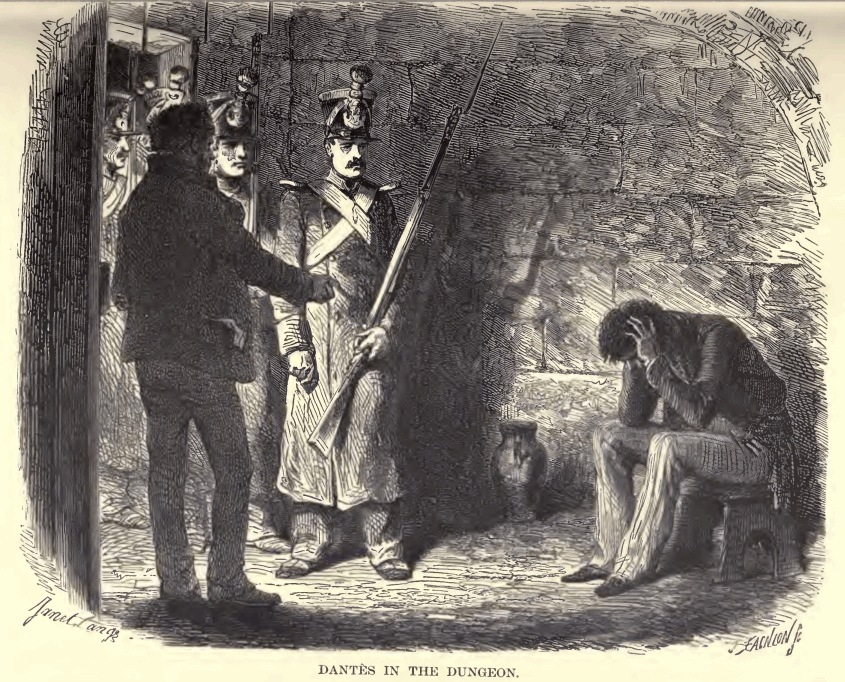
\includegraphics[width=\textwidth]{0113m.jpg}
\end{figure}

“Here is your chamber for tonight,” said he. “It is late, and the
governor is asleep. Tomorrow, perhaps, he may change you. In the
meantime there is bread, water, and fresh straw; and that is all a
prisoner can wish for. Goodnight.” And before Dantès could open his
mouth—before he had noticed where the jailer placed his bread or the
water—before he had glanced towards the corner where the straw was, the
jailer disappeared, taking with him the lamp and closing the door,
leaving stamped upon the prisoner’s mind the dim reflection of the
dripping walls of his dungeon.

Dantès was alone in darkness and in silence—cold as the shadows that he
felt breathe on his burning forehead. With the first dawn of day the
jailer returned, with orders to leave Dantès where he was. He found the
prisoner in the same position, as if fixed there, his eyes swollen with
weeping. He had passed the night standing, and without sleep. The
jailer advanced; Dantès appeared not to perceive him. He touched him on
the shoulder. Edmond started.

“Have you not slept?” said the jailer.

“I do not know,” replied Dantès. The jailer stared.

“Are you hungry?” continued he.

“I do not know.”

“Do you wish for anything?”

“I wish to see the governor.”

The jailer shrugged his shoulders and left the chamber.

Dantès followed him with his eyes, and stretched forth his hands
towards the open door; but the door closed. All his emotion then burst
forth; he cast himself on the ground, weeping bitterly, and asking
himself what crime he had committed that he was thus punished.

The day passed thus; he scarcely tasted food, but walked round and
round the cell like a wild beast in its cage. One thought in particular
tormented him: namely, that during his journey hither he had sat so
still, whereas he might, a dozen times, have plunged into the sea, and,
thanks to his powers of swimming, for which he was famous, have gained
the shore, concealed himself until the arrival of a Genoese or Spanish
vessel, escaped to Spain or Italy, where Mercédès and his father could
have joined him. He had no fears as to how he should live—good seamen
are welcome everywhere. He spoke Italian like a Tuscan, and Spanish
like a Castilian; he would have been free, and happy with Mercédès and
his father, whereas he was now confined in the Château d’If, that
impregnable fortress, ignorant of the future destiny of his father and
Mercédès; and all this because he had trusted to Villefort’s promise.
The thought was maddening, and Dantès threw himself furiously down on
his straw. The next morning at the same hour, the jailer came again.

“Well,” said the jailer, “are you more reasonable today?” Dantès made
no reply.

“Come, cheer up; is there anything that I can do for you?”

“I wish to see the governor.”

“I have already told you it was impossible.”

“Why so?”

“Because it is against prison rules, and prisoners must not even ask
for it.”

“What is allowed, then?”

“Better fare, if you pay for it, books, and leave to walk about.”

“I do not want books, I am satisfied with my food, and do not care to
walk about; but I wish to see the governor.”

“If you worry me by repeating the same thing, I will not bring you any
more to eat.”

“Well, then,” said Edmond, “if you do not, I shall die of hunger—that
is all.”

The jailer saw by his tone he would be happy to die; and as every
prisoner is worth ten sous a day to his jailer, he replied in a more
subdued tone.

“What you ask is impossible; but if you are very well behaved you will
be allowed to walk about, and some day you will meet the governor, and
if he chooses to reply, that is his affair.”

“But,” asked Dantès, “how long shall I have to wait?”

“Ah, a month—six months—a year.”

“It is too long a time. I wish to see him at once.”

“Ah,” said the jailer, “do not always brood over what is impossible, or
you will be mad in a fortnight.”

“You think so?”

“Yes; we have an instance here; it was by always offering a million of
francs to the governor for his liberty that an abbé became mad, who was
in this chamber before you.”

\begin{figure}[h]
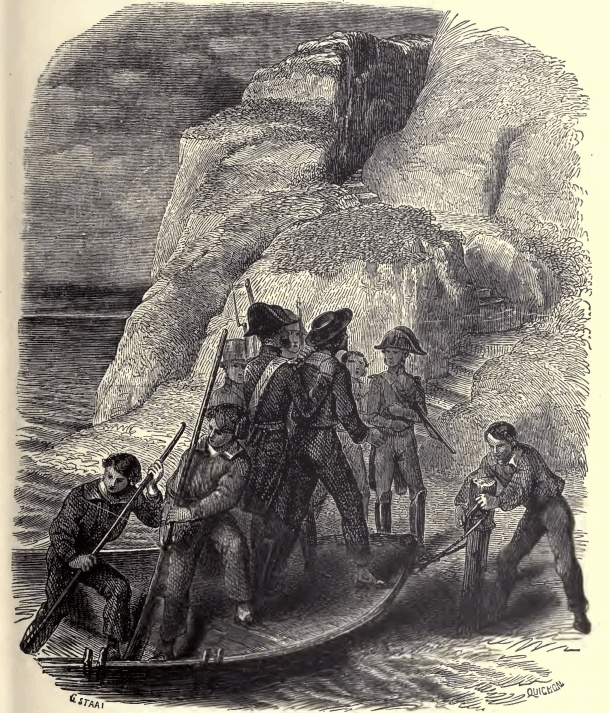
\includegraphics[width=\textwidth]{0119m.jpg}
\end{figure}

“How long has he left it?”

“Two years.”

“Was he liberated, then?”

“No; he was put in a dungeon.”

“Listen!” said Dantès. “I am not an abbé, I am not mad; perhaps I shall
be, but at present, unfortunately, I am not. I will make you another
offer.”

“What is that?”

“I do not offer you a million, because I have it not; but I will give
you a hundred crowns if, the first time you go to Marseilles, you will
seek out a young girl named Mercédès, at the Catalans, and give her two
lines from me.”

\begin{figure}[h]
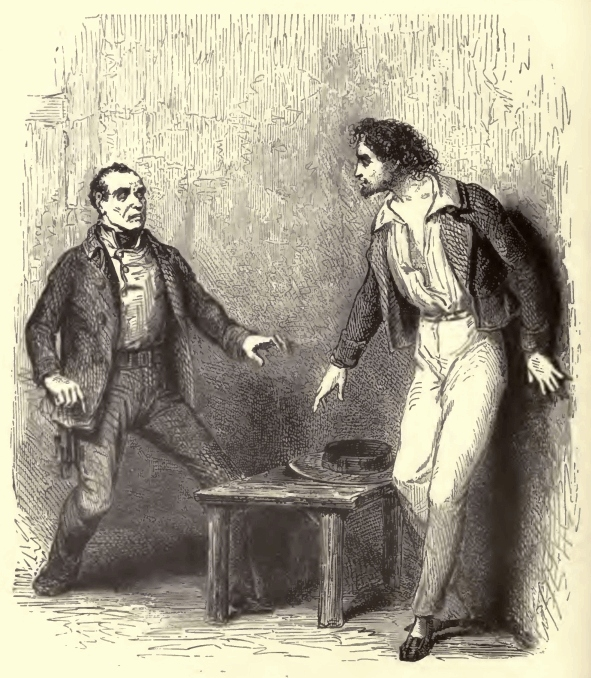
\includegraphics[width=\textwidth]{0120m.jpg}
\end{figure}

“If I took them, and were detected, I should lose my place, which is
worth two thousand francs a year; so that I should be a great fool to
run such a risk for three hundred.”

“Well,” said Dantès, “mark this; if you refuse at least to tell
Mercédès I am here, I will some day hide myself behind the door, and
when you enter I will dash out your brains with this stool.”

“Threats!” cried the jailer, retreating and putting himself on the
defensive; “you are certainly going mad. The abbé began like you, and
in three days you will be like him, mad enough to tie up; but,
fortunately, there are dungeons here.”

Dantès whirled the stool round his head.

“All right, all right,” said the jailer; “all right, since you will
have it so. I will send word to the governor.”

“Very well,” returned Dantès, dropping the stool and sitting on it as
if he were in reality mad. The jailer went out, and returned in an
instant with a corporal and four soldiers.

“By the governor’s orders,” said he, “conduct the prisoner to the tier
beneath.”

“To the dungeon, then,” said the corporal.

“Yes; we must put the madman with the madmen.” The soldiers seized
Dantès, who followed passively.

He descended fifteen steps, and the door of a dungeon was opened, and
he was thrust in. The door closed, and Dantès advanced with
outstretched hands until he touched the wall; he then sat down in the
corner until his eyes became accustomed to the darkness. The jailer was
right; Dantès wanted but little of being utterly mad.

\printpagenotes*
\chapter{State Of Germany Until The Barbarians.}
\section{Part \thesection.}

\textit{The State Of Germany Till The Invasion Of The Barbarians In The
Time Of The Emperor Decius.}
\vspace{\onelineskip}

The government and religion of Persia have deserved some notice,
from their connection with the decline and fall of the Roman
empire. We shall occasionally mention the Scythian or Sarmatian
tribes,\textsuperscript{1001} which, with their arms and horses, their flocks and
herds, their wives and families, wandered over the immense plains
which spread themselves from the Caspian Sea to the Vistula, from
the confines of Persia to those of Germany. But the warlike
Germans, who first resisted, then invaded, and at length
overturned the Western monarchy of Rome, will occupy a much more
important place in this history, and possess a stronger, and, if
we may use the expression, a more domestic, claim to our
attention and regard. The most civilized nations of modern Europe
issued from the woods of Germany; and in the rude institutions of
those barbarians we may still distinguish the original principles
of our present laws and manners. In their primitive state of
simplicity and independence, the Germans were surveyed by the
discerning eye, and delineated by the masterly pencil, of
Tacitus,\textsuperscript{1002} the first of historians who applied the science of
philosophy to the study of facts. The expressive conciseness of
his descriptions has served to exercise the diligence of
innumerable antiquarians, and to excite the genius and
penetration of the philosophic historians of our own times. The
subject, however various and important, has already been so
frequently, so ably, and so successfully discussed, that it is
now grown familiar to the reader, and difficult to the writer. We
shall therefore content ourselves with observing, and indeed with
repeating, some of the most important circumstances of climate,
of manners, and of institutions, which rendered the wild
barbarians of Germany such formidable enemies to the Roman power.

\pagenote[1001]{The Scythians, even according to the ancients,
are not Sarmatians. It may be doubted whether Gibbon intended to
confound them.—M. ——The Greeks, after having divided the world
into Greeks and barbarians. divided the barbarians into four
great classes, the Celts, the Scythians, the Indians, and the
Ethiopians. They called Celts all the inhabitants of Gaul.
Scythia extended from the Baltic Sea to the Lake Aral: the people
enclosed in the angle to the north-east, between Celtica and
Scythia, were called Celto-Scythians, and the Sarmatians were
placed in the southern part of that angle. But these names of
Celts, of Scythians, of Celto-Scythians, and Sarmatians, were
invented, says Schlozer, by the profound cosmographical ignorance
of the Greeks, and have no real ground; they are purely
geographical divisions, without any relation to the true
affiliation of the different races. Thus all the inhabitants of
Gaul are called Celts by most of the ancient writers; yet Gaul
contained three totally distinct nations, the Belgæ, the
Aquitani, and the Gauls, properly so called. Hi omnes lingua
institutis, legibusque inter se differunt. Cæsar. Com. c. i. It
is thus the Turks call all Europeans Franks. Schlozer, Allgemeine
Nordische Geschichte, p. 289. 1771. Bayer (de Origine et priscis
Sedibus Scytharum, in Opusc. p. 64) says, Primus eorum, de quibus
constat, Ephorus, in quarto historiarum libro, orbem terrarum
inter Scythas, Indos, Æthiopas et Celtas divisit. Fragmentum ejus
loci Cosmas Indicopleustes in topographia Christiana, f. 148,
conservavit. Video igitur Ephorum, cum locorum positus per certa
capita distribuere et explicare constitueret, insigniorum nomina
gentium vastioribus spatiis adhibuisse, nulla mala fraude et
successu infelici. Nam Ephoro quoquomodo dicta pro exploratis
habebant Græci plerique et Romani: ita gliscebat error
posteritate. Igitur tot tamque diversæ stirpis gentes non modo
intra communem quandam regionem definitæ, unum omnes Scytharum
nomen his auctoribus subierunt, sed etiam ab illa regionis
adpellatione in eandem nationem sunt conflatæ. Sic Cimmeriorum
res cum Scythicis, Scytharum cum Sarmaticis, Russicis, Hunnicis,
Tataricis commiscentur.—G.}

\pagenote[1002]{The Germania of Tacitus has been a fruitful
source of hypothesis to the ingenuity of modern writers, who have
endeavored to account for the form of the work and the views of
the author. According to Luden, (Geschichte des T. V. i. 432, and
note,) it contains the unfinished and disarranged for a larger
work. An anonymous writer, supposed by Luden to be M. Becker,
conceives that it was intended as an episode in his larger
history. According to M. Guizot, “Tacite a peint les Germains
comme Montaigne et Rousseau les sauvages, dans un acces d’humeur
contre sa patrie: son livre est une satire des mœurs Romaines,
l’eloquente boutade d’un patriote philosophe qui veut voir la
vertu la, ou il ne rencontre pas la mollesse honteuse et la
depravation savante d’une vielle societe.” Hist. de la
Civilisation Moderne, i. 258.—M.}

Ancient Germany, excluding from its independent limits the
province westward of the Rhine, which had submitted to the Roman
yoke, extended itself over a third part of Europe.\textsuperscript{1} Almost the
whole of modern Germany, Denmark, Norway, Sweden, Finland,
Livonia, Prussia, and the greater part of Poland, were peopled by
the various tribes of one great nation, whose complexion,
manners, and language denoted a common origin, and preserved a
striking resemblance. On the west, ancient Germany was divided by
the Rhine from the Gallic, and on the south, by the Danube, from
the Illyrian, provinces of the empire. A ridge of hills, rising
from the Danube, and called the Carpathian Mountains, covered
Germany on the side of Dacia or Hungary. The eastern frontier was
faintly marked by the mutual fears of the Germans and the
Sarmatians, and was often confounded by the mixture of warring
and confederating tribes of the two nations. In the remote
darkness of the north, the ancients imperfectly descried a frozen
ocean that lay beyond the Baltic Sea, and beyond the Peninsula,
or islands\textsuperscript{1001a} of Scandinavia.

\pagenote[1]{Germany was not of such vast extent. It is from
Cæsar, and more particularly from Ptolemy, (says Gatterer,) that
we can know what was the state of ancient Germany before the wars
with the Romans had changed the positions of the tribes. Germany,
as changed by these wars, has been described by Strabo, Pliny,
and Tacitus. Germany, properly so called, was bounded on the west
by the Rhine, on the east by the Vistula, on the north by the
southern point of Norway, by Sweden, and Esthonia. On the south,
the Maine and the mountains to the north of Bohemia formed the
limits. Before the time of Cæsar, the country between the Maine
and the Danube was partly occupied by the Helvetians and other
Gauls, partly by the Hercynian forest but, from the time of Cæsar
to the great migration, these boundaries were advanced as far as
the Danube, or, what is the same thing, to the Suabian Alps,
although the Hercynian forest still occupied, from north to
south, a space of nine days’ journey on both banks of the Danube.
“Gatterer, Versuch einer all-gemeinen Welt-Geschichte,” p. 424,
edit. de 1792. This vast country was far from being inhabited by
a single nation divided into different tribes of the same origin.
We may reckon three principal races, very distinct in their
language, their origin, and their customs. 1. To the east, the
Slaves or Vandals. 2. To the west, the Cimmerians or Cimbri. 3.
Between the Slaves and Cimbrians, the Germans, properly so
called, the Suevi of Tacitus. The South was inhabited, before
Julius Cæsar, by nations of Gaulish origin, afterwards by the
Suevi.—G. On the position of these nations, the German
antiquaries differ. I. The Slaves, or Sclavonians, or Wendish
tribes, according to Schlozer, were originally settled in parts
of Germany unknown to the Romans, Mecklenburgh, Pomerania,
Brandenburgh, Upper Saxony; and Lusatia. According to Gatterer,
they remained to the east of the Theiss, the Niemen, and the
Vistula, till the third century. The Slaves, according to
Procopius and Jornandes, formed three great divisions. 1. The
Venedi or Vandals, who took the latter name, (the Wenden,) having
expelled the Vandals, properly so called, (a Suevian race, the
conquerors of Africa,) from the country between the Memel and the
Vistula. 2. The Antes, who inhabited between the Dneister and the
Dnieper. 3. The Sclavonians, properly so called, in the north of
Dacia. During the great migration, these races advanced into
Germany as far as the Saal and the Elbe. The Sclavonian language
is the stem from which have issued the Russian, the Polish, the
Bohemian, and the dialects of Lusatia, of some parts of the duchy
of Luneburgh, of Carniola, Carinthia, and Styria, \&c.; those of
Croatia, Bosnia, and Bulgaria. Schlozer, Nordische Geschichte, p.
323, 335. II. The Cimbric race. Adelung calls by this name all
who were not Suevi. This race had passed the Rhine, before the
time of Cæsar, occupied Belgium, and are the Belgæ of Cæsar and
Pliny. The Cimbrians also occupied the Isle of Jutland. The Cymri
of Wales and of Britain are of this race. Many tribes on the
right bank of the Rhine, the Guthini in Jutland, the Usipeti in
Westphalia, the Sigambri in the duchy of Berg, were German
Cimbrians. III. The Suevi, known in very early times by the
Romans, for they are mentioned by L. Corn. Sisenna, who lived 123
years before Christ, (Nonius v. Lancea.) This race, the real
Germans, extended to the Vistula, and from the Baltic to the
Hercynian forest. The name of Suevi was sometimes confined to a
single tribe, as by Cæsar to the Catti. The name of the Suevi has
been preserved in Suabia. These three were the principal races
which inhabited Germany; they moved from east to west, and are
the parent stem of the modern natives. But northern Europe,
according to Schlozer, was not peopled by them alone; other
races, of different origin, and speaking different languages,
have inhabited and left descendants in these countries. The
German tribes called themselves, from very remote times, by the
generic name of Teutons, (Teuten, Deutschen,) which Tacitus
derives from that of one of their gods, Tuisco. It appears more
probable that it means merely men, people. Many savage nations
have given themselves no other name. Thus the Laplanders call
themselves Almag, people; the Samoiedes Nilletz, Nissetsch, men,
\&c. As to the name of Germans, (Germani,) Cæsar found it in use
in Gaul, and adopted it as a word already known to the Romans.
Many of the learned (from a passage of Tacitus, de Mor Germ. c.
2) have supposed that it was only applied to the Teutons after
Cæsar’s time; but Adelung has triumphantly refuted this opinion.
The name of Germans is found in the Fasti Capitolini. See Gruter,
Iscrip. 2899, in which the consul Marcellus, in the year of Rome
531, is said to have defeated the Gauls, the Insubrians, and the
Germans, commanded by Virdomar. See Adelung, Ælt. Geschichte der
Deutsch, p. 102.—Compressed from G.}

\pagenote[1001a]{The modern philosophers of Sweden seem agreed
that the waters of the Baltic gradually sink in a regular
proportion, which they have ventured to estimate at half an inch
every year. Twenty centuries ago the flat country of Scandinavia
must have been covered by the sea; while the high lands rose
above the waters, as so many islands of various forms and
dimensions. Such, indeed, is the notion given us by Mela, Pliny,
and Tacitus, of the vast countries round the Baltic. See in the
Bibliotheque Raisonnee, tom. xl. and xlv. a large abstract of
Dalin’s History of Sweden, composed in the Swedish language. *
Note: Modern geologists have rejected this theory of the
depression of the Baltic, as inconsistent with recent
observation. The considerable changes which have taken place on
its shores, Mr. Lyell, from actual observation now decidedly
attributes to the regular and uniform elevation of the
land.—Lyell’s Geology, b. ii. c. 17—M.}

Some ingenious writers\textsuperscript{2} have suspected that Europe was much
colder formerly than it is at present; and the most ancient
descriptions of the climate of Germany tend exceedingly to
confirm their theory. The general complaints of intense frost and
eternal winter are perhaps little to be regarded, since we have
no method of reducing to the accurate standard of the
thermometer, the feelings, or the expressions, of an orator born
in the happier regions of Greece or Asia. But I shall select two
remarkable circumstances of a less equivocal nature. 1. The great
rivers which covered the Roman provinces, the Rhine and the
Danube, were frequently frozen over, and capable of supporting
the most enormous weights. The barbarians, who often chose that
severe season for their inroads, transported, without
apprehension or danger, their numerous armies, their cavalry, and
their heavy wagons, over a vast and solid bridge of ice.\textsuperscript{3} Modern
ages have not presented an instance of a like phenomenon. 2. The
reindeer, that useful animal, from whom the savage of the North
derives the best comforts of his dreary life, is of a
constitution that supports, and even requires, the most intense
cold. He is found on the rock of Spitzberg, within ten degrees of
the Pole; he seems to delight in the snows of Lapland and
Siberia: but at present he cannot subsist, much less multiply, in
any country to the south of the Baltic.\textsuperscript{4} In the time of Cæsar
the reindeer, as well as the elk and the wild bull, was a native
of the Hercynian forest, which then overshadowed a great part of
Germany and Poland.\textsuperscript{5} The modern improvements sufficiently
explain the causes of the diminution of the cold. These immense
woods have been gradually cleared, which intercepted from the
earth the rays of the sun.\textsuperscript{6} The morasses have been drained, and,
in proportion as the soil has been cultivated, the air has become
more temperate. Canada, at this day, is an exact picture of
ancient Germany. Although situated in the same parallel with the
finest provinces of France and England, that country experiences
the most rigorous cold. The reindeer are very numerous, the
ground is covered with deep and lasting snow, and the great river
of St. Lawrence is regularly frozen, in a season when the waters
of the Seine and the Thames are usually free from ice.\textsuperscript{7}

\pagenote[2]{In particular, Mr. Hume, the Abbé du Bos, and M.
Pelloutier. Hist. des Celtes, tom. i.}

\pagenote[3]{Diodorus Siculus, l. v. p. 340, edit. Wessel.
Herodian, l. vi. p. 221. Jornandes, c. 55. On the banks of the
Danube, the wine, when brought to table, was frequently frozen
into great lumps, frusta vini. Ovid. Epist. ex Ponto, l. iv. 7,
9, 10. Virgil. Georgic. l. iii. 355. The fact is confirmed by a
soldier and a philosopher, who had experienced the intense cold
of Thrace. See Xenophon, Anabasis, l. vii. p. 560, edit.
Hutchinson. Note: The Danube is constantly frozen over. At Pesth
the bridge is usually taken up, and the traffic and communication
between the two banks carried on over the ice. The Rhine is
likewise in many parts passable at least two years out of five.
Winter campaigns are so unusual, in modern warfare, that I
recollect but one instance of an army crossing either river on
the ice. In the thirty years’ war, (1635,) Jan van Werth, an
Imperialist partisan, crossed the Rhine from Heidelberg on the
ice with 5000 men, and surprised Spiers. Pichegru’s memorable
campaign, (1794-5,) when the freezing of the Meuse and Waal
opened Holland to his conquests, and his cavalry and artillery
attacked the ships frozen in, on the Zuyder Zee, was in a winter
of unprecedented severity.—M. 1845.}

\pagenote[4]{Buffon, Histoire Naturelle, tom. xii. p. 79, 116.}

\pagenote[5]{Cæsar de Bell. Gallic. vi. 23, \&c. The most
inquisitive of the Germans were ignorant of its utmost limits,
although some of them had travelled in it more than sixty days’
journey. * Note: The passage of Cæsar, “parvis renonum tegumentis
utuntur,” is obscure, observes Luden, (Geschichte des Teutschen
Volkes,) and insufficient to prove the reindeer to have existed
in Germany. It is supported however, by a fragment of Sallust.
Germani intectum rhenonibus corpus tegunt.—M. It has been
suggested to me that Cæsar (as old Gesner supposed) meant the
reindeer in the following description. Est bos cervi figura cujus
a media fronte inter aures unum cornu existit, excelsius magisque
directum (divaricatum, qu?) his quæ nobis nota sunt cornibus. At
ejus summo, sicut palmæ, rami quam late diffunduntur. Bell.
vi.—M. 1845.}

\pagenote[6]{Cluverius (Germania Antiqua, l. iii. c. 47)
investigates the small and scattered remains of the Hercynian
wood.}

\pagenote[7]{Charlevoix, Histoire du Canada.}

It is difficult to ascertain, and easy to exaggerate, the
influence of the climate of ancient Germany over the minds and
bodies of the natives. Many writers have supposed, and most have
allowed, though, as it should seem, without any adequate proof,
that the rigorous cold of the North was favorable to long life
and generative vigor, that the women were more fruitful, and the
human species more prolific, than in warmer or more temperate
climates.\textsuperscript{8} We may assert, with greater confidence, that the keen
air of Germany formed the large and masculine limbs of the
natives, who were, in general, of a more lofty stature than the
people of the South,\textsuperscript{9} gave them a kind of strength better
adapted to violent exertions than to patient labor, and inspired
them with constitutional bravery, which is the result of nerves
and spirits. The severity of a winter campaign, that chilled the
courage of the Roman troops, was scarcely felt by these hardy
children of the North,\textsuperscript{10} who, in their turn, were unable to
resist the summer heats, and dissolved away in languor and
sickness under the beams of an Italian sun.\textsuperscript{11}

\pagenote[8]{Olaus Rudbeck asserts that the Swedish women often
bear ten or twelve children, and not uncommonly twenty or thirty;
but the authority of Rudbeck is much to be suspected.}

\pagenote[9]{In hos artus, in hæc corpora, quæ miramur,
excrescunt. Tæit Germania, 3, 20. Cluver. l. i. c. 14.}

\pagenote[10]{Plutarch. in Mario. The Cimbri, by way of
amusement, often did down mountains of snow on their broad
shields.}

\pagenote[11]{The Romans made war in all climates, and by their
excellent discipline were in a great measure preserved in health
and vigor. It may be remarked, that man is the only animal which
can live and multiply in every country from the equator to the
poles. The hog seems to approach the nearest to our species in
that privilege.}

\section{Part \thesection.}

There is not anywhere upon the globe a large tract of country,
which we have discovered destitute of inhabitants, or whose first
population can be fixed with any degree of historical certainty.
And yet, as the most philosophic minds can seldom refrain from
investigating the infancy of great nations, our curiosity
consumes itself in toilsome and disappointed efforts. When
Tacitus considered the purity of the German blood, and the
forbidding aspect of the country, he was disposed to pronounce
those barbarians \textit{Indigenæ}, or natives of the soil. We may allow
with safety, and perhaps with truth, that ancient Germany was not
originally peopled by any foreign colonies already formed into a
political society;\textsuperscript{12} but that the name and nation received their
existence from the gradual union of some wandering savages of the
Hercynian woods. To assert those savages to have been the
spontaneous production of the earth which they inhabited would be
a rash inference, condemned by religion, and unwarranted by
reason.

\pagenote[12]{Facit. Germ. c. 3. The emigration of the Gauls
followed the course of the Danube, and discharged itself on
Greece and Asia. Tacitus could discover only one inconsiderable
tribe that retained any traces of a Gallic origin. * Note: The
Gothini, who must not be confounded with the Gothi, a Suevian
tribe. In the time of Cæsar many other tribes of Gaulish origin
dwelt along the course of the Danube, who could not long resist
the attacks of the Suevi. The Helvetians, who dwelt on the
borders of the Black Forest, between the Maine and the Danube,
had been expelled long before the time of Cæsar. He mentions also
the Volci Tectosagi, who came from Languedoc and settled round
the Black Forest. The Boii, who had penetrated into that forest,
and also have left traces of their name in Bohemia, were subdued
in the first century by the Marcomanni. The Boii settled in
Noricum, were mingled afterwards with the Lombards, and received
the name of Boio Arii (Bavaria) or Boiovarii: var, in some German
dialects, appearing to mean remains, descendants. Compare Malte
B-m, Geography, vol. i. p. 410, edit 1832—M.}

Such rational doubt is but ill suited with the genius of popular
vanity. Among the nations who have adopted the Mosaic history of
the world, the ark of Noah has been of the same use, as was
formerly to the Greeks and Romans the siege of Troy. On a narrow
basis of acknowledged truth, an immense but rude superstructure
of fable has been erected; and the wild Irishman,\textsuperscript{13} as well as
the wild Tartar,\textsuperscript{14} could point out the individual son of Japhet,
from whose loins his ancestors were lineally descended. The last
century abounded with antiquarians of profound learning and easy
faith, who, by the dim light of legends and traditions, of
conjectures and etymologies, conducted the great grandchildren of
Noah from the Tower of Babel to the extremities of the globe. Of
these judicious critics, one of the most entertaining was Olaus
Rudbeck, professor in the university of Upsal.\textsuperscript{15} Whatever is
celebrated either in history or fable this zealous patriot
ascribes to his country. From Sweden (which formed so
considerable a part of ancient Germany) the Greeks themselves
derived their alphabetical characters, their astronomy, and their
religion. Of that delightful region (for such it appeared to the
eyes of a native) the Atlantis of Plato, the country of the
Hyperboreans, the gardens of the Hesperides, the Fortunate
Islands, and even the Elysian Fields, were all but faint and
imperfect transcripts. A clime so profusely favored by Nature
could not long remain desert after the flood. The learned Rudbeck
allows the family of Noah a few years to multiply from eight to
about twenty thousand persons. He then disperses them into small
colonies to replenish the earth, and to propagate the human
species. The German or Swedish detachment (which marched, if I am
not mistaken, under the command of Askenaz, the son of Gomer, the
son of Japhet) distinguished itself by a more than common
diligence in the prosecution of this great work. The northern
hive cast its swarms over the greatest part of Europe, Africa,
and Asia; and (to use the author’s metaphor) the blood circulated
from the extremities to the heart.

\pagenote[13]{According to Dr. Keating, (History of Ireland, p.
13, 14,) the giant Portholanus, who was the son of Seara, the son
of Esra, the son of Sru, the son of Framant, the son of
Fathaclan, the son of Magog, the son of Japhet, the son of Noah,
landed on the coast of Munster the 14th day of May, in the year
of the world one thousand nine hundred and seventy-eight. Though
he succeeded in his great enterprise, the loose behavior of his
wife rendered his domestic life very unhappy, and provoked him to
such a degree, that he killed—her favorite greyhound. This, as
the learned historian very properly observes, was the first
instance of female falsehood and infidelity ever known in
Ireland.}

\pagenote[14]{Genealogical History of the Tartars, by Abulghazi
Bahadur Khan.}

\pagenote[15]{His work, entitled Atlantica, is uncommonly scarce.
Bayle has given two most curious extracts from it. Republique des
Lettres Janvier et Fevrier, 1685.}

But all this well-labored system of German antiquities is
annihilated by a single fact, too well attested to admit of any
doubt, and of too decisive a nature to leave room for any reply.
The Germans, in the age of Tacitus, were unacquainted with the
use of letters;\textsuperscript{16} and the use of letters is the principal
circumstance that distinguishes a civilized people from a herd of
savages incapable of knowledge or reflection. Without that
artificial help, the human memory soon dissipates or corrupts the
ideas intrusted to her charge; and the nobler faculties of the
mind, no longer supplied with models or with materials, gradually
forget their powers; the judgment becomes feeble and lethargic,
the imagination languid or irregular. Fully to apprehend this
important truth, let us attempt, in an improved society, to
calculate the immense distance between the man of learning and
the \textit{illiterate} peasant. The former, by reading and reflection,
multiplies his own experience, and lives in distant ages and
remote countries; whilst the latter, rooted to a single spot, and
confined to a few years of existence, surpasses but very little
his fellow-laborer, the ox, in the exercise of his mental
faculties. The same, and even a greater, difference will be found
between nations than between individuals; and we may safely
pronounce, that without some species of writing, no people has
ever preserved the faithful annals of their history, ever made
any considerable progress in the abstract sciences, or ever
possessed, in any tolerable degree of perfection, the useful and
agreeable arts of life.

\pagenote[16]{Tacit. Germ. ii. 19. Literarum secreta viri pariter
ac fœminæ ignorant. We may rest contented with this decisive
authority, without entering into the obscure disputes concerning
the antiquity of the Runic characters. The learned Celsius, a
Swede, a scholar, and a philosopher, was of opinion, that they
were nothing more than the Roman letters, with the curves changed
into straight lines for the ease of engraving. See Pelloutier,
Histoire des Celtes, l. ii. c. 11. Dictionnaire Diplomatique,
tom. i. p. 223. We may add, that the oldest Runic inscriptions
are supposed to be of the third century, and the most ancient
writer who mentions the Runic characters is Venan tius
Frotunatus, (Carm. vii. 18,) who lived towards the end of the
sixth century. Barbara fraxineis pingatur Runa tabellis. * Note:
The obscure subject of the Runic characters has exercised the
industry and ingenuity of the modern scholars of the north. There
are three distinct theories; one, maintained by Schlozer,
(Nordische Geschichte, p. 481, \&c.,) who considers their sixteen
letters to be a corruption of the Roman alphabet, post-Christian
in their date, and Schlozer would attribute their introduction
into the north to the Alemanni. The second, that of Frederick
Schlegel, (Vorlesungen uber alte und neue Literatur,) supposes
that these characters were left on the coasts of the
Mediterranean and Northern Seas by the Phœnicians, preserved by
the priestly castes, and employed for purposes of magic. Their
common origin from the Phœnician would account for heir
similarity to the Roman letters. The last, to which we incline,
claims much higher and more venerable antiquity for the Runic,
and supposes them to have been the original characters of the
Indo-Teutonic tribes, brought from the East, and preserved among
the different races of that stock. See Ueber Deutsche Runen von
W. C. Grimm, 1821. A Memoir by Dr. Legis. Fundgruben des alten
Nordens. Foreign Quarterly Review vol. ix. p. 438.—M.}

Of these arts, the ancient Germans were wretchedly destitute.\textsuperscript{1601}
They passed their lives in a state of ignorance and poverty,
which it has pleased some declaimers to dignify with the
appellation of virtuous simplicity. Modern Germany is said to
contain about two thousand three hundred walled towns.\textsuperscript{17} In a
much wider extent of country, the geographer Ptolemy could
discover no more than ninety places which he decorates with the
name of cities;\textsuperscript{18} though, according to our ideas, they would but
ill deserve that splendid title. We can only suppose them to have
been rude fortifications, constructed in the centre of the woods,
and designed to secure the women, children, and cattle, whilst
the warriors of the tribe marched out to repel a sudden invasion.\textsuperscript{19}
But Tacitus asserts, as a well-known fact, that the Germans,
in his time, had \textit{no} cities;\textsuperscript{20} and that they affected to
despise the works of Roman industry, as places of confinement
rather than of security.\textsuperscript{21} Their edifices were not even
contiguous, or formed into regular villas;\textsuperscript{22} each barbarian
fixed his independent dwelling on the spot to which a plain, a
wood, or a stream of fresh water, had induced him to give the
preference. Neither stone, nor brick, nor tiles, were employed in
these slight habitations.\textsuperscript{23} They were indeed no more than low
huts, of a circular figure, built of rough timber, thatched with
straw, and pierced at the top to leave a free passage for the
smoke. In the most inclement winter, the hardy German was
satisfied with a scanty garment made of the skin of some animal.
The nations who dwelt towards the North clothed themselves in
furs; and the women manufactured for their own use a coarse kind
of linen.\textsuperscript{24} The game of various sorts, with which the forests of
Germany were plentifully stocked, supplied its inhabitants with
food and exercise.\textsuperscript{25} Their monstrous herds of cattle, less
remarkable indeed for their beauty than for their utility,\textsuperscript{26}
formed the principal object of their wealth. A small quantity of
corn was the only produce exacted from the earth; the use of
orchards or artificial meadows was unknown to the Germans; nor
can we expect any improvements in agriculture from a people,
whose prosperity every year experienced a general change by a new
division of the arable lands, and who, in that strange operation,
avoided disputes, by suffering a great part of their territory to
lie waste and without tillage.\textsuperscript{27}

\pagenote[1601]{Luden (the author of the Geschichte des Teutschen
Volkes) has surpassed most writers in his patriotic enthusiasm
for the virtues and noble manners of his ancestors. Even the cold
of the climate, and the want of vines and fruit trees, as well as
the barbarism of the inhabitants, are calumnies of the luxurious
Italians. M. Guizot, on the other side, (in his Histoire de la
Civilisation, vol. i. p. 272, \&c.,) has drawn a curious parallel
between the Germans of Tacitus and the North American
Indians.—M.}

\pagenote[17]{Recherches Philosophiques sur les Americains, tom.
iii. p. 228. The author of that very curious work is, if I am not
misinformed, a German by birth. (De Pauw.)}

\pagenote[18]{The Alexandrian Geographer is often criticized by
the accurate Cluverius.}

\pagenote[19]{See Cæsar, and the learned Mr. Whitaker in his
History of Manchester, vol. i.}

\pagenote[20]{Tacit. Germ. 15.}

\pagenote[21]{When the Germans commanded the Ubii of Cologne to
cast off the Roman yoke, and with their new freedom to resume
their ancient manners, they insisted on the immediate demolition
of the walls of the colony. “Postulamus a vobis, muros coloniæ,
munimenta servitii, detrahatis; etiam fera animalia, si clausa
teneas, virtutis obliviscuntur.” Tacit. Hist. iv. 64.}

\pagenote[22]{The straggling villages of Silesia are several
miles in length. See Cluver. l. i. c. 13.}

\pagenote[23]{One hundred and forty years after Tacitus, a few
more regular structures were erected near the Rhine and Danube.
Herodian, l. vii. p. 234.}

\pagenote[24]{Tacit. Germ. 17.}

\pagenote[25]{Tacit. Germ. 5.}

\pagenote[26]{Cæsar de Bell. Gall. vi. 21.}

\pagenote[27]{Tacit. Germ. 26. Cæsar, vi. 22.}

Gold, silver, and iron, were extremely scarce in Germany. Its
barbarous inhabitants wanted both skill and patience to
investigate those rich veins of silver, which have so liberally
rewarded the attention of the princes of Brunswick and Saxony.
Sweden, which now supplies Europe with iron, was equally ignorant
of its own riches; and the appearance of the arms of the Germans
furnished a sufficient proof how little iron they were able to
bestow on what they must have deemed the noblest use of that
metal. The various transactions of peace and war had introduced
some Roman coins (chiefly silver) among the borderers of the
Rhine and Danube; but the more distant tribes were absolutely
unacquainted with the use of money, carried on their confined
traffic by the exchange of commodities, and prized their rude
earthen vessels as of equal value with the silver vases, the
presents of Rome to their princes and ambassadors.\textsuperscript{28} To a mind
capable of reflection, such leading facts convey more
instruction, than a tedious detail of subordinate circumstances.
The value of money has been settled by general consent to express
our wants and our property, as letters were invented to express
our ideas; and both these institutions, by giving a more active
energy to the powers and passions of human nature, have
contributed to multiply the objects they were designed to
represent. The use of gold and silver is in a great measure
factitious; but it would be impossible to enumerate the important
and various services which agriculture, and all the arts, have
received from iron, when tempered and fashioned by the operation
of fire and the dexterous hand of man. Money, in a word, is the
most universal incitement, iron the most powerful instrument, of
human industry; and it is very difficult to conceive by what
means a people, neither actuated by the one, nor seconded by the
other, could emerge from the grossest barbarism.\textsuperscript{29}

\pagenote[28]{Tacit. Germ. 6.}

\pagenote[29]{It is said that the Mexicans and Peruvians, without
the use of either money or iron, had made a very great progress
in the arts. Those arts, and the monuments they produced, have
been strangely magnified. See Recherches sur les Americains, tom.
ii. p. 153, \&c}

If we contemplate a savage nation in any part of the globe, a
supine indolence and a carelessness of futurity will be found to
constitute their general character. In a civilized state every
faculty of man is expanded and exercised; and the great chain of
mutual dependence connects and embraces the several members of
society. The most numerous portion of it is employed in constant
and useful labor. The select few, placed by fortune above that
necessity, can, however, fill up their time by the pursuits of
interest or glory, by the improvement of their estate or of their
understanding, by the duties, the pleasures, and even the follies
of social life. The Germans were not possessed of these varied
resources. The care of the house and family, the management of
the land and cattle, were delegated to the old and the infirm, to
women and slaves. The lazy warrior, destitute of every art that
might employ his leisure hours, consumed his days and nights in
the animal gratifications of sleep and food. And yet, by a
wonderful diversity of nature, (according to the remark of a
writer who had pierced into its darkest recesses,) the same
barbarians are by turns the most indolent and the most restless
of mankind. They delight in sloth, they detest tranquility.\textsuperscript{30}
The languid soul, oppressed with its own weight, anxiously
required some new and powerful sensation; and war and danger were
the only amusements adequate to its fierce temper. The sound that
summoned the German to arms was grateful to his ear. It roused
him from his uncomfortable lethargy, gave him an active pursuit,
and, by strong exercise of the body, and violent emotions of the
mind, restored him to a more lively sense of his existence. In
the dull intervals of peace, these barbarians were immoderately
addicted to deep gaming and excessive drinking; both of which, by
different means, the one by inflaming their passions, the other
by extinguishing their reason, alike relieved them from the pain
of thinking. They gloried in passing whole days and nights at
table; and the blood of friends and relations often stained their
numerous and drunken assemblies.\textsuperscript{31} Their debts of honor (for in
that light they have transmitted to us those of play) they
discharged with the most romantic fidelity. The desperate
gamester, who had staked his person and liberty on a last throw
of the dice, patiently submitted to the decision of fortune, and
suffered himself to be bound, chastised, and sold into remote
slavery, by his weaker but more lucky antagonist.\textsuperscript{32}

\pagenote[30]{Tacit. Germ. 15.}

\pagenote[31]{Tacit. Germ. 22, 23.}

\pagenote[32]{Id. 24. The Germans might borrow the arts of play
from the Romans, but the passion is wonderfully inherent in the
human species.}

Strong beer, a liquor extracted with very little art from wheat
or barley, and \textit{corrupted} (as it is strongly expressed by
Tacitus) into a certain semblance of wine, was sufficient for the
gross purposes of German debauchery. But those who had tasted the
rich wines of Italy, and afterwards of Gaul, sighed for that more
delicious species of intoxication. They attempted not, however,
(as has since been executed with so much success,) to naturalize
the vine on the banks of the Rhine and Danube; nor did they
endeavor to procure by industry the materials of an advantageous
commerce. To solicit by labor what might be ravished by arms, was
esteemed unworthy of the German spirit.\textsuperscript{33} The intemperate thirst
of strong liquors often urged the barbarians to invade the
provinces on which art or nature had bestowed those much envied
presents. The Tuscan who betrayed his country to the Celtic
nations, attracted them into Italy by the prospect of the rich
fruits and delicious wines, the productions of a happier climate.\textsuperscript{34}
And in the same manner the German auxiliaries, invited into
France during the civil wars of the sixteenth century, were
allured by the promise of plenteous quarters in the provinces of
Champaigne and Burgundy.\textsuperscript{35} Drunkenness, the most illiberal, but
not the most dangerous of \textit{our} vices, was sometimes capable, in
a less civilized state of mankind, of occasioning a battle, a
war, or a revolution.

\pagenote[33]{Tacit. Germ. 14.}

\pagenote[34]{Plutarch. in Camillo. T. Liv. v. 33.}

\pagenote[35]{Dubos. Hist. de la Monarchie Francoise, tom. i. p.
193.}

The climate of ancient Germany has been modified, and the soil
fertilized, by the labor of ten centuries from the time of
Charlemagne. The same extent of ground which at present
maintains, in ease and plenty, a million of husbandmen and
artificers, was unable to supply a hundred thousand lazy warriors
with the simple necessaries of life.\textsuperscript{36} The Germans abandoned
their immense forests to the exercise of hunting, employed in
pasturage the most considerable part of their lands, bestowed on
the small remainder a rude and careless cultivation, and then
accused the scantiness and sterility of a country that refused to
maintain the multitude of its inhabitants. When the return of
famine severely admonished them of the importance of the arts,
the national distress was sometimes alleviated by the emigration
of a third, perhaps, or a fourth part of their youth.\textsuperscript{37} The
possession and the enjoyment of property are the pledges which
bind a civilized people to an improved country. But the Germans,
who carried with them what they most valued, their arms, their
cattle, and their women, cheerfully abandoned the vast silence of
their woods for the unbounded hopes of plunder and conquest. The
innumerable swarms that issued, or seemed to issue, from the
great storehouse of nations, were multiplied by the fears of the
vanquished, and by the credulity of succeeding ages. And from
facts thus exaggerated, an opinion was gradually established, and
has been supported by writers of distinguished reputation, that,
in the age of Cæsar and Tacitus, the inhabitants of the North
were far more numerous than they are in our days.\textsuperscript{38} A more
serious inquiry into the causes of population seems to have
convinced modern philosophers of the falsehood, and indeed the
impossibility, of the supposition. To the names of Mariana and of
Machiavel,\textsuperscript{39} we can oppose the equal names of Robertson and
Hume.\textsuperscript{40}

\pagenote[36]{The Helvetian nation, which issued from a country
called Switzerland, contained, of every age and sex, 368,000
persons, (Cæsar de Bell. Gal. i. 29.) At present, the number of
people in the Pays de Vaud (a small district on the banks of the
Leman Lake, much more distinguished for politeness than for
industry) amounts to 112,591. See an excellent tract of M. Muret,
in the Memoires de la Societe de Born.}

\pagenote[37]{Paul Diaconus, c. 1, 2, 3. Machiavel, Davila, and
the rest of Paul’s followers, represent these emigrations too
much as regular and concerted measures.}

\pagenote[38]{Sir William Temple and Montesquieu have indulged,
on this subject, the usual liveliness of their fancy.}

\pagenote[39]{Machiavel, Hist. di Firenze, l. i. Mariana, Hist.
Hispan. l. v. c. 1}

\pagenote[40]{Robertson’s Charles V. Hume’s Political Essays.
Note: It is a wise observation of Malthus, that these nations
“were not populous in proportion to the land they occupied, but
to the food they produced.” They were prolific from their pure
morals and constitutions, but their institutions were not
calculated to produce food for those whom they brought into
being.—M—1845.}

A warlike nation like the Germans, without either cities,
letters, arts, or money, found some compensation for this savage
state in the enjoyment of liberty. Their poverty secured their
freedom, since our desires and our possessions are the strongest
fetters of despotism. “Among the Suiones (says Tacitus) riches
are held in honor. They are \textit{therefore} subject to an absolute
monarch, who, instead of intrusting his people with the free use
of arms, as is practised in the rest of Germany, commits them to
the safe custody, not of a citizen, or even of a freedman, but of
a slave. The neighbors of the Suiones, the Sitones, are sunk even
below servitude; they obey a woman.”\textsuperscript{41} In the mention of these
exceptions, the great historian sufficiently acknowledges the
general theory of government. We are only at a loss to conceive
by what means riches and despotism could penetrate into a remote
corner of the North, and extinguish the generous flame that
blazed with such fierceness on the frontier of the Roman
provinces, or how the ancestors of those Danes and Norwegians, so
distinguished in latter ages by their unconquered spirit, could
thus tamely resign the great character of German liberty.\textsuperscript{42} Some
tribes, however, on the coast of the Baltic, acknowledged the
authority of kings, though without relinquishing the rights of
men,\textsuperscript{43} but in the far greater part of Germany, the form of
government was a democracy, tempered, indeed, and controlled, not
so much by general and positive laws, as by the occasional
ascendant of birth or valor, of eloquence or superstition.\textsuperscript{44}

\pagenote[41]{Tacit. German. 44, 45. Freinshemius (who dedicated
his supplement to Livy to Christina of Sweden) thinks proper to
be very angry with the Roman who expressed so very little
reverence for Northern queens. Note: The Suiones and the Sitones
are the ancient inhabitants of Scandinavia, their name may be
traced in that of Sweden; they did not belong to the race of the
Suevi, but that of the non-Suevi or Cimbri, whom the Suevi, in
very remote times, drove back part to the west, part to the
north; they were afterwards mingled with Suevian tribes, among
others the Goths, who have traces of their name and power in the
isle of Gothland.—G}

\pagenote[42]{May we not suspect that superstition was the parent
of despotism? The descendants of Odin, (whose race was not
extinct till the year 1060) are said to have reigned in Sweden
above a thousand years. The temple of Upsal was the ancient seat
of religion and empire. In the year 1153 I find a singular law,
prohibiting the use and profession of arms to any except the
king’s guards. Is it not probable that it was colored by the
pretence of reviving an old institution? See Dalin’s History of
Sweden in the Bibliotheque Raisonneo tom. xl. and xlv.}

\pagenote[43]{Tacit. Germ. c. 43.}

\pagenote[44]{Id. c. 11, 12, 13, \& c.}

Civil governments, in their first institution, are voluntary
associations for mutual defence. To obtain the desired end, it is
absolutely necessary that each individual should conceive himself
obliged to submit his private opinions and actions to the
judgment of the greater number of his associates. The German
tribes were contented with this rude but liberal outline of
political society. As soon as a youth, born of free parents, had
attained the age of manhood, he was introduced into the general
council of his countrymen, solemnly invested with a shield and
spear, and adopted as an equal and worthy member of the military
commonwealth. The assembly of the warriors of the tribe was
convened at stated seasons, or on sudden emergencies. The trial
of public offences, the election of magistrates, and the great
business of peace and war, were determined by its independent
voice. Sometimes indeed, these important questions were
previously considered and prepared in a more select council of
the principal chieftains.\textsuperscript{45} The magistrates might deliberate and
persuade, the people only could resolve and execute; and the
resolutions of the Germans were for the most part hasty and
violent. Barbarians accustomed to place their freedom in
gratifying the present passion, and their courage in overlooking
all future consequences, turned away with indignant contempt from
the remonstrances of justice and policy, and it was the practice
to signify by a hollow murmur their dislike of such timid
counsels. But whenever a more popular orator proposed to
vindicate the meanest citizen from either foreign or domestic
injury, whenever he called upon his fellow-countrymen to assert
the national honor, or to pursue some enterprise full of danger
and glory, a loud clashing of shields and spears expressed the
eager applause of the assembly. For the Germans always met in
arms, and it was constantly to be dreaded, lest an irregular
multitude, inflamed with faction and strong liquors, should use
those arms to enforce, as well as to declare, their furious
resolves. We may recollect how often the diets of Poland have
been polluted with blood, and the more numerous party has been
compelled to yield to the more violent and seditious.\textsuperscript{46}

\pagenote[45]{Grotius changes an expression of Tacitus,
pertractantur into Prætractantur. The correction is equally just
and ingenious.}

\pagenote[46]{Even in our ancient parliament, the barons often
carried a question, not so much by the number of votes, as by
that of their armed followers.}

A general of the tribe was elected on occasions of danger; and,
if the danger was pressing and extensive, several tribes
concurred in the choice of the same general. The bravest warrior
was named to lead his countrymen into the field, by his example
rather than by his commands. But this power, however limited, was
still invidious. It expired with the war, and in time of peace
the German tribes acknowledged not any supreme chief.\textsuperscript{47}
\textit{Princes} were, however, appointed, in the general assembly, to
administer justice, or rather to compose differences,\textsuperscript{48} in their
respective districts. In the choice of these magistrates, as much
regard was shown to birth as to merit.\textsuperscript{49} To each was assigned,
by the public, a guard, and a council of a hundred persons, and
the first of the princes appears to have enjoyed a preeminence of
rank and honor which sometimes tempted the Romans to compliment
him with the regal title.\textsuperscript{50}

\pagenote[47]{Cæsar de Bell. Gal. vi. 23.}

\pagenote[48]{Minuunt controversias, is a very happy expression
of Cæsar’s.}

\pagenote[49]{Reges ex nobilitate, duces ex virtute sumunt. Tacit
Germ. 7}

\pagenote[50]{Cluver. Germ. Ant. l. i. c. 38.}

The comparative view of the powers of the magistrates, in two
remarkable instances, is alone sufficient to represent the whole
system of German manners. The disposal of the landed property
within their district was absolutely vested in their hands, and
they distributed it every year according to a new division.\textsuperscript{51} At
the same time they were not authorized to punish with death, to
imprison, or even to strike a private citizen.\textsuperscript{52} A people thus
jealous of their persons, and careless of their possessions, must
have been totally destitute of industry and the arts, but
animated with a high sense of honor and independence.

\pagenote[51]{Cæsar, vi. 22. Tacit Germ. 26.}

\pagenote[52]{Tacit. Germ. 7.}

\section{Part \thesection.}

The Germans respected only those duties which they imposed on
themselves. The most obscure soldier resisted with disdain the
authority of the magistrates. “The noblest youths blushed not to
be numbered among the faithful companions of some renowned chief,
to whom they devoted their arms and service. A noble emulation
prevailed among the companions to obtain the first place in the
esteem of their chief; amongst the chiefs, to acquire the
greatest number of valiant companions. To be ever surrounded by a
band of select youths was the pride and strength of the chiefs,
their ornament in peace, their defence in war. The glory of such
distinguished heroes diffused itself beyond the narrow limits of
their own tribe. Presents and embassies solicited their
friendship, and the fame of their arms often insured victory to
the party which they espoused. In the hour of danger it was
shameful for the chief to be surpassed in valor by his
companions; shameful for the companions not to equal the valor of
their chief. To survive his fall in battle was indelible infamy.
To protect his person, and to adorn his glory with the trophies
of their own exploits, were the most sacred of their duties. The
chiefs combated for victory, the companions for the chief. The
noblest warriors, whenever their native country was sunk into the
laziness of peace, maintained their numerous bands in some
distant scene of action, to exercise their restless spirit, and
to acquire renown by voluntary dangers. Gifts worthy of
soldiers—the warlike steed, the bloody and ever victorious
lance—were the rewards which the companions claimed from the
liberality of their chief. The rude plenty of his hospitable
board was the only pay that \textit{he} could bestow, or \textit{they} would
accept. War, rapine, and the free-will offerings of his friends,
supplied the materials of this munificence.”\textsuperscript{53} This institution,
however it might accidentally weaken the several republics,
invigorated the general character of the Germans, and even
ripened amongst them all the virtues of which barbarians are
susceptible; the faith and valor, the hospitality and the
courtesy, so conspicuous long afterwards in the ages of chivalry.

The honorable gifts, bestowed by the chief on his brave
companions, have been supposed, by an ingenious writer, to
contain the first rudiments of the fiefs, distributed after the
conquest of the Roman provinces, by the barbarian lords among
their vassals, with a similar duty of homage and military
service.\textsuperscript{54} These conditions are, however, very repugnant to the
maxims of the ancient Germans, who delighted in mutual presents,
but without either imposing, or accepting, the weight of
obligations.\textsuperscript{55}

\pagenote[53]{Tacit. Germ. 13, 14.}

\pagenote[54]{Esprit des Loix, l. xxx. c. 3. The brilliant
imagination of Montesquieu is corrected, however, by the dry,
cold reason of the Abbé de Mably. Observations sur l’Histoire de
France, tom. i. p. 356.}

\pagenote[55]{Gaudent muneribus, sed nec data imputant, nec
acceptis obligautur. Tacit. Germ. c. 21.}

“In the days of chivalry, or more properly of romance, all the
men were brave and all the women were chaste;” and
notwithstanding the latter of these virtues is acquired and
preserved with much more difficulty than the former, it is
ascribed, almost without exception, to the wives of the ancient
Germans. Polygamy was not in use, except among the princes, and
among them only for the sake of multiplying their alliances.
Divorces were prohibited by manners rather than by laws.
Adulteries were punished as rare and inexpiable crimes; nor was
seduction justified by example and fashion.\textsuperscript{56} We may easily
discover that Tacitus indulges an honest pleasure in the contrast
of barbarian virtue with the dissolute conduct of the Roman
ladies; yet there are some striking circumstances that give an
air of truth, or at least probability, to the conjugal faith and
chastity of the Germans.

\pagenote[56]{The adulteress was whipped through the village.
Neither wealth nor beauty could inspire compassion, or procure
her a second husband. 18, 19.}

Although the progress of civilization has undoubtedly contributed
to assuage the fiercer passions of human nature, it seems to have
been less favorable to the virtue of chastity, whose most
dangerous enemy is the softness of the mind. The refinements of
life corrupt while they polish the intercourse of the sexes. The
gross appetite of love becomes most dangerous when it is
elevated, or rather, indeed, disguised by sentimental passion.
The elegance of dress, of motion, and of manners, gives a lustre
to beauty, and inflames the senses through the imagination.
Luxurious entertainments, midnight dances, and licentious
spectacles, present at once temptation and opportunity to female
frailty.\textsuperscript{57} From such dangers the unpolished wives of the
barbarians were secured by poverty, solitude, and the painful
cares of a domestic life. The German huts, open, on every side,
to the eye of indiscretion or jealousy, were a better safeguard
of conjugal fidelity than the walls, the bolts, and the eunuchs
of a Persian harem. To this reason another may be added of a more
honorable nature. The Germans treated their women with esteem and
confidence, consulted them on every occasion of importance, and
fondly believed, that in their breasts resided a sanctity and
wisdom more than human. Some of the interpreters of fate, such as
Velleda, in the Batavian war, governed, in the name of the deity,
the fiercest nations of Germany.\textsuperscript{58} The rest of the sex, without
being adored as goddesses, were respected as the free and equal
companions of soldiers; associated even by the marriage ceremony
to a life of toil, of danger, and of glory.\textsuperscript{59} In their great
invasions, the camps of the barbarians were filled with a
multitude of women, who remained firm and undaunted amidst the
sound of arms, the various forms of destruction, and the
honorable wounds of their sons and husbands.\textsuperscript{60} Fainting armies
of Germans have, more than once, been driven back upon the enemy
by the generous despair of the women, who dreaded death much less
than servitude. If the day was irrecoverably lost, they well knew
how to deliver themselves and their children, with their own
hands, from an insulting victor.\textsuperscript{61} Heroines of such a cast may
claim our admiration; but they were most assuredly neither lovely
nor very susceptible of love. Whilst they affected to emulate the
stern virtues of \textit{man}, they must have resigned that attractive
softness in which principally consist the charm and weakness of
\textit{woman}. Conscious pride taught the German females to suppress
every tender emotion that stood in competition with honor, and
the first honor of the sex has ever been that of chastity. The
sentiments and conduct of these high-spirited matrons may, at
once, be considered as a cause, as an effect, and as a proof of
the general character of the nation. Female courage, however it
may be raised by fanaticism, or confirmed by habit, can be only a
faint and imperfect imitation of the manly valor that
distinguishes the age or country in which it may be found.

\pagenote[57]{Ovid employs two hundred lines in the research of
places the most favorable to love. Above all, he considers the
theatre as the best adapted to collect the beauties of Rome, and
to melt them into tenderness and sensuality,}

\pagenote[58]{Tacit. Germ. iv. 61, 65.}

\pagenote[59]{The marriage present was a yoke of oxen, horses,
and arms. See Germ. c. 18. Tacitus is somewhat too florid on the
subject.}

\pagenote[60]{The change of exigere into exugere is a most
excellent correction.}

\pagenote[61]{Tacit. Germ. c. 7. Plutarch in Mario. Before the
wives of the Teutones destroyed themselves and their children,
they had offered to surrender, on condition that they should be
received as the slaves of the vestal virgins.}

The religious system of the Germans (if the wild opinions of
savages can deserve that name) was dictated by their wants, their
fears, and their ignorance.\textsuperscript{62} They adored the great visible
objects and agents of nature, the Sun and the Moon, the Fire and
the Earth; together with those imaginary deities, who were
supposed to preside over the most important occupations of human
life. They were persuaded, that, by some ridiculous arts of
divination, they could discover the will of the superior beings,
and that human sacrifices were the most precious and acceptable
offering to their altars. Some applause has been hastily bestowed
on the sublime notion, entertained by that people, of the Deity,
whom they neither confined within the walls of the temple, nor
represented by any human figure; but when we recollect, that the
Germans were unskilled in architecture, and totally unacquainted
with the art of sculpture, we shall readily assign the true
reason of a scruple, which arose not so much from a superiority
of reason, as from a want of ingenuity. The only temples in
Germany were dark and ancient groves, consecrated by the
reverence of succeeding generations. Their secret gloom, the
imagined residence of an invisible power, by presenting no
distinct object of fear or worship, impressed the mind with a
still deeper sense of religious horror;\textsuperscript{63} and the priests, rude
and illiterate as they were, had been taught by experience the
use of every artifice that could preserve and fortify impressions
so well suited to their own interest.

\pagenote[62]{Tacitus has employed a few lines, and Cluverius one
hundred and twenty-four pages, on this obscure subject. The
former discovers in Germany the gods of Greece and Rome. The
latter is positive, that, under the emblems of the sun, the moon,
and the fire, his pious ancestors worshipped the Trinity in
unity}

\pagenote[63]{The sacred wood, described with such sublime horror
by Lucan, was in the neighborhood of Marseilles; but there were
many of the same kind in Germany. * Note: The ancient Germans had
shapeless idols, and, when they began to build more settled
habitations, they raised also temples, such as that to the
goddess Teufana, who presided over divination. See Adelung, Hist.
of Ane Germans, p 296—G}

The same ignorance, which renders barbarians incapable of
conceiving or embracing the useful restraints of laws, exposes
them naked and unarmed to the blind terrors of superstition. The
German priests, improving this favorable temper of their
countrymen, had assumed a jurisdiction even in temporal concerns,
which the magistrate could not venture to exercise; and the
haughty warrior patiently submitted to the lash of correction,
when it was inflicted, not by any human power, but by the
immediate order of the god of war.\textsuperscript{64} The defects of civil policy
were sometimes supplied by the interposition of ecclesiastical
authority. The latter was constantly exerted to maintain silence
and decency in the popular assemblies; and was sometimes extended
to a more enlarged concern for the national welfare. A solemn
procession was occasionally celebrated in the present countries
of Mecklenburgh and Pomerania. The unknown symbol of the \textit{Earth},
covered with a thick veil, was placed on a carriage drawn by
cows; and in this manner the goddess, whose common residence was
in the Isles of Rugen, visited several adjacent tribes of her
worshippers. During her progress the sound of war was hushed,
quarrels were suspended, arms laid aside, and the restless
Germans had an opportunity of tasting the blessings of peace and
harmony.\textsuperscript{65} The \textit{truce of God}, so often and so ineffectually
proclaimed by the clergy of the eleventh century, was an obvious
imitation of this ancient custom.\textsuperscript{66}

\pagenote[64]{Tacit. Germania, c. 7.}

\pagenote[65]{Tacit. Germania, c. 40.}

\pagenote[66]{See Dr. Robertson’s History of Charles V. vol. i.
note 10.}

But the influence of religion was far more powerful to inflame,
than to moderate, the fierce passions of the Germans. Interest
and fanaticism often prompted its ministers to sanctify the most
daring and the most unjust enterprises, by the approbation of
Heaven, and full assurances of success. The consecrated
standards, long revered in the groves of superstition, were
placed in the front of the battle;\textsuperscript{67} and the hostile army was
devoted with dire execrations to the gods of war and of thunder.\textsuperscript{68}
In the faith of soldiers (and such were the Germans) cowardice
is the most unpardonable of sins. A brave man was the worthy
favorite of their martial deities; the wretch who had lost his
shield was alike banished from the religious and civil assemblies
of his countrymen. Some tribes of the north seem to have embraced
the doctrine of transmigration,\textsuperscript{69} others imagined a gross
paradise of immortal drunkenness.\textsuperscript{70} All agreed that a life spent
in arms, and a glorious death in battle, were the best
preparations for a happy futurity, either in this or in another
world.

\pagenote[67]{Tacit. Germania, c. 7. These standards were only
the heads of wild beasts.}

\pagenote[68]{See an instance of this custom, Tacit. Annal. xiii.
57.}

\pagenote[69]{Cæsar Diodorus, and Lucan, seem to ascribe this
doctrine to the Gauls, but M. Pelloutier (Histoire des Celtes, l.
iii. c. 18) labors to reduce their expressions to a more orthodox
sense.}

\pagenote[70]{Concerning this gross but alluring doctrine of the
Edda, see Fable xx. in the curious version of that book,
published by M. Mallet, in his Introduction to the History of
Denmark.}

The immortality so vainly promised by the priests, was, in some
degree, conferred by the bards. That singular order of men has
most deservedly attracted the notice of all who have attempted to
investigate the antiquities of the Celts, the Scandinavians, and
the Germans. Their genius and character, as well as the reverence
paid to that important office, have been sufficiently
illustrated. But we cannot so easily express, or even conceive,
the enthusiasm of arms and glory which they kindled in the breast
of their audience. Among a polished people a taste for poetry is
rather an amusement of the fancy than a passion of the soul. And
yet, when in calm retirement we peruse the combats described by
Homer or Tasso, we are insensibly seduced by the fiction, and
feel a momentary glow of martial ardor. But how faint, how cold
is the sensation which a peaceful mind can receive from solitary
study! It was in the hour of battle, or in the feast of victory,
that the bards celebrated the glory of the heroes of ancient
days, the ancestors of those warlike chieftains, who listened
with transport to their artless but animated strains. The view of
arms and of danger heightened the effect of the military song;
and the passions which it tended to excite, the desire of fame,
and the contempt of death, were the habitual sentiments of a
German mind.\textsuperscript{71} \textsuperscript{711}

\pagenote[71]{See Tacit. Germ. c. 3. Diod. Sicul. l. v. Strabo,
l. iv. p. 197. The classical reader may remember the rank of
Demodocus in the Phæacian court, and the ardor infused by Tyrtæus
into the fainting Spartans. Yet there is little probability that
the Greeks and the Germans were the same people. Much learned
trifling might be spared, if our antiquarians would condescend to
reflect, that similar manners will naturally be produced by
similar situations.}

\pagenote[711]{Besides these battle songs, the Germans sang at
their festival banquets, (Tac. Ann. i. 65,) and around the bodies
of their slain heroes. King Theodoric, of the tribe of the Goths,
killed in a battle against Attila, was honored by songs while he
was borne from the field of battle. Jornandes, c. 41. The same
honor was paid to the remains of Attila. Ibid. c. 49. According
to some historians, the Germans had songs also at their weddings;
but this appears to me inconsistent with their customs, in which
marriage was no more than the purchase of a wife. Besides, there
is but one instance of this, that of the Gothic king, Ataulph,
who sang himself the nuptial hymn when he espoused Placidia,
sister of the emperors Arcadius and Honorius, (Olympiodor. p. 8.)
But this marriage was celebrated according to the Roman rites, of
which the nuptial songs formed a part. Adelung, p. 382.—G.
Charlemagne is said to have collected the national songs of the
ancient Germans. Eginhard, Vit. Car. Mag.—M.}

Such was the situation, and such were the manners of the ancient
Germans. Their climate, their want of learning, of arts, and of
laws, their notions of honor, of gallantry, and of religion,
their sense of freedom, impatience of peace, and thirst of
enterprise, all contributed to form a people of military heroes.
And yet we find, that during more than two hundred and fifty
years that elapsed from the defeat of Varus to the reign of
Decius, these formidable barbarians made few considerable
attempts, and not any material impression on the luxurious, and
enslaved provinces of the empire. Their progress was checked by
their want of arms and discipline, and their fury was diverted by
the intestine divisions of ancient Germany. I. It has been
observed, with ingenuity, and not without truth, that the command
of iron soon gives a nation the command of gold. But the rude
tribes of Germany, alike destitute of both those valuable metals,
were reduced slowly to acquire, by their unassisted strength, the
possession of the one as well as the other. The face of a German
army displayed their poverty of iron. Swords, and the longer kind
of lances, they could seldom use. Their \textit{frameæ} (as they called
them in their own language) were long spears headed with a sharp
but narrow iron point, and which, as occasion required, they
either darted from a distance, or pushed in close onset. With
this spear, and with a shield, their cavalry was contented. A
multitude of darts, scattered\textsuperscript{72} with incredible force, were an
additional resource of the infantry. Their military dress, when
they wore any, was nothing more than a loose mantle. A variety of
colors was the only ornament of their wooden or osier shields.
Few of the chiefs were distinguished by cuirasses, scarcely any
by helmets. Though the horses of Germany were neither beautiful,
swift, nor practised in the skilful evolutions of the Roman
manege, several of the nations obtained renown by their cavalry;
but, in general, the principal strength of the Germans consisted
in their infantry,\textsuperscript{73} which was drawn up in several deep columns,
according to the distinction of tribes and families. Impatient of
fatigue and delay, these half-armed warriors rushed to battle
with dissonant shouts and disordered ranks; and sometimes, by the
effort of native valor, prevailed over the constrained and more
artificial bravery of the Roman mercenaries. But as the
barbarians poured forth their whole souls on the first onset,
they knew not how to rally or to retire. A repulse was a sure
defeat; and a defeat was most commonly total destruction. When we
recollect the complete armor of the Roman soldiers, their
discipline, exercises, evolutions, fortified camps, and military
engines, it appears a just matter of surprise, how the naked and
unassisted valor of the barbarians could dare to encounter, in
the field, the strength of the legions, and the various troops of
the auxiliaries, which seconded their operations. The contest was
too unequal, till the introduction of luxury had enervated the
vigor, and a spirit of disobedience and sedition had relaxed the
discipline, of the Roman armies. The introduction of barbarian
auxiliaries into those armies, was a measure attended with very
obvious dangers, as it might gradually instruct the Germans in
the arts of war and of policy. Although they were admitted in
small numbers and with the strictest precaution, the example of
Civilis was proper to convince the Romans, that the danger was
not imaginary, and that their precautions were not always
sufficient.\textsuperscript{74} During the civil wars that followed the death of
Nero, that artful and intrepid Batavian, whom his enemies
condescended to compare with Hannibal and Sertorius,\textsuperscript{75} formed a
great design of freedom and ambition. Eight Batavian cohorts
renowned in the wars of Britain and Italy, repaired to his
standard. He introduced an army of Germans into Gaul, prevailed
on the powerful cities of Treves and Langres to embrace his
cause, defeated the legions, destroyed their fortified camps, and
employed against the Romans the military knowledge which he had
acquired in their service. When at length, after an obstinate
struggle, he yielded to the power of the empire, Civilis secured
himself and his country by an honorable treaty. The Batavians
still continued to occupy the islands of the Rhine,\textsuperscript{76} the
allies, not the servants, of the Roman monarchy.

\pagenote[72]{Missilia spargunt, Tacit. Germ. c. 6. Either that
historian used a vague expression, or he meant that they were
thrown at random.}

\pagenote[73]{It was their principal distinction from the
Sarmatians, who generally fought on horseback.}

\pagenote[74]{The relation of this enterprise occupies a great
part of the fourth and fifth books of the History of Tacitus, and
is more remarkable for its eloquence than perspicuity. Sir Henry
Saville has observed several inaccuracies.}

\pagenote[75]{Tacit. Hist. iv. 13. Like them he had lost an eye.}

\pagenote[76]{It was contained between the two branches of the
old Rhine, as they subsisted before the face of the country was
changed by art and nature. See Cluver German. Antiq. l. iii. c.
30, 37.}

II. The strength of ancient Germany appears formidable, when we
consider the effects that might have been produced by its united
effort. The wide extent of country might very possibly contain a
million of warriors, as all who were of age to bear arms were of
a temper to use them. But this fierce multitude, incapable of
concerting or executing any plan of national greatness, was
agitated by various and often hostile intentions. Germany was
divided into more than forty independent states; and, even in
each state, the union of the several tribes was extremely loose
and precarious. The barbarians were easily provoked; they knew
not how to forgive an injury, much less an insult; their
resentments were bloody and implacable. The casual disputes that
so frequently happened in their tumultuous parties of hunting or
drinking were sufficient to inflame the minds of whole nations;
the private feuds of any considerable chieftains diffused itself
among their followers and allies. To chastise the insolent, or to
plunder the defenceless, were alike causes of war. The most
formidable states of Germany affected to encompass their
territories with a wide frontier of solitude and devastation. The
awful distance preserved by their neighbors attested the terror
of their arms, and in some measure defended them from the danger
of unexpected incursions.\textsuperscript{77}

\pagenote[77]{Cæsar de Bell. Gal. l. vi. 23.}

“The Bructeri\textsuperscript{771} (it is Tacitus who now speaks) were totally
exterminated by the neighboring tribes,\textsuperscript{78} provoked by their
insolence, allured by the hopes of spoil, and perhaps inspired by
the tutelar deities of the empire. Above sixty thousand
barbarians were destroyed; not by the Roman arms, but in our
sight, and for our entertainment. May the nations, enemies of
Rome, ever preserve this enmity to each other! We have now
attained the utmost verge of prosperity,\textsuperscript{79} and have nothing left
to demand of fortune, except the discord of the barbarians.”\textsuperscript{80}
—These sentiments, less worthy of the humanity than of the
patriotism of Tacitus, express the invariable maxims of the
policy of his countrymen. They deemed it a much safer expedient
to divide than to combat the barbarians, from whose defeat they
could derive neither honor nor advantage. The money and
negotiations of Rome insinuated themselves into the heart of
Germany; and every art of seduction was used with dignity, to
conciliate those nations whom their proximity to the Rhine or
Danube might render the most useful friends as well as the most
troublesome enemies. Chiefs of renown and power were flattered by
the most trifling presents, which they received either as marks
of distinction, or as the instruments of luxury. In civil
dissensions the weaker faction endeavored to strengthen its
interest by entering into secret connections with the governors
of the frontier provinces. Every quarrel among the Germans was
fomented by the intrigues of Rome; and every plan of union and
public good was defeated by the stronger bias of private jealousy
and interest.\textsuperscript{81}

\pagenote[771]{The Bructeri were a non-Suevian tribe, who dwelt
below the duchies of Oldenburgh, and Lauenburgh, on the borders
of the Lippe, and in the Hartz Mountains. It was among them that
the priestess Velleda obtained her renown.—G.}

\pagenote[78]{They are mentioned, however, in the ivth and vth
centuries by Nazarius, Ammianus, Claudian, \&c., as a tribe of
Franks. See Cluver. Germ. Antiq. l. iii. c. 13.}

\pagenote[79]{Urgentibus is the common reading; but good sense,
Lipsius, and some Mss. declare for Vergentibus.}

\pagenote[80]{Tacit Germania, c. 33. The pious Abbé de la
Bleterie is very angry with Tacitus, talks of the devil, who was
a murderer from the beginning, \&c., \&c.}

\pagenote[81]{Many traces of this policy may be discovered in
Tacitus and Dion: and many more may be inferred from the
principles of human nature.}

The general conspiracy which terrified the Romans under the reign
of Marcus Antoninus, comprehended almost all the nations of
Germany, and even Sarmatia, from the mouth of the Rhine to that
of the Danube.\textsuperscript{82} It is impossible for us to determine whether
this hasty confederation was formed by necessity, by reason, or
by passion; but we may rest assured, that the barbarians were
neither allured by the indolence, nor provoked by the ambition,
of the Roman monarch. This dangerous invasion required all the
firmness and vigilance of Marcus. He fixed generals of ability in
the several stations of attack, and assumed in person the conduct
of the most important province on the Upper Danube. After a long
and doubtful conflict, the spirit of the barbarians was subdued.
The Quadi and the Marcomanni,\textsuperscript{83} who had taken the lead in the
war, were the most severely punished in its catastrophe. They
were commanded to retire five miles\textsuperscript{84} from their own banks of
the Danube, and to deliver up the flower of the youth, who were
immediately sent into Britain, a remote island, where they might
be secure as hostages, and useful as soldiers.\textsuperscript{85} On the frequent
rebellions of the Quadi and Marcomanni, the irritated emperor
resolved to reduce their country into the form of a province. His
designs were disappointed by death. This formidable league,
however, the only one that appears in the two first centuries of
the Imperial history, was entirely dissipated, without leaving
any traces behind in Germany.

\pagenote[82]{Hist. Aug. p. 31. Ammian. Marcellin. l. xxxi. c. 5.
Aurel. Victor. The emperor Marcus was reduced to sell the rich
furniture of the palace, and to enlist slaves and robbers.}

\pagenote[83]{The Marcomanni, a colony, who, from the banks of
the Rhine occupied Bohemia and Moravia, had once erected a great
and formidable monarchy under their king Maroboduus. See Strabo,
l. vii. [p. 290.] Vell. Pat. ii. 108. Tacit. Annal. ii. 63. *
Note: The Mark-manæn, the March-men or borderers. There seems
little doubt that this was an appellation, rather than a proper
name of a part of the great Suevian or Teutonic race.—M.}

\pagenote[84]{Mr. Wotton (History of Rome, p. 166) increases the
prohibition to ten times the distance. His reasoning is specious,
but not conclusive. Five miles were sufficient for a fortified
barrier.}

\pagenote[85]{Dion, l. lxxi. and lxxii.}

In the course of this introductory chapter, we have confined
ourselves to the general outlines of the manners of Germany,
without attempting to describe or to distinguish the various
tribes which filled that great country in the time of Cæsar, of
Tacitus, or of Ptolemy. As the ancient, or as new tribes
successively present themselves in the series of this history, we
shall concisely mention their origin, their situation, and their
particular character. Modern nations are fixed and permanent
societies, connected among themselves by laws and government,
bound to their native soil by art and agriculture. The German
tribes were voluntary and fluctuating associations of soldiers,
almost of savages. The same territory often changed its
inhabitants in the tide of conquest and emigration. The same
communities, uniting in a plan of defence or invasion, bestowed a
new title on their new confederacy. The dissolution of an ancient
confederacy restored to the independent tribes their peculiar but
long-forgotten appellation. A victorious state often communicated
its own name to a vanquished people. Sometimes crowds of
volunteers flocked from all parts to the standard of a favorite
leader; his camp became their country, and some circumstance of
the enterprise soon gave a common denomination to the mixed
multitude. The distinctions of the ferocious invaders were
perpetually varied by themselves, and confounded by the
astonished subjects of the Roman empire.\textsuperscript{86}

\pagenote[86]{See an excellent dissertation on the origin and
migrations of nations, in the Memoires de l’Academie des
Inscriptions, tom. xviii. p. 48—71. It is seldom that the
antiquarian and the philosopher are so happily blended.}

Wars, and the administration of public affairs, are the principal
subjects of history; but the number of persons interested in
these busy scenes is very different, according to the different
condition of mankind. In great monarchies, millions of obedient
subjects pursue their useful occupations in peace and obscurity.
The attention of the writer, as well as of the reader, is solely
confined to a court, a capital, a regular army, and the districts
which happen to be the occasional scene of military operations.
But a state of freedom and barbarism, the season of civil
commotions, or the situation of petty republics,\textsuperscript{87} raises almost
every member of the community into action, and consequently into
notice. The irregular divisions, and the restless motions, of the
people of Germany, dazzle our imagination, and seem to multiply
their numbers. The profuse enumeration of kings, of warriors, of
armies and nations, inclines us to forget that the same objects
are continually repeated under a variety of appellations, and
that the most splendid appellations have been frequently lavished
on the most inconsiderable objects.

\pagenote[87]{Should we suspect that Athens contained only 21,000
citizens, and Sparta no more than 39,000? See Hume and Wallace on
the number of mankind in ancient and modern times. * Note: This
number, though too positively stated, is probably not far wrong,
as an average estimate. On the subject of Athenian population,
see St. Croix, Acad. des Inscrip. xlviii. Bœckh, Public Economy
of Athens, i. 47. Eng Trans, Fynes Clinton, Fasti Hellenici, vol.
i. p. 381. The latter author estimates the citizens of Sparta at
33,000—M.}


\printpagenotes*
\chapter{Emperors Decius, Gallus, Æmilianus, Valerian And Gallienus}
\section{Part \thesection}

\textit{The Emperors Decius, Gallus, Æmilianus, Valerian, And
Gallienus.—The General Irruption Of The Barbari Ans.—The Thirty
Tyrants.}
\vspace{\onelineskip}

From the great secular games celebrated by Philip, to the death
of the emperor Gallienus, there elapsed twenty years of shame and
misfortune. During that calamitous period, every instant of time
was marked, every province of the Roman world was afflicted, by
barbarous invaders, and military tyrants, and the ruined empire
seemed to approach the last and fatal moment of its dissolution.
The confusion of the times, and the scarcity of authentic
memorials, oppose equal difficulties to the historian, who
attempts to preserve a clear and unbroken thread of narration.
Surrounded with imperfect fragments, always concise, often
obscure, and sometimes contradictory, he is reduced to collect,
to compare, and to conjecture: and though he ought never to place
his conjectures in the rank of facts, yet the knowledge of human
nature, and of the sure operation of its fierce and unrestrained
passions, might, on some occasions, supply the want of historical
materials.

There is not, for instance, any difficulty in conceiving, that
the successive murders of so many emperors had loosened all the
ties of allegiance between the prince and people; that all the
generals of Philip were disposed to imitate the example of their
master; and that the caprice of armies, long since habituated to
frequent and violent revolutions, might every day raise to the
throne the most obscure of their fellow-soldiers. History can
only add, that the rebellion against the emperor Philip broke out
in the summer of the year two hundred and forty-nine, among the
legions of Mæsia; and that a subaltern officer,\textsuperscript{1} named Marinus,
was the object of their seditious choice. Philip was alarmed. He
dreaded lest the treason of the Mæsian army should prove the
first spark of a general conflagration. Distracted with the
consciousness of his guilt and of his danger, he communicated the
intelligence to the senate. A gloomy silence prevailed, the
effect of fear, and perhaps of disaffection; till at length
Decius, one of the assembly, assuming a spirit worthy of his
noble extraction, ventured to discover more intrepidity than the
emperor seemed to possess. He treated the whole business with
contempt, as a hasty and inconsiderate tumult, and Philip’s rival
as a phantom of royalty, who in a very few days would be
destroyed by the same inconstancy that had created him. The
speedy completion of the prophecy inspired Philip with a just
esteem for so able a counsellor; and Decius appeared to him the
only person capable of restoring peace and discipline to an army
whose tumultuous spirit did not immediately subside after the
murder of Marinus. Decius,\textsuperscript{2} who long resisted his own
nomination, seems to have insinuated the danger of presenting a
leader of merit to the angry and apprehensive minds of the
soldiers; and his prediction was again confirmed by the event.
The legions of Mæsia forced their judge to become their
accomplice. They left him only the alternative of death or the
purple. His subsequent conduct, after that decisive measure, was
unavoidable. He conducted, or followed, his army to the confines
of Italy, whither Philip, collecting all his force to repel the
formidable competitor whom he had raised up, advanced to meet
him. The Imperial troops were superior in number; but the rebels
formed an army of veterans, commanded by an able and experienced
leader. Philip was either killed in the battle, or put to death a
few days afterwards at Verona. His son and associate in the
empire was massacred at Rome by the Prætorian guards; and the
victorious Decius, with more favorable circumstances than the
ambition of that age can usually plead, was universally
acknowledged by the senate and provinces. It is reported, that,
immediately after his reluctant acceptance of the title of
Augustus, he had assured Philip, by a private message, of his
innocence and loyalty, solemnly protesting, that, on his arrival
on Italy, he would resign the Imperial ornaments, and return to
the condition of an obedient subject. His professions might be
sincere; but in the situation where fortune had placed him, it
was scarcely possible that he could either forgive or be
forgiven.\textsuperscript{3}

\pagenote[1]{The expression used by Zosimus and Zonaras may
signify that Marinus commanded a century, a cohort, or a legion.}

\pagenote[2]{His birth at Bubalia, a little village in Pannonia,
(Eutrop. ix. Victor. in Cæsarib. et Epitom.,) seems to
contradict, unless it was merely accidental, his supposed descent
from the Decii. Six hundred years had bestowed nobility on the
Decii: but at the commencement of that period, they were only
plebeians of merit, and among the first who shared the consulship
with the haughty patricians. Plebeine Deciorum animæ, \&c.
Juvenal, Sat. viii. 254. See the spirited speech of Decius, in
Livy. x. 9, 10.}

\pagenote[3]{Zosimus, l. i. p. 20, c. 22. Zonaras, l. xii. p.
624, edit. Louvre.}

The emperor Decius had employed a few months in the works of
peace and the administration of justice, when he was summoned to
the banks of the Danube by the invasion of the Goths. This is the
first considerable occasion in which history mentions that great
people, who afterwards broke the Roman power, sacked the Capitol,
and reigned in Gaul, Spain, and Italy. So memorable was the part
which they acted in the subversion of the Western empire, that
the name of Goths is frequently but improperly used as a general
appellation of rude and warlike barbarism.

In the beginning of the sixth century, and after the conquest of
Italy, the Goths, in possession of present greatness, very
naturally indulged themselves in the prospect of past and of
future glory. They wished to preserve the memory of their
ancestors, and to transmit to posterity their own achievements.
The principal minister of the court of Ravenna, the learned
Cassiodorus, gratified the inclination of the conquerors in a
Gothic history, which consisted of twelve books, now reduced to
the imperfect abridgment of Jornandes.\textsuperscript{4} These writers passed
with the most artful conciseness over the misfortunes of the
nation, celebrated its successful valor, and adorned the triumph
with many Asiatic trophies, that more properly belonged to the
people of Scythia. On the faith of ancient songs, the uncertain,
but the only memorials of barbarians, they deduced the first
origin of the Goths from the vast island, or peninsula, of
Scandinavia.\textsuperscript{5} \textsuperscript{501} That extreme country of the North was not
unknown to the conquerors of Italy: the ties of ancient
consanguinity had been strengthened by recent offices of
friendship; and a Scandinavian king had cheerfully abdicated his
savage greatness, that he might pass the remainder of his days in
the peaceful and polished court of Ravenna.\textsuperscript{6} Many vestiges,
which cannot be ascribed to the arts of popular vanity, attest
the ancient residence of the Goths in the countries beyond the
Rhine. From the time of the geographer Ptolemy, the southern part
of Sweden seems to have continued in the possession of the less
enterprising remnant of the nation, and a large territory is even
at present divided into east and west Gothland. During the middle
ages, (from the ninth to the twelfth century,) whilst
Christianity was advancing with a slow progress into the North,
the Goths and the Swedes composed two distinct and sometimes
hostile members of the same monarchy.\textsuperscript{7} The latter of these two
names has prevailed without extinguishing the former. The Swedes,
who might well be satisfied with their own fame in arms, have, in
every age, claimed the kindred glory of the Goths. In a moment of
discontent against the court of Rome, Charles the Twelfth
insinuated, that his victorious troops were not degenerated from
their brave ancestors, who had already subdued the mistress of
the world.\textsuperscript{8}

\pagenote[4]{See the prefaces of Cassiodorus and Jornandes; it is
surprising that the latter should be omitted in the excellent
edition, published by Grotius, of the Gothic writers.}

\pagenote[5]{On the authority of Ablavius, Jornandes quotes some
old Gothic chronicles in verse. De Reb. Geticis, c. 4.}

\pagenote[501]{The Goths have inhabited Scandinavia, but it was
not their original habitation. This great nation was anciently of
the Suevian race; it occupied, in the time of Tacitus, and long
before, Mecklenburgh, Pomerania Southern Prussia and the
north-west of Poland. A little before the birth of J. C., and in
the first years of that century, they belonged to the kingdom of
Marbod, king of the Marcomanni: but Cotwalda, a young Gothic
prince, delivered them from that tyranny, and established his own
power over the kingdom of the Marcomanni, already much weakened
by the victories of Tiberius. The power of the Goths at that time
must have been great: it was probably from them that the Sinus
Codanus (the Baltic) took this name, as it was afterwards called
Mare Suevicum, and Mare Venedicum, during the superiority of the
proper Suevi and the Venedi. The epoch in which the Goths passed
into Scandinavia is unknown. See Adelung, Hist. of Anc. Germany,
p. 200. Gatterer, Hist. Univ. 458.—G. ——M. St. Martin observes,
that the Scandinavian descent of the Goths rests on the authority
of Jornandes, who professed to derive it from the traditions of
the Goths. He is supported by Procopius and Paulus Diaconus. Yet
the Goths are unquestionably the same with the Getæ of the
earlier historians. St. Martin, note on Le Beau, Hist. du bas
Empire, iii. 324. The identity of the Getæ and Goths is by no
means generally admitted. On the whole, they seem to be one vast
branch of the Indo-Teutonic race, who spread irregularly towards
the north of Europe, and at different periods, and in different
regions, came in contact with the more civilized nations of the
south. At this period, there seems to have been a reflux of these
Gothic tribes from the North. Malte Brun considers that there are
strong grounds for receiving the Islandic traditions commented by
the Danish Varro, M. Suhm. From these, and the voyage of Pytheas,
which Malte Brun considers genuine, the Goths were in possession
of Scandinavia, Ey-Gothland, 250 years before J. C., and of a
tract on the continent (Reid-Gothland) between the mouths of the
Vistula and the Oder. In their southern migration, they followed
the course of the Vistula; afterwards, of the Dnieper. Malte
Brun, Geogr. i. p. 387, edit. 1832. Geijer, the historian of
Sweden, ably maintains the Scandinavian origin of the Goths. The
Gothic language, according to Bopp, is the link between the
Sanscrit and the modern Teutonic dialects: “I think that I am
reading Sanscrit when I am reading Olphilas.” Bopp, Conjugations
System der Sanscrit Sprache, preface, p. x—M.}

\pagenote[6]{Jornandes, c. 3.}

\pagenote[7]{See in the Prolegomena of Grotius some large
extracts from Adam of Bremen, and Saxo-Grammaticus. The former
wrote in the year 1077, the latter flourished about the year
1200.}

\pagenote[8]{Voltaire, Histoire de Charles XII. l. iii. When the
Austrians desired the aid of the court of Rome against Gustavus
Adolphus, they always represented that conqueror as the lineal
successor of Alaric. Harte’s History of Gustavus, vol. ii. p.
123.}

Till the end of the eleventh century, a celebrated temple
subsisted at Upsal, the most considerable town of the Swedes and
Goths. It was enriched with the gold which the Scandinavians had
acquired in their piratical adventures, and sanctified by the
uncouth representations of the three principal deities, the god
of war, the goddess of generation, and the god of thunder. In the
general festival, that was solemnized every ninth year, nine
animals of every species (without excepting the human) were
sacrificed, and their bleeding bodies suspended in the sacred
grove adjacent to the temple.\textsuperscript{9} The only traces that now subsist
of this barbaric superstition are contained in the Edda,\textsuperscript{901} a
system of mythology, compiled in Iceland about the thirteenth
century, and studied by the learned of Denmark and Sweden, as the
most valuable remains of their ancient traditions.

\pagenote[9]{See Adam of Bremen in Grotii Prolegomenis, p. 105.
The temple of Upsal was destroyed by Ingo, king of Sweden, who
began his reign in the year 1075, and about fourscore years
afterwards, a Christian cathedral was erected on its ruins. See
Dalin’s History of Sweden, in the Bibliotheque Raisonee.}

\pagenote[901]{The Eddas have at length been made accessible to
European scholars by the completion of the publication of the
Sæmundine Edda by the Arna Magnæan Commission, in 3 vols. 4to.,
with a copious lexicon of northern mythology.—M.}

Notwithstanding the mysterious obscurity of the Edda, we can
easily distinguish two persons confounded under the name of Odin;
the god of war, and the great legislator of Scandinavia. The
latter, the Mahomet of the North, instituted a religion adapted
to the climate and to the people. Numerous tribes on either side
of the Baltic were subdued by the invincible valor of Odin, by
his persuasive eloquence, and by the fame which he acquired of a
most skilful magician. The faith that he had propagated, during a
long and prosperous life, he confirmed by a voluntary death.
Apprehensive of the ignominious approach of disease and
infirmity, he resolved to expire as became a warrior. In a solemn
assembly of the Swedes and Goths, he wounded himself in nine
mortal places, hastening away (as he asserted with his dying
voice) to prepare the feast of heroes in the palace of the God of
war.\textsuperscript{10}

\pagenote[10]{Mallet, Introduction a l’Histoire du Dannemarc.}

The native and proper habitation of Odin is distinguished by the
appellation of As-gard. The happy resemblance of that name with
As-burg, or As-of,\textsuperscript{11} words of a similar signification, has given
rise to an historical system of so pleasing a contexture, that we
could almost wish to persuade ourselves of its truth. It is
supposed that Odin was the chief of a tribe of barbarians which
dwelt on the banks of the Lake Mæotis, till the fall of
Mithridates and the arms of Pompey menaced the North with
servitude. That Odin, yielding with indignant fury to a power he
was unable to resist, conducted his tribe from the frontiers of
the Asiatic Sarmatia into Sweden, with the great design of
forming, in that inaccessible retreat of freedom, a religion and
a people which, in some remote age, might be subservient to his
immortal revenge; when his invincible Goths, armed with martial
fanaticism, should issue in numerous swarms from the neighborhood
of the Polar circle, to chastise the oppressors of mankind.\textsuperscript{12}

\pagenote[11]{Mallet, c. iv. p. 55, has collected from Strabo,
Pliny, Ptolemy, and Stephanus Byzantinus, the vestiges of such a
city and people.}

\pagenote[12]{This wonderful expedition of Odin, which, by
deducting the enmity of the Goths and Romans from so memorable a
cause, might supply the noble groundwork of an epic poem, cannot
safely be received as authentic history. According to the obvious
sense of the Edda, and the interpretation of the most skilful
critics, As-gard, instead of denoting a real city of the Asiatic
Sarmatia, is the fictitious appellation of the mystic abode of
the gods, the Olympus of Scandinavia; from whence the prophet was
supposed to descend, when he announced his new religion to the
Gothic nations, who were already seated in the southern parts of
Sweden. * Note: A curious letter may be consulted on this subject
from the Swede, Ihre counsellor in the Chancery of Upsal, printed
at Upsal by Edman, in 1772 and translated into German by M.
Schlozer. Gottingen, printed for Dietericht, 1779.—G. ——Gibbon,
at a later period of his work, recanted his opinion of the truth
of this expedition of Odin. The Asiatic origin of the Goths is
almost certain from the affinity of their language to the
Sanscrit and Persian; but their northern writers, when all
mythology was reduced to hero worship.—M.}

If so many successive generations of Goths were capable of
preserving a faint tradition of their Scandinavian origin, we
must not expect, from such unlettered barbarians, any distinct
account of the time and circumstances of their emigration. To
cross the Baltic was an easy and natural attempt. The inhabitants
of Sweden were masters of a sufficient number of large vessels,
with oars,\textsuperscript{13} and the distance is little more than one hundred
miles from Carlscroon to the nearest ports of Pomerania and
Prussia. Here, at length, we land on firm and historic ground. At
least as early as the Christian æra,\textsuperscript{14} and as late as the age of
the Antonines,\textsuperscript{15} the Goths were established towards the mouth of
the Vistula, and in that fertile province where the commercial
cities of Thorn, Elbing, Köningsberg, and Dantzick, were long
afterwards founded.\textsuperscript{16} Westward of the Goths, the numerous tribes
of the Vandals were spread along the banks of the Oder, and the
sea-coast of Pomerania and Mecklenburgh. A striking resemblance
of manners, complexion, religion, and language, seemed to
indicate that the Vandals and the Goths were originally one great
people.\textsuperscript{17} The latter appear to have been subdivided into
Ostrogoths, Visigoths, and Gepidæ.\textsuperscript{18} The distinction among the
Vandals was more strongly marked by the independent names of
Heruli, Burgundians, Lombards, and a variety of other petty
states, many of which, in a future age, expanded themselves into
powerful monarchies.\textsuperscript{181}

\pagenote[13]{Tacit. Germania, c. 44.}

\pagenote[14]{Tacit. Annal. ii. 62. If we could yield a firm
assent to the navigations of Pytheas of Marseilles, we must allow
that the Goths had passed the Baltic at least three hundred years
before Christ.}

\pagenote[15]{Ptolemy, l. ii.}

\pagenote[16]{By the German colonies who followed the arms of the
Teutonic knights. The conquest and conversion of Prussia were
completed by those adventurers in the thirteenth century.}

\pagenote[17]{Pliny (Hist. Natur. iv. 14) and Procopius (in Bell.
Vandal. l. i. c. l) agree in this opinion. They lived in distant
ages, and possessed different means of investigating the truth.}

\pagenote[18]{The Ostro and Visi, the eastern and western Goths,
obtained those denominations from their original seats in
Scandinavia. In all their future marches and settlements they
preserved, with their names, the same relative situation. When
they first departed from Sweden, the infant colony was contained
in three vessels. The third, being a heavy sailer, lagged behind,
and the crew, which afterwards swelled into a nation, received
from that circumstance the appellation of Gepidæ or Loiterers.
Jornandes, c. 17. * Note: It was not in Scandinavia that the
Goths were divided into Ostrogoths and Visigoths; that division
took place after their irruption into Dacia in the third century:
those who came from Mecklenburgh and Pomerania were called
Visigoths; those who came from the south of Prussia, and the
northwest of Poland, called themselves Ostrogoths. Adelung, Hist.
All. p. 202 Gatterer, Hist. Univ. 431.—G.}

\pagenote[181]{This opinion is by no means probable. The Vandals
and the Goths equally belonged to the great division of the
Suevi, but the two tribes were very different. Those who have
treated on this part of history, appear to me to have neglected
to remark that the ancients almost always gave the name of the
dominant and conquering people to all the weaker and conquered
races. So Pliny calls Vindeli, Vandals, all the people of the
north-east of Europe, because at that epoch the Vandals were
doubtless the conquering tribe. Cæsar, on the contrary, ranges
under the name of Suevi, many of the tribes whom Pliny reckons as
Vandals, because the Suevi, properly so called, were then the
most powerful tribe in Germany. When the Goths, become in their
turn conquerors, had subjugated the nations whom they encountered
on their way, these nations lost their name with their liberty,
and became of Gothic origin. The Vandals themselves were then
considered as Goths; the Heruli, the Gepidæ, \&c., suffered the
same fate. A common origin was thus attributed to tribes who had
only been united by the conquests of some dominant nation, and
this confusion has given rise to a number of historical
errors.—G. ——M. St. Martin has a learned note (to Le Beau, v.
261) on the origin of the Vandals. The difficulty appears to be
in rejecting the close analogy of the name with the Vend or
Wendish race, who were of Sclavonian, not of Suevian or German,
origin. M. St. Martin supposes that the different races spread
from the head of the Adriatic to the Baltic, and even the Veneti,
on the shores of the Adriatic, the Vindelici, the tribes which
gave their name to Vindobena, Vindoduna, Vindonissa, were
branches of the same stock with the Sclavonian Venedi, who at one
time gave their name to the Baltic; that they all spoke dialects
of the Wendish language, which still prevails in Carinthia,
Carniola, part of Bohemia, and Lusatia, and is hardly extinct in
Mecklenburgh and Pomerania. The Vandal race, once so fearfully
celebrated in the annals of mankind, has so utterly perished from
the face of the earth, that we are not aware that any vestiges of
their language can be traced, so as to throw light on the
disputed question of their German, their Sclavonian, or
independent origin. The weight of ancient authority seems against
M. St. Martin’s opinion. Compare, on the Vandals, Malte Brun.
394. Also Gibbon’s note, c. xli. n. 38.—M.}

In the age of the Antonines, the Goths were still seated in
Prussia. About the reign of Alexander Severus, the Roman province
of Dacia had already experienced their proximity by frequent and
destructive inroads.\textsuperscript{19} In this interval, therefore, of about
seventy years we must place the second migration of the Goths
from the Baltic to the Euxine; but the cause that produced it
lies concealed among the various motives which actuate the
conduct of unsettled barbarians. Either a pestilence or a famine,
a victory or a defeat, an oracle of the gods or the eloquence of
a daring leader, were sufficient to impel the Gothic arms on the
milder climates of the south. Besides the influence of a martial
religion, the numbers and spirit of the Goths were equal to the
most dangerous adventures. The use of round bucklers and short
swords rendered them formidable in a close engagement; the manly
obedience which they yielded to hereditary kings, gave uncommon
union and stability to their councils;\textsuperscript{20} and the renowned Amala,
the hero of that age, and the tenth ancestor of Theodoric, king
of Italy, enforced, by the ascendant of personal merit, the
prerogative of his birth, which he derived from the \textit{Anses}, or
demigods of the Gothic nation.\textsuperscript{21}

\pagenote[19]{See a fragment of Peter Patricius in the Excerpta
Legationum and with regard to its probable date, see Tillemont,
Hist, des Empereurs, tom. iii. p. 346.}

\pagenote[20]{Omnium harum gentium insigne, rotunda scuta, breves
gladii, et erga rages obsequium. Tacit. Germania, c. 43. The
Goths probably acquired their iron by the commerce of amber.}

\pagenote[21]{Jornandes, c. 13, 14.}

The fame of a great enterprise excited the bravest warriors from
all the Vandalic states of Germany, many of whom are seen a few
years afterwards combating under the common standard of the
Goths.\textsuperscript{22} The first motions of the emigrants carried them to the
banks of the Prypec, a river universally conceived by the
ancients to be the southern branch of the Borysthenes.\textsuperscript{23} The
windings of that great stream through the plains of Poland and
Russia gave a direction to their line of march, and a constant
supply of fresh water and pasturage to their numerous herds of
cattle. They followed the unknown course of the river, confident
in their valor, and careless of whatever power might oppose their
progress. The Bastarnæ and the Venedi were the first who
presented themselves; and the flower of their youth, either from
choice or compulsion, increased the Gothic army. The Bastarnæ
dwelt on the northern side of the Carpathian Mountains: the
immense tract of land that separated the Bastarnæ from the
savages of Finland was possessed, or rather wasted, by the
Venedi;\textsuperscript{24} we have some reason to believe that the first of these
nations, which distinguished itself in the Macedonian war,\textsuperscript{25} and
was afterwards divided into the formidable tribes of the Peucini,
the Borani, the Carpi, \&c., derived its origin from the Germans.\textsuperscript{251}
With better authority, a Sarmatian extraction may be assigned
to the Venedi, who rendered themselves so famous in the middle
ages.\textsuperscript{26} But the confusion of blood and manners on that doubtful
frontier often perplexed the most accurate observers.\textsuperscript{27} As the
Goths advanced near the Euxine Sea, they encountered a purer race
of Sarmatians, the Jazyges, the Alani,\textsuperscript{271} and the Roxolani; and
they were probably the first Germans who saw the mouths of the
Borysthenes, and of the Tanais. If we inquire into the
characteristic marks of the people of Germany and of Sarmatia, we
shall discover that those two great portions of human kind were
principally distinguished by fixed huts or movable tents, by a
close dress or flowing garments, by the marriage of one or of
several wives, by a military force, consisting, for the most
part, either of infantry or cavalry; and above all, by the use of
the Teutonic, or of the Sclavonian language; the last of which
has been diffused by conquest, from the confines of Italy to the
neighborhood of Japan.

\pagenote[22]{The Heruli, and the Uregundi or Burgundi, are
particularly mentioned. See Mascou’s History of the Germans, l.
v. A passage in the Augustan History, p. 28, seems to allude to
this great emigration. The Marcomannic war was partly occasioned
by the pressure of barbarous tribes, who fled before the arms of
more northern barbarians.}

\pagenote[23]{D’Anville, Geographie Ancienne, and the third part
of his incomparable map of Europe.}

\pagenote[24]{Tacit. Germania, c. 46.}

\pagenote[25]{Cluver. Germ. Antiqua, l. iii. c. 43.}

\pagenote[251]{The Bastarnæ cannot be considered original
inhabitants of Germany Strabo and Tacitus appear to doubt it;
Pliny alone calls them Germans: Ptolemy and Dion treat them as
Scythians, a vague appellation at this period of history; Livy,
Plutarch, and Diodorus Siculus, call them Gauls, and this is the
most probable opinion. They descended from the Gauls who entered
Germany under Signoesus. They are always found associated with
other Gaulish tribes, such as the Boll, the Taurisci, \&c., and
not to the German tribes. The names of their chiefs or princes,
Chlonix, Chlondicus. Deldon, are not German names. Those who were
settled in the island of Peuce in the Danube, took the name of
Peucini. The Carpi appear in 237 as a Suevian tribe who had made
an irruption into Mæsia. Afterwards they reappear under the
Ostrogoths, with whom they were probably blended. Adelung, p.
236, 278.—G.}

\pagenote[26]{The Venedi, the Slavi, and the Antes, were the
three great tribes of the same people. Jornandes, 24. * Note
Dagger: They formed the great Sclavonian nation.—G.}

\pagenote[27]{Tacitus most assuredly deserves that title, and
even his cautious suspense is a proof of his diligent inquiries.}

\pagenote[271]{Jac. Reineggs supposed that he had found, in the
mountains of Caucasus, some descendants of the Alani. The Tartars
call them Edeki-Alan: they speak a peculiar dialect of the
ancient language of the Tartars of Caucasus. See J. Reineggs’
Descr. of Caucasus, p. 11, 13.—G. According to Klaproth, they are
the Ossetes of the present day in Mount Caucasus and were the
same with the Albanians of antiquity. Klaproth, Hist. de l’Asie,
p. 180.—M.}

\section{Part \thesection.}

The Goths were now in possession of the Ukraine, a country of
considerable extent and uncommon fertility, intersected with
navigable rivers, which, from either side, discharge themselves
into the Borysthenes; and interspersed with large and lofty
forests of oaks. The plenty of game and fish, the innumerable
bee-hives deposited in the hollow of old trees, and in the
cavities of rocks, and forming, even in that rude age, a valuable
branch of commerce, the size of the cattle, the temperature of
the air, the aptness of the soil for every species of grain, and
the luxuriancy of the vegetation, all displayed the liberality of
Nature, and tempted the industry of man.\textsuperscript{28} But the Goths
withstood all these temptations, and still adhered to a life of
idleness, of poverty, and of rapine.

\pagenote[28]{Genealogical History of the Tartars, p. 593. Mr.
Bell (vol. ii. p 379) traversed the Ukraine, in his journey from
Petersburgh to Constantinople. The modern face of the country is
a just representation of the ancient, since, in the hands of the
Cossacks, it still remains in a state of nature.}

The Scythian hordes, which, towards the east, bordered on the new
settlements of the Goths, presented nothing to their arms, except
the doubtful chance of an unprofitable victory. But the prospect
of the Roman territories was far more alluring; and the fields of
Dacia were covered with rich harvests, sown by the hands of an
industrious, and exposed to be gathered by those of a warlike,
people. It is probable that the conquests of Trajan, maintained
by his successors, less for any real advantage than for ideal
dignity, had contributed to weaken the empire on that side. The
new and unsettled province of Dacia was neither strong enough to
resist, nor rich enough to satiate, the rapaciousness of the
barbarians. As long as the remote banks of the Niester were
considered as the boundary of the Roman power, the fortifications
of the Lower Danube were more carelessly guarded, and the
inhabitants of Mæsia lived in supine security, fondly conceiving
themselves at an inaccessible distance from any barbarian
invaders. The irruptions of the Goths, under the reign of Philip,
fatally convinced them of their mistake. The king, or leader, of
that fierce nation, traversed with contempt the province of
Dacia, and passed both the Niester and the Danube without
encountering any opposition capable of retarding his progress.
The relaxed discipline of the Roman troops betrayed the most
important posts, where they were stationed, and the fear of
deserved punishment induced great numbers of them to enlist under
the Gothic standard. The various multitude of barbarians
appeared, at length, under the walls of Marcianopolis, a city
built by Trajan in honor of his sister, and at that time the
capital of the second Mæsia.\textsuperscript{29} The inhabitants consented to
ransom their lives and property by the payment of a large sum of
money, and the invaders retreated back into their deserts,
animated, rather than satisfied, with the first success of their
arms against an opulent but feeble country. Intelligence was soon
transmitted to the emperor Decius, that Cniva, king of the Goths,
had passed the Danube a second time, with more considerable
forces; that his numerous detachments scattered devastation over
the province of Mæsia, whilst the main body of the army,
consisting of seventy thousand Germans and Sarmatians, a force
equal to the most daring achievements, required the presence of
the Roman monarch, and the exertion of his military power.

\pagenote[29]{In the sixteenth chapter of Jornandes, instead of
secundo Mæsiam we may venture to substitute secundam, the second
Mæsia, of which Marcianopolis was certainly the capital. (See
Hierocles de Provinciis, and Wesseling ad locum, p. 636.
Itinerar.) It is surprising how this palpable error of the scribe
should escape the judicious correction of Grotius. Note: Luden
has observed that Jornandes mentions two passages over the
Danube; this relates to the second irruption into Mæsia.
Geschichte des T V. ii. p. 448.—M.}

Decius found the Goths engaged before Nicopolis, one of the many
monuments of Trajan’s victories.\textsuperscript{30} On his approach they raised
the siege, but with a design only of marching away to a conquest
of greater importance, the siege of Philippopolis, a city of
Thrace, founded by the father of Alexander, near the foot of
Mount Hæmus.\textsuperscript{31} Decius followed them through a difficult country,
and by forced marches; but when he imagined himself at a
considerable distance from the rear of the Goths, Cniva turned
with rapid fury on his pursuers. The camp of the Romans was
surprised and pillaged, and, for the first time, their emperor
fled in disorder before a troop of half-armed barbarians. After a
long resistance, Philoppopolis, destitute of succor, was taken by
storm. A hundred thousand persons are reported to have been
massacred in the sack of that great city.\textsuperscript{32} Many prisoners of
consequence became a valuable accession to the spoil; and
Priscus, a brother of the late emperor Philip, blushed not to
assume the purple, under the protection of the barbarous enemies
of Rome.\textsuperscript{33} The time, however, consumed in that tedious siege,
enabled Decius to revive the courage, restore the discipline, and
recruit the numbers of his troops. He intercepted several parties
of Carpi, and other Germans, who were hastening to share the
victory of their countrymen,\textsuperscript{34} intrusted the passes of the
mountains to officers of approved valor and fidelity,\textsuperscript{35} repaired
and strengthened the fortifications of the Danube, and exerted
his utmost vigilance to oppose either the progress or the retreat
of the Goths. Encouraged by the return of fortune, he anxiously
waited for an opportunity to retrieve, by a great and decisive
blow, his own glory, and that of the Roman arms.\textsuperscript{36}

\pagenote[30]{The place is still called Nicop. D’Anville,
Geographie Ancienne, tom. i. p. 307. The little stream, on whose
banks it stood, falls into the Danube.}

\pagenote[31]{Stephan. Byzant. de Urbibus, p. 740. Wesseling,
Itinerar. p. 136. Zonaras, by an odd mistake, ascribes the
foundation of Philippopolis to the immediate predecessor of
Decius. * Note: Now Philippopolis or Philiba; its situation among
the hills caused it to be also called Trimontium. D’Anville,
Geog. Anc. i. 295.—G.}

\pagenote[32]{Ammian. xxxi. 5.}

\pagenote[33]{Aurel. Victor. c. 29.}

\pagenote[34]{Victoriæ Carpicæ, on some medals of Decius,
insinuate these advantages.}

\pagenote[35]{Claudius (who afterwards reigned with so much
glory) was posted in the pass of Thermopylæ with 200 Dardanians,
100 heavy and 160 light horse, 60 Cretan archers, and 1000
well-armed recruits. See an original letter from the emperor to
his officer, in the Augustan History, p. 200.}

\pagenote[36]{Jornandes, c. 16—18. Zosimus, l. i. p. 22. In the
general account of this war, it is easy to discover the opposite
prejudices of the Gothic and the Grecian writer. In carelessness
alone they are alike.}

At the same time when Decius was struggling with the violence of
the tempest, his mind, calm and deliberate amidst the tumult of
war, investigated the more general causes that, since the age of
the Antonines, had so impetuously urged the decline of the Roman
greatness. He soon discovered that it was impossible to replace
that greatness on a permanent basis without restoring public
virtue, ancient principles and manners, and the oppressed majesty
of the laws. To execute this noble but arduous design, he first
resolved to revive the obsolete office of censor; an office
which, as long as it had subsisted in its pristine integrity, had
so much contributed to the perpetuity of the state,\textsuperscript{37} till it
was usurped and gradually neglected by the Cæsars.\textsuperscript{38} Conscious
that the favor of the sovereign may confer power, but that the
esteem of the people can alone bestow authority, he submitted the
choice of the censor to the unbiased voice of the senate. By
their unanimous votes, or rather acclamations, Valerian, who was
afterwards emperor, and who then served with distinction in the
army of Decius, was declared the most worthy of that exalted
honor. As soon as the decree of the senate was transmitted to the
emperor, he assembled a great council in his camp, and before the
investiture of the censor elect, he apprised him of the
difficulty and importance of his great office. “Happy Valerian,”
said the prince to his distinguished subject, “happy in the
general approbation of the senate and of the Roman republic!
Accept the censorship of mankind; and judge of our manners. You
will select those who deserve to continue members of the senate;
you will restore the equestrian order to its ancient splendor;
you will improve the revenue, yet moderate the public burdens.
You will distinguish into regular classes the various and
infinite multitude of citizens, and accurately view the military
strength, the wealth, the virtue, and the resources of Rome. Your
decisions shall obtain the force of laws. The army, the palace,
the ministers of justice, and the great officers of the empire,
are all subject to your tribunal. None are exempted, excepting
only the ordinary consuls,\textsuperscript{39} the præfect of the city, the king
of the sacrifices, and (as long as she preserves her chastity
inviolate) the eldest of the vestal virgins. Even these few, who
may not dread the severity, will anxiously solicit the esteem, of
the Roman censor.”\textsuperscript{40}

\pagenote[37]{Montesquieu, Grandeur et Decadence des Romains, c.
viii. He illustrates the nature and use of the censorship with
his usual ingenuity, and with uncommon precision.}

\pagenote[38]{Vespasian and Titus were the last censors, (Pliny,
Hist. Natur vii. 49. Censorinus de Die Natali.) The modesty of
Trajan refused an honor which he deserved, and his example became
a law to the Antonines. See Pliny’s Panegyric, c. 45 and 60.}

\pagenote[39]{Yet in spite of his exemption, Pompey appeared
before that tribunal during his consulship. The occasion, indeed,
was equally singular and honorable. Plutarch in Pomp. p. 630.}

\pagenote[40]{See the original speech in the Augustan Hist. p.
173-174.}

A magistrate, invested with such extensive powers, would have
appeared not so much the minister, as the colleague of his
sovereign.\textsuperscript{41} Valerian justly dreaded an elevation so full of
envy and of suspicion. He modestly argued the alarming greatness
of the trust, his own insufficiency, and the incurable corruption
of the times. He artfully insinuated, that the office of censor
was inseparable from the Imperial dignity, and that the feeble
hands of a subject were unequal to the support of such an immense
weight of cares and of power.\textsuperscript{42} The approaching event of war
soon put an end to the prosecution of a project so specious, but
so impracticable; and whilst it preserved Valerian from the
danger, saved the emperor Decius from the disappointment, which
would most probably have attended it. A censor may maintain, he
can never restore, the morals of a state. It is impossible for
such a magistrate to exert his authority with benefit, or even
with effect, unless he is supported by a quick sense of honor and
virtue in the minds of the people, by a decent reverence for the
public opinion, and by a train of useful prejudices combating on
the side of national manners. In a period when these principles
are annihilated, the censorial jurisdiction must either sink into
empty pageantry, or be converted into a partial instrument of
vexatious oppression.\textsuperscript{43} It was easier to vanquish the Goths than
to eradicate the public vices; yet even in the first of these
enterprises, Decius lost his army and his life.

\pagenote[41]{This transaction might deceive Zonaras, who
supposes that Valerian was actually declared the colleague of
Decius, l. xii. p. 625.}

\pagenote[42]{Hist. August. p. 174. The emperor’s reply is
omitted.}

\pagenote[43]{Such as the attempts of Augustus towards a
reformation of manness. Tacit. Annal. iii. 24.}

The Goths were now, on every side, surrounded and pursued by the
Roman arms. The flower of their troops had perished in the long
siege of Philippopolis, and the exhausted country could no longer
afford subsistence for the remaining multitude of licentious
barbarians. Reduced to this extremity, the Goths would gladly
have purchased, by the surrender of all their booty and
prisoners, the permission of an undisturbed retreat. But the
emperor, confident of victory, and resolving, by the chastisement
of these invaders, to strike a salutary terror into the nations
of the North, refused to listen to any terms of accommodation.
The high-spirited barbarians preferred death to slavery. An
obscure town of Mæsia, called Forum Terebronii,\textsuperscript{44} was the scene
of the battle. The Gothic army was drawn up in three lines, and
either from choice or accident, the front of the third line was
covered by a morass. In the beginning of the action, the son of
Decius, a youth of the fairest hopes, and already associated to
the honors of the purple, was slain by an arrow, in the sight of
his afflicted father; who, summoning all his fortitude,
admonished the dismayed troops, that the loss of a single soldier
was of little importance to the republic.\textsuperscript{45} The conflict was
terrible; it was the combat of despair against grief and rage.
The first line of the Goths at length gave way in disorder; the
second, advancing to sustain it, shared its fate; and the third
only remained entire, prepared to dispute the passage of the
morass, which was imprudently attempted by the presumption of the
enemy. “Here the fortune of the day turned, and all things became
adverse to the Romans; the place deep with ooze, sinking under
those who stood, slippery to such as advanced; their armor heavy,
the waters deep; nor could they wield, in that uneasy situation,
their weighty javelins. The barbarians, on the contrary, were
inured to encounter in the bogs, their persons tall, their spears
long, such as could wound at a distance.”\textsuperscript{46} In this morass the
Roman army, after an ineffectual struggle, was irrecoverably
lost; nor could the body of the emperor ever be found.\textsuperscript{47} Such
was the fate of Decius, in the fiftieth year of his age; an
accomplished prince, active in war and affable in peace;\textsuperscript{48} who,
together with his son, has deserved to be compared, both in life
and death, with the brightest examples of ancient virtue.\textsuperscript{49}

\pagenote[44]{Tillemont, Histoire des Empereurs, tom. iii. p.
598. As Zosimus and some of his followers mistake the Danube for
the Tanais, they place the field of battle in the plains of
Scythia.}

\pagenote[45]{Aurelius Victor allows two distinct actions for the
deaths of the two Decii; but I have preferred the account of
Jornandes.}

\pagenote[46]{I have ventured to copy from Tacitus (Annal. i. 64)
the picture of a similar engagement between a Roman army and a
German tribe.}

\pagenote[47]{Jornandes, c. 18. Zosimus, l. i. p. 22, [c. 23.]
Zonaras, l. xii. p. 627. Aurelius Victor.}

\pagenote[48]{The Decii were killed before the end of the year
two hundred and fifty-one, since the new princes took possession
of the consulship on the ensuing calends of January.}

\pagenote[49]{Hist. August. p. 223, gives them a very honorable
place among the small number of good emperors who reigned between
Augustus and Diocletian.}

This fatal blow humbled, for a very little time, the insolence of
the legions. They appeared to have patiently expected, and
submissively obeyed, the decree of the senate which regulated the
succession to the throne. From a just regard for the memory of
Decius, the Imperial title was conferred on Hostilianus, his only
surviving son; but an equal rank, with more effectual power, was
granted to Gallus, whose experience and ability seemed equal to
the great trust of guardian to the young prince and the
distressed empire.\textsuperscript{50} The first care of the new emperor was to
deliver the Illyrian provinces from the intolerable weight of the
victorious Goths. He consented to leave in their hands the rich
fruits of their invasion, an immense booty, and what was still
more disgraceful, a great number of prisoners of the highest
merit and quality. He plentifully supplied their camp with every
conveniency that could assuage their angry spirits or facilitate
their so much wished-for departure; and he even promised to pay
them annually a large sum of gold, on condition they should never
afterwards infest the Roman territories by their incursions.\textsuperscript{51}

\pagenote[50]{Hæc ubi Patres comperere.. .. decernunt. Victor in
Cæsaribus.}

\pagenote[51]{Zonaras, l. xii. p. 628.}

In the age of the Scipios, the most opulent kings of the earth,
who courted the protection of the victorious commonwealth, were
gratified with such trifling presents as could only derive a
value from the hand that bestowed them; an ivory chair, a coarse
garment of purple, an inconsiderable piece of plate, or a
quantity of copper coin.\textsuperscript{52} After the wealth of nations had
centred in Rome, the emperors displayed their greatness, and even
their policy, by the regular exercise of a steady and moderate
liberality towards the allies of the state. They relieved the
poverty of the barbarians, honored their merit, and recompensed
their fidelity. These voluntary marks of bounty were understood
to flow, not from the fears, but merely from the generosity or
the gratitude of the Romans; and whilst presents and subsidies
were liberally distributed among friends and suppliants, they
were sternly refused to such as claimed them as a debt.\textsuperscript{53} But
this stipulation, of an annual payment to a victorious enemy,
appeared without disguise in the light of an ignominious tribute;
the minds of the Romans were not yet accustomed to accept such
unequal laws from a tribe of barbarians; and the prince, who by a
necessary concession had probably saved his country, became the
object of the general contempt and aversion. The death of
Hostiliamus, though it happened in the midst of a raging
pestilence, was interpreted as the personal crime of Gallus;\textsuperscript{54}
and even the defeat of the later emperor was ascribed by the
voice of suspicion to the perfidious counsels of his hated
successor.\textsuperscript{55} The tranquillity which the empire enjoyed during
the first year of his administration,\textsuperscript{56} served rather to inflame
than to appease the public discontent; and as soon as the
apprehensions of war were removed, the infamy of the peace was
more deeply and more sensibly felt.

\pagenote[52]{A \textit{Sella}, a \textit{Toga}, and a golden \textit{Patera} of five
pounds weight, were accepted with joy and gratitude by the
wealthy king of Egypt. (Livy, xxvii. 4.) \textit{Quina millia Æris}, a
weight of copper, in value about eighteen pounds sterling, was
the usual present made to foreign are ambassadors. (Livy, xxxi.
9.)}

\pagenote[53]{See the firmness of a Roman general so late as the
time of Alexander Severus, in the Excerpta Legationum, p. 25,
edit. Louvre.}

\pagenote[54]{For the plague, see Jornandes, c. 19, and Victor in
Cæsaribus.}

\pagenote[55]{These improbable accusations are alleged by
Zosimus, l. i. p. 28, 24.}

\pagenote[56]{Jornandes, c. 19. The Gothic writer at least
observed the peace which his victorious countrymen had sworn to
Gallus.}

But the Romans were irritated to a still higher degree, when they
discovered that they had not even secured their repose, though at
the expense of their honor. The dangerous secret of the wealth
and weakness of the empire had been revealed to the world. New
swarms of barbarians, encouraged by the success, and not
conceiving themselves bound by the obligation of their brethren,
spread devastation though the Illyrian provinces, and terror as
far as the gates of Rome. The defence of the monarchy, which
seemed abandoned by the pusillanimous emperor, was assumed by
Æmilianus, governor of Pannonia and Mæsia; who rallied the
scattered forces, and revived the fainting spirits of the troops.
The barbarians were unexpectedly attacked, routed, chased, and
pursued beyond the Danube. The victorious leader distributed as a
donative the money collected for the tribute, and the
acclamations of the soldiers proclaimed him emperor on the field
of battle.\textsuperscript{57} Gallus, who, careless of the general welfare,
indulged himself in the pleasures of Italy, was almost in the
same instant informed of the success, of the revolt, and of the
rapid approach of his aspiring lieutenant. He advanced to meet
him as far as the plains of Spoleto. When the armies came in
sight of each other, the soldiers of Gallus compared the
ignominious conduct of their sovereign with the glory of his
rival. They admired the valor of Æmilianus; they were attracted
by his liberality, for he offered a considerable increase of pay
to all deserters.\textsuperscript{58} The murder of Gallus, and of his son
Volusianus, put an end to the civil war; and the senate gave a
legal sanction to the rights of conquest. The letters of
Æmilianus to that assembly displayed a mixture of moderation and
vanity. He assured them, that he should resign to their wisdom
the civil administration; and, contenting himself with the
quality of their general, would in a short time assert the glory
of Rome, and deliver the empire from all the barbarians both of
the North and of the East.\textsuperscript{59} His pride was flattered by the
applause of the senate; and medals are still extant, representing
him with the name and attributes of Hercules the Victor, and Mars
the Avenger.\textsuperscript{60}

\pagenote[57]{Zosimus, l. i. p. 25, 26.}

\pagenote[58]{Victor in Cæsaribus.}

\pagenote[59]{Zonaras, l. xii. p. 628.}

\pagenote[60]{Banduri Numismata, p. 94.}

If the new monarch possessed the abilities, he wanted the time,
necessary to fulfil these splendid promises. Less than four
months intervened between his victory and his fall.\textsuperscript{61} He had
vanquished Gallus: he sunk under the weight of a competitor more
formidable than Gallus. That unfortunate prince had sent
Valerian, already distinguished by the honorable title of censor,
to bring the legions of Gaul and Germany\textsuperscript{62} to his aid. Valerian
executed that commission with zeal and fidelity; and as he
arrived too late to save his sovereign, he resolved to revenge
him. The troops of Æmilianus, who still lay encamped in the
plains of Spoleto, were awed by the sanctity of his character,
but much more by the superior strength of his army; and as they
were now become as incapable of personal attachment as they had
always been of constitutional principle, they readily imbrued
their hands in the blood of a prince who so lately had been the
object of their partial choice. The guilt was theirs,\textsuperscript{621} but the
advantage of it was Valerian’s; who obtained the possession of
the throne by the means indeed of a civil war, but with a degree
of innocence singular in that age of revolutions; since he owed
neither gratitude nor allegiance to his predecessor, whom he
dethroned.

\pagenote[61]{Eutropius, l. ix. c. 6, says tertio mense. Eusebio
this emperor.}

\pagenote[62]{Zosimus, l. i. p. 28. Eutropius and Victor station
Valerian’s army in Rhætia.}

\pagenote[621]{Aurelius Victor says that Æmilianus died of a
natural disorder. Tropius, in speaking of his death, does not say
that he was assassinated—G.}

Valerian was about sixty years of age\textsuperscript{63} when he was invested
with the purple, not by the caprice of the populace, or the
clamors of the army, but by the unanimous voice of the Roman
world. In his gradual ascent through the honors of the state, he
had deserved the favor of virtuous princes, and had declared
himself the enemy of tyrants.\textsuperscript{64} His noble birth, his mild but
unblemished manners, his learning, prudence, and experience, were
revered by the senate and people; and if mankind (according to
the observation of an ancient writer) had been left at liberty to
choose a master, their choice would most assuredly have fallen on
Valerian.\textsuperscript{65} Perhaps the merit of this emperor was inadequate to
his reputation; perhaps his abilities, or at least his spirit,
were affected by the languor and coldness of old age. The
consciousness of his decline engaged him to share the throne with
a younger and more active associate;\textsuperscript{66} the emergency of the
times demanded a general no less than a prince; and the
experience of the Roman censor might have directed him where to
bestow the Imperial purple, as the reward of military merit. But
instead of making a judicious choice, which would have confirmed
his reign and endeared his memory, Valerian, consulting only the
dictates of affection or vanity, immediately invested with the
supreme honors his son Gallienus, a youth whose effeminate vices
had been hitherto concealed by the obscurity of a private
station. The joint government of the father and the son subsisted
about seven, and the sole administration of Gallienus continued
about eight, years. But the whole period was one uninterrupted
series of confusion and calamity. As the Roman empire was at the
same time, and on every side, attacked by the blind fury of
foreign invaders, and the wild ambition of domestic usurpers, we
shall consult order and perspicuity, by pursuing, not so much the
doubtful arrangement of dates, as the more natural distribution
of subjects. The most dangerous enemies of Rome, during the
reigns of Valerian and Gallienus, were, 1. The Franks; 2. The
Alemanni; 3. The Goths; and, 4. The Persians. Under these general
appellations, we may comprehend the adventures of less
considerable tribes, whose obscure and uncouth names would only
serve to oppress the memory and perplex the attention of the
reader.

\pagenote[63]{He was about seventy at the time of his accession,
or, as it is more probable, of his death. Hist. August. p. 173.
Tillemont, Hist. des Empereurs, tom. iii. p. 893, note 1.}

\pagenote[64]{Inimicus tyrannorum. Hist. August. p. 173. In the
glorious struggle of the senate against Maximin, Valerian acted a
very spirited part. Hist. August. p. 156.}

\pagenote[65]{According to the distinction of Victor, he seems to
have received the title of Imperator from the army, and that of
Augustus from the senate.}

\pagenote[66]{From Victor and from the medals, Tillemont (tom.
iii. p. 710) very justly infers, that Gallienus was associated to
the empire about the month of August of the year 253.}

I. As the posterity of the Franks compose one of the greatest and
most enlightened nations of Europe, the powers of learning and
ingenuity have been exhausted in the discovery of their
unlettered ancestors. To the tales of credulity have succeeded
the systems of fancy. Every passage has been sifted, every spot
has been surveyed, that might possibly reveal some faint traces
of their origin. It has been supposed that Pannonia,\textsuperscript{67} that
Gaul, that the northern parts of Germany,\textsuperscript{68} gave birth to that
celebrated colony of warriors. At length the most rational
critics, rejecting the fictitious emigrations of ideal
conquerors, have acquiesced in a sentiment whose simplicity
persuades us of its truth.\textsuperscript{69} They suppose, that about the year
two hundred and forty,\textsuperscript{70} a new confederacy was formed under the
name of Franks, by the old inhabitants of the Lower Rhine and the
Weser.\textsuperscript{701} The present circle of Westphalia, the Landgraviate of
Hesse, and the duchies of Brunswick and Luneburg, were the
ancient seat of the Chauci who, in their inaccessible morasses,
defied the Roman arms;\textsuperscript{71} of the Cherusci, proud of the fame of
Arminius; of the Catti, formidable by their firm and intrepid
infantry; and of several other tribes of inferior power and
renown.\textsuperscript{72} The love of liberty was the ruling passion of these
Germans; the enjoyment of it their best treasure; the word that
expressed that enjoyment the most pleasing to their ear. They
deserved, they assumed, they maintained the honorable epithet of
Franks, or Freemen; which concealed, though it did not
extinguish, the peculiar names of the several states of the
confederacy.\textsuperscript{73} Tacit consent, and mutual advantage, dictated the
first laws of the union; it was gradually cemented by habit and
experience. The league of the Franks may admit of some comparison
with the Helvetic body; in which every canton, retaining its
independent sovereignty, consults with its brethren in the common
cause, without acknowledging the authority of any supreme head or
representative assembly.\textsuperscript{74} But the principle of the two
confederacies was extremely different. A peace of two hundred
years has rewarded the wise and honest policy of the Swiss. An
inconstant spirit, the thirst of rapine, and a disregard to the
most solemn treaties, disgraced the character of the Franks.

\pagenote[67]{Various systems have been formed to explain a
difficult passage in Gregory of Tours, l. ii. c. 9.}

\pagenote[68]{The Geographer of Ravenna, i. 11, by mentioning
Mauringania, on the confines of Denmark, as the ancient seat of
the Franks, gave birth to an ingenious system of Leibritz.}

\pagenote[69]{See Cluver. Germania Antiqua, l. iii. c. 20. M.
Freret, in the Memoires de l’Academie des Inscriptions, tom.
xviii.}

\pagenote[70]{Most probably under the reign of Gordian, from an
accidental circumstance fully canvassed by Tillemont, tom. iii.
p. 710, 1181.}

\pagenote[701]{The confederation of the Franks appears to have
been formed, 1. Of the Chauci. 2. Of the Sicambri, the
inhabitants of the duchy of Berg. 3. Of the Attuarii, to the
north of the Sicambri, in the principality of Waldeck, between
the Dimel and the Eder. 4. Of the Bructeri, on the banks of the
Lippe, and in the Hartz. 5. Of the Chamavii, the Gambrivii of
Tacitua, who were established, at the time of the Frankish
confederation, in the country of the Bructeri. 6. Of the Catti,
in Hessia.—G. The Salii and Cherasci are added. Greenwood’s Hist.
of Germans, i 193.—M.}

\pagenote[71]{Plin. Hist. Natur. xvi. l. The Panegyrists
frequently allude to the morasses of the Franks.}

\pagenote[72]{Tacit. Germania, c. 30, 37.}

\pagenote[73]{In a subsequent period, most of those old names are
occasionally mentioned. See some vestiges of them in Cluver.
Germ. Antiq. l. iii.}

\pagenote[74]{Simler de Republica Helvet. cum notis Fuselin.}

\section{Part \thesection.}

The Romans had long experienced the daring valor of the people of
Lower Germany. The union of their strength threatened Gaul with a
more formidable invasion, and required the presence of Gallienus,
the heir and colleague of Imperial power.\textsuperscript{75} Whilst that prince,
and his infant son Salonius, displayed, in the court of Treves,
the majesty of the empire, its armies were ably conducted by
their general, Posthumus, who, though he afterwards betrayed the
family of Valerian, was ever faithful to the great interests of
the monarchy. The treacherous language of panegyrics and medals
darkly announces a long series of victories. Trophies and titles
attest (if such evidence can attest) the fame of Posthumus, who
is repeatedly styled the Conqueror of the Germans, and the Savior
of Gaul.\textsuperscript{76}

\pagenote[75]{Zosimus, l. i. p. 27.}

\pagenote[76]{M. de Brequigny (in the Memoires de l’Academie,
tom. xxx.) has given us a very curious life of Posthumus. A
series of the Augustan History from Medals and Inscriptions has
been more than once planned, and is still much wanted. * Note: M.
Eckhel, Keeper of the Cabinet of Medals, and Professor of
Antiquities at Vienna, lately deceased, has supplied this want by
his excellent work, Doctrina veterum Nummorum, conscripta a Jos.
Eckhel, 8 vol. in 4to Vindobona, 1797.—G. Captain Smyth has
likewise printed (privately) a valuable Descriptive Catologue of
a series of Large Brass Medals of this period Bedford, 1834.—M.
1845.}

But a single fact, the only one indeed of which we have any
distinct knowledge, erases, in a great measure, these monuments
of vanity and adulation. The Rhine, though dignified with the
title of Safeguard of the provinces, was an imperfect barrier
against the daring spirit of enterprise with which the Franks
were actuated. Their rapid devastations stretched from the river
to the foot of the Pyrenees; nor were they stopped by those
mountains. Spain, which had never dreaded, was unable to resist,
the inroads of the Germans. During twelve years, the greatest
part of the reign of Gallienus, that opulent country was the
theatre of unequal and destructive hostilities. Tarragona, the
flourishing capital of a peaceful province, was sacked and almost
destroyed;\textsuperscript{77} and so late as the days of Orosius, who wrote in
the fifth century, wretched cottages, scattered amidst the ruins
of magnificent cities, still recorded the rage of the barbarians.\textsuperscript{78}
When the exhausted country no longer supplied a variety of
plunder, the Franks seized on some vessels in the ports of Spain,\textsuperscript{79}
and transported themselves into Mauritania. The distant
province was astonished with the fury of these barbarians, who
seemed to fall from a new world, as their name, manners, and
complexion, were equally unknown on the coast of Africa.\textsuperscript{80}

\pagenote[77]{Aurel. Victor, c. 33. Instead of Pœne direpto,
both the sense and the expression require deleto; though indeed,
for different reasons, it is alike difficult to correct the text
of the best, and of the worst, writers.}

\pagenote[78]{In the time of Ausonius (the end of the fourth
century) Ilerda or Lerida was in a very ruinous state, (Auson.
Epist. xxv. 58,) which probably was the consequence of this
invasion.}

\pagenote[79]{Valesius is therefore mistaken in supposing that
the Franks had invaded Spain by sea.}

\pagenote[80]{Aurel. Victor. Eutrop. ix. 6.}

II. In that part of Upper Saxony, beyond the Elbe, which is at
present called the Marquisate of Lusace, there existed, in
ancient times, a sacred wood, the awful seat of the superstition
of the Suevi. None were permitted to enter the holy precincts,
without confessing, by their servile bonds and suppliant posture,
the immediate presence of the sovereign Deity.\textsuperscript{81} Patriotism
contributed, as well as devotion, to consecrate the Sonnenwald,
or wood of the Semnones.\textsuperscript{82} It was universally believed, that the
nation had received its first existence on that sacred spot. At
stated periods, the numerous tribes who gloried in the Suevic
blood, resorted thither by their ambassadors; and the memory of
their common extraction was perpetrated by barbaric rites and
human sacrifices. The wide-extended name of Suevi filled the
interior countries of Germany, from the banks of the Oder to
those of the Danube. They were distinguished from the other
Germans by their peculiar mode of dressing their long hair, which
they gathered into a rude knot on the crown of the head; and they
delighted in an ornament that showed their ranks more lofty and
terrible in the eyes of the enemy.\textsuperscript{83} Jealous as the Germans were
of military renown, they all confessed the superior valor of the
Suevi; and the tribes of the Usipetes and Tencteri, who, with a
vast army, encountered the dictator Cæsar, declared that they
esteemed it not a disgrace to have fled before a people to whose
arms the immortal gods themselves were unequal.\textsuperscript{84}

\pagenote[81]{Tacit.Germania, 38.}

\pagenote[82]{Cluver. Germ. Antiq. iii. 25.}

\pagenote[83]{Sic Suevi a ceteris Germanis, sic Suerorum ingenui
a servis separantur. A proud separation!}

\pagenote[84]{Cæsar in Bello Gallico, iv. 7.}

In the reign of the emperor Caracalla, an innumerable swarm of
Suevi appeared on the banks of the Main, and in the neighborhood
of the Roman provinces, in quest either of food, of plunder, or
of glory.\textsuperscript{85} The hasty army of volunteers gradually coalesced
into a great and permanent nation, and, as it was composed from
so many different tribes, assumed the name of Alemanni, \textsuperscript{851} or
\textit{Allmen}, to denote at once their various lineage and their
common bravery.\textsuperscript{86} The latter was soon felt by the Romans in many
a hostile inroad. The Alemanni fought chiefly on horseback; but
their cavalry was rendered still more formidable by a mixture of
light infantry, selected from the bravest and most active of the
youth, whom frequent exercise had inured to accompany the
horsemen in the longest march, the most rapid charge, or the most
precipitate retreat.\textsuperscript{87}

\pagenote[85]{Victor in Caracal. Dion Cassius, lxvii. p. 1350.}

\pagenote[851]{The nation of the Alemanni was not originally
formed by the Suavi properly so called; these have always
preserved their own name. Shortly afterwards they made (A. D.
357) an irruption into Rhætia, and it was not long after that
they were reunited with the Alemanni. Still they have always been
a distinct people; at the present day, the people who inhabit the
north-west of the Black Forest call themselves Schwaben,
Suabians, Sueves, while those who inhabit near the Rhine, in
Ortenau, the Brisgaw, the Margraviate of Baden, do not consider
themselves Suabians, and are by origin Alemanni. The Teucteri and
the Usipetæ, inhabitants of the interior and of the north of
Westphalia, formed, says Gatterer, the nucleus of the Alemannic
nation; they occupied the country where the name of the Alemanni
first appears, as conquered in 213, by Caracalla. They were well
trained to fight on horseback, (according to Tacitus, Germ. c.
32;) and Aurelius Victor gives the same praise to the Alemanni:
finally, they never made part of the Frankish league. The
Alemanni became subsequently a centre round which gathered a
multitude of German tribes, See Eumen. Panegyr. c. 2. Amm. Marc.
xviii. 2, xxix. 4.—G. ——The question whether the Suevi was a
generic name comprehending the clans which peopled central
Germany, is rather hastily decided by M. Guizot Mr. Greenwood,
who has studied the modern German writers on their own origin,
supposes the Suevi, Alemanni, and Marcomanni, one people, under
different appellations. History of Germany, vol i.—M.}

\pagenote[86]{This etymology (far different from those which
amuse the fancy of the learned) is preserved by Asinius
Quadratus, an original historian, quoted by Agathias, i. c. 5.}

\pagenote[87]{The Suevi engaged Cæsar in this manner, and the
manœuvre deserved the approbation of the conqueror, (in Bello
Gallico, i. 48.)}

This warlike people of Germans had been astonished by the immense
preparations of Alexander Severus; they were dismayed by the arms
of his successor, a barbarian equal in valor and fierceness to
themselves. But still hovering on the frontiers of the empire,
they increased the general disorder that ensued after the death
of Decius. They inflicted severe wounds on the rich provinces of
Gaul; they were the first who removed the veil that covered the
feeble majesty of Italy. A numerous body of the Alemanni
penetrated across the Danube and through the Rhætian Alps into
the plains of Lombardy, advanced as far as Ravenna, and displayed
the victorious banners of barbarians almost in sight of Rome.\textsuperscript{88}

\pagenote[88]{Hist. August. p. 215, 216. Dexippus in the
Excerpts. Legationam, p. 8. Hieronym. Chron. Orosius, vii. 22.}

The insult and the danger rekindled in the senate some sparks of
their ancient virtue. Both the emperors were engaged in far
distant wars, Valerian in the East, and Gallienus on the Rhine.
All the hopes and resources of the Romans were in themselves. In
this emergency, the senators resumed the defence of the republic,
drew out the Prætorian guards, who had been left to garrison the
capital, and filled up their numbers, by enlisting into the
public service the stoutest and most willing of the Plebeians.
The Alemanni, astonished with the sudden appearance of an army
more numerous than their own, retired into Germany, laden with
spoil; and their retreat was esteemed as a victory by the
unwarlike Romans.\textsuperscript{89}

\pagenote[89]{Zosimus, l. i. p. 34.}

When Gallienus received the intelligence that his capital was
delivered from the barbarians, he was much less delighted than
alarmed with the courage of the senate, since it might one day
prompt them to rescue the public from domestic tyranny as well as
from foreign invasion. His timid ingratitude was published to his
subjects, in an edict which prohibited the senators from
exercising any military employment, and even from approaching the
camps of the legions. But his fears were groundless. The rich and
luxurious nobles, sinking into their natural character, accepted,
as a favor, this disgraceful exemption from military service; and
as long as they were indulged in the enjoyment of their baths,
their theatres, and their villas, they cheerfully resigned the
more dangerous cares of empire to the rough hands of peasants and
soldiers.\textsuperscript{90}

\pagenote[90]{Aurel. Victor, in Gallieno et Probo. His complaints
breathe as uncommon spirit of freedom.}

Another invasion of the Alemanni, of a more formidable aspect,
but more glorious event, is mentioned by a writer of the lower
empire. Three hundred thousand are said to have been vanquished,
in a battle near Milan, by Gallienus in person, at the head of
only ten thousand Romans.\textsuperscript{91} We may, however, with great
probability, ascribe this incredible victory either to the
credulity of the historian, or to some exaggerated exploits of
one of the emperor’s lieutenants. It was by arms of a very
different nature, that Gallienus endeavored to protect Italy from
the fury of the Germans. He espoused Pipa, the daughter of a king
of the Marcomanni, a Suevic tribe, which was often confounded
with the Alemanni in their wars and conquests.\textsuperscript{92} To the father,
as the price of his alliance, he granted an ample settlement in
Pannonia. The native charms of unpolished beauty seem to have
fixed the daughter in the affections of the inconstant emperor,
and the bands of policy were more firmly connected by those of
love. But the haughty prejudice of Rome still refused the name of
marriage to the profane mixture of a citizen and a barbarian; and
has stigmatized the German princess with the opprobrious title of
concubine of Gallienus.\textsuperscript{93}

\pagenote[91]{Zonaras, l. xii. p. 631.}

\pagenote[92]{One of the Victors calls him king of the
Marcomanni; the other of the Germans.}

\pagenote[93]{See Tillemont, Hist. des Empereurs, tom. iii. p.
398, \&c.}

III. We have already traced the emigration of the Goths from
Scandinavia, or at least from Prussia, to the mouth of the
Borysthenes, and have followed their victorious arms from the
Borysthenes to the Danube. Under the reigns of Valerian and
Gallienus, the frontier of the last-mentioned river was
perpetually infested by the inroads of Germans and Sarmatians;
but it was defended by the Romans with more than usual firmness
and success. The provinces that were the seat of war, recruited
the armies of Rome with an inexhaustible supply of hardy
soldiers; and more than one of these Illyrian peasants attained
the station, and displayed the abilities, of a general. Though
flying parties of the barbarians, who incessantly hovered on the
banks of the Danube, penetrated sometimes to the confines of
Italy and Macedonia, their progress was commonly checked, or
their return intercepted, by the Imperial lieutenants.\textsuperscript{94} But the
great stream of the Gothic hostilities was diverted into a very
different channel. The Goths, in their new settlement of the
Ukraine, soon became masters of the northern coast of the Euxine:
to the south of that inland sea were situated the soft and
wealthy provinces of Asia Minor, which possessed all that could
attract, and nothing that could resist, a barbarian conqueror.

\pagenote[94]{See the lives of Claudius, Aurelian, and Probus, in
the Augustan History.}

The banks of the Borysthenes are only sixty miles distant from
the narrow entrance\textsuperscript{95} of the peninsula of Crim Tartary, known to
the ancients under the name of Chersonesus Taurica.\textsuperscript{96} On that
inhospitable shore, Euripides, embellishing with exquisite art
the tales of antiquity, has placed the scene of one of his most
affecting tragedies.\textsuperscript{97} The bloody sacrifices of Diana, the
arrival of Orestes and Pylades, and the triumph of virtue and
religion over savage fierceness, serve to represent an historical
truth, that the Tauri, the original inhabitants of the peninsula,
were, in some degree, reclaimed from their brutal manners by a
gradual intercourse with the Grecian colonies, which settled
along the maritime coast. The little kingdom of Bosphorus, whose
capital was situated on the Straits, through which the Mæotis
communicates itself to the Euxine, was composed of degenerate
Greeks and half-civilized barbarians. It subsisted, as an
independent state, from the time of the Peloponnesian war,\textsuperscript{98} was
at last swallowed up by the ambition of Mithridates,\textsuperscript{99} and, with
the rest of his dominions, sunk under the weight of the Roman
arms. From the reign of Augustus,\textsuperscript{100} the kings of Bosphorus were
the humble, but not useless, allies of the empire. By presents,
by arms, and by a slight fortification drawn across the Isthmus,
they effectually guarded, against the roving plunderers of
Sarmatia, the access of a country which, from its peculiar
situation and convenient harbors, commanded the Euxine Sea and
Asia Minor.\textsuperscript{101} As long as the sceptre was possessed by a lineal
succession of kings, they acquitted themselves of their important
charge with vigilance and success. Domestic factions, and the
fears, or private interest, of obscure usurpers, who seized on
the vacant throne, admitted the Goths into the heart of
Bosphorus. With the acquisition of a superfluous waste of fertile
soil, the conquerors obtained the command of a naval force,
sufficient to transport their armies to the coast of Asia.\textsuperscript{102}
These ships used in the navigation of the Euxine were of a very
singular construction. They were slight flat-bottomed barks
framed of timber only, without the least mixture of iron, and
occasionally covered with a shelving roof, on the appearance of a
tempest.\textsuperscript{103} In these floating houses, the Goths carelessly
trusted themselves to the mercy of an unknown sea, under the
conduct of sailors pressed into the service, and whose skill and
fidelity were equally suspicious. But the hopes of plunder had
banished every idea of danger, and a natural fearlessness of
temper supplied in their minds the more rational confidence,
which is the just result of knowledge and experience. Warriors of
such a daring spirit must have often murmured against the
cowardice of their guides, who required the strongest assurances
of a settled calm before they would venture to embark; and would
scarcely ever be tempted to lose sight of the land. Such, at
least, is the practice of the modern Turks;\textsuperscript{104} and they are
probably not inferior, in the art of navigation, to the ancient
inhabitants of Bosphorus.

\pagenote[95]{It is about half a league in breadth. Genealogical
History of the Tartars, p 598.}

\pagenote[96]{M. de Peyssonel, who had been French Consul at
Caffa, in his Observations sur les Peuples Barbares, que ont
habite les bords du Danube}

\pagenote[97]{Eeripides in Iphigenia in Taurid.}

\pagenote[98]{Strabo, l. vii. p. 309. The first kings of
Bosphorus were the allies of Athens.}

\pagenote[99]{Appian in Mithridat.}

\pagenote[100]{It was reduced by the arms of Agrippa. Orosius,
vi. 21. Eu tropius, vii. 9. The Romans once advanced within three
days’ march of the Tanais. Tacit. Annal. xii. 17.}

\pagenote[101]{See the Toxaris of Lucian, if we credit the
sincerity and the virtues of the Scythian, who relates a great
war of his nation against the kings of Bosphorus.}

\pagenote[102]{Zosimus, l. i. p. 28.}

\pagenote[103]{Strabo, l. xi. Tacit. Hist. iii. 47. They were
called Camarœ.}

\pagenote[104]{See a very natural picture of the Euxine
navigation, in the xvith letter of Tournefort.}

The fleet of the Goths, leaving the coast of Circassia on the
left hand, first appeared before Pityus,\textsuperscript{105} the utmost limits of
the Roman provinces; a city provided with a convenient port, and
fortified with a strong wall. Here they met with a resistance
more obstinate than they had reason to expect from the feeble
garrison of a distant fortress. They were repulsed; and their
disappointment seemed to diminish the terror of the Gothic name.
As long as Successianus, an officer of superior rank and merit,
defended that frontier, all their efforts were ineffectual; but
as soon as he was removed by Valerian to a more honorable but
less important station, they resumed the attack of Pityus; and by
the destruction of that city, obliterated the memory of their
former disgrace.\textsuperscript{106}

\pagenote[105]{Arrian places the frontier garrison at Dioscurias,
or Sebastopolis, forty-four miles to the east of Pityus. The
garrison of Phasis consisted in his time of only four hundred
foot. See the Periplus of the Euxine. * Note: Pityus is
Pitchinda, according to D’Anville, ii. 115.—G. Rather Boukoun.—M.
Dioscurias is Iskuriah.—G.}

\pagenote[106]{Zosimus, l. i. p. 30.}

Circling round the eastern extremity of the Euxine Sea, the
navigation from Pityus to Trebizond is about three hundred miles.\textsuperscript{107}
The course of the Goths carried them in sight of the country
of Colchis, so famous by the expedition of the Argonauts; and
they even attempted, though without success, to pillage a rich
temple at the mouth of the River Phasis. Trebizond, celebrated in
the retreat of the ten thousand as an ancient colony of Greeks,\textsuperscript{108}
derived its wealth and splendor from the magnificence of the
emperor Hadrian, who had constructed an artificial port on a
coast left destitute by nature of secure harbors.\textsuperscript{109} The city
was large and populous; a double enclosure of walls seemed to
defy the fury of the Goths, and the usual garrison had been
strengthened by a reënforcement of ten thousand men. But there
are not any advantages capable of supplying the absence of
discipline and vigilance. The numerous garrison of Trebizond,
dissolved in riot and luxury, disdained to guard their
impregnable fortifications. The Goths soon discovered the supine
negligence of the besieged, erected a lofty pile of fascines,
ascended the walls in the silence of the night, and entered the
defenceless city sword in hand. A general massacre of the people
ensued, whilst the affrighted soldiers escaped through the
opposite gates of the town. The most holy temples, and the most
splendid edifices, were involved in a common destruction. The
booty that fell into the hands of the Goths was immense: the
wealth of the adjacent countries had been deposited in Trebizond,
as in a secure place of refuge. The number of captives was
incredible, as the victorious barbarians ranged without
opposition through the extensive province of Pontus.\textsuperscript{110} The rich
spoils of Trebizond filled a great fleet of ships that had been
found in the port. The robust youth of the sea-coast were chained
to the oar; and the Goths, satisfied with the success of their
first naval expedition, returned in triumph to their new
establishment in the kingdom of Bosphorus.\textsuperscript{111}

\pagenote[107]{Arrian (in Periplo Maris Euxine, p. 130) calls the
distance 2610 stadia.}

\pagenote[108]{Xenophon, Anabasis, l. iv. p. 348, edit.
Hutchinson. Note: Fallmerayer (Geschichte des Kaiserthums von
Trapezunt, p. 6, \&c) assigns a very ancient date to the first
(Pelasgic) foundation of Trapezun (Trebizond)—M.}

\pagenote[109]{Arrian, p. 129. The general observation is
Tournefort’s.}

\pagenote[110]{See an epistle of Gregory Thaumaturgus, bishop of
Neo-Cæoarea, quoted by Mascou, v. 37.}

\pagenote[111]{Zosimus, l. i. p. 32, 33.}

The second expedition of the Goths was undertaken with greater
powers of men and ships; but they steered a different course,
and, disdaining the exhausted provinces of Pontus, followed the
western coast of the Euxine, passed before the wide mouths of the
Borysthenes, the Niester, and the Danube, and increasing their
fleet by the capture of a great number of fishing barks, they
approached the narrow outlet through which the Euxine Sea pours
its waters into the Mediterranean, and divides the continents of
Europe and Asia. The garrison of Chalcedon was encamped near the
temple of Jupiter Urius, on a promontory that commanded the
entrance of the Strait; and so inconsiderable were the dreaded
invasions of the barbarians that this body of troops surpassed in
number the Gothic army. But it was in numbers alone that they
surpassed it. They deserted with precipitation their advantageous
post, and abandoned the town of Chalcedon, most plentifully
stored with arms and money, to the discretion of the conquerors.
Whilst they hesitated whether they should prefer the sea or land,
Europe or Asia, for the scene of their hostilities, a perfidious
fugitive pointed out Nicomedia,\textsuperscript{1111} once the capital of the
kings of Bithynia, as a rich and easy conquest. He guided the
march, which was only sixty miles from the camp of Chalcedon,\textsuperscript{112}
directed the resistless attack, and partook of the booty; for the
Goths had learned sufficient policy to reward the traitor whom
they detested. Nice, Prusa, Apamæa, Cius,\textsuperscript{1121} cities that had
sometimes rivalled, or imitated, the splendor of Nicomedia, were
involved in the same calamity, which, in a few weeks, raged
without control through the whole province of Bithynia. Three
hundred years of peace, enjoyed by the soft inhabitants of Asia,
had abolished the exercise of arms, and removed the apprehension
of danger. The ancient walls were suffered to moulder away, and
all the revenue of the most opulent cities was reserved for the
construction of baths, temples, and theatres.\textsuperscript{113}

\pagenote[1111]{It has preserved its name, joined to the
preposition of place in that of Nikmid. D’Anv. Geog. Anc. ii.
28.—G.}

\pagenote[112]{Itiner. Hierosolym. p. 572. Wesseling.}

\pagenote[1121]{Now Isnik, Bursa, Mondania Ghio or Kemlik D’Anv.
ii. 23.—G.}

\pagenote[113]{Zosimus, l.. p. 32, 33.}

When the city of Cyzicus withstood the utmost effort of
Mithridates,\textsuperscript{114} it was distinguished by wise laws, a naval power
of two hundred galleys, and three arsenals, of arms, of military
engines, and of corn.\textsuperscript{115} It was still the seat of wealth and
luxury; but of its ancient strength, nothing remained except the
situation, in a little island of the Propontis, connected with
the continent of Asia only by two bridges. From the recent sack
of Prusa, the Goths advanced within eighteen miles\textsuperscript{116} of the
city, which they had devoted to destruction; but the ruin of
Cyzicus was delayed by a fortunate accident. The season was
rainy, and the Lake Apolloniates, the reservoir of all the
springs of Mount Olympus, rose to an uncommon height. The little
river of Rhyndacus, which issues from the lake, swelled into a
broad and rapid stream, and stopped the progress of the Goths.
Their retreat to the maritime city of Heraclea, where the fleet
had probably been stationed, was attended by a long train of
wagons, laden with the spoils of Bithynia, and was marked by the
flames of Nico and Nicomedia, which they wantonly burnt.\textsuperscript{117} Some
obscure hints are mentioned of a doubtful combat that secured
their retreat.\textsuperscript{118} But even a complete victory would have been of
little moment, as the approach of the autumnal equinox summoned
them to hasten their return. To navigate the Euxine before the
month of May, or after that of September, is esteemed by the
modern Turks the most unquestionable instance of rashness and
folly.\textsuperscript{119}

\pagenote[114]{He besieged the place with 400 galleys, 150,000
foot, and a numerous cavalry. See Plutarch in Lucul. Appian in
Mithridat Cicero pro Lege Manilia, c. 8.}

\pagenote[115]{Strabo, l. xii. p. 573.}

\pagenote[116]{Pocock’s Description of the East, l. ii. c. 23,
24.}

\pagenote[117]{Zosimus, l. i. p. 33.}

\pagenote[118]{Syncellus tells an unintelligible story of Prince
Odenathus, who defeated the Goths, and who was killed by Prince
Odenathus.}

\pagenote[119]{Footnote 119: Voyages de Chardin, tom. i. p. 45. He
sailed with the Turks from Constantinople to Caffa.}

When we are informed that the third fleet, equipped by the Goths
in the ports of Bosphorus, consisted of five hundred sails of
ships,\textsuperscript{120} our ready imagination instantly computes and
multiplies the formidable armament; but, as we are assured by the
judicious Strabo,\textsuperscript{121} that the piratical vessels used by the
barbarians of Pontus and the Lesser Scythia, were not capable of
containing more than twenty-five or thirty men we may safely
affirm, that fifteen thousand warriors, at the most, embarked in
this great expedition. Impatient of the limits of the Euxine,
they steered their destructive course from the Cimmerian to the
Thracian Bosphorus. When they had almost gained the middle of the
Straits, they were suddenly driven back to the entrance of them;
till a favorable wind, springing up the next day, carried them in
a few hours into the placid sea, or rather lake, of the
Propontis. Their landing on the little island of Cyzicus was
attended with the ruin of that ancient and noble city. From
thence issuing again through the narrow passage of the
Hellespont, they pursued their winding navigation amidst the
numerous islands scattered over the Archipelago, or the Ægean
Sea. The assistance of captives and deserters must have been very
necessary to pilot their vessels, and to direct their various
incursions, as well on the coast of Greece as on that of Asia. At
length the Gothic fleet anchored in the port of Piræus, five
miles distant from Athens,\textsuperscript{122} which had attempted to make some
preparations for a vigorous defence. Cleodamus, one of the
engineers employed by the emperor’s orders to fortify the
maritime cities against the Goths, had already begun to repair
the ancient walls, fallen to decay since the time of Scylla. The
efforts of his skill were ineffectual, and the barbarians became
masters of the native seat of the muses and the arts. But while
the conquerors abandoned themselves to the license of plunder and
intemperance, their fleet, that lay with a slender guard in the
harbor of Piræus, was unexpectedly attacked by the brave
Dexippus, who, flying with the engineer Cleodamus from the sack
of Athens, collected a hasty band of volunteers, peasants as well
as soldiers, and in some measure avenged the calamities of his
country.\textsuperscript{123}

\pagenote[120]{Syncellus (p. 382) speaks of this expedition, as
undertaken by the Heruli.}

\pagenote[121]{Strabo, l. xi. p. 495.}

\pagenote[122]{Plin. Hist. Natur. iii. 7.}

\pagenote[123]{Hist. August. p. 181. Victor, c. 33. Orosius, vii.
42. Zosimus, l. i. p. 35. Zonaras, l. xii. 635. Syncellus, p.
382. It is not without some attention, that we can explain and
conciliate their imperfect hints. We can still discover some
traces of the partiality of Dexippus, in the relation of his own
and his countrymen’s exploits. * Note: According to a new
fragment of Dexippus, published by Mai, the 2000 men took up a
strong position in a mountainous and woods district, and kept up
a harassing warfare. He expresses a hope of being speedily joined
by the Imperial fleet. Dexippus in rov. Byzantinorum Collect a
Niebuhr, p. 26, 8—M.}

But this exploit, whatever lustre it might shed on the declining
age of Athens, served rather to irritate than to subdue the
undaunted spirit of the northern invaders. A general
conflagration blazed out at the same time in every district of
Greece. Thebes and Argos, Corinth and Sparta, which had formerly
waged such memorable wars against each other, were now unable to
bring an army into the field, or even to defend their ruined
fortifications. The rage of war, both by land and by sea, spread
from the eastern point of Sunium to the western coast of Epirus.
The Goths had already advanced within sight of Italy, when the
approach of such imminent danger awakened the indolent Gallienus
from his dream of pleasure. The emperor appeared in arms; and his
presence seems to have checked the ardor, and to have divided the
strength, of the enemy. Naulobatus, a chief of the Heruli,
accepted an honorable capitulation, entered with a large body of
his countrymen into the service of Rome, and was invested with
the ornaments of the consular dignity, which had never before
been profaned by the hands of a barbarian.\textsuperscript{124} Great numbers of
the Goths, disgusted with the perils and hardships of a tedious
voyage, broke into Mæsia, with a design of forcing their way over
the Danube to their settlements in the Ukraine. The wild attempt
would have proved inevitable destruction, if the discord of the
Roman generals had not opened to the barbarians the means of an
escape.\textsuperscript{125} The small remainder of this destroying host returned
on board their vessels; and measuring back their way through the
Hellespont and the Bosphorus, ravaged in their passage the shores
of Troy, whose fame, immortalized by Homer, will probably survive
the memory of the Gothic conquests. As soon as they found
themselves in safety within the basin of the Euxine, they landed
at Anchialus in Thrace, near the foot of Mount Hæmus; and, after
all their toils, indulged themselves in the use of those pleasant
and salutary hot baths. What remained of the voyage was a short
and easy navigation.\textsuperscript{126} Such was the various fate of this third
and greatest of their naval enterprises. It may seem difficult to
conceive how the original body of fifteen thousand warriors could
sustain the losses and divisions of so bold an adventure. But as
their numbers were gradually wasted by the sword, by shipwrecks,
and by the influence of a warm climate, they were perpetually
renewed by troops of banditti and deserters, who flocked to the
standard of plunder, and by a crowd of fugitive slaves, often of
German or Sarmatian extraction, who eagerly seized the glorious
opportunity of freedom and revenge. In these expeditions, the
Gothic nation claimed a superior share of honor and danger; but
the tribes that fought under the Gothic banners are sometimes
distinguished and sometimes confounded in the imperfect histories
of that age; and as the barbarian fleets seemed to issue from the
mouth of the Tanais, the vague but familiar appellation of
Scythians was frequently bestowed on the mixed multitude.\textsuperscript{127}

\pagenote[124]{Syncellus, p. 382. This body of Heruli was for a
long time faithful and famous.}

\pagenote[125]{Claudius, who commanded on the Danube, thought
with propriety and acted with spirit. His colleague was jealous
of his fame Hist. August. p. 181.}

\pagenote[126]{Jornandes, c. 20.}

\pagenote[127]{Zosimus and the Greeks (as the author of the
Philopatris) give the name of Scythians to those whom Jornandes,
and the Latin writers, constantly represent as Goths.}

\section{Part \thesection.}

In the general calamities of mankind, the death of an individual,
however exalted, the ruin of an edifice, however famous, are
passed over with careless inattention. Yet we cannot forget that
the temple of Diana at Ephesus, after having risen with
increasing splendor from seven repeated misfortunes,\textsuperscript{128} was
finally burnt by the Goths in their third naval invasion. The
arts of Greece, and the wealth of Asia, had conspired to erect
that sacred and magnificent structure. It was supported by a
hundred and twenty-seven marble columns of the Ionic order. They
were the gifts of devout monarchs, and each was sixty feet high.
The altar was adorned with the masterly sculptures of Praxiteles,
who had, perhaps, selected from the favorite legends of the place
the birth of the divine children of Latona, the concealment of
Apollo after the slaughter of the Cyclops, and the clemency of
Bacchus to the vanquished Amazons.\textsuperscript{129} Yet the length of the
temple of Ephesus was only four hundred and twenty-five feet,
about two thirds of the measure of the church of St. Peter’s at
Rome.\textsuperscript{130} In the other dimensions, it was still more inferior to
that sublime production of modern architecture. The spreading
arms of a Christian cross require a much greater breadth than the
oblong temples of the Pagans; and the boldest artists of
antiquity would have been startled at the proposal of raising in
the air a dome of the size and proportions of the Pantheon. The
temple of Diana was, however, admired as one of the wonders of
the world. Successive empires, the Persian, the Macedonian, and
the Roman, had revered its sanctity and enriched its splendor.\textsuperscript{131}
But the rude savages of the Baltic were destitute of a taste
for the elegant arts, and they despised the ideal terrors of a
foreign superstition.\textsuperscript{132}

\pagenote[128]{Hist. Aug. p. 178. Jornandes, c. 20.}

\pagenote[129]{Strabo, l. xiv. p. 640. Vitruvius, l. i. c. i.
præfat l vii. Tacit Annal. iii. 61. Plin. Hist. Nat. xxxvi. 14.}

\pagenote[130]{The length of St. Peter’s is 840 Roman palms; each
palm is very little short of nine English inches. See Greaves’s
Miscellanies vol. i. p. 233; on the Roman Foot. * Note: St.
Paul’s Cathedral is 500 feet. Dallaway on Architecture—M.}

\pagenote[131]{The policy, however, of the Romans induced them to
abridge the extent of the sanctuary or asylum, which by
successive privileges had spread itself two stadia round the
temple. Strabo, l. xiv. p. 641. Tacit. Annal. iii. 60, \&c.}

\pagenote[132]{They offered no sacrifices to the Grecian gods.
See Epistol Gregor. Thaumat.}

Another circumstance is related of these invasions, which might
deserve our notice, were it not justly to be suspected as the
fanciful conceit of a recent sophist. We are told that in the
sack of Athens the Goths had collected all the libraries, and
were on the point of setting fire to this funeral pile of Grecian
learning, had not one of their chiefs, of more refined policy
than his brethren, dissuaded them from the design; by the
profound observation, that as long as the Greeks were addicted to
the study of books, they would never apply themselves to the
exercise of arms.\textsuperscript{133} The sagacious counsellor (should the truth
of the fact be admitted) reasoned like an ignorant barbarian. In
the most polite and powerful nations, genius of every kind has
displayed itself about the same period; and the age of science
has generally been the age of military virtue and success.

\pagenote[133]{Zonaras, l. xii. p. 635. Such an anecdote was
perfectly suited to the taste of Montaigne. He makes use of it in
his agreeable Essay on Pedantry, l. i. c. 24.}

IV. The new sovereign of Persia, Artaxerxes and his son Sapor,
had triumphed (as we have already seen) over the house of
Arsaces. Of the many princes of that ancient race. Chosroes, king
of Armenia, had alone preserved both his life and his
independence. He defended himself by the natural strength of his
country; by the perpetual resort of fugitives and malecontents;
by the alliance of the Romans, and above all, by his own courage.

Invincible in arms, during a thirty years’ war, he was at length
assassinated by the emissaries of Sapor, king of Persia. The
patriotic satraps of Armenia, who asserted the freedom and
dignity of the crown, implored the protection of Rome in favor of
Tiridates, the lawful heir. But the son of Chosroes was an
infant, the allies were at a distance, and the Persian monarch
advanced towards the frontier at the head of an irresistible
force. Young Tiridates, the future hope of his country, was saved
by the fidelity of a servant, and Armenia continued above
twenty-seven years a reluctant province of the great monarchy of
Persia.\textsuperscript{134} Elated with this easy conquest, and presuming on the
distresses or the degeneracy of the Romans, Sapor obliged the
strong garrisons of Carrhæ and Nisibis\textsuperscript{1341} to surrender, and
spread devastation and terror on either side of the Euphrates.

\pagenote[134]{Moses Chorenensis, l. ii. c. 71, 73, 74. Zonaras,
l. xii. p. 628. The anthentic relation of the Armenian historian
serves to rectify the confused account of the Greek. The latter
talks of the children of Tiridates, who at that time was himself
an infant. (Compare St Martin Memoires sur l’Armenie, i. p.
301.—M.)}

\pagenote[1341]{Nisibis, according to Persian authors, was taken
by a miracle, the wall fell, in compliance with the prayers of
the army. Malcolm’s Persia, l. 76.—M}

The loss of an important frontier, the ruin of a faithful and
natural ally, and the rapid success of Sapor’s ambition, affected
Rome with a deep sense of the insult as well as of the danger.
Valerian flattered himself, that the vigilance of his lieutenants
would sufficiently provide for the safety of the Rhine and of the
Danube; but he resolved, notwithstanding his advanced age, to
march in person to the defence of the Euphrates.

During his progress through Asia Minor, the naval enterprises of
the Goths were suspended, and the afflicted province enjoyed a
transient and fallacious calm. He passed the Euphrates,
encountered the Persian monarch near the walls of Edessa, was
vanquished, and taken prisoner by Sapor. The particulars of this
great event are darkly and imperfectly represented; yet, by the
glimmering light which is afforded us, we may discover a long
series of imprudence, of error, and of deserved misfortunes on
the side of the Roman emperor. He reposed an implicit confidence
in Macrianus, his Prætorian præfect.\textsuperscript{135} That worthless minister
rendered his master formidable only to the oppressed subjects,
and contemptible to the enemies of Rome.\textsuperscript{136} By his weak or
wicked counsels, the Imperial army was betrayed into a situation
where valor and military skill were equally unavailing.\textsuperscript{137} The
vigorous attempt of the Romans to cut their way through the
Persian host was repulsed with great slaughter;\textsuperscript{138} and Sapor,
who encompassed the camp with superior numbers, patiently waited
till the increasing rage of famine and pestilence had insured his
victory. The licentious murmurs of the legions soon accused
Valerian as the cause of their calamities; their seditious
clamors demanded an instant capitulation. An immense sum of gold
was offered to purchase the permission of a disgraceful retreat.
But the Persian, conscious of his superiority, refused the money
with disdain; and detaining the deputies, advanced in order of
battle to the foot of the Roman rampart, and insisted on a
personal conference with the emperor. Valerian was reduced to the
necessity of intrusting his life and dignity to the faith of an
enemy. The interview ended as it was natural to expect. The
emperor was made a prisoner, and his astonished troops laid down
their arms.\textsuperscript{139} In such a moment of triumph, the pride and policy
of Sapor prompted him to fill the vacant throne with a successor
entirely dependent on his pleasure. Cyriades, an obscure fugitive
of Antioch, stained with every vice, was chosen to dishonor the
Roman purple; and the will of the Persian victor could not fail
of being ratified by the acclamations, however reluctant, of the
captive army.\textsuperscript{140}

\pagenote[135]{Hist. Aug. p. 191. As Macrianus was an enemy to
the Christians, they charged him with being a magician.}

\pagenote[136]{Zosimus, l. i. p. 33.}

\pagenote[137]{Hist. Aug. p. 174.}

\pagenote[138]{Victor in Cæsar. Eutropius, ix. 7.}

\pagenote[139]{Zosimus, l. i. p. 33. Zonaras, l. xii. p. 630.
Peter Patricius, in the Excerpta Legat. p. 29.}

\pagenote[140]{Hist. August. p. 185. The reign of Cyriades
appears in that collection prior to the death of Valerian; but I
have preferred a probable series of events to the doubtful
chronology of a most inaccurate writer}

The Imperial slave was eager to secure the favor of his master by
an act of treason to his native country. He conducted Sapor over
the Euphrates, and, by the way of Chalcis, to the metropolis of
the East. So rapid were the motions of the Persian cavalry, that,
if we may credit a very judicious historian,\textsuperscript{141} the city of
Antioch was surprised when the idle multitude was fondly gazing
on the amusements of the theatre. The splendid buildings of
Antioch, private as well as public, were either pillaged or
destroyed; and the numerous inhabitants were put to the sword, or
led away into captivity.\textsuperscript{142} The tide of devastation was stopped
for a moment by the resolution of the high priest of Emesa.
Arrayed in his sacerdotal robes, he appeared at the head of a
great body of fanatic peasants, armed only with slings, and
defended his god and his property from the sacrilegious hands of
the followers of Zoroaster.\textsuperscript{143} But the ruin of Tarsus, and of
many other cities, furnishes a melancholy proof that, except in
this singular instance, the conquest of Syria and Cilicia
scarcely interrupted the progress of the Persian arms. The
advantages of the narrow passes of Mount Taurus were abandoned,
in which an invader, whose principal force consisted in his
cavalry, would have been engaged in a very unequal combat: and
Sapor was permitted to form the siege of Cæsarea, the capital of
Cappadocia; a city, though of the second rank, which was supposed
to contain four hundred thousand inhabitants. Demosthenes
commanded in the place, not so much by the commission of the
emperor, as in the voluntary defence of his country. For a long
time he deferred its fate; and when at last Cæsarea was betrayed
by the perfidy of a physician, he cut his way through the
Persians, who had been ordered to exert their utmost diligence to
take him alive. This heroic chief escaped the power of a foe who
might either have honored or punished his obstinate valor; but
many thousands of his fellow-citizens were involved in a general
massacre, and Sapor is accused of treating his prisoners with
wanton and unrelenting cruelty.\textsuperscript{144} Much should undoubtedly be
allowed for national animosity, much for humbled pride and
impotent revenge; yet, upon the whole, it is certain, that the
same prince, who, in Armenia, had displayed the mild aspect of a
legislator, showed himself to the Romans under the stern features
of a conqueror. He despaired of making any permanent
establishment in the empire, and sought only to leave behind him
a wasted desert, whilst he transported into Persia the people and
the treasures of the provinces.\textsuperscript{145}

\pagenote[141]{The sack of Antioch, anticipated by some
historians, is assigned, by the decisive testimony of Ammianus
Marcellinus, to the reign of Gallienus, xxiii. 5. * Note: Heyne,
in his note on Zosimus, contests this opinion of Gibbon and
observes, that the testimony of Ammianus is in fact by no means
clear, decisive. Gallienus and Valerian reigned together.
Zosimus, in a passage, l. iiii. 32, 8, distinctly places this
event before the capture of Valerian.—M.}

\pagenote[142]{Zosimus, l. i. p. 35.}

\pagenote[143]{John Malala, tom. i. p. 391. He corrupts this
probable event by some fabulous circumstances.}

\pagenote[144]{Zonaras, l. xii. p. 630. Deep valleys were filled
up with the slain. Crowds of prisoners were driven to water like
beasts, and many perished for want of food.}

\pagenote[145]{Zosimus, l. i. p. 25 asserts, that Sapor, had he
not preferred spoil to conquest, might have remained master of
Asia.}

At the time when the East trembled at the name of Sapor, he
received a present not unworthy of the greatest kings; a long
train of camels, laden with the most rare and valuable
merchandises. The rich offering was accompanied with an epistle,
respectful, but not servile, from Odenathus, one of the noblest
and most opulent senators of Palmyra. “Who is this Odenathus,”
(said the haughty victor, and he commanded that the present
should be cast into the Euphrates,) “that he thus insolently
presumes to write to his lord? If he entertains a hope of
mitigating his punishment, let him fall prostrate before the foot
of our throne, with his hands bound behind his back. Should he
hesitate, swift destruction shall be poured on his head, on his
whole race, and on his country.”\textsuperscript{146} The desperate extremity to
which the Palmyrenian was reduced, called into action all the
latent powers of his soul. He met Sapor; but he met him in arms.

Infusing his own spirit into a little army collected from the
villages of Syria\textsuperscript{147} and the tents of the desert,\textsuperscript{148} he hovered
round the Persian host, harassed their retreat, carried off part
of the treasure, and, what was dearer than any treasure, several
of the women of the great king; who was at last obliged to repass
the Euphrates with some marks of haste and confusion.\textsuperscript{149} By this
exploit, Odenathus laid the foundations of his future fame and
fortunes. The majesty of Rome, oppressed by a Persian, was
protected by a Syrian or Arab of Palmyra.

\pagenote[146]{Peter Patricius in Excerpt. Leg. p. 29.}

\pagenote[147]{Syrorum agrestium manu. Sextus Rufus, c. 23. Rufus
Victor the Augustan History, (p. 192,) and several inscriptions,
agree in making Odenathus a citizen of Palmyra.}

\pagenote[148]{He possessed so powerful an interest among the
wandering tribes, that Procopius (Bell. Persic. l. ii. c. 5) and
John Malala, (tom. i. p. 391) style him Prince of the Saracens.}

\pagenote[149]{Peter Patricius, p. 25.}

The voice of history, which is often little more than the organ
of hatred or flattery, reproaches Sapor with a proud abuse of the
rights of conquest. We are told that Valerian, in chains, but
invested with the Imperial purple, was exposed to the multitude,
a constant spectacle of fallen greatness; and that whenever the
Persian monarch mounted on horseback, he placed his foot on the
neck of a Roman emperor. Notwithstanding all the remonstrances of
his allies, who repeatedly advised him to remember the
vicissitudes of fortune, to dread the returning power of Rome,
and to make his illustrious captive the pledge of peace, not the
object of insult, Sapor still remained inflexible. When Valerian
sunk under the weight of shame and grief, his skin, stuffed with
straw, and formed into the likeness of a human figure, was
preserved for ages in the most celebrated temple of Persia; a
more real monument of triumph, than the fancied trophies of brass
and marble so often erected by Roman vanity.\textsuperscript{150} The tale is
moral and pathetic, but the truth\textsuperscript{1501} of it may very fairly be
called in question. The letters still extant from the princes of
the East to Sapor are manifest forgeries;\textsuperscript{151} nor is it natural
to suppose that a jealous monarch should, even in the person of a
rival, thus publicly degrade the majesty of kings. Whatever
treatment the unfortunate Valerian might experience in Persia, it
is at least certain that the only emperor of Rome who had ever
fallen into the hands of the enemy, languished away his life in
hopeless captivity.

\pagenote[150]{The Pagan writers lament, the Christian insult,
the misfortunes of Valerian. Their various testimonies are
accurately collected by Tillemont, tom. iii. p. 739, \&c. So
little has been preserved of eastern history before Mahomet, that
the modern Persians are totally ignorant of the victory Sapor, an
event so glorious to their nation. See Bibliotheque Orientale. *
Note: Malcolm appears to write from Persian authorities, i.
76.—M.}

\pagenote[1501]{Yet Gibbon himself records a speech of the
emperor Galerius, which alludes to the cruelties exercised
against the living, and the indignities to which they exposed the
dead Valerian, vol. ii. ch. 13. Respect for the kingly character
would by no means prevent an eastern monarch from ratifying his
pride and his vengeance on a fallen foe.—M.}

\pagenote[151]{One of these epistles is from Artavasdes, king of
Armenia; since Armenia was then a province of Persia, the king,
the kingdom, and the epistle must be fictitious.}

The emperor Gallienus, who had long supported with impatience the
censorial severity of his father and colleague, received the
intelligence of his misfortunes with secret pleasure and avowed
indifference. “I knew that my father was a mortal,” said he; “and
since he has acted as it becomes a brave man, I am satisfied.”
Whilst Rome lamented the fate of her sovereign, the savage
coldness of his son was extolled by the servile courtiers as the
perfect firmness of a hero and a stoic.\textsuperscript{152} It is difficult to
paint the light, the various, the inconstant character of
Gallienus, which he displayed without constraint, as soon as he
became sole possessor of the empire. In every art that he
attempted, his lively genius enabled him to succeed; and as his
genius was destitute of judgment, he attempted every art, except
the important ones of war and government. He was a master of
several curious, but useless sciences, a ready orator, an elegant
poet,\textsuperscript{153} a skilful gardener, an excellent cook, and most
contemptible prince. When the great emergencies of the state
required his presence and attention, he was engaged in
conversation with the philosopher Plotinus,\textsuperscript{154} wasting his time
in trifling or licentious pleasures, preparing his initiation to
the Grecian mysteries, or soliciting a place in the Areopagus of
Athens. His profuse magnificence insulted the general poverty;
the solemn ridicule of his triumphs impressed a deeper sense of
the public disgrace.\textsuperscript{155} The repeated intelligence of invasions,
defeats, and rebellions, he received with a careless smile; and
singling out, with affected contempt, some particular production
of the lost province, he carelessly asked, whether Rome must be
ruined, unless it was supplied with linen from Egypt, and arras
cloth from Gaul. There were, however, a few short moments in the
life of Gallienus, when, exasperated by some recent injury, he
suddenly appeared the intrepid soldier and the cruel tyrant;
till, satiated with blood, or fatigued by resistance, he
insensibly sunk into the natural mildness and indolence of his
character.\textsuperscript{156}

\pagenote[152]{See his life in the Augustan History.}

\pagenote[153]{There is still extant a very pretty Epithalamium,
composed by Gallienus for the nuptials of his nephews:—“Ite ait,
O juvenes, pariter sudate medullis Omnibus, inter vos: non
murmura vestra columbæ, Brachia non hederæ, non vincant oscula
conchæ.”}

\pagenote[154]{He was on the point of giving Plotinus a ruined
city of Campania to try the experiment of realizing Plato’s
Republic. See the Life of Plotinus, by Porphyry, in Fabricius’s
Biblioth. Græc. l. iv.}

\pagenote[155]{A medal which bears the head of Gallienus has
perplexed the antiquarians by its legend and reverse; the former
Gallienæ Augustæ, the latter Ubique Pax. M. Spanheim supposes
that the coin was struck by some of the enemies of Gallienus, and
was designed as a severe satire on that effeminate prince. But as
the use of irony may seem unworthy of the gravity of the Roman
mint, M. de Vallemont has deduced from a passage of Trebellius
Pollio (Hist. Aug. p. 198) an ingenious and natural solution.
Galliena was first cousin to the emperor. By delivering Africa
from the usurper Celsus, she deserved the title of Augusta. On a
medal in the French king’s collection, we read a similar
inscription of Faustina Augusta round the head of Marcus
Aurelius. With regard to the Ubique Pax, it is easily explained
by the vanity of Gallienus, who seized, perhaps, the occasion of
some momentary calm. See Nouvelles de la Republique des Lettres,
Janvier, 1700, p. 21—34.}

\pagenote[156]{This singular character has, I believe, been
fairly transmitted to us. The reign of his immediate successor
was short and busy; and the historians who wrote before the
elevation of the family of Constantine could not have the most
remote interest to misrepresent the character of Gallienus.}

At the time when the reins of government were held with so loose
a hand, it is not surprising that a crowd of usurpers should
start up in every province of the empire against the son of
Valerian. It was probably some ingenious fancy, of comparing the
thirty tyrants of Rome with the thirty tyrants of Athens, that
induced the writers of the Augustan History to select that
celebrated number, which has been gradually received into a
popular appellation.\textsuperscript{157} But in every light the parallel is idle
and defective. What resemblance can we discover between a council
of thirty persons, the united oppressors of a single city, and an
uncertain list of independent rivals, who rose and fell in
irregular succession through the extent of a vast empire? Nor can
the number of thirty be completed, unless we include in the
account the women and children who were honored with the Imperial
title. The reign of Gallienus, distracted as it was, produced
only nineteen pretenders to the throne: Cyriades, Macrianus,
Balista, Odenathus, and Zenobia, in the East; in Gaul, and the
western provinces, Posthumus, Lollianus, Victorinus, and his
mother Victoria, Marius, and Tetricus; in Illyricum and the
confines of the Danube, Ingenuus, Regillianus, and Aureolus; in
Pontus,\textsuperscript{158} Saturninus; in Isauria, Trebellianus; Piso in
Thessaly; Valens in Achaia; Æmilianus in Egypt; and Celsus in
Africa.\textsuperscript{1581} To illustrate the obscure monuments of the life and
death of each individual, would prove a laborious task, alike
barren of instruction and of amusement. We may content ourselves
with investigating some general characters, that most strongly
mark the condition of the times, and the manners of the men,
their pretensions, their motives, their fate, and the destructive
consequences of their usurpation.\textsuperscript{159}

\pagenote[157]{Pollio expresses the most minute anxiety to
complete the number. * Note: Compare a dissertation of Manso on
the thirty tyrants at the end of his Leben Constantius des
Grossen. Breslau, 1817.—M.}

\pagenote[158]{The place of his reign is somewhat doubtful; but
there was a tyrant in Pontus, and we are acquainted with the seat
of all the others.}

\pagenote[1581]{Captain Smyth, in his “Catalogue of Medals,” p.
307, substitutes two new names to make up the number of nineteen,
for those of Odenathus and Zenobia. He subjoins this list:—1. 2.
3. Of those whose coins Those whose coins Those of whom no are
undoubtedly true. are suspected. coins are known. Posthumus.
Cyriades. Valens. Lælianus, (Lollianus, G.) Ingenuus. Balista
Victorinus Celsus. Saturninus. Marius. Piso Frugi. Trebellianus.
Tetricus. —M. 1815 Macrianus. Quietus. Regalianus (Regillianus,
G.) Alex. Æmilianus. Aureolus. Sulpicius Antoninus}

\pagenote[159]{Tillemont, tom. iii. p. 1163, reckons them
somewhat differently.}

It is sufficiently known, that the odious appellation of \textit{Tyrant}
was often employed by the ancients to express the illegal seizure
of supreme power, without any reference to the abuse of it.
Several of the pretenders, who raised the standard of rebellion
against the emperor Gallienus, were shining models of virtue, and
almost all possessed a considerable share of vigor and ability.
Their merit had recommended them to the favor of Valerian, and
gradually promoted them to the most important commands of the
empire. The generals, who assumed the title of Augustus, were
either respected by their troops for their able conduct and
severe discipline, or admired for valor and success in war, or
beloved for frankness and generosity. The field of victory was
often the scene of their election; and even the armorer Marius,
the most contemptible of all the candidates for the purple, was
distinguished, however, by intrepid courage, matchless strength,
and blunt honesty.\textsuperscript{160} His mean and recent trade cast, indeed, an
air of ridicule on his elevation;\textsuperscript{1601} but his birth could not be
more obscure than was that of the greater part of his rivals, who
were born of peasants, and enlisted in the army as private
soldiers. In times of confusion every active genius finds the
place assigned him by nature: in a general state of war military
merit is the road to glory and to greatness. Of the nineteen
tyrants Tetricus only was a senator; Piso alone was a noble. The
blood of Numa, through twenty-eight successive generations, ran
in the veins of Calphurnius Piso,\textsuperscript{161} who, by female alliances,
claimed a right of exhibiting, in his house, the images of
Crassus and of the great Pompey.\textsuperscript{162} His ancestors had been
repeatedly dignified with all the honors which the commonwealth
could bestow; and of all the ancient families of Rome, the
Calphurnian alone had survived the tyranny of the Cæsars. The
personal qualities of Piso added new lustre to his race. The
usurper Valens, by whose order he was killed, confessed, with
deep remorse, that even an enemy ought to have respected the
sanctity of Piso; and although he died in arms against Gallienus,
the senate, with the emperor’s generous permission, decreed the
triumphal ornaments to the memory of so virtuous a rebel.\textsuperscript{163}

\pagenote[160]{See the speech of Marius in the Augustan History,
p. 197. The accidental identity of names was the only
circumstance that could tempt Pollio to imitate Sallust.}

\pagenote[1601]{Marius was killed by a soldier, who had formerly
served as a workman in his shop, and who exclaimed, as he struck,
“Behold the sword which thyself hast forged.” Trob vita.—G.}

\pagenote[161]{“Vos, O Pompilius sanguis!” is Horace’s address to
the Pisos See Art. Poet. v. 292, with Dacier’s and Sanadon’s
notes.}

\pagenote[162]{Tacit. Annal. xv. 48. Hist. i. 15. In the former
of these passages we may venture to change paterna into materna.
In every generation from Augustus to Alexander Severus, one or
more Pisos appear as consuls. A Piso was deemed worthy of the
throne by Augustus, (Tacit. Annal. i. 13;) a second headed a
formidable conspiracy against Nero; and a third was adopted, and
declared Cæsar, by Galba.}

\pagenote[163]{Hist. August. p. 195. The senate, in a moment of
enthusiasm, seems to have presumed on the approbation of
Gallienus.}

The lieutenants of Valerian were grateful to the father, whom
they esteemed. They disdained to serve the luxurious indolence of
his unworthy son. The throne of the Roman world was unsupported
by any principle of loyalty; and treason against such a prince
might easily be considered as patriotism to the state. Yet if we
examine with candor the conduct of these usurpers, it will
appear, that they were much oftener driven into rebellion by
their fears, than urged to it by their ambition. They dreaded the
cruel suspicions of Gallienus; they equally dreaded the
capricious violence of their troops. If the dangerous favor of
the army had imprudently declared them deserving of the purple,
they were marked for sure destruction; and even prudence would
counsel them to secure a short enjoyment of empire, and rather to
try the fortune of war than to expect the hand of an executioner.

When the clamor of the soldiers invested the reluctant victims
with the ensigns of sovereign authority, they sometimes mourned
in secret their approaching fate. “You have lost,” said
Saturninus, on the day of his elevation, “you have lost a useful
commander, and you have made a very wretched emperor.”\textsuperscript{164}

\pagenote[164]{Hist. August p. 196.}

The apprehensions of Saturninus were justified by the repeated
experience of revolutions. Of the nineteen tyrants who started up
under the reign of Gallienus, there was not one who enjoyed a
life of peace, or a natural death. As soon as they were invested
with the bloody purple, they inspired their adherents with the
same fears and ambition which had occasioned their own revolt.
Encompassed with domestic conspiracy, military sedition, and
civil war, they trembled on the edge of precipices, in which,
after a longer or shorter term of anxiety, they were inevitably
lost. These precarious monarchs received, however, such honors as
the flattery of their respective armies and provinces could
bestow; but their claim, founded on rebellion, could never obtain
the sanction of law or history. Italy, Rome, and the senate,
constantly adhered to the cause of Gallienus, and he alone was
considered as the sovereign of the empire. That prince
condescended, indeed, to acknowledge the victorious arms of
Odenathus, who deserved the honorable distinction, by the
respectful conduct which he always maintained towards the son of
Valerian. With the general applause of the Romans, and the
consent of Gallienus, the senate conferred the title of Augustus
on the brave Palmyrenian; and seemed to intrust him with the
government of the East, which he already possessed, in so
independent a manner, that, like a private succession, he
bequeathed it to his illustrious widow, Zenobia.\textsuperscript{165}

\pagenote[165]{The association of the brave Palmyrenian was the
most popular act of the whole reign of Gallienus. Hist. August.
p. 180.}

The rapid and perpetual transitions from the cottage to the
throne, and from the throne to the grave, might have amused an
indifferent philosopher; were it possible for a philosopher to
remain indifferent amidst the general calamities of human kind.
The election of these precarious emperors, their power and their
death, were equally destructive to their subjects and adherents.
The price of their fatal elevation was instantly discharged to
the troops by an immense donative, drawn from the bowels of the
exhausted people. However virtuous was their character, however
pure their intentions, they found themselves reduced to the hard
necessity of supporting their usurpation by frequent acts of
rapine and cruelty. When they fell, they involved armies and
provinces in their fall. There is still extant a most savage
mandate from Gallienus to one of his ministers, after the
suppression of Ingenuus, who had assumed the purple in Illyricum.

“It is not enough,” says that soft but inhuman prince, “that you
exterminate such as have appeared in arms; the chance of battle
might have served me as effectually. The male sex of every age
must be extirpated; provided that, in the execution of the
children and old men, you can contrive means to save our
reputation. Let every one die who has dropped an expression, who
has entertained a thought against me, against \textit{me}, the son of
Valerian, the father and brother of so many princes.\textsuperscript{166} Remember
that Ingenuus was made emperor: tear, kill, hew in pieces. I
write to you with my own hand, and would inspire you with my own
feelings.”\textsuperscript{167} Whilst the public forces of the state were
dissipated in private quarrels, the defenceless provinces lay
exposed to every invader. The bravest usurpers were compelled, by
the perplexity of their situation, to conclude ignominious
treaties with the common enemy, to purchase with oppressive
tributes the neutrality or services of the Barbarians, and to
introduce hostile and independent nations into the heart of the
Roman monarchy.\textsuperscript{168}

\pagenote[166]{Gallienus had given the titles of Cæsar and
Augustus to his son Saloninus, slain at Cologne by the usurper
Posthumus. A second son of Gallienus succeeded to the name and
rank of his elder brother Valerian, the brother of Gallienus, was
also associated to the empire: several other brothers, sisters,
nephews, and nieces of the emperor formed a very numerous royal
family. See Tillemont, tom iii, and M. de Brequigny in the
Memoires de l’Academie, tom xxxii p. 262.}

\pagenote[167]{Hist. August. p. 188.}

\pagenote[168]{Regillianus had some bands of Roxolani in his
service; Posthumus a body of Franks. It was, perhaps, in the
character of auxiliaries that the latter introduced themselves
into Spain.}

Such were the barbarians, and such the tyrants, who, under the
reigns of Valerian and Gallienus, dismembered the provinces, and
reduced the empire to the lowest pitch of disgrace and ruin, from
whence it seemed impossible that it should ever emerge. As far as
the barrenness of materials would permit, we have attempted to
trace, with order and perspicuity, the general events of that
calamitous period. There still remain some particular facts; I.
The disorders of Sicily; II. The tumults of Alexandria; and, III.
The rebellion of the Isaurians, which may serve to reflect a
strong light on the horrid picture.

I. Whenever numerous troops of banditti, multiplied by success
and impunity, publicly defy, instead of eluding, the justice of
their country, we may safely infer that the excessive weakness of
the country is felt and abused by the lowest ranks of the
community. The situation of Sicily preserved it from the
Barbarians; nor could the disarmed province have supported a
usurper. The sufferings of that once flourishing and still
fertile island were inflicted by baser hands. A licentious crowd
of slaves and peasants reigned for a while over the plundered
country, and renewed the memory of the servile wars of more
ancient times.\textsuperscript{169} Devastations, of which the husbandman was
either the victim or the accomplice, must have ruined the
agriculture of Sicily; and as the principal estates were the
property of the opulent senators of Rome, who often enclosed
within a farm the territory of an old republic, it is not
improbable, that this private injury might affect the capital
more deeply, than all the conquests of the Goths or the Persians.

\pagenote[169]{The Augustan History, p. 177. See Diodor. Sicul.
l. xxxiv.}

II. The foundation of Alexandria was a noble design, at once
conceived and executed by the son of Philip. The beautiful and
regular form of that great city, second only to Rome itself,
comprehended a circumference of fifteen miles;\textsuperscript{170} it was peopled
by three hundred thousand free inhabitants, besides at least an
equal number of slaves.\textsuperscript{171} The lucrative trade of Arabia and
India flowed through the port of Alexandria, to the capital and
provinces of the empire.\textsuperscript{1711} Idleness was unknown. Some were
employed in blowing of glass, others in weaving of linen, others
again manufacturing the papyrus. Either sex, and every age, was
engaged in the pursuits of industry, nor did even the blind or
the lame want occupations suited to their condition.\textsuperscript{172} But the
people of Alexandria, a various mixture of nations, united the
vanity and inconstancy of the Greeks with the superstition and
obstinacy of the Egyptians. The most trifling occasion, a
transient scarcity of flesh or lentils, the neglect of an
accustomed salutation, a mistake of precedency in the public
baths, or even a religious dispute,\textsuperscript{173} were at any time
sufficient to kindle a sedition among that vast multitude, whose
resentments were furious and implacable.\textsuperscript{174} After the captivity
of Valerian and the insolence of his son had relaxed the
authority of the laws, the Alexandrians abandoned themselves to
the ungoverned rage of their passions, and their unhappy country
was the theatre of a civil war, which continued (with a few short
and suspicious truces) above twelve years.\textsuperscript{175} All intercourse
was cut off between the several quarters of the afflicted city,
every street was polluted with blood, every building of strength
converted into a citadel; nor did the tumults subside till a
considerable part of Alexandria was irretrievably ruined. The
spacious and magnificent district of Bruchion,\textsuperscript{1751} with its
palaces and musæum, the residence of the kings and philosophers
of Egypt, is described above a century afterwards, as already
reduced to its present state of dreary solitude.\textsuperscript{176}

\pagenote[170]{Plin. Hist. Natur. v. 10.}

\pagenote[171]{Diodor. Sicul. l. xvii. p. 590, edit. Wesseling.}

\pagenote[1711]{Berenice, or Myos-Hormos, on the Red Sea,
received the eastern commodities. From thence they were
transported to the Nile, and down the Nile to Alexandria.—M.}

\pagenote[172]{See a very curious letter of Hadrian, in the
Augustan History, p. 245.}

\pagenote[173]{Such as the sacrilegious murder of a divine cat.
See Diodor. Sicul. l. i. * Note: The hostility between the Jewish
and Grecian part of the population afterwards between the two
former and the Christian, were unfailing causes of tumult,
sedition, and massacre. In no place were the religious disputes,
after the establishment of Christianity, more frequent or more
sanguinary. See Philo. de Legat. Hist. of Jews, ii. 171, iii.
111, 198. Gibbon, iii c. xxi. viii. c. xlvii.—M.}

\pagenote[174]{Hist. August. p. 195. This long and terrible
sedition was first occasioned by a dispute between a soldier and
a townsman about a pair of shoes.}

\pagenote[175]{Dionysius apud. Euses. Hist. Eccles. vii. p. 21.
Ammian xxii. 16.}

\pagenote[1751]{The Bruchion was a quarter of Alexandria which
extended along the largest of the two ports, and contained many
palaces, inhabited by the Ptolemies. D’Anv. Geogr. Anc. iii.
10.—G.}

\pagenote[176]{Scaliger. Animadver. ad Euseb. Chron. p. 258.
Three dissertations of M. Bonamy, in the Mem. de l’Academie, tom.
ix.}

III. The obscure rebellion of Trebellianus, who assumed the purple in
Isauria, a petty province of Asia Minor, was attended with strange and
memorable consequences. The pageant of royalty was soon destroyed by an
officer of Gallienus; but his followers, despairing of mercy, resolved
to shake off their allegiance, not only to the emperor, but to the
empire, and suddenly returned to the savage manners from which they had
never perfectly been reclaimed. Their craggy rocks, a branch of the
wide-extended Taurus, protected their inaccessible retreat. The tillage
of some fertile valleys\textsuperscript{177} supplied them with necessaries, and a habit
of rapine with the luxuries of life. In the heart of the Roman
monarchy, the Isaurians long continued a nation of wild barbarians.
Succeeding princes, unable to reduce them to obedience, either by arms
or policy, were compelled to acknowledge their weakness, by surrounding
the hostile and independent spot with a strong chain of fortifications,\textsuperscript{178}
which often proved insufficient to restrain the incursions of these
domestic foes. The Isaurians, gradually extending their territory to
the sea-coast, subdued the western and mountainous part of Cilicia,
formerly the nest of those daring pirates, against whom the republic
had once been obliged to exert its utmost force, under the conduct of
the great Pompey.\textsuperscript{179}

\pagenote[177]{Strabo, l. xiii. p. 569.}

\pagenote[178]{Hist. August. p. 197.}

\pagenote[179]{See Cellarius, Geogr Antiq. tom. ii. p. 137, upon
the limits of Isauria.}

Our habits of thinking so fondly connect the order of the
universe with the fate of man, that this gloomy period of history
has been decorated with inundations, earthquakes, uncommon
meteors, preternatural darkness, and a crowd of prodigies
fictitious or exaggerated.\textsuperscript{180} But a long and general famine was
a calamity of a more serious kind. It was the inevitable
consequence of rapine and oppression, which extirpated the
produce of the present and the hope of future harvests. Famine is
almost always followed by epidemical diseases, the effect of
scanty and unwholesome food. Other causes must, however, have
contributed to the furious plague, which, from the year two
hundred and fifty to the year two hundred and sixty-five, raged
without interruption in every province, every city, and almost
every family, of the Roman empire. During some time five thousand
persons died daily in Rome; and many towns, that had escaped the
hands of the Barbarians, were entirely depopulated.\textsuperscript{181}

\pagenote[180]{Hist August p 177.}

\pagenote[181]{Hist. August. p. 177. Zosimus, l. i. p. 24.
Zonaras, l. xii. p. 623. Euseb. Chronicon. Victor in Epitom.
Victor in Cæsar. Eutropius, ix. 5. Orosius, vii. 21.}

We have the knowledge of a very curious circumstance, of some use
perhaps in the melancholy calculation of human calamities. An
exact register was kept at Alexandria of all the citizens
entitled to receive the distribution of corn. It was found, that
the ancient number of those comprised between the ages of forty
and seventy, had been equal to the whole sum of claimants, from
fourteen to fourscore years of age, who remained alive after the
reign of Gallienus.\textsuperscript{182} Applying this authentic fact to the most
correct tables of mortality, it evidently proves, that above half
the people of Alexandria had perished; and could we venture to
extend the analogy to the other provinces, we might suspect, that
war, pestilence, and famine, had consumed, in a few years, the
moiety of the human species.\textsuperscript{183}

\pagenote[182]{Euseb. Hist. Eccles. vii. 21. The fact is taken
from the Letters of Dionysius, who, in the time of those
troubles, was bishop of Alexandria.}

\pagenote[183]{In a great number of parishes, 11,000 persons were
found between fourteen and eighty; 5365 between forty and
seventy. See Buffon, Histoire Naturelle, tom. ii. p. 590.}


\printpagenotes*

\end{document}

